\documentclass[output=book,
	draftmode,
	arseneau,
	colorlinks,
%    showindex
		  ]{./langscibook}
 
%%%%%%%%%%%%%%%%%%%%%%%%%%%%%%%%%%%%%%%%%%%%%%%%%%%%
%%%                                              %%%
%%%          additional packages                 %%%
%%%                                              %%%
%%%%%%%%%%%%%%%%%%%%%%%%%%%%%%%%%%%%%%%%%%%%%%%%%%%%

% put all additional commands you need in the 
% following files. {I}f you do not know what this might 
% mean, you can safely ignore this section

\title{Russian verbal prefixation}  %look no further, you can change those things right here.
\subtitle{A frame semantic analysis}
% % \BackTitle{} % Change if BackTitle != Title
\BackBody{Russian verbal prefixation system has been extensively studied but yet not explained. Traditionally, different meanings have been investigated and listed in the dictionaries and grammars (ˇSvedova, 1982). More recently, Jakobson (1984), Janda (1985, 1988), Paillard (1997), and Kagan (2012, 2015) attempted to unify various prefix usages under more general descriptions.

The existent semantic approaches, however, do not aim to use semantic representations in order to account for the problems of prefix stacking and aspect determination. This task has been so far undertaken by syntactic approaches to prefixation, such as Ramchand 2004, Romanova 2006, Svenonius 2004b, Tatevosov 2007, 2009, that divide verbal prefixes in classes and limit complex verb formation by restricting structural positions available for the members of each class. I show that these approaches have two major drawbacks: the implicit prediction of the non-existence of complex biaspectual verbs and the absence of uniformly accepted formal criteria for the underlying prefix classification.

In this work, I propose an implementable formal semantic approach to prefixation and cover five prefixes: za-, na-, po-, pere-, and do-. Using the combination of an LTAG and frame semantics (Kallmeyer and Osswald 2013), I predict the existence, semantics, and aspect of a given complex verb. I also model the interaction between the semantics of the verb and that of its arguments. The task of identifying the possible affix combinations is distributed between three modules: syntax that is kept simple (only basic structural assumptions), frame semantics that ensures that the constraints are respected, and pragmatics that rules out some prefixed verbs and restricts the range of available interpretations.

In order to evaluate the predictions of the theory, I provide an implementation of the proposed analysis for a grammar fragment using a metagrammar description. I then show that it delivers more accurate and complete predictions with respect to the existence of complex verbs than the most precise syntactic account (Tatevosov 2009).}
%\dedication{Change dedication in localmetadata.tex}
%\typesetter{Change typesetter in localmetadata.tex}
%\proofreader{Change proofreaders in localmetadata.tex}
\author{Yulia Zinova}
% \BookDOI{}%ask coordinator for DOI
\renewcommand{\lsISBNdigital}{000-0-000000-00-0}
\renewcommand{\lsISBNhardcover}{000-0-000000-00-0}
\renewcommand{\lsISBNsoftcover}{000-0-000000-00-0}
\renewcommand{\lsISBNsoftcoverus}{000-0-000000-00-0}
\Series{eotms} % use lowercase acronym, e.g. sidl, eotms, tgdi
\SeriesNumber{??} %will be assigned when the book enters the proofreading stage
\renewcommand{\lsID}{150}

\input{localpackages.tex}
%% hyphenation points for line breaks
%% Normally, automatic hyphenation in LaTeX is very good
%% If a word is mis-hyphenated, add it to this file
%%
%% add information to TeX file before \begin{document} with:
%% %% hyphenation points for line breaks
%% Normally, automatic hyphenation in LaTeX is very good
%% If a word is mis-hyphenated, add it to this file
%%
%% add information to TeX file before \begin{document} with:
%% %% hyphenation points for line breaks
%% Normally, automatic hyphenation in LaTeX is very good
%% If a word is mis-hyphenated, add it to this file
%%
%% add information to TeX file before \begin{document} with:
%% \include{localhyphenation}
\hyphenation{
affri-ca-te
affri-ca-tes
com-ple-ments
Ka-gan
Ross-deut-scher
Em-ma-nu-el
Su-san
clas-si-fi-ca-tion
Ros-si-ja
po-vy-be-gat
man-u-script
cig-a-rette
proj-ect
Bar-sa-lou
un-want-ed
}

\hyphenation{
affri-ca-te
affri-ca-tes
com-ple-ments
Ka-gan
Ross-deut-scher
Em-ma-nu-el
Su-san
clas-si-fi-ca-tion
Ros-si-ja
po-vy-be-gat
man-u-script
cig-a-rette
proj-ect
Bar-sa-lou
un-want-ed
}

\hyphenation{
affri-ca-te
affri-ca-tes
com-ple-ments
Ka-gan
Ross-deut-scher
Em-ma-nu-el
Su-san
clas-si-fi-ca-tion
Ros-si-ja
po-vy-be-gat
man-u-script
cig-a-rette
proj-ect
Bar-sa-lou
un-want-ed
}

\addbibresource{localbibliography.bib} 
\graphicspath{{figures/}}
\input{localcommands.tex} 
\begin{document}

%%%%%%%%%%%%%%%%%%%%%%%%%%%%%%%%%%%%%%%%%%%%%%%%%%%%
%%%                                              %%%
%%%             Frontmatter                      %%%
%%%                                              %%%
%%%%%%%%%%%%%%%%%%%%%%%%%%%%%%%%%%%%%%%%%%%%%%%%%%%% 

\maketitle                
\frontmatter
% %% uncomment if you have preface and/or acknowledgements

\currentpdfbookmark{Contents}{name} % adds a PDF bookmark
\tableofcontents
% % % \include{chapters/preface}
\include{chapters/acknowledgments}
\include{chapters/abbreviations} 
\mainmatter  

%%%%%%%%%%%%%%%%%%%%%%%%%%%%%%%%%%%%%%%%%%%%%%%%%%%%
%%%                                              %%%
%%%             Chapters                         %%%
%%%                                              %%%
%%%%%%%%%%%%%%%%%%%%%%%%%%%%%%%%%%%%%%%%%%%%%%%%%%%%
 
% \include{chapters/Chapter1} % Introduction
% % Chapter 2

\chapter{A novel approach to the analysis of Russian complex verbs} % Write in your own chapter title
\label{Chapter2}
%\lhead{Chapter 2. \emph{A novel approach to the analysis of Russian complex verbs}} 
This chapter is dedicated to establishing the basis for the rest of the work. I consider the careful accumulation of data to be an essential starting step for any theoretical work. After a brief introduction to Russian aspect, in Section~\ref{section:new:biaspectual}\footnote{The data I present in this section and the new test for perfectivity are also published as \citealt{ZinovaFilip:13, ZinovaFilip:14b}.} I show that this step has not been done properly so far. As a consequence, an important bit of data has been missed in the earlier studies of Russian prefixation. Unfortunately, some commonly assumed features of the existing analyses do not allow for this data to be accommodated and a global revision is required.
 
%There are three main parts of this chapter. In the first part of the chapter, Section~\ref{section:new:biaspectual} I will provide data on complex verbs following a certain pattern and discuss the tests that allow us to identify those verbs as been biaspectual. Those kind of verbs are predicted to be non-existent by the syntactic theories of prefixation, as will be shown here and also later in more details in Chapter~\ref{Chapter4}.  

To avoid such problems in future, I start with the data collection methodology.
In Section~\ref{section:graph}, I discuss the derivational graph as a structure that allows to find and store the data relevant for Russian verbal prefixation system. I also show how the derivational graph can be used to identify the aspect of any verb in the graph on the basis of the structure of incoming edges. As a continuation of this topic, in the third part of the chapter, Section~\ref{section:new:perfectivity}, I discuss different cases that challenge the common claim that prefixation as the last step of the derivation leads to the perfective aspect of the derived verb. On this basis I update the procedure of determining the aspect of the verb in the graph.  

%TODO: do I need this?
The last topic to be discussed in this chapter is the connection between verbal prefixation, aspect, and telicity (Section \ref{section:new:telicity}). 


\section{The Russian aspectual system and biaspectual verbs}\label{section:new:biaspectual}
This section is organized as follows. In the first part, Section~\ref{subsection:basic}, I provide basic information about aspect in Russian.  In Section~\ref{subsection:bi:data} I present new data: a class of prefixed biaspectual verbs constructed according to a productive pattern. Next, I provide an overview of how such verbs are treated by the existing theories of Russian prefixation (Section~\ref{subsection:bi:predictions}). Afterwards, in Section~\ref{sec:tests:old}, I discuss the standard tests used in the literature to determine the aspect of a given verb and show that all of them fail to distinguish between imperfective and biaspectual verbs. In Section~\ref{sec:tests:new} I suggest a new positive test for perfectivity and afterwards, in Section~\ref{subsection:bi:apply}, this new test is applied to the problematic class of verbs.
%%%TODO: more concrete about what has been published!

\subsection{Basic facts}\label{subsection:basic}
Aspectual distinctions \is{aspect} are referred to by various names: it can be boundedness \citep{Avilova:76, Jakobson:57, Paducheva:96, Talmy:00}, totality \citep{Forsyth:70, Bondarko:71, Comrie:76, Dickey:00, Maslov:65}, closure \citep{Timberlake:82}, closed vs. open aspect \citep{Janda:07a}, among other names. Traditionally, the term ``aspect" (in Russian \textit{vid}) in Slavic linguistics is used to refer to a grammatical category with two values: perfective and imperfective. In a basic case perfective verbs denote complete situations while imperfective verbs are used to refer to partial situations, habitual events, and states. This said, imperfective verbs can be also used to describe complete events in the past, e.g. when used in `historical present'. 

The category of the grammatical aspect is related to the morphological structure of the verb. Perfective verbs are derived from imperfective ones by means of \isi{prefixation}, as illustrated by the example~\ref{ex:asppair}. This assumption is based on the fact that most morphologically basic verbs in Russian are imperfective \citep[see, e.g.,][]{Isachenko:60, Forsyth:70}. However, a small amount of unprefixed verbs are perfective (\citealt{Isachenko:60} lists about 30 of them). Some examples are given in \ref{ex:unprefperf}.

\exg.\label{ex:asppair}pisat'$^{\IPF}$ - napisat'$^{\PF}$\\
`write' - `write'\\

\exg.\label{ex:unprefperf}brosit'$^{\PF}$, kupit'$^{\PF}$, dat'$^{\PF}$\\
'throw' `buy' `give'\\

Perfective verbs can be also derived with other morphological means than prefixation: for example, semelfactive perfective verbs \is{semelfactive} such as are listed under \ref{ex:semelfactive} are formed by the attachment of the suffix \textit{-nu-} to the respective imperfective base verbs \textit{prygat'} `to jump', \textit{morgat'} `to blink', and \textit{stu\v{c}at'} `to knock'.

\exg.\label{ex:semelfactive}prygnut'$^{\PF}$, morgnut'$^{\PF}$, stuknut'$^{\PF}$\\
{'jump (once)'} {`blink (once)'} {`knock/hit (once)'}\\

Although prefix attachment is related to a change of the aspect of the verb, it also often leads to a shift in the lexical meaning. When there seems to be no (obvious) shift, the perfective and the imperfective verbs are said to form an \textit{aspectual pair}. In \cite{Rosenthal:76} the following definition of an \isi{aspectual pair} is given (my translation from Russian):
\begin{definition}\label{def:pair}
An \isi{aspectual pair} is a pair formed by an imperfective verb and a perfective verb that are lexical-semantically identical.
\end{definition}
\noindent An \index{aspectual pair} \isi{aspectual} pair can be formed in the following ways:

\begin{enumerate}[noitemsep]
\item by \isi{suffixation} with possible alternations in the verbal stem (ex.~\ref{pair1});
\item by \isi{prefixation} (ex.~\ref{pair2});
\item by an alternation of the thematic vowel (possibly with a consonant alternation in the verbal stem, ex.~\ref{pair3});
\item stress shift (ex.~\ref{pair4});
\item formation from different stems (suppletive aspectual pairs, ex.~\ref{pair5}).
\end{enumerate}

\ex.\ag.\label{pair1}perepisat' - perepisyvat'\\
rewrite$^{\PF}$ - rewrite$^{\IPF}$\\
\bg.\label{pair2}delat' - sdelat'\\
do$^{\IPF}$ - do$^{\PF}$\\
\bg.\label{pair3}vstretit' - vstre\v{c}at'\\
meet$^{\PF}$ - meet$^{\IPF}$\\
\bg.\label{pair4}nas\'ypat' - nasyp\'at'\\
meet$^{\PF}$ - meet$^{\IPF}$\\
\bg.\label{pair5}brat' - vzyat'\\
take$^{\IPF}$ - take$^{\PF}$\\

From \defref{def:pair} it follows, that when one member of an \isi{aspectual pair} substitutes the other, this should not lead to any change in the semantics of the sentence, as is shown in ex.~\ref{ex:Vasya}.

\ex.\label{ex:Vasya}\ag. Vasya delal {doma\v{s}neje zadanije}.\\
Vasya did$^{\IPF}$ homework\\
`Vasya was doing/did the homework.'
\bg. Vasya sdelal {doma\v{s}neje zadanije}.\\
Vasya did$^{\PF}$ homework\\
`Vasya did the homework.'

The pair model view on Russian verbal prefixation leaves those prefixed verbs that do not become part of a pair, outside of the system. Together with \citet{Janda:07a}, who argues for a cluster model of Russian verbs, I find the ``aspectual pair'' approach problematic. Instead of talking about pairs, I would use the term \textit{\isi{neutral perfective}} for the perfective members of traditional aspectual pairs plus some other verbs (verbs that denote an action that terminated after some time, more details provided in Chapter~\ref{Chapter6}). In Chapters~\ref{Chapter5} and \ref{Chapter6} I will show that Russian prefixation system cannot be described in terms of aspectual pairs, as in order to obtain the interpretation of a given verb one needs to pay attention to other verbs derived from the same base. This (non)-existence of various prefixed verbs also influences whether a particular prefix (e.g., \textit{s-} or \textit{na-}) attachment would lead to a formation of a neutral perfective.

For the moment, however, let us concentrate on the verbs that can be viewed as an extreme case of an \isi{aspectual pair}: \isi{biaspectual verbs}. Such verbs can be used both as perfective and imperfective, so they provide a possibility of aspect change without neither semantic change nor formal change.

\subsection{Data}\label{subsection:bi:data}

% (biasectual cluster is underrepresented in \citet{Janda:07a}. E.g., Janda claims that there only Natural and Specialized perfectives are formed from biaspectual verbs. She studies the verb \textit{klassificirovat'} `to classify' but she does not list the verb \textit{poklassificirovat'} `to classify for a while' among its derivatives). 

In this subsection we are going to investigate \isi{biaspectual verbs}. If one opens a book about Russian verbal aspect, one most probably will read that there are two classes of \isi{biaspectual verbs}. The first class is a relatively small group of verbs with historically Slavic roots, such as \textit{\v{z}enit'}$^{{\PF}/{\IPF}}$ `to marry (off)' or \textit{kaznit'}$^{{\PF}/{\IPF}}$ `to execute,' \textit{ranit'}$^{{\PF}/{\IPF}}$ `to wound'. Examples of the usage of the verb \textit{\v{z}enit'}$^{{\PF}/{\IPF}}$ `to marry (off)' in different aspect are provided in \ref{ex:biaspectual:native}. The second class of biaspectual verbs are loaned verbs ending in \textit{-ovat'}, such as \textit{arestovat'}$^{{\PF}/{\IPF}}$ `to arrest' or \textit{reformirovat'}$^{{\PF}/{\IPF}}$ `to reform'. The biaspectual nature of the verb \textit{reformirovat'}$^{{\PF}/{\IPF}}$ is revealed by the example \ref{ex:biaspectual:borrowed}. 

\ex.\label{ex:biaspectual:native}\ag.Ka\v{z}etsja, kogda ix \v{z}enili$^{\IPF}$, Xalima byla o\v{c}en', o\v{c}en' krasivaja.\\
seems when they.\glb{acc} marry.\glb{pst.pl} Xalima be.\glb{pst.sg.f} very very beautiful.\glb{sg.f.nom}\\
\vspace{0.5em}
`It seems that when they were getting married, Xalima was very-very beautiful.'
\begin{flushright}
\vspace{-0.5em}
Andrej Volos, \textit{Sirijskie rozy} (1999)
\end{flushright} 
\bg.``Devo\v{c}ki'' povydavali do\v{c}ek zamu\v{z}, \v{z}enili$^{\PF}$ synovej, stali babu\v{s}kami.\\
``girl.\glb{pl.nom}'' po.vy.give.imp.\glb{pst.pl} daughter.\glb{pl.acc} marry marry.\glb{pst.pl} son.\glb{pl.acc} become.\glb{pst.pl} grandmother.\glb{pl.inst}\\
\vspace{0.5em}
`{``}Girls'' married their daughters, married their sons, became grandmothers.'
\begin{flushright}
\vspace{-0.5em}
Bella Ezerskaja, \textit{Odessa, Literaturnyj muzej} (2003) 
\end{flushright}

\ex.\label{ex:biaspectual:borrowed}\ag.Stranno, 10 let reformirovali$^{\IPF}$, i opjat' v na\v{c}ale?\\
strange 10 year.\glb{pl.gen} reform.\glb{pst.pl} and again in beginning.\glb{sg.prep}\\
\vspace{0.5em}
`It's strange, they have reformed it for 10 years and are again in the beginning of this process?'
\begin{flushright}
\vspace{-0.5em}
izvestia.ru
\end{flushright}
\bg.My reformirovali$^{\PF}$ sistemu gosudarstvennoj slu\v{z}by, proveli pensionnuju reformu.\\
we reform.\glb{pst.pl} system.\glb{sg.acc} public service, conduct.\glb{pst.pl} pensionary.\glb{sg.f.acc} reform.\glb{sg.acc}\\
\vspace{0.5em}
`We have reformed the public service system, conducted a pensionary reform.'
\begin{flushright}
\vspace{-0.5em}
izvestia.ru
\end{flushright}

Russian morphological tradition treats biaspectual verbs as verbs with syncretic paradigms. According to \citet{Galton:76}, \citet{Rosenthal:76}, \citet{Shvedova:82}, \citet{Certkova:96}, \citet{ZaliznjakShmelev:00}, and \citet{Janda:07a}, among others,  these verbs can be used as perfective and imperfective verbs, depending on the context. In case of biaspectual verbs context and information structure are crucial for aspect determination, as illustrated by the example~\ref{ex:biasp}. In case of the sentence \ref{ex:biasp:a}, the default reading (with unmarked intonation) is that of an unrolling event (imperfective). As for the second sentence \ref{ex:biasp:b}, the default reading is that of a completed event. (In both cases the other aspect is available if the intonation pattern is changed.)

\ex.\label{ex:biasp}\a.\label{ex:biasp:a}\gll Na central'noj plo\v{s}\v{c}adi kaznili$^{\IPF}$ prestupnika.\\
on central square hang.\glb{pst.pl} criminal\glb{.sg.acc}\\
\glt `On the central square they were hanging a criminal.'
\b.\label{ex:biasp:b} \gll Prestupnika kaznili$^{\PF}$ na central'noj plo\v{s}\v{c}adi.\\
criminal.\glb{sg.acc} hang.\glb{pst.pl} on central square\\
\glt `The criminal was hanged on the central square.'

For more details about the specific properties of both native and loaned \isi{biaspectual verbs} see, e.g. \citet{Isachenko:60}, \citet{Avilova:68}, \citet{Skott:79}, \citet{Gladney:82}, \citet{Certkova:98}, \citet{Jaszay:99}, \citet{Anderson:02}, \citet{Timberlake:04}, and \citet{Janda:07a}. 

To provide some background let me mention two studies that are concerned with how common are native \isi{biaspectual verbs} relative to loaned \is{loaned verbs} ones. According to a statistical study by \citet{Certkova:98}, the group of borrowed biaspectual verbs constitutes more than 90\% of all the biaspectual verbs in Russian. This result is obtained on the basis of the data collected from the \citealt{Ozegov:90} dictionary. According to another study, \citealt{Anderson:02}, completed on the data from the \citealt{Zaliznjak:77} dictionary, the percentage of borrowed biaspectual verbs with respect to all biaspectual verbs is even higher, about 95\%. It is important to note that these studies are concerned almost exclusively with nonprefixed biaspectual verbs (as these are listed in the dictionaries). So these numbers indicate only how many \isi{biaspectual verbs} of each type exist in the language as documented by the dictionaries, but not how often each of the two types is used or how productive they are in the derivational morphology system.

What is not included in the above discussed studies are prefixed (and suffixed) \isi{biaspectual verbs}. As is evident from a corpus-based study by \citet{Borik:12}, such verbs exist. They seem to be not very common: in the data that is included in the Open Source Lexical Information Network (OSLIN) for Russian, only 0.25\% of the prefixed verbs are biaspectual. However, the database is constructed on the basis of the dictionary data from two explanatory dictionaries: \citealt{Ushakov:50} and \citealt{OzegovShvedova:92}, so it is far from exhaustive if one is concerned with prefixed verbs. Dictionaries cover a range of verbs with a single prefix, but almost never include more complex verbs with stacked prefixes. 

Some more information about prefixed biaspectual verbs \is{prefixation} can be found in the Russian Grammar by \citet{Shvedova:82}, where it is stated that biaspectual verbs that contain a prefix can be formed by loaned prefixes \textit {de-}, \textit {dis-}, and \textit{re-}, or can be contained among the verbs with other prefixes. As examples \citet{Shvedova:82} provides such verbs as  \textit{dooborudyvat'}$^{{\IPF}/{\PF}}$ `to finish equipping,' \textit{nedoispolzovat'}$^{{\IPF}/{\PF}}$ `to not use to the full extent,' and \textit{pererasxodovat'}$^{{\IPF}/{\PF}}$ `to spend more than was allowed,' also stating that their quantity is marginal. 

I claim that prefixed biaspectual verbs constitute an open class of lexical items, as they can be constructed along productive patterns. Let us for the moment examine one such group\footnote{More groups of biaspectual verbs are provided in Section~\ref{section:new:perfectivity}.}, namely, the \isi{biaspectual verbs} that are formed with the suffix \textit{-iva-/-yva-} and two or more prefixes, where the outermost is the completive \is{prefix \textit{do-}}: 
\ex. \label{form:do}do-PREF$^{+}$-ROOT-yva-t'

Here are some illustrative examples of the verbs that are constructed following the pattern in \ref{form:do}: 
\ex.\label{ex:prefixedverbs}\a.\textit{do-pere-za-pis-yva-t'} `to finish/be finishing writing down again', 
\b. \textit{do-pere-stra-iva-t'} `to finish/be finishing rebuilding',
\b. \textit{do-vy-\v{s}-iva-t'} `to finish/be finishing embroidering',
\b. \textit{do-za-pis-yva-t'} `to finish/be finishing writing down', 
\b. \textit{do-pere-pis-yva-t'} `to finish/be finishing rewriting/copying', 
\b. \textit{do-za-kaz-yva-t'} `to finish/be finishing ordering'.

All the components in Scheme~\ref{form:do} are crucial for obtaining a biaspectual verb. First, verbs that contain \textit{do-} as the outermost prefix, but do not contain the imperfective suffix, as in \ref{ex:scheme:perfective}, are clearly perfective. Second, verbs where there is no other prefix between the prefix \textit{do-} and the root, as in \ref{ex:scheme:imperf}, are imperfective.

\ex.\label{ex:scheme:perfective}do-PREF$^{+}$-ROOT-t'
\a.\textit{do-pere-pis-a-t'}$^{\PF}$ `to finish writing again', 
\b. \textit{do-pere-stro-i-t'}$^{\PF}$ `to finish rebuilding',
\b. \textit{do-za-kaz-a-t'}$^{\PF}$ `to finish ordering'.

\ex.\label{ex:scheme:imperf}do-ROOT-yva-t'
\a.\textit{do-pis-yva-t'}$^{\IPF}$ `to finish/be finishing writing', 
\b. \textit{do-stra-iva-t'}$^{\IPF}$ `to finish/be finishing building',
\b. \textit{do-kaz-yva-t'}$^{\IPF}$ `to prove/be proving'.

Depending on the context, the verbs in \ref{ex:prefixedverbs} are assigned to either the imperfective aspect (examples \ref{ex:doperezaimp} and \ref{ex:dopereimp}) or the perfective aspect (examples \ref{ex:doperezapf} and \ref{ex:doperepf}). 

\ex. \ag. \label{ex:doperezaimp}V dannyj moment doperezapisyvaju e\v{s}\v{c}e 2 pesni.\\
in given moment do.pere.za.write.imp.\glb{1.sg} also 2 songs\\
\vspace{0.5em}
`I'm currently finishing rerecording two more songs.'
\begin{flushright}
\vspace{-0.5em}
metalrus.ru
\end{flushright}
\bg. \label{ex:doperezapf}Doperevela ``Talisman'' \v{S}andmaulej i doperezapisyvala sobstvennye pesni.\\
do.translate.\glb{pst.f.sg} ``Talisman'' \v{S}andmaul.\glb{gen} and do.pere.za.write.imp.\glb{pst.f.sg} own songs.\\
\vspace{0.5em}
`I finished translating ``Talisman'' by the group ``\v{S}andmaul'' and finished rerecording my own songs.'

In \ref{ex:doperezaimp} the verb \textit{doperezapisyvaju} `I am finishing rewriting' behaves like an imperfective verb, because it has a progressive interpretation triggered by the adverbial \textit{v dannyj moment} `currently' (standard tests for determining the verbal aspect are discussed in Section~\ref{sec:tests:old}). Another form of the same verb, \textit{doperezapisyvala} `I finished rerecording', behaves like a perfective verb in \ref{ex:doperezapf}. This is revealed by the conjunction with the perfective verb \textit{doperevela} `finished translating' (see the more detailed explanation in Section~\ref{sec:tests:new}).

\ex.\ag.\label{ex:dopereimp}Ja skol'ko ni doperestraival, ljudi v itoge tratili bol'\v{s}e, \v{c}em na novuju postrojku.\\
I how.much ever do.pere.build.imp.\glb{pst.sg.m}, people in total spent more then on new bulding.\\
\vspace{0.5em}
`Every time I was rebuilding something, in the end the clients spent more than they would have paid for the new building.'
\begin{flushright}
\vspace{-0.5em}
www.kharkovforum.com
\end{flushright}
\bg.\label{ex:doperepf}Vot tol'ko traktir doperestraivaju, proekt sdam, diplom polu\v{c}u...\\
here only tavern do.pere.build.imp.\glb{pres.1.sg}, project hand.in.\glb{pres.1.sg}, diploma receive.\glb{pres.1.sg}\\
\vspace{0.5em}
`I will just first finish rebuilding the tavern, then hand in the project and receive the diploma...'
\begin{flushright}
\vspace{-0.5em}
Elena Berezovskaja, \textit{Traktir pod ``znakom ka\v{c}estva''} (2013)
\end{flushright}

In \ref{ex:dopereimp} the verb \textit{doperestraival} `was finishing rebuilding' is used as an imperfective verb with an iterative meaning and in \ref{ex:doperepf} the same verb \textit{doperestraivaju} `I will finish rebuilding' can only be assigned to the perfective aspect because it has future reference in the nonpast tense.

We can also see that verbs with the structure following Scheme~\ref{form:do} behave differently with respect to what is traditionally considered to be a telicity test than verbs that contain either a single prefix and an imperfective suffix or only prefixes (for example, the verbs in \ref{ex:scheme:perfective} and \ref{ex:scheme:imperf}). Verbs with just one prefix and the imperfective suffix like \textit{dopisyvat'} `to finish/be finishing writing', that are clearly imperfective, are incompatible with a prepositional time measure phrase \textit{za $\alpha$ \v{c}asov} `in $\alpha$ hours' (\ref{ex:1preftel} is ungrammatical).\footnote{As pointed out by an anonymous reviewer, in a special context the verb can acquire a planned future interpretation which would allow for a \textit{za-}headed time measure phrase as describing the expected completion time. There is still an asymmetry between \ref{ex:1preftel} and \ref{ex:2preftel}.} Verbs that do not have the imperfective suffix in their structure and are clearly perfective, as \textit{dozapisat'} `to finish writing down/recording' are not compatible with accusative time measure phrases (see \ref{ex:3pref}). In contrast to this, verbs like \textit{dozapisyvat'} `to finish/be finish writing down/recording', that have the structure given in \ref{form:do}, are perfectly acceptable with either accusative or prepositional time measure phrases (both \ref{ex:2preftel} and \ref{ex:2prefatel} are fine).

\ex.\label{ex:1pref}\ag.*Ja dopisyvaju pesnju za dva \v{c}asa.\label{ex:1preftel}\\
I do.write.imp.\glb{pres.1.sg} song in two hours\\
\bg. \label{ex:1prefatel}Ja dopisyvaju pesnju u\v{z}e dva \v{c}asa.\\
I do.write.imp.\glb{pres.1.sg} song already two hours\\
\vspace{0.5em}
`I'm finishing writing the song for two hours already.'

\ex.\label{ex:3pref}\ag. \label{ex:3preftel}Ja dozapi\v{s}u pesnju za dva \v{c}asa.\\
I do.za.write.\glb{pres.1.sg} song in two hours\\
\vspace{0.5em}
`I will finish recording the song in two hours.'
\bg.*Ja dozapi\v{s}u pesnju u\v{z}e dva \v{c}asa.\label{ex:3prefatel}\\
I do.za.write.\glb{pres.1.sg} song already two hours\\

\ex.\label{ex:2pref}\ag. \label{ex:2preftel}Ja dozapisyvaju pesnju za dva \v{c}asa.\\
I do.za.write.imp.\glb{pres.1.sg} song in two hours\\
\vspace{0.5em}
`I will finish recording the song in two hours.'
\bg. \label{ex:2prefatel}Ja dozapisyvaju pesnju u\v{z}e dva \v{c}asa.\\
I do.za.write.imp.\glb{pres.1.sg} song already two hours\\
\vspace{0.5em}
`I'm finishing recording the song for two hours already.'

I have to note that the variability of the perfective and imperfective uses of biaspectual verbs is a matter of some disagreement. Not all the speakers can access both the perfective and the imperfective variant of the verbs in \ref{ex:prefixedverbs}. For instance, according to some of the speakers I consulted with, \textit{dozapisyvat'} `to be finishing/finish writing down' cannot be used as a perfective verb, i.e., it is not biaspectual. However, such speakers would also agree that the structurally similar verb \textit{dovy\v{s}ivat'} `to be finishing/finish embroidering' can, indeed, be used as a perfective verb in contexts like~\ref{ex:dovysh}.
\exg.\label{ex:dovysh}Planiruyu pristupit' k rabote \v{c}erez dve nedeli, kak tol'ko dovy\v{s}ivayu ``Lesnuju zarju''.\\
plan.pres.1sg start.inf to work over two weeks, as only do.vy.sew.imp.\glb{pres.1.sg} ``Forest dawn''\\
\vspace{0.5em}
`I plan to start the work in two weeks' time; as soon as I will have finished embroidering ``Dawn in the forest''.'
\begin{flushright}
\vspace{-0.5em}
eva.ru/R1kYl
\end{flushright}

\subsection{Predictions of the existing approaches}\label{subsection:bi:predictions}
Let me show how contemporary syntactic accounts of Russian verbal prefixation determine the aspect of the verbs in \ref{ex:prefixedverbs}. First I will provide a brief overview of the analyses proposed in the literature \citep{Ramchand:04, Svenonius:04a, Svenonius:04b, Romanova:06, Tatevosov:07, Tatevosov:09}. The key idea that drives syntactic approaches to Russian prefixation is the division of the prefix usages into lexical/internal and superlexical/external. An extensive discussion of this distinction and a detailed overview of the proposals will follow in Chapter~\ref{Chapter4}. What matters now is that superlexical prefixes are claimed (see, e.g., \citealt{Svenonius:04b}, p.~229) to not allow the formation of secondary imperfectives, occasionally stack outside (never inside) lexical prefixes, and select for imperfective stems.

In syntactic approaches to Russian prefixation the internal structure of complex verbs is represented by means of syntactic trees. In these trees lexical and superlexical prefixes occupy different positions and the aspect of the verb is determined by the properties of the highest affix in the structure. For example, according to \citealt{Svenonius:04b} (see also the summary in \citealt{Svenonius:12}), complex verbs have the following structure: lexical prefixes originate inside \textit{v}P; superlexical prefixes originate outside \textit{v}P; lexical and superlexical prefixes that disallow secondary imperfectivization are separated by Asp in the syntactic structure; and some exceptional superlexical prefixes are merged (sometimes) outside \textit{v}P, but below the Asp.

Concerning the way the aspect of a complex verb is determined, the following rules, given in \cite{Borer:13}, implicitly emerge from \citet{Ramchand:04}, \citet{Romanova:04}, and \citet{Svenonius:04b}:
\ex.\label{bor}\a. V $\rightarrow$ {imperfective}\footnote{Plus a list of biaspectual and perfective simplex verbs.}
\b. Prefix + V $\rightarrow$ {perfective}
\b. V + Semelfactive $\rightarrow$ {perfective}
\b. Prefix + V + S-imperfective/Hab $\rightarrow$ {imperfective}
\b. Prefix + (Prefix + V + S-imperfective/Hab) $\rightarrow$ {perfective}

So it is generally assumed (see (a)) that basic nonaffixed verbs are imperfective (with a closed list of exceptions). When prefixed (b), these verbs become perfective. They also become perfective if a semelfactive suffix is added (c). If a prefixed perfective verb (output of (b)) is suffixed with the imperfective suffix, the aspect of the verb changes to imperfective (d). If a second prefix is added to such a verb, the output is perfective (e).

In further developments we see a shift of focus from the bipartite distinction to the split of the whole class of prefixes into more than just two main classes. \citet{Tatevosov:07}, for example, proposes a three-way classification of verbal prefixes, arguing for the existence of intermediate prefixes, in addition to lexical and superlexical ones. The group of the intermediate prefixes is constituted by completive \textit{do}- and repetitive \textit{pere}-. In a later work \citet{Tatevosov:09} returns to a bipartite distinction between lexical and superlexical prefixes, but subdivides the superlexical class into three groups: selectionally limited prefixes (delimitative \textit{po-}, cumulative \textit{na-}, distributive \textit{pere-}, inchoative \textit{za-}), positionally limited prefixes (completive \textit{do-}, repetitive \textit{pere-}, and attenuative \textit{pod-}), and the left periphery prefix (distributive \textit{po-}).

If we take into account the proposals by \citet{Tatevosov:07, Tatevosov:09}, the schema in \ref{bor} is completed with the following rule (f), where (f) must be applied instead of (e) in cases when the outermost prefix is either \textit{intermediate} \citep{Tatevosov:07} or \textit{positionally limited} \citep{Tatevosov:09}: 
\ex.[]\a.[f.] (PosLim/ItmPrefix + Prefix* + V) + S-imperfective/Hab $\rightarrow$\\ \textit{imperfective} 

Examples \ref{ex:pred} illustrate the application of the corresponding rules in \ref{bor}.

\begin{minipage}{0.43\linewidth}
\vspace{0.3cm}
\ex.\label{ex:pred}\ag.\label{pred1}pisat'$^{\IPF}$\\
write.\glb{inf}\\
`to write'
\vspace{0.2cm}
\bg.\label{pred2}zapisat'$^{\PF}$\\
za.write.\glb{inf}\\
`to write down'
\vspace{0.2cm}
\bg.\label{pred3}prygnut'$^{\PF}$\\
jump.semelf.\glb{inf}\\
`to jump once'

\vspace{0.2cm}
\end{minipage}
\begin{minipage}{0.55\linewidth}
\vspace{0.3cm}
\exg.[d.]\label{pred4}zapisyvat'$^{\IPF}$\\
za.write.imp.\glb{inf}\\
`to be writing down/to write down'
\vspace{0.2cm}
\bg.[e.]\label{pred5}nazapisyvat'$^{\PF}$\\
na.za.write.imp.\glb{inf}\\
`to write down a lot'
\vspace{0.2cm}
\bg.[f.]\label{pred6}perezapisyvat'$^{\IPF}$\\
pere.za.write.imp.\glb{inf}\\
`to be rewriting/to rewrite'

\vspace{0.1cm}
\end{minipage}

The summary provided by the rules in \ref{bor} reveals the fact that all the existing syntactic approaches predict any given single verb token with a given interpretation to be assigned one aspect (either perfective or imperfective). This comes as a consequence of the fact that the position of each prefix in the syntactic structure is fixed\footnote{The impossibility of having a syntactic ambiguity for a given verb with a fixed interpretation should not be confused with the situation in which the verb has two meanings, i.e., the case of a genuine lexical ambiguity. In such case, all the approaches discussed predict for each meaning to be associated with a different syntactic tree.}. 

To illustrate this point, which is crucial for my purposes, let us take as an example the biaspectual verb \textit{dozapisyvat'} `to finish writing/to be finishing writing', that follows the pattern \ref{form:do}. Given the predictions of the syntactic accounts of Russian prefixation, summarized under \ref{bor}, it is clear that these accounts would assign this verb one aspect. At the same time this is exactly the case where different approaches end up with distinct predictions. For such verbs as \textit{dozapisyvat'} `to finish writing/to be finishing writing,' depending on the theory, either the rule (e) or the rule (f) must be applied.

The verb \textit{dozapisyvat'} `to finish writing/to be finishing writing' contains the following derivational morphemes: the superlexical prefix \textit{do-} with the completive meaning (see, e.g., \citealt{Svenonius:04a} for classification), the lexical prefix \textit{za-} with non-compositional semantic contribution, the stem \textit{-pis-} and the imperfective suffix \textit{-yva-}. 

Following \citet{Svenonius:04b} and rule (e) in schema \ref{bor}, we obtain the tree shown on \figref{tree:sven} for the verb \textit{dozapisyvat'} `to finish writing/to be finishing recording'. The completive prefix \textit{do}- scopes over the imperfective suffix, so the verb must be assigned the perfective aspect. Note that \citet{Svenonius:04b} does not explicitely discuss the characteristics of the prefix \textit{do-}. However, in \citet{Svenonius:04a} this prefix is classified as being superlexical and \citet{Svenonius:04b} makes general statements about the properties of the class of superlexical prefixes. In sum, this allows us to conclude that the verb \textit{dozapisyvat'} `to finish writing/to be finishing recording' should be analyzed in the way illustrated by \figref{tree:sven}. The analysis by \citet[357]{Ramchand:04} makes essentially the same predictions.

\begin{figure}
\caption{Tree for \textit{dozapisyvat'} `to (be) finish(ing) recording' according to the proposal in \citealt{Svenonius:04b}\label{tree:sven}}
% % \includegraphics{dozapisyvat-Sven.pdf}
\begin{forest}
[AspP
 [PP [\textit{do-}\\\COMPL,align=center,roof]]
 [Asp'
   [Asp [-\textit{va}-\\\IMPF,align=center] ]
        [\textit{v}P
          [\textit{v}]
          [VP
            [V [\textit{pis}-\\`throw',align=center]]
            [PP [\textit{za}-]]
          ]
        ]
 ]
]
\end{forest}
\end{figure}

\begin{figure}
\caption{Tree for \textit{dozapisyvat'} `to (be) finish(ing) recording' according to the proposal in \citealt{Tatevosov:07}\label{tree:tat}}
% % \includegraphics{dozapisyvat-Tat07.pdf}
\begin{forest}
[AspP
 [-\textit{va}-]
 [ItmP
   [\textit{do}-] [\textit{v}P [\textit{za-pis},roof]]
 ]
]
\end{forest}
\end{figure}

% states, that when a lexical prefix and a superlexical co-occur with the secondary imperfective suffix, the resulting word behaves like a perfective, i.e., the scoping is similar to what was proposed by \citet[ex.~(70)]{Svenonius:03}, corresponding to the rule (e) in the schema above.\\
Contrary to both \citet{Svenonius:04b} and \citet{Ramchand:04}, \citet{Tatevosov:07} arrives at a different aspectual classification of the same verb. This is because according to \citet{Tatevosov:07}, \textit{do}- occupies a special projection for intermediate prefixes so that the resulting syntactic structure is as on \figref{tree:tat}. As we see, the imperfective suffix is in the highest position and the aspect of the whole verb must be imperfective. 

As is shown by the examples above, approaches such as \citet{Svenonius:04b}, \citet{Ramchand:04}, \citet{Romanova:06}, and \citet{Tatevosov:07} predict exactly one syntactic structure for the verb \textit{dozapisyvat'}, as well as for any other verb. This holds even for the most detailed account by \cite{Tatevosov:09}. Here the existence of an exceptional group of superlexical prefix uses is postulated. This group is the group of selectionally limited prefixes and includes delimitative \textit{po-}, cumulative \textit{na-}, distibutional \textit{pere-} and inchoative \textit{za-}. These prefixes, according to \citet{Tatevosov:09}, can take a position ``above'' or ``below'' the imperfective suffix as long as the source verb is imperfective (which is not allowed in other approaches). However, this fact does not affect the overall prediction that there is a unique syntactic structure assigned to each given complex verb (with fixed interpretation) due to the selectional restriction.

This conclusion is a bit less obvious, so let us consider an example. Verbs that follow the Scheme~\ref{form:do} contain the imperfective suffix and two prefixes, the outermost of which, \textit{do-}, is, according to \citet{Tatevosov:09}, selectionally limited (can only be attached to a formally imperfective verb). As selectionally limited prefixes can appear either higher or lower than the imperfective suffix, there seems to be a potential for the structural ambiguity. Examples of such verbs are \textit{zazapisyvat'} `to start writing down/recording' and  \textit{nazapisyvat'} `to write down/record a lot'. It turns out that for such verbs there is a unique order of affix attachment possible, as the second prefix cannot be attached earlier than the imperfective suffix because of the selectional restriction.

One exception to the rule `one verb -- one structure' is a modification of \citet{Tatevosov:09} sketched in \citet{Tatevosov:13} that seems to implicitly react on problematic examples first mentioned in \citet{Zinova:12}. \citet{Tatevosov:13} proposes that the completive prefix \textit{do-} (for a certain group of Russian speakers) does not have any restrictions on its attachment. If, however, such modification is adopted without further restrictions, the class of biaspectual verbs turns out to be too large. This problem may be solvable, but as no solution is offered by the author, so I will not discuss this proposal further.

%
%Let us suppose that we modify the syntactically based approaches in such a way that they would allow syntactic ambiguity. Even giving them the benefit of doubt that their analyses can be extended, this still leads to the following problem. Let us consider two verbs following the pattern in (1): dozapisyvat’ ‘to finish writing down’ and dovyshivat’ ‘to finish embroidering.’ These verbs have exactly the same affixes involved: a lexical prefix, a superlexical prefix do- with completive meaning and the imperfective suffix. However, these verbs exhibit a clear difference in their usage: dozapisyvat’ is primary imperfective (about one half of the speakers accept it as being both perfective and imperfective, all accept it as an imperfective verb) while dovyshivat’ is primary perfective (all naïve native speakers that were questioned accept it as a perfective verb and most do not accept it as an imperfective verb). Such behavior is completely unexpected under any syntactic theory, as from the syntactic point of view these verbs are identical and must exhibit the same properties.\\
In sum, the notion of a structural position is helpful in motivating at least certain facts about the formation of complex verbs (as shown by the example \ref{ex:pred}). For this reason syntactic approaches were a necessary step in the process of understanding Russian prefixation system. However, the problematic part of these approaches is that they, as I have shown, exclude the existence of biaspectual affixed verbs. The reason for this is that the postulated structural assumptions enforce a given complex verb to be assigned exactly one structure. This structure, in turn, determines the aspect of the verb independently of any other factors. An attempt to overcome the ``one verb -- one structure'' restriction without subdividing the class of superlexical prefixes even further  \citep{Tatevosov:13} leads to a massive overgeneration. The problem, in my view, lays in the assumption of a strict distinction between lexical and superlexical prefixes. In Chapter~\ref{Chapter4} we will discuss in detail properties that are assigned to each class and I will show that there is no evidence for a strict classification, as each property is true of a different set of prefix usages.

\subsection{Diagnostics for aspectual classes}\label{sec:tests:old}
Several tests are commonly used to establish the aspect of a given verb in Russian. Surprisingly, all of them aim at excluding the possibility that it is perfective. Hence, they focus on the negative formal properties of perfective verbs. The following test set is provided by \citet{Schoorlemmer:95}: 
\ex.\label{tests} \a.[(i)] \label{sttest1} perfective verbs \textit{do not} get an ``ongoing'' interpretation in nonpast tense; 
\b.[(ii)] \label{sttest2} perfective verbs \textit{cannot} be used as complements of phasal verbs (e.g., \textit{na\v{c}at'} `to begin'); 
\b.[(iii)] \label{sttest3} perfective verbs \textit{cannot} form present participles.

\subsubsection{Non-past tense reading test}
This test is concerned with the interpretation possibilities for the verbs with present tense morphology. Perfective verbs, as illustrated by \ref{ex:fut:2}, cannot receive present progressive interpretation, as opposed to imperfectives \ref{ex:fut:1}.

\ex.\label{ex:fut}\ag.\label{ex:fut:1}Vasja pi\v{s}et$^{\IPF}$ pis'mo.\\
Vasja write.\glb{pres.3.sg} letter\\
`Vasja is writing a letter.'
\bg.\label{ex:fut:2}Vasja napi\v{s}et$^{\PF}$ pis'mo.\\
Vasja write.\glb{pres.3.sg} letter\\
`Vasja will write a letter.'
 
\subsubsection{Phase verbs}
There is a group of verbs that can take either nominals or infinitives as their complements. These verbs are called \textit{phase verbs}. In \cite{Borik:02} the following list of such verbs is provided:
\begin{itemize}[noitemsep]
\item \textit{na\v{c}inat'} `begin'
\item \textit{prodol\v{z}at'} `continue'
\item \textit{zakan\v{c}ivat'} `finish'
\item \textit{kon\v{c}at'} `finish'
\item \textit{perestavat'} `stop'
\end{itemize}
The test uses the fact that only imperfective verbs can be complements of the phrase verbs, as illustrated by \ref{ex:phrase}.

\ex.\label{ex:phrase}\ag.Vasja na\v{c}al pisat'$^{{\IPF}}$/*napisat'$^{{\PF}}$ pis'mo.\\
Vasja began write.\glb{inf} letter\\
Vasja began writing a letter
\bg.Ma\v{s}a zakon\v{c}ila \v{c}itat'$^{\IPF}$/*pro\v{c}itat'$^{{\PF}}$ knigu.\\
Masha finished read.\glb{inf} book\\
Masha finished reading the book

\subsubsection{Present participles}
\cite{Borik:02} offers a test for perfectivity based on formation of present participles that can be derived only from imperfective verbs. There are four kinds of participles in Russian, as shown on Table~\ref{table:part}. They are characterized by two properties: tense (present or past) and voice (active or passive).
\begin{table}
\caption{Verbal participles in Russian}\label{table:part}
\begin{tabularx}{\textwidth}{lQQ}
\lsptoprule
 & active & passive\\\midrule
  present &  \v{c}it-a-ju\v{s}\v{c}-ij `reading' & \v{c}it-a-em-yj `being read' \\
  past & \v{c}it-a-v\v{s}-ij `reading' (past); pro-\v{c}it-a-v\v{s}-ij `having read' & \v{c}it-a-nn-yj `being read' (past); pro-\v{c}it-a-nn-yj `having been read'\\
\lspbottomrule
\end{tabularx}
\end{table}

Present active participles  (PAPs) are more common than present passive participles, so they are more convinient to use for aspect testing. As they denote ongoing progressive events, they can only be formed from imperfective stems. Examples~\ref{ex:part1} and \ref{ex:part2} illustrate how the test can be applied: \ref{ex:part11} shows the formation of a present active participle of the imperfective verb \textit{\v{c}itat'} `to read'. Example \ref{ex:part12} shows that in case of the perfective verb \textit{pro\v{c}itat'} `to read through' such formation is not possible.\footnote{There are, however, some participles that are formed from perfective verbs and are widely accepted (although not included in the literary norm), such as \textit{zainteresuju\v{s}\v{c}ij} `that will interest you' as evidenced by \ref{ex:PFP}.
\exg.\label{ex:PFP}vy mo\v{z}ete samostojatel'no zapisat'sja i pose\v{s}\v{c}at' zainteresuju\v{s}\v{c}ij vas kurs\\
you.\glb{nom} can {on your own} za.write.\glb{inf.refl} and visit.\glb{inf} za.interest.\glb{pap.sg.m} you.\glb{acc} course.\glb{acc}\\
`you can on your own inscribe and visit a course that you will find interesting'
\begin{flushright}
\url{www.nstu.ru}
\end{flushright}

} Example \ref{ex:part2} illustrates the same distribution for the verbs \textit{pisat'}$^{\IPF}$ `to write' and \textit{napisat'}$^{\PF}$ `to write down'.

\ex.\label{ex:part1}\ag.\label{ex:part11}\v{c}it-a-ju\v{s}\v{c}-ij\\
read$^{\IPF}$.\glb{PAP.sg.m}\\
reading
\bg.\label{ex:part12}*pro-\v{c}it-a-ju\v{s}\v{c}-ij\\
pro.read$^{\PF}$.\glb{PAP.sg.m}\\

\ex.\label{ex:part2}\ag.\label{ex:part21}pi\v{s}-u\v{s}\v{c}-ij\\
write$^{\IPF}$.\glb{PAP.sg.m}\\
writing
\bg.\label{ex:part22}*na-pi\v{s}-u\v{s}\v{c}-ij\\
write$^{\PF}$.\glb{PAP.sg.m}\\
\z.


\subsection{A positive test for perfictivity}\label{sec:tests:new}
As we have just seen, perfective verbs are commonly distinguished from imperfectives by tests that specify the properties that perfectives fail to have. While these tests delimit perfective verbs, they cannot distinguish between imperfective and biaspectual verbs. Based on the previous aspect studies, there seem to be two more possible candidate tests for perfectivity: one relies on past passive participle formation and the other makes use of the properties of the narrative sequence. %We will ultimately show that neither of them works. 

According to the first potential test, past passive participles (PPPs) can only be formed from perfective verbs. For example, in the pairs of verbs shown in \ref{pair} while the perfective member sanctions the derivation of a PPP \ref{ppp2}, the imperfective one is not supposed to do so \ref{ppp1}.
\exg.\label{pair}{gruzit'$^{{\IPF}}$} {$\rightarrow$} zagruzit'$^{{\PF}}$\\
{`to load'} {} {`to load completely'}\\

\ex.\ag.\label{ppp1}gruzit'$^{{\IPF}}$ $\nrightarrow$ *gru\v{z}ennyj\\
{`to load'} {~} {~}\\
\bg.\label{ppp2}zagruzit'$^{{\PF}}$ {$\rightarrow$} zagru\v{z}ennyj\\
{`to load'} {~} {`loaded'}\\

However, matters are not as simple as that. As has been pointed out by \citet{Schoorlemmer:95}, this test is applicable only to transitive and aspectually paired verbs. Specifically, according to Schoorlemmer, no perfective verbs with superlexical prefixes form aspectual pairs, which makes the test of little help for our purposes. Second, \citet{Romanova:06} provides a number of counterexamples of past passive participles derived from imperfective verbs, among others \ref{pppcontr}.
\exg.\label{pppcontr}kolonna avtoma\v{s}in, gru\v{z}ennyx buma\v{z}nymi paketami \\
column.\glb{nom} car.\glb{pl.nom} loaded.\glb{part.pass.pst.pl.gen} paper.\glb{pl.inst} bags.\glb{inst}\\
\vspace{0.5em}
`a string of cars, loaded with paper bags'\\
\vspace{-0.5em}
\begin{flushright}
= ex. (9c) in \citet[5]{Romanova:06}
\end{flushright}

As a consequence, the PPP formation test appears to be neither reliable nor general enough.

The second possible positive test is connected to the phenomenon of aspectual pairs and to the contribution of the verbal aspect to the narrative sequence. Both are evoked in connection with what is referred to as the \textit{Maslov criterion,} which first appears in the following formulation \citep[][76--77]{Maslov:04}: 
\begin{quote}
``Pri perevode povestvovanija iz ploskosti pro\v{s}ed\v{s}ego vremeni v ploskost' istori\v{c}eskogo nastoja\v{s}\v{c}ego vse glagoly kak SV, tak i NSV, okazyvajutsja uravnennymi v formax nastoja\v{s}\v{c}ego vremeni NSV.'' [When the narrative is transformed from the past into the historical present, all the verbs, both perfective and imperfective, result in present tense forms of imperfective verbs.] 
\end{quote}
However, the specific reference to Maslov's work is typically not given when the criterion is applied. Here is a citation from \citet[1]{Mikaelian:07}, who provide one of the clearest formulations:

\begin{quote}
``A perfective and an imperfective verb can be considered an aspectual pair if and only if the imperfective verb can be substituted for the perfective verb in situations (such as descriptions of reiterated events or narration in historical present) where the latter is not allowed.'' 
\end{quote}

\citet{Mikaelian:07} illustrate the above with the following contrast: 
\ex.\label{maslov}\ag.\label{maslov1}Pri\v{s}el$^{{\PF}}$, uvidel$^{{\PF}}$, pobedil.$^{{\PF}}$\\
come.\glb{past.sg.m}, see.\glb{pst.sg.m}, conquer\glb{.pst.sg.m}\\
\vspace{0.5em}
`I came, I saw, I conquered.'
\bg.\label{maslov2}Prixo\v{z}u$^{{\IPF}}$, vi\v{z}u$^{{\IPF}}$, pobe\v{z}daju.$^{{\IPF}}$\\
come.\glb{pres.1.s}g, see.\glb{pres.1.sg}, conquer.\glb{pres.1.sg}\\
\vspace{0.5em}
`I come, I see, I conquer.'

The sentence \ref{maslov1} describes a sequence of events in the past, suggesting that each event was completed before the next started. Now, if the speaker wants to represent the same state of affairs in the historical present or as a habitual situation (their ``reiterated event''), due to independently motivated constraints on the Russian aspectual system, only the corresponding\footnote{``Corresponding'' is understood as the imperfective verb that constitutes the aspectual pair in the traditional sense with the original perfective verb.} imperfective verbs can be used, as in \ref{maslov2}.

It is plausible to approach biaspectual verbs by considering them as a kind of a covert aspectual pair and apply the Maslov criterion in order to find them. One of the verbs that are often cited as a paradigm example of a native biaspectual verb is \emph{kaznit'} `to execute'. If the verbs in \ref{pairpref} and \ref{pairsuf} can be thought of as constituting an aspectual pair, then the verb \textit{kaznit'} `to execute' in two different aspects in \ref{pairbi} might be thought of along the same lines, but of course in \ref{pairbi} the alleged members of the aspectual pair just happen to be not phonologically differentiated.
\ex.\ag.\label{pairpref}{pisat'$^{{\IPF}}$} {$\rightarrow$} {napisat'$^{{\PF}}$}\\
{`to write'} {} {`to write'}\\
\bg.\label{pairsuf}{zapisat'$^{{\IPF}}$} {$\rightarrow$} {zapisyvat'$^{{\PF}}$}\\
{`to write down'} {} {`to write/be writig down'}\\
\bg.\label{pairbi}{kaznit'$^{{\IPF}}$} {$\rightarrow$} {kaznit'$^{{\PF}}$}\\
{`to execute'} {} {`to execute'}\\

When one applies the test, illustrated by \ref{maslov}, to \textit{kaznit'} `to execute', one can see that it can be used in the narrative sequence  \ref{maslovkaznit1}. This seems to suggest that it behaves like a perfective verb. The same verb can be used in the historical present or the habitual situation context, strongly suggesting that in \ref{maslovkaznit2} \textit{kaznit'} `to execute' behaves like an imperfective verb.
\ex.\label{maslovkaznit}\ag.\label{maslovkaznit1}Pri\v{s}el$^{{\PF}}$, uvidel$^{{\PF}}$, pobedil$^{{\PF}}$, kaznil$^{{\PF}}$ vragov.\\
come.\glb{pst.sg.m}, see.\glb{pst.sg.m}, conquer.\glb{pst.sg.m}, execute.\glb{pst.sg.m} enemies\\
\vspace{0.5em}
`I came, I saw, I conquered, I executed the enemies.'
\bg.\label{maslovkaznit2}Prixo\v{z}u$^{{\IPF}}$, vi\v{z}u$^{{\IPF}}$, pobe\v{z}daju$^{I{\PF}}$, kaznju$^{IPF}$ vragov.\\
come.\glb{pres.1.sg}, see.\glb{pres.1.sg}, conquer.\glb{pres.1.sg}, execute.\glb{pres.1.sg} enemies\\
\vspace{0.5em}
`I come, I see, I conquer, I execute the enemies.'

This would seem to be in compliance with the Maslov criterion, as formulated by \citet{Mikaelian:07}. Therefore, \ref{maslovkaznit} seems to indicate that biaspectual verbs like \textit{kaznit'} `to execute' could be treated as covert aspectual pairs: in \ref{maslovkaznit1} the verb is perfective, while in \ref{maslovkaznit2} it is imperfective.

However, in the same contexts (narrative sequence and historical present\slash habitual situation) it is also possible to use imperfective verbs like \textit{dumat'} `to think', as illustrated by the examples \ref{maslovdumat1} and \ref{maslovdumat2}.
\ex.\label{maslovdumat}\ag.\label{maslovdumat1}Pri\v{s}el$^{{\PF}}$, uvidel$^{{\PF}}$, pobedil$^{{\PF}}$, dumal$^{{\IPF}}$ o budu\v{s}\v{c}em.\\
come.\glb{pst.sg.m}, see.\glb{pst.sg.m}, conquer.\glb{pst.sg.m}, think.\glb{pst.sg.m} about future\\
\vspace{0.5em}
`I came, I saw, I conquered, I thought about the future.'
\bg.\label{maslovdumat2}Prixo\v{z}u$^{{\IPF}}$, vi\v{z}u$^{{\IPF}}$, pobe\v{z}daju$^{{\IPF}}$, dumaju$^{{\IPF}}$ o budu\v{s}\v{c}em.\\
come.\glb{pres.1.sg}, see.\glb{pres.1.sg}, conquer.\glb{pres.1.sg}, execute.\glb{pres.1.sg} about future\\
\vspace{0.5em}
`I come, I see, I conquer, I think about the future.'

This shows that such contexts cannot be used as diagnostics for perfectivity and imperfectivity. The Maslov criterion requires a perfective verb as an input condition, so it is also negative for perfectivity. It allows to delimit the class of exclusively perfective verbs, but does not allow to distinguish between biaspectual and imperfective verbs. In \ref{maslovkaznit} the same verb is used in both sentences due to its biaspectual nature. At the same time the possibility to use the same verb in both sentences in \ref{maslovdumat} is explained by the imperfective aspect of \textit{dumal} `thought' in the first sentence. Moreover, there are other conceptual problems related to the application of the Maslov criterion\footnote{\citet[2]{Mikaelian:07} write that ``rather than a tool for establishing aspectual pairs, the Maslov criterion should be taken as a definition and raison d'\^etre of the aspectual correlation.''}.

The crucial point to be made here is that no reliable positive test for perfectivity has been proposed so far.\footnote{A new proposal to overcome this problem has been recently offered by \citet{Piperski:biasp}. The author suggests to use gerund forms to identify the aspect of the verb, as each verb that is not biaspectual has exactly one gerund form, ``which denotes simultaneity for imperfective verbs and precedence for perfective verbs'' (p. 5). Moreover, the imperfective  and perfective gerunds are formally distinguishable, as the former one is marked by the \textit{-a/-ja} suffix, whereas the latter one uses the \textit{-v/-v\v{s}i} suffix. It turns out that biaspectual verbs can form gerund in both ways, which allows us to identify them. The only drawback of the this test is, as the author notes himself, that it works not for all verbs, but only for those that contain the suffix \textit{-ova-} or the suffix \textit{-a-} (and does not work with verbs those stems end on \textit{-e-} and \textit{-i-}).} Figure~\ref{circles} schematically represents the aspectual classes of Russian verbs. The standard tests listed in \ref{tests} are negative for perfectivity. They merely exclude the possibility that a given verb form is a member of Set 1. To separate the subset of biaspectual verbs (Set 3) from true imperfective verbs (Set 2), we need a positive test for perfectivity (Set 1). In combination with the standard tests we can then identify the class of the biaspectual verbs.

\begin{figure}
% % \includegraphics[scale=1]{EulerCircles}\\
\caption{\label{circles}Aspectual classes}
\begin{tikzpicture}[every fit/.style={ellipse,draw,inner xsep=-10pt,inner ysep=\baselineskip}]
\node at (0,0) (perfective) {(1) perfective};
\node [right=1.5cm of perfective] (biaspectual) {(3) biaspectual};
\node [right=1.5cm of biaspectual] (imperfective) {(2) imperfective};
\node [fit = (perfective) (biaspectual)] {};
\node [fit = (imperfective) (biaspectual)] {};
\end{tikzpicture}
\end{figure}

The new positive test for perfectivity proposed in \citet{ZinovaFilip:13} capitalizes on the notion of the \textit{Narration relation}, defined as follows by \citet{Lascarides:93}:

\begin{quote}
\textit{Narration($\alpha,\beta$)}: The event described in $\beta$ is a consequence of (but not strictly speaking caused by) the event described in $\alpha$. If \textit{Narration ($\alpha,\beta$)} holds, and $\alpha$ and $\beta$ describe eventualities \textit{e$_1$} and \textit{e$_2$} respectively, then \textit{e$_1$} occurs before \textit{e$_2$}.
\end{quote}

The \textit{Narration} relation can be illustrated by \ref{textnar}: 
\ex.\label{textnar} Max woke up. He opened the window. 

In English, it is natural to use telic verb phrases in non-progressive tense in the \textit{Narration} relation. A parallel Russian example \ref{narrus} contains two perfective verbs. It is well-known  in the literature on aspect and discourse structure that the main line of a narrative is constituted by sequences of perfective verb forms which move narrative time forward \citep[for Russian, see in particular][]{Paducheva:96, Paducheva:04}.
\exg.\label{narrus}Maksim prosnulsja$^{\PF}$. On otkryl$^{\PF}$ okno.\\
Maksim woke.up.\glb{pst.sg.m}.refl he open.\glb{pst.sg.m} window.\glb{sg.acc}\\
Maksim woke up. He opened the window.

The property the test relies on is that if the Narration Relation holds and the second verb is perfective, the aspect of the first verb must be perfective as well. The example \ref{narrusbad} demonstrates that the combination of an imperfective and a perfective verb is uninterpretable. Under the most normal assumptions about how situations in the world take place, people do not open the windows while sleeping nor is the event of opening a window normally interpreted as result or a continuation of the waking up event. Given that, the only possible relation between the two events (waking up and opening the window) is \textit{Narration}.
\exg.\label{narrusbad}$^{??}$Maksim prosypalsja$^{\IPF}$. On otkryl$^{\PF}$ okno.\\
\textcolor{white}{$^{??}$}Maksim woke.up.imp.\glb{pst.sg.m}.refl he open.\glb{pst.sg.m} window.\glb{sg.acc}\\
~~Maksim was waking up. He opened the window.\footnote{English translation of this discourse seems to be much better than Russian original. This effect is probably due to different range of possible interpretations of the verbs \textit{prosypat'sja} `to wake up' and \textit{to wake up}. Russian verb \textit{prosypat'sja} `to wake up' can only refer to the period before getting out of the bed.}

\begin{table}
\caption{\label{table}Verbal aspect and the \textit{Narration} relation}
\begin{tabular}{llc}
\lsptoprule
\multicolumn{2}{c}{Verbal combination}& Acceptance judgment\\\cmidrule(r){1-2}\cmidrule(l){3-3}
perfective verb & \textit{i} `and' perfective verb~ & ok\\
imperfective verb & \textit{i} `and' perfective verb~ & ??\footnote{I use this sign to indicate a problem on the discourse level.}\\
biaspectual verb & \textit{i} `and' perfective verb~ & ok\\
\lspbottomrule
\end{tabular}
\end{table}

The idea of the test is summarized in Table~\ref{table}. \citet{ZinovaFilip:13} propose to use as test contexts sentences like \ref{test1} and \ref{test2}. The task is to enforce the Narration Relation  between the two clauses (see more details below). In this case if the verb in the second clause is perfective, the first verb must be perfective as well. Example~\ref{test1} is in the non-past, whereas \ref{test2} -- in the past tense. This shows that tense is not relevant for the purpose of the test. Note that this is not to deny that the Narration Relation may also hold in sequences with imperfective verbs only, as in \ref{ex:nar:imp}.
\ex.\label{test1}\ag.\label{test11}Ja s''em$^{\PF}$ zavtrak i pojdu$^{\PF}$ na rabotu.\\
I s.eat.\glb{pres.1.sg} breakfast and po.go.\glb{pres.1.sg} on work\\
\vspace{0.5em}
`I will finish my breakfast and go to work.'
\bg.\label{test12}$^{??}$Ja em$^{\IPF}$ zavtrak i pojdu$^{\PF}$ na rabotu.\\ 
\textcolor{white}{$^{??}$}I eat\glb{.pres.1.sg} breakfast and po.go.\glb{pres.1.sg} to work\\

\ex.\label{test2}\ag.\label{test21}Ja s''el$^{\PF}$ zavtrak i po\v{s}el$^{\PF}$ na rabotu.\\
I s.eat.\glb{pst.sg.m} breakfast and po.go.\glb{pst.sg.m} on work\\
\vspace{0.5em}
`I finished my breakfast and went to work.'
\bg.\label{test22}$^{??}$Ja el$^{\IPF}$ zavtrak i po\v{s}el$^{\PF}$ na rabotu.\\
\textcolor{white}{$^{??}$}I eat.\glb{pst.sg.m} breakfast and po.go.\glb{pst.sg.m} to work\\

\exg.\label{ex:nar:imp}U\v{z}e 8:00. Ja em$^{\IPF}$ zavtrak i idu$^{\IPF}$ na rabotu.\\
already 8:00. I eat.\glb{pres.1.sg} breakfast and go.\glb{pres.1.sg} to work\\
\vspace{0.5em}
`It is already 8:00. I eat breakfast and go to work.'

Examples \ref{test11} and \ref{test21} illustrate the first line of the table, \ref{test12} and \ref{test22} -- the second line of the table. \ref{test12} and \ref{test22} are not interpretable, because neither the Narration Relation nor any other coordinating relation, e.g., a Background Relation, can be construed. 

The examples in \ref{biasp} illustrate the third line of the table above, which is crucial in case of biaspectual verbs. In a given context, \textit{kaznit'} `to execute' can behave either as a perfective or as an imperfective verb. Given that in the test context imperfective verbs are odd, biaspectual verbs pattern together with perfective verbs. Thus, the proposed test context allows to distinguish between biaspectual and imperfective verbs. 
\ex.\label{biasp}\ag.Pala\v{c} kaznit prestupnika i pojd\"et$^{\PF}$ domoj.\\
hangman execute.\glb{pres.3.sg} criminal and po.go.\glb{pres.3.sg} home\\
`The hangman will execute the criminal and will go home.'
\bg.Pala\v{c} kaznil prestupnika i po\v{s}el$^{\PF}$ domoj.\\
hangman execute.\glb{pst.sg.m} criminal and po.go.\glb{pst.sg.m} home\\
`The hangman executed the criminal and went home.'

Now that the basic workings of the test are explained, let me address the precise conditions under which it works as a positive test for perfectivity. To enforce the \textit{Narration} relation, the following conditions are required to be met.
\begin{enumerate}
\item The main lexical verb in the second clause must have a temporal extent.
\item The event denoted by the main lexical verb in the second clause must not be caused or considered a continuation of the event denoted by the main lexical verb in the first clause.
\item The clauses must be conjoined using plain conjunction \textit{i} `and' without any temporal or modal (epistemic) adverbial.
\end{enumerate}
The conditions above reveal the workings of the test. When the clauses headed by two verbs, whereby the second one is perfective, are conjoined with \textit{i} `and' (condition 3), several coordinating discourse relations can be established between them. Conditions 1 and 2 ensure that such coordinating relations as Background or Cause are excluded. After this the only possible relation between the two clauses is Narration. If the Narration Relation  cannot be established, the discourse is infelicitous, as in \ref{test12} and \ref{test22}.

The reason for the first condition is that verbs denoting punctual events could be construed as describing events that are temporally located within the time span of the first event. In such case, it is not the Narration (but the Background) Relation that holds between the two clauses and thus the rule expressed in the last line of the table above (Table~\ref{table}) is not applicable, as illustrated by \ref{test5}. This condition is relevant if the test is applied in the past tense.
\exg.\label{test5}Ona igrala$^{\IPF}$ v futbol i slomala$^{\PF}$ nogu.\\
she play.\glb{pst.sg.f} in football and break.\glb{pst.sg.f} leg\\
\vspace{0.5em}
`While she was paying football, she broke her leg.'

\exg.\label{ex:cause}Ona xoro\v{s}o igrala$^{\IPF}$ i zarabotala$^{\PF}$ nagradu.\\
she well play.\glb{pst.sg.f} and za.work.\glb{pst.sg.f} reward\\
\vspace{0.5em}
`She was playing good and earned a reward.'

Examples like \ref{ex:cause} show the importance of the second condition: if the events denoted by the two main verbs are connected, the discourse relation is not one of Narration. According to \citet{Txurruka:03}, the natural language conjunction `and' marks a coordinating relation, which means one of Narration, Background, Result, Continuation, Parallel or Contrast \citep{Asher:05}. To ensure a proper application of the test, one has to establish a context where the Narration relation is the only possible one between the two events. 

On the basis of the observation by \citet{Txurruka:03} that Narration is marked by \textit{then}, I propose to use the substitution of \textit{potom} `then' instead of \textit{i} `and' to check whether it is in fact Narration that connects the two coordinated clauses. If it is, then the meaning of the two sentences is (nearly) identical (compare \ref{test1} with \ref{breakfast:potom}). If it is not, the meaning changes significantly after such a substitution. To see this, compare \ref{test5} with \ref{football:potom} and \ref{ex:cause} with \ref{ex:cause:potom}: the sentences in \ref{football:potom} and \ref{ex:cause:potom} suggest that the second event is not caused or explained by the first one. These examples also illustrate why \textit{potom} `then' cannot be used for the purposes of the test directly: it establishes the Narration relation even in case of the different aspects of the main verbs in the two clauses.

\ex.\ag.\label{breakfast:potom}Ja s''em$^{\PF}$ zavtrak, potom pojdu$^{\PF}$ na rabotu.\\
I s.eat.\glb{pres.1.sg} breakfast then po.go.\glb{pres.1.sg} on work\\
\vspace{0.5em}
`I will finish my breakfast, then I will go to work.'
\bg.\label{football:potom}Ona igrala$^{\IPF}$ v futbol, potom slomala$^{\PF}$ nogu.\\
she play.\glb{pst.sg.f} in football then break.\glb{pst.sg.f} leg\\
\vspace{0.5em}
`She was paying football, then she broke her leg.'
\bg.\label{ex:cause:potom}Ona xoro\v{s}o igrala$^{\IPF}$, potom zarabotala$^{\PF}$ nagradu.\\
she well play.\glb{pst.sg.f} then za.work.\glb{pst.sg.f} reward\\
\vspace{0.5em}
`She was playing good, then she earned a reward.'

\ex.\label{test3}\ag.\label{test31}Ja em$^{\IPF}$ zavtrak. Pojdu$^{\PF}$ na rabotu.\\ 
I eat.\glb{pres.1.sg} breakfast po.go.\glb{pres.1.sg} to work\\
\vspace{0.5em}
`I'm eating breakfast. Will go to work.'
\bg.\label{test32}$^?$Ja em$^{\IPF}$ zavtrak i potom pojdu$^{\PF}$ na rabotu.\\ 
I eat.\glb{pres.1.sg} breakfast and afterwards po.go.\glb{pres.1.sg} to work\\
\vspace{0.5em}
`I'm eating breakfast and will go to work afterwards.'
\bg.\label{test33}$^?$Ja em$^{\IPF}$ zavtrak i obyazatel’no pojdu$^{\PF}$ na rabotu.\\
I eat.\glb{pres.1.sg} breakfast and necessarily po.go.\glb{pres.1.sg} to work\\
\vspace{0.5em}
`I'm eating breakfast and I of course will go to work.'
\bg.\label{test34}Ja em$^{\IPF}$ zavtrak. Potom pojdu$^{\PF}$ na rabotu.\\
I eat.\glb{pres.1.sg} breakfast afterwards po.go.\glb{pres.1.sg} to work\\
\vspace{0.5em}
`I'm eating breakfast. Will go to work afterwards.'

Examples under \ref{test3} and \ref{test4} demonstrate why the second condition is important: a sequence of two sentences without a conjunction or any explicit adverbial indicating their connection, as \ref{test31}, is acceptable in an appropriate context (for example if someone is asked about his plans; a pause will be present between the two sentences in such case). Sentences \ref{test32} and \ref{test33} are at least much better than \ref{test12} and \ref{test22}. The last sentence, \ref{test34}, is completely natural. In these cases the Narration relation between the two clauses holds. In \ref{test32} and \ref{test34} it is explicit due to the presence of \textit{potom} `then' that, as was mentioned above, is a marker of the Narration relation. As the idea of the test is to exclude all the coordinating relations (the coordinating requirement is imposed by \textit{i} `and', so it must be present) except for Narration and see whether it can be established given that the verb in the second clause is perfective, it is important to not include an explicit marker of this relation in the test context and thereby force its application. Substituting  \textit{i} `and' with \textit{potom} `then' destroys the test context, as the Narration relation is enforced independently from the aspect of the verbs heading the clauses, as is evidenced by \ref{ex:potomcomma}.

\exg.\label{ex:potomcomma}Ja em$^{\IPF}$ zavtrak, potom pojdu$^{\PF}$ na rabotu.\\
I eat.\glb{pres.1.sg} breakfast afterwards po.go.\glb{pres.1.sg} to work\\
\vspace{0.5em}
`I'm eating breakfast, afterwards I will go to work.'

Similar situation is observed in the past tense: \ref{test41} is perfectly acceptable in a context in which the speaker remembers what he or she did on a given occasion, but only in case when there is a distinct pause between the two sentences; for \ref{test42}, there do not seem to be any clear judgments; and \ref{test43} is a plausible discourse.
\ex.\label{test4}\ag.\label{test41}Ja el$^{\IPF}$ zavtrak. Po\v{s}el$^{\PF}$ na rabotu.\\
I eat.\glb{pst.sg.m} breakfast. po.go.\glb{pst.sg.m} to work\\
\vspace{0.5em}
`I was eating breakfast. Went to work.'
\bg.\label{test42}$^?$Ja el$^{\IPF}$ zavtrak i potom po\v{s}el$^{\PF}$ na rabotu.\\
I eat.\glb{pst.sg.m} breakfast and afterwards po.go.\glb{pst.sg.m} to work\\
\vspace{0.5em}
`I was eating breakfast and went to work afterwards.'
\bg.\label{test43}Ja el$^{\IPF}$ zavtrak. Potom po\v{s}el$^{\PF}$ na rabotu.\\
I eat.\glb{pst.sg.m} breakfast. Afterwards po.go.\glb{pst.sg.m} to work\\
\vspace{0.5em}
`I was eating breakfast. I went to work afterwards.'

%\bg.\label{test52}Ona igrajet$^{\IPF}$ v futbol i obyazatel'no slomajet$^{\PF}$ nogu.\\
%She play.pres.3.sg in football and necesserely break.pres.3.sg leg\\
%She plays football and she will definitely break her leg once.
% The verb in the second clause is perfective and requires a time moment as an input. Such time moment, if not provided by an adverbial (condition 1), must be provided by the verb in the first clause, thus this verb must be perfective in order for the sentence to be felicitous.\\
Such examples should suffice to illustrate the basic intuition behind the test. The main idea of the test is the generalization given by \citet{Jespersen:24} that if the verb is imperfective, it does not trigger narrative progression (in our case it is the verb in the first clause). Theoretically speaking, the relevant background for the workings of the test is best outlined in \citet{Altshuler:12}.
His account of the discourse properties of the Russian imperfective  relies on a multi-coordinate approach to aspect. He proposes interpretations for the \textsc{narr} operator and for the aspectual operators and explains why only perfective verbs are acceptable in \ref{ex:daniel:a} (ex. (73-a) in \citealt{Altshuler:12}), which is an example similar to our test context.

\ex.\label{ex:daniel}\ag.\label{ex:daniel:a}Lev ko mne {{$^{OK}$}priexal$^{\PF}$} / {{$^{\#}$}priez\v{z}al$^{\IPF}$}\\
Lev to me {\textcolor{white}{$^{OK}$}pri.arrive.\glb{pst.3.sg}} / {{\textcolor{white} {$^{\#}$}}pri.arrive.imp.\glb{pst.3.sg}}\\
\bg.i srazu po\v{s}el$^{\PF}$ ku\v{s}at'.\\
and right.away po.go.\glb{pst.3.sg} eat\\
\vspace{0.5 em}
`Lev arrived at my place and went to eat right away.'
\begin{flushright}
\vspace{-0.5em}
(73-a) in \citealt{Altshuler:12}
\end{flushright}

%A good way of testing whether a verb is perfective is to identify contexts that only allow perfectives and contexts in which perfectives are excluded. Such contexts are those where a narration relation is established between the verb in question and a clearly perfective/imperfective verb, as in \ref{context1} and \ref{context2}:\\
%
%\ex.\label{context1} \ag. \label{context1:1}*Ja dopisyvaju$^{\IPF}$ text i pojdu$^{\PF}$ domoj.\\
%I do.write.imp\glb{prs.1.sg} text and go.\glb{pres.1.sg} home\\
%\bg. \label{context2:1}Ja dopisyvaju$^{\IPF}$ text i idu$^{\IPF}$ domoj.\\
%I do.write.imp\glb{prs.1.sg} text and go.\glb{pres.1.sg} home\\
%I plan to finish writing the text and go home.
%
%\ex.\label{context2} \ag. \label{context1:2}Ja dozapisyvaju$^{\PF}$ disk i pojdu$^{\PF}$ domoj.\\
%I do.za.write.imp\glb{prs.1.sg} CD and go.\glb{pres.1.sg} home\\
%I will finish recording the CD and go home.
%\bg. \label{context2:2}Ja dozapisyvaju$^{\IPF}$ disk i idu$^{\IPF}$ domoj.\\
%I do.za.write.imp\glb{prs.1.sg} and go.\glb{pres.1.sg} home\\
%I plan to finish recording the CD and go home.

\subsection{Applying the test}\label{subsection:bi:apply}
Now let us apply the test to the verbs \textit{dopisyvat'} `to finish/be finishing writing' and \textit{dozapisyvat'} `to finish/be finishing recording'. According to the syntactic theories, one aspect is always assigned to both verbs: either perfective \citep{Ramchand:04, Romanova:04, Svenonius:04b} or imperfective \citep{Tatevosov:07, Tatevosov:09}. However, as examples \ref{context1} and \ref{context2} show, these two verbs pattern differently with respect to the narration relation test. If the verb \textit{dopisyvat'} `to finish/be finishing writing' is inserted in the test context in the non-past tense, as in \ref{context1:1}, or in the past tense, as in \ref{context1:2}, both sentences are infelicitous. When the same contexts are populated with the verb \textit{dozapisyvat'} `to finish/be finishing recording', both resulting sentences are non-problematic.
\ex.\label{context1} \ag. \label{context1:1}$^{??}$Ja dopisyvaju tekst i pojdu$^{\PF}$ domoj.\\
{\textcolor{white}{$^{??}$}}I do.write.\glb{imp.pres.1sg} text and po.go.\glb{pres.1.sg} home\\
\bg. \label{context2:1}Ja dozapisyvaju disk i pojdu$^{\PF}$ domoj.\\
I do.za.write.imp.\glb{pres.1.sg} CD and po.go.\glb{pres.1.sg} home\\
\vspace{0.5em}
`I will finish recording the CD and go home.'

\ex.\label{context2} \ag. \label{context1:2}$^{??}$Ja dopisyval text i po\v{s}el$^{\PF}$ domoj.\\
{\textcolor{white}{$^{??}$}}I do.write.imp.\glb{pst.sg.m} tekst and po.go.\glb{pst.sg.m} home\\
\bg. \label{context2:2}Ja dozapisyval disk i po\v{s}el$^{\PF}$ domoj.\\
I do.za.write.imp.\glb{pst.sg.m} CD and go.\glb{pst.sg.m} home\\
\vspace{0.5em}
`I will finish recording the CD and go home.'

Examples \ref{context3:1} and \ref{context3:2} show that the same results as for \textit{dozapisyvat'} are obtained for other verbs formed following the same pattern for biaspectual verbs \ref{form:do}. A good example is the verb \textit{dovy\v{s}ivat'} `to finish embroidering'. Notice that a verb with the same root but without the inner prefix \textit{vy-}, namely, \textit{do\v{s}ivat'}, `to finish/be finishing sewing'), is not acceptable in the test context, as shown by the examples \ref{context3:3} and \ref{context3:4}.
\ex.\label{context3}\ag.\label{context3:3}$^{??}$Ja do\v{s}ivala platje i podarila$^{\PF}$ ego sestre.\\
{\textcolor{white}{$^{??}$}}I do.sew.imp.\glb{pst.sg.f} dress and po.present.\glb{pst.sg.f} he sister\\
$^{??}$`I was finishing sewing this dress and I presented it to my sister.'
\bg.\label{context3:1}Ja dovy\v{s}ivala kartinu i povesila$^{\PF}$ e\"e.\\
I do.embroid.imp.\glb{pst.sg.f} picture and po.hang.\glb{pst.sg.f} she\\
\vspace{0.5em}
`I finished embroidering the picture and hang it (on the wall).'

\ex.\label{context31}\ag.\label{context3:4}$^{??}$Ja do\v{s}ivaju platje i podarju$^{\PF}$ ego sestre.\\
{\textcolor{white}{$^{??}$}}I do.sew.imp.\glb{pres.1.sg} dress and po.present.\glb{pres.1.sg} he sister\\
$^{??}$`I am finishing sewing this dress and I will present it to my sister.'
\bg.\label{context3:2}Ja dovy\v{s}ivala kartinu i povesila$^{\PF}$ e\"e.\\
I do.embroid.imp.\glb{pst.sg.f} picture and po.hang.\glb{pst.sg.f }she\\
\vspace{0.5em}
`I finished embroidering the picture and hang it (on the wall).'

To summarize, I have shown that the verbs formed according to the pattern in \ref{form:do}, e.g. \textit{dozapisyvat'} `to finish/be finishing writing down', behave like verbs that are traditionally considered biaspectual (e.g., \textit{kaznit'} `to execute') and are intractable in the syntactic theories.

% Chapter 3

\section{Derivational graph}\label{section:graph}
\subsection{Introduction}
As we have seen in the previous section, existing approaches to Russian prefixation do not account for the full range of prefixed verbs data. Moreover, they often do not agree on the data or some important data is missing and disregarded. This section is dedicated to the description of a structure that allows to reach an agreement on the prefixation data and easily check the proposed generalizations, if a database, organized according to the definition provided here, is implemented. Material presented in this section is partially covered in \citet{ZinovaFilip:14b}.

In the last part of the section, \ref{subsection:predict}, I will show how the aspect of the verb can be easily predicted if we have the derivational graph, which is proposed here, at hand. In most cases such prediction is possible for a verb that is stored in the graph node exclusively on the basis of the information about the incoming edges. The cases where additional information (such as the aspect of the verb in the parent node) may be needed, are discussed in Section~\ref{section:new:perfectivity}.

\subsection{Definitions}\label{section:chains:definition}
As we have seen in the previous chapter, some prefixed verbs can be derived in various ways. I propose to observe these possibilities carefully before excluding some of them that on the first sight do not fit neatly into the common model of verbal prefixation.

The notion of a `derivational chain' used here is inspired by \citet{Karcevski:27} who proposed that ``[l]a valeur aspective d'un verbe d\'{e}pend de la place qu'il occupe dans la cha\^{i}ne de la d\'{e}rivation d\'{e}verbative'' [the aspectual value of a verb depends on its place in the chain of verbal derivation].

In the spirit of \citet{Karcevski:27}, the basic idea I pursue here is to infer the aspectual value (perfective or imperfective) of a given verb form from the derivational chain,\footnote{In \citet{ZinovaFilip:14b} we call it \textit{derivational history}.} rather than from the pure syntactic structure, as it is done in contemporary syntactic analyses. I also want to put forward the idea that the derivational chain does not have to be unique for a given verb. To formalize \citeauthor{Karcevski:27}'s \citeyear{Karcevski:27} suggestions about what constitutes a derivational chain, I propose the following definition:

\begin{definition}\label{def:history}
A verb V$_2$ is derived from a verb V$_1$ if and only if
\begin{enumerate}[noitemsep,nosep]
\item both V$_1$ and V$_2$ are attested in the language;
\item there is a morphological operation (the extensive list of such operations is provided by \citealt{Shvedova:82}) such that it takes as an input the verb V$_1$ and provides as an output the verb V$_2$;
\item the meaning of V$_2$ can be monotonically (possibly not entirely compositionally) derived from the meaning of V$_1$;
\item there is no other verb V$_3$ such that V$_3$ is derived from V$_1$ and V$_2$ is derived from V$_3$.
\end{enumerate}
\end{definition}

To illustrate the above definition of a derivational chain, let us consider the verbs \textit{kupit'$^{\PF}$} and \textit{pokupat'$^{\IPF}$} `to buy'. There are three possible ways in which these verbs might be related, shown in \ref{chain:pokupat}.

\ex.\label{chain:pokupat}\ag.\label{chain:pokupat1}kup-i-t'$^{\PF}$ $\rightarrow$ *po-kup-i-t' $\rightarrow$ po-kup-a-t'$^{\IPF}$\\	
{to buy} $\rightarrow$ $\cdots$ $\rightarrow$ {to buy/to be buying}\\
\bg.\label{chain:pokupat2}kup-i-t'$^{\PF}$ $\rightarrow$ po-kup-a-t'$^{\IPF}$\\
{to buy} $\rightarrow$ {to buy/to be buying}\\
\bg.\label{chain:pokupat3}kup-i-t'$^{\PF}$ *$\rightarrow$ kup-a-t'$^{\IPF}$ *$\rightarrow$ po-kup-a-t'$^{\IPF}$\\
{to buy} *$\rightarrow$ {to bathe} *$\rightarrow$ {to buy/to be buying}\\

The derivation in \ref{chain:pokupat1} is excluded, because *\textit{pokupit'} does not exist (violation of the first condition). The derivation in \ref{chain:pokupat2} is fine with respect to the first and the second conditions and what we have to check for is the third condition. I.e., that there is no other verb such that it is derived from \textit{kupit'}$^{\PF}$ `to buy'.  A candidate verb, formally speaking, would be \textit{kupat'$^{\IPF}$}, but it has an unrelated meaning `to bathe someone' (violation of the second condition). This also means that \ref{chain:pokupat3} cannot be considered to constitute a derivational chain.  

As we have just seen, the second chain, \ref{chain:pokupat2}, is a valid derivational chain, according to the three conditions above. However, it includes simultaneous (happening at one derivational step) attachment of two morphemes (the prefix \textit{po-} and the suffix \textit{-a-}), so it will not be discussed in detail in this work. I will provide a computational account of verbal derivational morphology only for derivations that include an attachment of a single morpheme at each derivational step. In this work I will not deal with those derivations that include a simultaneous addition of two or more morphemes (including cases of prefixation accompanied by the addition of the postfix) or discontinuous morphemes.

To provide an extension to the example~\ref{chain:pokupat}, let us also consider the candidate derivational chains for the verb \textit{napokupat'} `to buy a lot', presented in \ref{ex:napokupat}. The first candidate chain, \ref{ex:napokupat1}, demonstrates a violation of the third condition: there exists another verb (\textit{pokupat'} `to buy/be buying') such that it is derived from the verb \textit{kupit'} `to buy' and serves as a derivational base for obtaining the verb \textit{napokupat'} `to buy a lot'. So, despite the fact that the verb \textit{napokupat'} `to buy a lot' is (indirectly) derived from the verb \textit{kupit'} `to buy', the derivation in \ref{ex:napokupat1} is not a valid derivational chain. On the other hand, the chain in \ref{ex:napokupat2} is a derivational chain, according to the definition above, although only the second step of it will receive an analysis in this work. 

\ex.\label{ex:napokupat}\ag.\label{ex:napokupat1}kup-i-t'$^{\PF}$ $\rightarrow$ na-po-kup-a-t'$^{\PF}$\\	
{to buy} $\rightarrow$ {to buy a lot}\\
\bg.\label{ex:napokupat2}kup-i-t'$^{\PF}$ $\rightarrow$ po-kup-a-t'$^{\IPF}$ $\rightarrow$ na-po-kup-a-t'$^{\PF}$\\
{to buy} $\rightarrow$ {to buy/to be buying} $\rightarrow$ {to buy a lot}\\

There is also another way to represent and store the information carried by the derivational chains, that is useful for computational purposes: a graph. Let us consider the following directed graph $D$: 
\begin{definition}\label{def:chain}
$D = (V,A)$, where V is a set of nodes labeled with verbs that are attested in the language and A is a set of ordered pairs of nodes. $\forall x,y \in V, (x,y) \in A$ iff  the verb that labels the node y can be derived from the verb that labels the node x (according to the \defref{def:history})
\end{definition}

In what follows, I will call such graph $D$ a \textit{derivational graph.} Paths in this graph are derivational chains that are defined by \defref{def:history}. The number of connected components of the graph $D$ equals the number of verbal stems in the object language.

There exists a graph that is similar to the derivational graph described here. It represents derivational relations between Russian verbs and is a part of the OSLIN database\footnote{Open Source Lexical Information Network, available online at \url{http://ru.oslin.org/index.php?action=aspect}}, described in \cite{Borik:12}. The problem with this graph is that it is far from being complete, as the lexical items included are taken from dictionaries and, as we have already discussed, this covers a relatively small amount of prefixed verbs and almost none of the multiply prefixed verbs.

Let me also mention another database of Russian prefixed verbs\footnote{Available at \url{http://emptyprefixes.uit.no/}} provided by the CLEAR (Cognitive Linguistics: Empirical Approaches to Russian) group at the University of Troms{\o}. According to the description on the website, ``[t]his database contains information on 1,981 imperfective verbs in Russian that form aspectual pairs via prefixation'', aggregating entries from \citet{MAS}, \citet{Ozegov:01},  and \citet{Cubberly:82} that were approved by a panel of native speakers. This database, however, was constructed for the purpose of exploring the ``empty'' prefixes and thus is not a full derivational graph as it contains only verbs that form aspectual pairs (imperfective and perfective verbs with the same lexical meaning) via prefixation.

\subsection{Motivation}\label{section:chains:motivation}
Let me provide some motivation for the decisions made with respect to the (non) inclusion of the certain types of potential edges in the graph. The notion of a derivation graph can be understood in different ways. For the broader picture, one may want to have a full graph with all possible connections. Such a graph will include edges connecting the nodes occupied by the verbs that are possibly semantically related but the relation is not evident for a native speaker (removing the third condition). Another option is a graph with all the connections as long as the verbs are semantically connected. If no restriction on the complexity and the direction of morphological transitions is imposed, forms that are not directly derived from each other will be connected and the resulting structure will be a collection of ``nests'', not ``chains'' (removing the fourth condition). Such structure, for example, is discussed in \citealt{Janda:10}. A more restricted graph can also be useful: for example, a graph where only the most transparent relations are marked (those where semantic transitions are compositional). 

Another graph is extracted from the dictionary data by \citet{Janda:07a} for her analysis of the structure of aspectual clusters (for a restricted list of verbs). \citeauthor{Janda:07a} lists for each source verb not all the derived verbs but only one or two for each of the categories she distinguishes (Natural, Specialized, Complex Act, and Single Act Perfectives), thus reducing the complexity of the graph. In addition, the graph can be either directed or non-directed. 
 
The graph I propose to use is one with ``chain'' structures, which means that only direct connections are present and the nodes that can be reached through the transitive relations are not additionally directly connected. The second important point is that these chains will be later used to learn the rules of aspectual changes that happen at one derivational step. That is why it is good to include more relations, even those with not compositional semantic steps. On the other hand, it does not make sense to include those transitions where the semantic relation between the verbs is not transparent at all: as this is not a regular process, such verbs are listed in the dictionaries and do not allow for generalizations. 

I have decided to include also the derivations with simultaneous attachment of multiple affixes. They are not analysed here, but among such derivations there are cases that must be taken into consideration in future work. For instance, it is claimed that some prefixes are attached simultaneously with postfixes. An example of such prefix is the cumulative \textit{na-}: if it is attached to the verb \textit{jest'} `to eat', two verbs can be derived: \textit{najest'sja} `to eat until becoming full' and \textit{najest'} `to gain fat in some part of the body as the result of eating' (colloquial). The semantics of the first verb cannot be  monotonically derived from the semantics of the second one, as the component of gaining fat would have to be absent in the derived verb (\ref{ex:najestsja1} is not a derivational chain). So we have to accept that the verb \textit{najest'sja} `to eat until becoming full' is derived directly from the verb \textit{jest'} `to eat' by simultaneous attachment of the prefix and the postfix, as illustrated by the chain \ref{ex:najestsja2}. Such verbs are not studied in this work, so I propose to include them in the derivational graph, but set them aside for the moment.
 
 \ex.\label{ex:najestsja}\ag.\label{ex:najestsja1}es-t'$^{\IPF}$ $\rightarrow$ na-es-t'$^{\PF}$ *$\rightarrow$ na-es-t'-sja$^{\PF}$\\	
{to eat} $\rightarrow$ {to gain fat} *$\rightarrow$ {to eat until becoming full}\\
\bg.\label{ex:najestsja2}es-t'$^{\PF}$ $\rightarrow$ na-es-t'-sja$^{\PF}$\\
{to eat} $\rightarrow$ {to eat until becoming full}\\

The derivational graph, built in accordance with \defref{def:chain} would be a perfect starting point for the investigation of the individual prefixes, as one could use derivational chains for making generalizations. For example, it would be easy to check whether a certain prefix allows a subsequent imperfectivization or can be attached on top of the other prefix: one only would have to check the properties of the verbs that are connected with the edges labeled with the prefix in question in the derivational graph. 

Consider the verb \textit{pisat'} `to write' and the verb \textit{dopisyvat'} `to finish writing'. There is only one possible path from the verb \textit{pisat'} `to write' to the verb \textit{dopisyvat'} `to finish writing' in the derivational graph fragment illustrated by \figref{tree:dopisyvat}. This path is written as a derivational chain under \ref{deriv1-1}. Although the nodes for another way, shown in \ref{deriv1-2}, are present in the derivational graph, one of the edges (between the verb \textit{pisyvat'} `to write occasionally' and the verb \textit{dopisyvat'} `to finish/be finishing writing') is missing because of the semantic restriction (third condition in \defref{def:history}).

\ex.\label{deriv1} \ag.\label{deriv1-1}pisat'$^{\IPF}$ $\rightarrow$ dopisat'$^{\PF}$ $\rightarrow$ dopisyvat'$^{\IPF}$\\
{to write} $\rightarrow$ {to finish writing} $\rightarrow$ {to finish/be finishing writing}\\
\bg.\label{deriv1-2}pisat'$^{\IPF}$ $\rightarrow$ pisyvat'$^{\IPF}$ $\nrightarrow$ dopisyvat'\\
{to write} $\rightarrow$ {to write occasionally} $\rightarrow$ {to finish/be finishing writing}\\

\begin{figure}
\begin{center}
\includegraphics{graphPisat.pdf}
\caption{A fragment of the derivational graph: \textit{pisat'} `to write'\label{tree:dopisyvat}}
\end{center}
\end{figure}

The fragment of the derivational graph, presented on \figref{tree:dopisyvat}, provides evidence for the hypothesis that if a verb contains both the prefix \textit{do-} and the imperfective suffix, it is imperfective. However, this hypothesis is quickly rejected on the basis of the other part of the graph: if one searches through the paths from the verb \textit{pisat'} `to write' to the verb \textit{dozapisyvat'} `to finish/be finishing writing down/recording', one finds two different derivational chains in the derivational graph, as shown on \figref{tree:dozapisyvat}. The first derivational chain, linearised in \ref{deriv:dozapisyvat1}, provides evidence against the proposed hypothesis, as the verb in the end of this chain is perfective and contains both the imperfective suffix and the prefix \textit{do-}. 

\ex.\label{deriv:dozapisyvat}\ag.\label{deriv:dozapisyvat1}pisat'$^{\IPF}$ $\rightarrow$ zapisat'$^{\PF}$ $\rightarrow$ zapisyvat'$^{\PF}$ $\rightarrow$ dozapisyvat'$^{\PF}$\\
{to write} $\rightarrow$ {to record} $\rightarrow$ {to (be) record(ing)} $\rightarrow$ {to finish recording}\\
\bg.\label{deriv:dozapisyvat2}pisat'$^{\IPF}$ $\rightarrow$ zapisat'$^{\PF}$ $\rightarrow$ dozapisat'$^{\PF}$ $\rightarrow$ dozapisyvat'$^{\IPF}$\\
{to write} $\rightarrow$ {to record} $\rightarrow$ {to finish recording} $\rightarrow$ {to (be) finish(ing) recording}\\				

\begin{figure}
\begin{center}
\includegraphics[scale=1]{graphDozapisyvat.pdf}
\caption{A fragment of the derivational graph: \textit{pisat'} `to write' and \textit{dozapisyvat'} `to (be) finish(ing) recording'\label{tree:dozapisyvat}}
\end{center}
\end{figure}			

The example above is just one illustration of how the derivational graph defined by \defref{def:chain} can be used to check possible generalizations about the properties of Russian prefixed verbs. Such a graph, however, does not exist in the form of a human-created resource\footnote{The graph itself exists by definition, so what I mean here is some resource that stores this graph and allows to extract information from it.} and some researchers doubt even the possibility of writing it down in an overt form. For example, \citet[625]{Janda:07a} claims that ``exhaustive listings of verbs would be unwieldy, and, given the ad-hoc open-class nature of Specialized Perfectives and Complex Acts, such lists could never be definitive''. \citet[626]{Janda:07a} also regards most of the verbs that are not listed in the dictionaries and constructed spontaneously by the speakers to be not the core part of the verbal cluster. 

I do not agree with the claim about the marginal status of such verbs and consider them one of the core components of the Russian verbal system. Moreover, I claim that there is a way to construct a derivational graph defined above. To do this, I propose to take the following approach: I base the generalizations in this and the following chapters on the data about parts of this graph that are built using introspection and corpora/search engine data. Afterwards, in Chapters~\ref{Chapter7} and \ref{Chapter8}, I propose a formal account that is capable of predicting which vertices and edges, apart from those already included on the basis of the dictionary data, should be added to the derivational graph (at the moment only with respect to the five prefixes I analyse in this work). I also check these predictions at least partially against corpora and search engine data. The output of the computational system I propose can be later used to build a larger part of the derivational graph. An implemented database that is constructed on the basis of the dictionary data, such as OSLIN, can serve as a starting point for the proposed construction.

\subsection{Predicting the aspect of the derived verb}\label{subsection:predict}
The property that drives the analysis proposed here and is implicitly rejected by the syntactic theories of Russian prefixation, as we have discussed in Section~\ref{subsection:bi:predictions}, is that a given verb does not need to be associated with a unique derivational chain. For example, the biaspectual verb \textit{dozapisyvat'} `to (be) finish(ing) recording/writing down' appears as the last node of two derivational chains given in \ref{deriv:dozapisyvat}, whereby one of them motivates the perfective aspect of the whole verb \ref{deriv:dozapisyvat1}, while the other motivates the imperfective aspect of the same verb \ref{deriv:dozapisyvat2}.

For a verb having two derivational chains implies that it may be ambiguous with respect to grammatical aspect: each derivational chain yields exactly one grammatical aspect for the derived verb, either perfective or imperfective. The context then presumably selects one of the derivational chains, and consequently, either the perfective or imperfective aspect of the verb, contrary to the syntactic approaches (in their existing form), which can only provide one derivational chain for any given complex verb form due to formal restrictions on the positions of different affixes.

This is desirable given that, judging from the data, the verb \textit{dozapisyvat'} `to (be) finish(ing) recording/writing down' is genuinely ambiguous with respect to the perfective/imperfective distinction, and it is the context that enforces one or the other grammatical aspect assignment. Note that the two derivational chains in \ref{deriv:dozapisyvat1} and \ref{deriv:dozapisyvat2} straightforwardly follow from the two general patterns that are widely accepted as governing the formation of Russian verbs, although there are also some exceptions to them that will be discussed in Section~\ref{section:new:perfectivity}:

\begin{enumerate}
\item the output of a prefixation is perfective;   
\item adding the imperfective suffix to a verb yields an imperfective verb. 
\end{enumerate}

The root verb in \ref{deriv:dozapisyvat1} and \ref{deriv:dozapisyvat2} is the primary imperfective verb \textit{pisat'} `to write/to be writing'. Adding the prefix \textit{za}- to it yields a perfective verb, in compliance with (1), and the attachment of the imperfective suffix -\textit{yva}- yields a secondary imperfective verb, following (2). This verb in turn serves as the basis for the prefixation with the completive prefix \textit{do-}. The result is the perfective verb \textit{dozapisyvat'} `to finish recording/writing down', in compliance with (1).  In \ref{deriv:dozapisyvat2}, the second and the third steps are reversed, leading to the imperfective category assignment to the derived verb \textit{dozapisyvat'} `to finish/be finishing recording/writing down'.

Let me explain why the approach outlined here leads to different predictions than the syntactic accounts despite the fact that in both case it is the final step of the derivation that determines the aspect of the whole complex verb. The crucial assumption of the syntactic approaches to prefixation in Russian is that each prefix (with fixed interpretation) occupies a particular position in the syntactic tree. From this it follows that structural properties of the verbs that have the same outermost prefixes are always the same. For example, the verbs that we have just considered, \textit{dopisyvat'}$^{\IPF}$ `to (be) finish(ing) writing' and \textit{dozapisyvat'}$^{{\IPF}/{\PF}}$ `to finish/be finishing recording/writing down', are either both perfective or both imperfective on any existing syntactic prefixation account, as they contain the same outermost prefix \textit{do-} and its position in the tree determines the aspect of the whole verb. On the account advocated here, there is an evident difference between these verbs, as the order of the derivational steps is determined based on all possible derivational chains that are constructed in compliance with \defref{def:history}. While the verb \textit{dozapisyvat'}$^{{\IPF}/{\PF}}$ `to (be) finish(ing) writing down/recording' has two derivational chains, as has been shown by \ref{deriv:dozapisyvat1} and \ref{deriv:dozapisyvat2}, which motivates its biaspectual nature, the imperfective verb \textit{dopisyvat'}$^{\IPF}$ `to finish/be finishing writing' has only one, as has been shown by \ref{deriv1}, so it can be only assigned the imperfective aspect.

Another example, already mentioned in Section~\ref{subsection:bi:apply}, is the verb \textit{dovy\v{s}ivat'} `to finish embroidering'. It contains the same type of affixes as the verb \textit{dozapisyvat'} `to finish recording/writing down'. Namely, a completive prefix \textit{do-}, one more prefix commonly characterized as a lexical prefix, and the imperfective suffix. The verbs \textit{dovy\v{s}ivat'} `to finish embroidering' and \textit{dozapisyvat'} `to finish recording/writing down' are morphologically alike and thus there is no structural difference between them on any existing syntactic account of Russian verbal prefixation, as the structure of the verb and the order of the affix attachment is determined only on the basis of the syntactic properties of the affixes (with fixed interpretation).
 
It turns out that these verbs are clearly different for most native speakers: while the perfective uses of the verb \textit{dozapisyvat'} `to finish recording/writing down' may be judged odd by some speakers (as claimed by Sergei Tatevosov, personal communication\footnote{Note that such behaviour can be explained on the account proposed here by assuming that these speakers use a stronger version of a general pragmatic principle that is used to account for the non-existence of a range of verbs (more information in Chapter~\ref{Chapter5} and Chapter~\ref{Chapter6}). This principle says that a more complex morphological form cannot be used to express the same meaning that a less marked form has. As a default, the domain of available alternatives is restricted to the verbs belonging to one derivational chain (where the complexity is directly connected to the place in the chain). In the stronger version, however, one can widen the domain to all the chains that start from the same source node. This modification will allow to account for the variation in the acceptability of various verbs.}), all the native speakers that I have consulted with agree that the verb \textit{dovy\v{s}ivat'} `to finish embroidering' can be used as a perfective verb. Moreover, most of these speakers do not accept \textit{dovy\v{s}ivat'} `to finish embroidering' as an imperfective verb. The same group of people rejects the existence of the verb $^?$\textit{dovy\v{s}it'}$^{\PF}$ `to finish embroidering'. This behavior is easily explained by means of the relevant part of the derivational graph, presented on \figref{tree:dovyshivat}. For the group of speakers who reject the existence of the verb $^?$\textit{dovy\v{s}it'}$^{\PF}$ `to finish embroidering', the derivation in \ref{deriv:dovyshivat2} is not available, as it requires the verb $^?$\textit{dovy\v{s}it'}$^{\PF}$ `to finish embroidering' to be attested. Thus the verb \textit{dovy\v{s}ivat'} `to finish embroidering' cannot be assigned the imperfective aspect. On the other hand, at least some of the speakers that accept the verb $^?$\textit{dovy\v{s}it'}$^{\PF}$ `to finish embroidering' also have access to the imperfective aspect of the verb \textit{dovy\v{s}ivat'} `to finish embroidering'.

\ex.\label{deriv:dovyshivat}\ag.\label{deriv:dovyshivat1}\v{s}it'$^{\IPF}$ $\rightarrow$ vy-\v{s}it'$^{\PF}$ $\rightarrow$ vy-\v{s}-iva-t'$^{\IPF}$ $\rightarrow$ do-vy-\v{s}-iva-t'$^{\PF}$\\
{to sew} $\rightarrow$ {to embroider} $\rightarrow$ {to embroider/be embroidering} $\rightarrow$ {to finish embroidering}\\
\bg.\label{deriv:dovyshivat2}\v{s}it'$^{\IPF}$ $\rightarrow$ vy-\v{s}it'$^{\PF}$ $\rightarrow$ do-vy-\v{s}it'$^{\PF}$ $\rightarrow$ do-vy-\v{s}-iva-t'$^{\IPF}$\\
{to sew} $\rightarrow$ {to embroider} $\rightarrow$ {to finish embroidering} $\rightarrow$ {to finish/be finishing embroidering}\\

\begin{figure}
\begin{center}
\includegraphics[scale=1]{graphDovyshivat.pdf}
\caption{A fragment of the derivational graph: \textit{\v{s}it'} `to sew' and \textit{dovy\v{s}ivat'} `to finish embroidering'\label{tree:dovyshivat}}
\end{center}
\end{figure}		

I would like to also point out another question that naturally arises in connection with the possible paths in the derivational graph. One may ask whether there are prefixes that can be considered perfectivity markers. The first step towards answering this question would be to look for such prefix that whenever a verb contains it, there will be no outgoing edges from the node corresponding to this verb in the derivational graph. Although this is a reformulation of one of the classical characteristics of the superlexical prefixes\footnote{See, e.g. \citet{Ramchand:04}, \citet{Svenonius:04a}, and \citet{Romanova:06}, who assume that superlexical prefixes occupy the highest position in the verbal structure.}, \citet{Tatevosov:07, Tatevosov:09} provides numerous counterexamples to such a constraint. In the account proposed in \citealt{Tatevosov:09}, the main constraints on the attachment of the superlexical prefixes are formulated in different terms: they must be attached either before the imperfective suffix or to a formally imperfective verb. Only the distributive prefix \textit{po}- that, according to \citet{Tatevosov:09}, occupies the left periphery of the verb, is then a prefix of such a type that the verb that contains it is necessarily perfective and no other morpheme can be attached higher than it. I will further investigate the ability of individual prefixes discussed here to constitute a part of an imperfective verb in Chapter~\ref{Chapter5}.\footnote{Note that even if we find such prefixes that can be encountered only on the last derivational step, they are not necessarily perfectivity markers, as there may be other reasons (e.g. semantic, pragmatic, phonological) why further derivational steps are not possible.}

\section{Prefixation and perfectivity}\label{section:new:perfectivity}

\subsection{Introduction}
It is considered to be a well-known fact of Russian morphology that if the last step of the verbal derivation is prefixation, the verb comes out perfective. This fact does not depend on the point where the perfectivity comes in: in both aspect-low \citep[][among others]{Verkuyl:95, Pinon:01, Ramchand:04} and aspect-high \citep{Paslawska:03, Gronn:10, Tatevosov:11} theories prefixes carry some property that either immediately or later leads to the perfective aspect of the verb. In this section we will discuss cases that seem to provide exceptions to this pattern.

In the first part, Section~\ref{subsection:perf:borrowed}, we will look at the prefixation of borrowed biaspectual verbs with native prefixes. Then, in Section~\ref{subsection:perf:imperf}, we will examine what happens if an imperfective verb derived from a borrowed root gets prefixed. Next (Section~\ref{subsection:perf:native}) we will discuss the case of native biaspectual verbs and their prefixation. The discussion will be followed by some information on borrowed prefixes, as they do not affect the aspect of the verb they are attached to (Section~\ref{subsection:perf:prefixes}). We will then close with considering the problem of motion verbs that are often said to resist perfectivization when prefixed (Section~\ref{subsection:perf:motion}, also published as \citealt{ZinovaOsswald:paper}).

\subsection{Prefixation of borrowed biaspectual verbs}\label{subsection:perf:borrowed}
Consider the verbs \textit{perezapisat}'$^{\PF}$ `to rerecord' and \textit{zapisyvat'}$^{\IPF}$ `to  record/be recording'. Both verbs are attested and commonly used by native speakers. Intuitively, the verb \textit{perezapisyvat'} `to rerecord/be rerecording' can be formed from either of them: one can add the imperfective suffix to the verb \textit{perezapisat}'$^{\PF}$ `to rerecord' or the repetitive prefix \textit{pere-} to the verb \textit{zapisyvat'}$^{\IPF}$ `to (be) record(ing)'. This is schematically shown in \ref{schema:perezapisyvat'}.

\ex.\label{schema:perezapisyvat'}\ag.\label{schema:perezapisyvat'1}pisat'$^{{\IPF}}$ {$\rightarrow$} zapisat'$^{\PF}$ {$\rightarrow$} perezapisat'$^{\PF}$ {$\rightarrow$} perezapisyvat'$^{\IPF}$ \\
{`to write'} {} {`to record'} {} {`to rerecord'} {} {`to rerecord/be rerecording'}\\
\bg.\label{schema:perezapisyvat'2}pisat'$^{{\IPF}}$ {$\rightarrow$} zapisat'$^{\PF}$ {$\rightarrow$} zapisyvat'$^{\IPF}$ {$\rightarrow$} perezapisyvat'$^{\IPF}$ \\
{`to write'} {} {`to record'} {} {`to record/be recording'} {} {`to rerecord/be rerecording'}\\

The derivational chain in \ref{schema:perezapisyvat'2} is excluded under all accounts for verbal prefixation, since it violates the assumption that adding a prefix as a last derivational step makes the derived verb perfective. However, on the intuitive level, the derivation in \ref{schema:perezapisyvat'2} is acceptable. To find out whether the intuition about various derivation chains is worth abandoning the hypothesis of a uniform perfectivizing function of all the verbal prefixes in Russian, we have to look at some derivations where there is no potential for switching the order of the derivational steps.

A case in point are borrowed biaspectual verbs. Consider the biaspectual verb \textit{kvalificirovat'} `to qualify/to classify'. It is formed with the native verbal suffix -\textit{irova}-, which instantiates one of the systematic patterns of formation of borrowed verbs. This verb can be prefixed with the repetitive prefix \textit{pere-}. The result of such a prefixation is the verb \textit{perekvalificirovat'} `to requalify/to recategorize', which is, in turn, also biaspectual.

In order to show that in this case prefixation does not lead to the perfective aspect of the verb, I have to prove two things: (1) that the verb \textit{perekvalificirovat'} `to requalify/to recategorize' is indeed biaspectual and (2) that there is no other way to derive the verb \textit{perekvalificirovat'} `to requalify/to recategorize' than by attaching the prefix \textit{pere-} to the verb \textit{kvalificirovat'} `to qualify/to classify'.

To show that the prefixed verb \textit{perekvalificirovat'} `to requalify/to reclassify' is  biaspectual, let me provide evidence of its usage both as a perfective and as an imperfective verb. Example \ref{ex:perekvalificirovat:perf} illustrates the usage of the verb \textit{perekvalificirovat'} `to requalify/to reclassify' in the perfective aspect and the constructed sentence \ref{ex:perekvalificirovat:perf2} shows that perfective aspect is available according to the test offered in Section~\ref{sec:tests:new}.

\ex.\ag.\label{ex:perekvalificirovat:perf}Krome togo, vynosja prigovor, sud'ja perekvalificiroval obvinenie i snizil s ``osobo krupnogo'' na ``krupnyj'' objem nefti, v xi\v{s}\v{c}enii kotoroj obvinjajutsja podsudimye.\\
apart this, vy.carry.\glb{part.pres} sentence.\glb{sg.acc} judge.\glb{sg.nom} pere.classify.\glb{pst.sg.m} accusation.\glb{sg.acc} and lower.\glb{pst.sg.m} from ``particularly large'' on ``large'' volume.\glb{sg.acc} oil.\glb{gen} in theft.\glb{sg.prep} which.\glb{f.sg.prp} accuse.\glb{pres.3.pl.}refl defendant.\glb{pl.nom}\\
\vspace{0.5em}
`Apart from this, when carrying out the sentence, the judge reclassified the accusation, changing the amount of oil that defendants are incriminated to have stolen from ``particularly large'' into ``large''.' 
\begin{flushright}
\vspace{-0.5em}
\url{http://www.vesti.ru}
\end{flushright}
\bg.\label{ex:perekvalificirovat:perf2}Sudja perekvalificiroval delo i po\v{s}\"{e}l domoj.\\
judge.\glb{sg.nom} pere.classify.\glb{pst.sg.m} case.\glb{sg.acc} and po.go.\glb{pst.sg.m} home\\
`The judge reclassified the case and went home.'

To show that the verb \textit{perekvalificirovat'} `to requalify/to reclassify' can as well be used as an imperfective verb, I apply to it the four common tests that delimit imperfective verbs. It turns out that in an appropriate context the verb \textit{perekvalificirovat'} `to requalify/to reclassify' can have a progressive interpretation, as shown by example \ref{ex:qualify1}, it can be used as a complement of a phasal verb (see example \ref{ex:qualify2}), form periphrastic future, as in the sentence \ref{ex:qualify3}, and form a present participle, as in \ref{ex:qualify4}. 

\ex.\label{ex:qualify}\ag.\label{ex:qualify1}V dannyj moment on perekvalificiruet$^{\IPF}$ svoju {``Armiju Maxdi''} v politi\v{c}eskoe dvi\v{z}enie.\\
in given moment he pere.qualify.\glb{pres.3.sg} his {``Armija Maxdi''} in political movement\\
\vspace{0.5em}
`Right now he is recategorizing his ``Armija Maxdi'' into a political movement.' 
\begin{flushright}
\vspace{-0.5em}
subscribe.ru
\end{flushright}
\bg.\label{ex:qualify2}Sej\v{c}as advokaty na\v{c}nut perekvalificirovat'$^{\IPF}$ delo v politi\v{c}eskoje.\\
now advocates start.\glb{pres.3.pl} iter.qualify.\glb{inf} case in political\\
\vspace{0.5em}
`Now the advocates will start to reclassify this case as a political one.'
\begin{flushright}
\vspace{-0.5em}
\url{pikabu.ru}
\end{flushright}
\bg.\label{ex:qualify3}Policejskix budut perekvalificirovat'$^{\IPF}$ v buxgalterov.\\	
policemen will.be pere.qualify\glb{.inf} in accountant.\glb{pl.acc}\\
\vspace{0.5em}
`Policemen will be requalified and become accountants.'
\begin{flushright}
\vspace{-0.5em}
\url{pikabu.ru}
\end{flushright}
\bg.\label{ex:qualify4}Ne pozvoljaetsja smotret’ na perekvalificiruemye sdelki s pozicii togo, \v{c}to nalogoplatel’\v{s}\v{c}ik mog sdelat’ v tex uslovijax.\\
not allow look on pere.qualify.\glb{part.pres.pl.acc} deals from position that, that tax.payer can.\glb{pst.sg.m} s.do.\glb{inf} in that conditions\\
\vspace{0.5em}
`It is not allowed to regard the deals that are reclassify from the point of view of what the person paying the taxes could have done in the past situation.'
\begin{flushright}
\vspace{-0.5em}
\url{www.aetc.ru}
\end{flushright}

Now let us examine other potential ways of deriving the verb \textit{perekvalificirovat'} `to requalify/to reclassify' in such a way that prefixation is not the last derivational step. The first idea is to allow the possibility of the suffix \textit{-ova-} to be attached after the prefix \textit{pere-}. This is not possible, since there is no verb *\textit{kvalificirit'} (i.e., \textit{kvalificirovat'} without the suffix -\textit{ova}-) and also no verb  *\textit{perekvalificirit'} that can be imperfectivized by the addition of the imperfective suffix.

Another possibility that must be considered is illustrated by \ref{chain:kvalificirovat'}. In this potential derivational chain, the verb \textit{kvalificirovat'} `to qualify/to classify' is first turned into the noun \textit{kvalifikacija} `qualification\slash classification', then the noun is prefixed with the prefix \textit{pere-} to obtain the noun \textit{perekvalifikacija}  `requalification/reclassification' (example \ref{ex:kvalifikacija} illustrates its usage) and then the verb \textit{perekvalificirovat'} `to requalify/to reclassify' is derived from this noun. 
\exg.\label{chain:kvalificirovat'}kvalificirovat'$^{{\PF}/{\IPF}}$ {$\rightarrow$} kvalifikacija {$\rightarrow$} perekvalifikacja {$\rightarrow$} {perekvalificirovat'$^{{\PF}/{\IPF}}$}\\
{`to qualify'} {} {`qualfication'} {} {`requalification'} {} {`to requalify'}\\

\exg.\label{ex:kvalifikacija}Process trudoustrojstva mo\v{z}et uprostit' perekvalifikacija.\\
process.\glb{sg.acc} placement.\glb{sg. gen} can.\glb{pres.3.sg} simplify.\glb{inf} pere.qualification.\glb{sg.nom}\\
\vspace{0.5em}
`The requalification can simplify the process of placement.'
\begin{flushright}
\vspace{-0.5em}
\url{worldofscience.ru}
\end{flushright}

The chain in \ref{chain:kvalificirovat'} should be compared with \ref{chain:kvalifikacija}, where the prefixed noun is derived from the prefixed verb, and not vice versa, but requires to admit the non-perfectivizing usage of the prefix \textit{pere-},

\exg.\label{chain:kvalifikacija}kvalificirovat'$^{{\PF}/{\IPF}}$ {$\rightarrow$} {perekvalificirovat'$^{{\PF}/{\IPF}}$} {$\rightarrow$} perekvalifikacja\\
{`to qualify'} {} {`to requalify'} {} {`requalification'}\\

Each of the steps of the proposed derivation in \ref{chain:kvalificirovat'} is attested in the Russian derivational morphology. The noun \textit{kvalifikacija} `qualification\slash classification' is no doubt derived from the verb \textit{kvalificirovat'} `to qualify/to classify'. \citet{Shvedova:82} writes in this respect that nouns with the suffix \textit{-acij-} are motivated mostly by the borrowed verbs with the stem ending on \textit{-irovat'}. Examples \citep[taken from][159]{Shvedova:82} include the following pairs: \textit{simulirovat'} `to feign' -- \textit{simuljacija} `simulation', \textit{idealizirovat'} `to idealize'  -- \textit{idealizacija} `idealization', \textit{abstragirovat'} `to abstract' -- \textit{abstrakcija} `abstraction'.

The second step, prefixation of the noun \textit{kvalifikacija} `qualification\slash classifica\-tion' with the prefix \textit{pere-}, is also allowed by the Russian morphological system: \citet[226]{Shvedova:82} writes that nouns that formed with the prefix \textit{pere-} ``nazyvajut povtornost' dejstvija ili javlenija, nazvannogo motiviruju\v{s}\v{c}im slovom'' [name the repetition of an action or a phenomenon that is named by the motivating word].

The third step, derivation of a verb ending on \textit{-irovat'} from the noun, is also a possible morphological operation in Russian. For example, in the pair \textit{sklad} `warehouse' -- \textit{skladirovat'}$^{{\PF}/{\IPF}}$ `to store' the verb is obtained by suffixation of the noun and it is biaspectual.

So far it seems that the derivation in \ref{chain:kvalificirovat'} is a possible one. To test this hypothesis further, let us consider the completive prefix \textit{do-}. Analogously to the noun \textit{perekvalifikacija} `requalification/reclassification' and the verb \textit{perekvalificirovat'} `to requalify/to reclassify', there exist a noun \textit{dokvalifikacija} `qualification improvement' (see example \ref{ex:dokvalifikacija}) and a verb \textit{dokvalificirovat'} `to improve qualification'. If the derivation in \ref{chain:kvalificirovat'} is a valid derivation, so must be the one in \ref{chain:dokvalificirovat'}.

\exg.\label{ex:dokvalifikacija}Avtoservis primet na rabotu avto\`{e}lektrika. V perspektive vozmo\v{z}na dokvalifikacija.\\
{auto.service} take.\glb{pres.3.sg} on work {auto.electrician.\glb{sg.acc}} in perspective possible do.qualification.\glb{sg.nom}\\
\vspace{0.5em}
`Auto service will hire an auto electrician. Improving qualification is possible in future.'
\begin{flushright}
\vspace{-0.5em}
\url{www.kolmovo.ru}
\end{flushright}

\exg.\label{chain:dokvalificirovat'}kvalificirovat'$^{{\PF}/{\IPF}}$ {$\rightarrow$} kvalifikacija {$\rightarrow$} dokvalifikacja {$\rightarrow$} dokvalificirovat'$^{{\PF}/{\IPF}}$\\
{`to qualify'} {} {`qualfication'} {} {`qualification improvement'} {} {`to improve qualification'}\\

It is obvious that the verb \textit{dokvalificirovat'} `to improve qualification' can be used as a perfective verb (see example \ref{ex:dokvalificirovat':perf}). The surprising part is that some speakers accept it also as an imperfective verb. Examples of the imperfective usage of this verb are found on the internet: the verb \textit{dokvalificirovat'} `to improve qualification' can have a progressive interpretation \ref{ex:dokvalificirovat':ongoing}, form a present participle \ref{ex:dokvalificirovat':part} and periphrastic future \ref{ex:dokvalificirovat':future}. 

\exg.\label{ex:dokvalificirovat':perf}Ja okon\v{c}il Veterinarnuju akademiju, a armija dokvalificirovala menja do normal'nogo medika.\\
I finish.\glb{pst.sg.m} veterinary.\glb{f.sg.acc} academy.\glb{sg.acc}, but arm.\glb{sg.nom} do.qualify.\glb{pst.sg.f} I.\glb{acc} to normal.\glb{m.sg.gen} physician.\glb{sg.gen}\\
\vspace{0.5em}
`I graduated from the vererinary academy and in the army I improved my qualification enough to be a physician.'
\begin{flushright}
\vspace{-0.5em}
\url{www.ogoniok.com}
\end{flushright}

\ex.\label{ex:dokvalificirovat':imperf}\ag.\label{ex:dokvalificirovat':ongoing}My vse vremja u\v{c}im, pereobu\v{c}aem na\v{s}i kadry, dokvalificiruem, perekvalificiruem.\\
we all time teach.\glb{pres.3.sg}, pere.ob.teach.\glb{pres.3.sg} our personnel.\glb{pl.acc}, do.qualify.\glb{pres.3.sg}, pere.quaify.\glb{pres.3.sg}\\
\vspace{0.5em}
`We always teach and reteach our personnel, train them to the new level, retrain.' 
\begin{flushright}
\vspace{-0.5em}
\url{dic.academic.ru}
\end{flushright}
\bg.\label{ex:dokvalificirovat':part}Pri \`{e}tom kak nastavnikam novoprinjatyx kolleg, tak i dokvalificiruemyx proizvoditsja premial'naja oplata za rabo\v{c}ee vremja, posvja\v{s}\v{c}ennoe obu\v{c}eniju.\\
with this as mentor.\glb{pl.dat} new.accepted.\glb{pl.gen} colleague.\glb{pl.gen}, so and do.qualify.\glb{part.pass.pres.pl.gen} make.\glb{pres.3.sg.}refl premium payment.\glb{sg.nom} behind work.\glb{sg.n.acc} time.\glb{sg.acc}, dedicate.\glb{part.pass.pst.sg.n.nom} education.\glb{dat}\\
\vspace{0.5em}
`Wherein both mentors of the novices as well as mentors of those workers that are being extra-trained are payed additionally for the working time they spend on educational purposes.'
\begin{flushright}
\vspace{-0.5em}
\url{upload.studwork.org}
\end{flushright}
\bg.\label{ex:dokvalificirovat':future}Kto budet dokvalificirovat' kadry?\\
Who will do.qualify.\glb{inf} personnel.\\
\vspace{0.5em}
`Who will train the personnel to the new level?'
\begin{flushright}
\vspace{-0.5em}
\url{https://twitter.com/hashtag/smartcitykazan}
\end{flushright}

As there are few examples like these in \ref{ex:dokvalificirovat':imperf} on the internet, I have run a mini-survey, asking native speakers of Russian if the sentences in \ref{ex:dokvalificirovat':imperf} are acceptable for them. Out of 11 respondents 4 accepted \textit{dokvalificirovat'} `to improve qualification' as an imperfective verb, while 7 did not.

What some speakers suggested was to attach the imperfective suffix to the verb \textit{dokvalificirovat'} `to improve qualification', which they consider exclusively perfective, and derive the imperfective verb \textit{dokvalificirovyvat'} `to improve qualification' (see example \ref{ex:dokvalificirovyvat}). 

\exg.\label{ex:dokvalificirovyvat}Vodil nado dokvalificirovyvat' v vy\v{s}ibal, \v{c}tob oni prinimali v takix slu\v{c}ajax kardinal'nye mery.\\
driver.\glb{pl.acc} need do.qualify.imp.\glb{inf} in doorman.\glb{pl.acc}, that they take.\glb{pst.pl} in such case.\glb{pl.prp} drastic measure.\glb{pl.acc}\\
\vspace{0.5em}
`Drivers should be requalified in doormen, so that they could take drastic measures.'
\begin{flushright}
\vspace{-0.5em}
\url{journals.ru}
\end{flushright}

The derived verb is not very natural from a phonological point of view and hardly used. \citet[590]{Shvedova:82} writes that suffixation with \textit{-iva-} is possible for the verbs with the \textit{-ova-/-irova-} suffix only if the last syllable of the suffix is stressed\footnote{\citet[590]{Shvedova:82}: ``pribavlenie morfa \textit{-­iva-} vozmo\v{z}no tol'ko v tom slu\v{c}ae, kogda udarenie padaet na vtoroj slog suf. \textit{-­ova-/-irova-}'' [the addition of the \textit{-iva-} morpheme is possible only if the second syllable of the \textit{-­ova-/-irova-} suffix is stessed], but from the examples that follow it is clear the she means either the second syllable of the \textit{-ova-} suffix or the last syllable of the \textit{-irova-} suffix.}. In sum, it seems that imperfectivization with the suffix \textit{-iva-} is allowed from a morphological point of view, but blocked for phonological reasons.
 
A behavior similar to the one of \textit{do-} is observed for the prefix \textit{pod-}. Consider, for example, the borrowed biaspectual verb \textit{amortizirovat'} `to cushion'. The verb \textit{podamortizirovat'} `to cushion slightly' is not only used as a perfective verb (example \ref{ex:cushion1}), but sometimes also as an imperfective verb (example \ref{ex:cushion2}). Again, there exists a noun \textit{podamortizacija} `slight cushioning' (see example \ref{ex:podamortizacija}) that could serve as a source of derivation of the prefixed verb, but is accepted only by some native speakers of Russian.

\ex.\label{ex:cushion}\ag.\label{ex:cushion1}…krome togo, mo\v{z}no e\v{s}\v{c}e snizu porolon\v{c}ikom \v{z}estkim podamortizirovat'$^{\PF}$\\		
…aside that, possible also below {foam rubber} hard pod.cushion.\glb{inf}\\
\vspace{0.5em}
`it is also possible to put some hard foam rubber below as a cushion'
\begin{flushright}
\vspace{-0.5em}
\url{forum.guitarplayer.ru}
\end{flushright}
\vspace{0.5em}\bg.\label{ex:cushion2}\v{C}to tolku podamortizirovat'$^{\IPF}$ perednee koleso, esli zadnie \v{z}estko sidjat na rame.\\
what sense pod.cushion.\glb{inf} front wheel if back hardly sit.\glb{pres.pl} on frame\\
\vspace{0.5em}
`What's the point to cushion the front wheel when the back ones are sitting hard on the frame?'
\begin{flushright}
\vspace{-0.5em}
\url{www.pnevmohod.ru}
\end{flushright}

\exg.\label{ex:podamortizacija}Ili, ska\v{z}em, v BTR-ax su\v{s}\v{c}estvuet podamortizacija sidenij: dlja togo, \v{c}toby v slu\v{c}ae naezda na minu desantnika ne tak sil'no trjaxnulo.\\
Or, say.\glb{pres.1.pl}, in BTR.\glb{pl.prep} exist.\glb{pres.3.sg} pod.cushioning.\glb{sg.nom} seat.\glb{pl.gen}: for that, that in case hitting on bomb paratrooper not as strongly shake.\glb{pst.sg.n}\\
\vspace{0.5em}
`Or, say, BTRs have a slight seat cushioning: in case of hitting a bomb the paratrooper won't be shaken so much.'
\begin{flushright}
\vspace{-0.5em}
\url{topwar.ru}
\end{flushright}

It might seem that for some speakers biaspectual borrowed verbs ending on \textit{-irovat'-} lack aspect and remain underspecified in this respect when prefixed with any prefix. This is not the case, as apart from the three prefixes discussed above, biaspectual verbs become perfective after prefixation. 

As an example, let us consider the verb \textit{otkvalificirovat'} `to finish classifying'. It is formed by prefixing the verb \textit{kvalificirovat'} `to qualify/to classify' with the terminative prefix \textit{ot-}. This verb can be only used as a perfective verb (example \ref{ex:otkvalificirovat'}). Interestingly, in this case there is no noun *\textit{otkvalifikacija}, so a chain like the ones in \ref{chain:kvalificirovat'} and \ref{chain:dokvalificirovat'} cannot be constructed. 

\exg.\label{ex:otkvalificirovat'}Ja li\v{s} otkvalificiroval na osnovanii tipi\v{c}nyx voprosov.\\
I only ot.qualify.\glb{pst.sg.m} on basis typical question.\glb{pl.gen}\\
\vspace{0.5em}
`I only classified according to the typical questions.'
\begin{flushright}
\vspace{-0.5em}
\url{forum.nag.ru}
\end{flushright}

It also has to be mentioned that besides borrowed biaspectual verbs with the \textit{-irova-} suffix, there are also borrowed biaspectual verbs with the suffix \textit{-ova-}, such as \textit{organizovat'} `to organize' in \ref{ex:organizovat1}. 

\exg.\label{ex:organizovat1}Pervyj kanal organizoval$^{\PF}$ v Tule grandioznyj prazdnik dlja detej.\\
first channel organize.\glb{pst.sg.m} in Tula.\glb{prp} colossal celebration for children.\glb{gen}\\
\vspace{0.5em}
`First channel organized a colossal celebration for children in Tula.'
\begin{flushright}
\vspace{-0.5em}
\url{www.1tv.ru}
\end{flushright}

The verb \textit{organizovat'} `to organize' does not fall under the phonological restriction on the attachement of the imperfective suffix, so an imperfective verb \textit{organizovyvat'}$^{\IPF}$ `to organize/to be organizing' exists. Due to the presence of an unambiguously imperfective verb, \textit{organizovat'} `to organize' seems to be partially loosing its biaspectuality, as I could find no examples of uttering \textit{organizovat'} `to organize' as an imperfective verb in the past tense. However, in the non-past tense imperfective usages of the verb \textit{organizovat'} `to organize' are natural and common (see example \ref{ex:organizovat}).

\exg.\label{ex:organizovat}Kak ja organizuju$^{\IPF}$ informaciju pri prodvi\v{z}enii sajtov.\\
how I organize.\glb{pres.1.sg} information.\glb{acc} at promotion.\glb{sg.prp} website.\glb{pl.gen}\\
\vspace{0.5em}
`How do I organize information when promoting a website.'
\begin{flushright}
\vspace{-0.5em}
shakin.ru
\end{flushright}

This asymmetry may be due to the different ways of constructing the tensed forms of the verbs. In the past tense personal forms of the verbs \textit{organizovat'} `to organize' and \textit{organizovyvat'}$^{\IPF}$ `to organize/to be organizing' differ by one syllable (\textit{organizoval} `he organized' vs. \textit{organizov\textbf{yv}al} `he organized/was organizing'). In the non-past tense the phonological and morphological distance is bigger: personal forms of the secondary imperfective verb (e.g., \textit{organizo\textbf{vyva}ju} `I organize/am organizing') are two syllables and two morphemes longer than the respective personal forms of the source verb (e.g., \textit{organizuju} `I organize'). Due to this, the cost of using the suffixed and not the original biaspectual verb (in a context that requires the imperfective aspect) is less for the past tense.

Both biaspectual and imperfective verbs can be prefixed with the repetitive prefix \textit{pere-}, producing the biaspectual verb \textit{pereorganizovat'} `to reorganize/be reorganizing' and the imperfective verb \textit{pereorganizovyvat'} `to reorganize/be reorganizing'. Potential derivational chains for the imperfective verb \textit{pereorganizovyvat'} `to reorganize/be reorganizing' are shown in \ref{chain:pereorg}. 

\ex.\label{chain:pereorg}\ag.organizovat'$^{{\PF}/{\IPF}}$ {$\rightarrow$} {pereorganizovat'$^{{\PF}/{\IPF}}$} {$\rightarrow$} pereorganizovyvat$^{{\IPF}}$\\
{`to organize'} {} {`to reorganize'} {} {`to reorganize/be reorganizing'}\\
\bg.organizovat'$^{{\PF}/{\IPF}}$ {$\rightarrow$} {organizovyvat'$^{{\IPF}}$} {$\rightarrow$} pereorganizovyvat$^{{\IPF}}$\\
{`to organize'} {} {`to organize/be organizing'} {} {`to reorganize/be reorganizing'}\\

When the completive prefix \textit{do-} is attached to the same verbs, the verb \textit{doorganizovat'} `to finish organizing' is clearly perfective and the verb \textit{doorganizovyvat'} `to finish/be finishing organizing' is biaspectual, as evidenced by examples in \ref{ex:doorganizovyvat}.

\ex.\label{ex:doorganizovyvat}\ag.sam budu doorganizovyvat'$^{\IPF}$ obu\v{c}enie\\
myself will do.organize.imp.\glb{inf} education.\glb{acc}\\
\vspace{0.5em}
`I will finish organizing the education process myself'
\begin{flushright}
\vspace{-0.5em}
\url{deco-house.ru}
\end{flushright}
\bg.Ja da\v{z}e svoju gil'diju do six por ne doorganizovyval$^{\PF}$, ne to, \v{c}to celoe kom'juniti\\
I also my guild.\glb{sg.acc} until this time not do.organize.imp.\glb{pst.sg.m}, not that, that whole community\\
\vspace{0.5em}
`I still did not finish organizing my guild, not to say about the whole community.'
\begin{flushright}
\vspace{-0.5em}
 \url{http://forum.tera-online.ru}
\end{flushright}

\ex.\label{chain:doorg}\ag.organizovat'$^{{\PF}/{\IPF}}$ {$\rightarrow$} {doorganizovat'$^{{\PF}}$} {$\rightarrow$} doorganizovyvat$^{{\IPF}}$\\
{`to organize'} {} {`to finish organizing'} {} {`to finish organizing/be finishing organizing'}\\
\bg.organizovat'$^{{\PF}/{\IPF}}$ {$\rightarrow$} {organizovyvat'$^{{\IPF}}$} {$\rightarrow$} doorganizovyvat$^{{\PF}}$\\
{`to organize'} {} {`to organize/be organizing'} {} {`to finish organizing/be finishing organizing'}\\

If one compares the derivational chains in \ref{chain:pereorg} and \ref{chain:doorg}, the difference between the behaviour of the prefix \textit{do-} and the behaviour of the prefix \textit{pere-} becomes evident: verbs containing the respective prefixes and not containing the extra imperfective suffix have different aspectual characteristics. One may again try to adopt the path offered in \ref{chain:kvalificirovat'}: assume that biaspectual prefixed verb is formed on the basis of the prefixed noun \ref{chain:pereorganizacija}.
 
\exg.\label{chain:pereorganizacija}organizovat'$^{{\PF}/{\IPF}}$ {$\rightarrow$} organizacija {$\rightarrow$} pereorganizacija {$\rightarrow$} {pereorganizovat'$^{{\PF}/{\IPF}}$}\\
{`to organize'} {} `organization' {} `reorganization' {} {`to reorganize'}\\

It turns out that this hypothesis must be rejected. If \ref{chain:pereorganizacija} is a valid derivational chain, so must be \ref{chain:doorganizacija}. In the latter case, however, the last verb in the chain, which is by hypothesis derived from the noun, lacks imperfective aspect. 

\exg.\label{chain:doorganizacija}organizovat'$^{{\PF}/{\IPF}}$ {$\rightarrow$} organizacija {$\rightarrow$} doorganizacija {*$\rightarrow$} {doorganizovat'$^{{\PF}/^*{\IPF}}$}\\
{`to organize'} {} `organization' {} {`final stage of organization'} {} {`to finish organizing'}\\

From this we have to conclude that the derivations \ref{chain:kvalificirovat'} and \ref{chain:dokvalificirovat'} do not seem to be empirically motivated and another explanation is needed. 

In sum, in this section I have shown that loaned biaspectual verbs exhibit unexpected behaviour when they are prefixed with one of the prefixes \textit{do-}, \textit{pere-}, and \textit{pod-}: they may remain biaspectual. This is especially prominent in case of the prefix \textit{pere-} (with repetitive interpretation) and less so in case of the prefixes \textit{do-} and \textit{pod-}. The non-perfectivizing behaviour of the prefix \textit{pere-} will be further discussed in Section~\ref{subsection:semantics:pere} and cases when verbs prefixed with \textit{do-} remain biaspectual must be explained separately. Detailed investigation of this phenomena remains outside the scope of this thesis.\footnote{My primary hypothesis would be based on phonological considerations. I think that in these cases the formation of the secondary imperfective from the prefixed borrowed biaspectual verb is possible from the point of view of both syntax and semantics. However, such forms are blocked for phonological reasons. One can hypothesise that in this case the less complex form (originally perfective) acquires the role of the blocked derivative (imperfective). I suppose that this is only possible when the suffix \textit{-ova-} marking borrowed verbs, that resembles the imperfective suffix, is present.}
	
%In sum, there is a correlation between the existence of a prefixed noun and the biaspectuality of the prefixed verb (only borrowed biaspectual verbs ending on \textit{-irovat'} are considered here). This correlation is, however, not enough to conclude that \ref{chain:kvalificirovat'} and \ref{chain:dokvalificirovat'} are valid. It may be the case that the derivation of deverbal nouns is dependent on the derivation of a biaspectual prefixed verb, as nominalizations with the suffix \textit{-cij} are only possible if the source verb is imperfective or biaspectual. 

%In fact, this seems to be the most probable derivational variant. First reason is that it is more natural to assume the parallelism in the derivation of nouns with the suffix \textit{-cij-}: if \textit{kvalifikacija} `qualification/classification' is derived from \textit{kvalificirovat'} `to qualify/to classify', then it is likely that \textit{perekvalifikacija} `requalification/reclassification' is derived from \textit{rekvalificirovat'} `to requalify/to reclassify.' The second reason is that native speakers are less eager to accept the noun \textit{dokvalifikacija} `qualification improvement' than the verb \textit{dokvalificirovat'} `to improve qualification.'

\subsection{Prefixation of imperfective verbs with a loaned root}\label{subsection:perf:imperf}
Let us now consider the verb \textit{planirovat'} `to plan/be planning'. It is an imperfective verb derived from the noun \textit{plan} `plan'. It turns out that the verb \textit{pereplanirovat'} `to replan/be replanning' is biaspectual, as evidenced by the examples \ref{ex:pereplanirovat'} and \ref{ex:pereplanirovat:imperf}. The perfective usage is exemplified in \ref{ex:pereplanirovat'} and the diagnostic cases for the imperfective usage are shown in \ref{ex:pereplanirovat:imperf}: one can use it to form periphrastic future (examples \ref{ex:pereplanirovat:future1} and \ref{ex:pereplanirovat:future2}), it can be combined with a phasal verb \ref{ex:pereplanirovat:start}, it can receive progressive interpretation \ref{ex:pereplanirovat:prog}, and there exists a present participle formed from it \ref{ex:pereplanirovat:part}) 

\exg.\label{ex:pereplanirovat'}Arendator samovol'no pereplaniroval$^{\PF}$ ofisnye pome\v{s}\v{c}enija.\\
tenant.\glb{sg.nom} {without permit} pere.plan.\glb{pst.sg.m} office room.\glb{pl.acc}\\
\vspace{0.5em}
`The tenant replanned office rooms without permission.'
\begin{flushright}
\vspace{-0.5em}
\url{ppt.ru/news/90927}
\end{flushright}

\ex.\label{ex:pereplanirovat:imperf}\ag.\label{ex:pereplanirovat:future1}A poka budu pereplanirovat'$^{\IPF}$ u\v{c}astok pod buduju\v{s}\v{c}uju posadku.\\
but now will pere.plan.\glb{inf} {garden plot} under future planting\\
\vspace{0.5em}
`In the meanwhile I will replan the garden plot for the future planting.'
\begin{flushright}
\vspace{-0.5em}
\url{forum.vinograd.info}
\end{flushright}
\bg.\label{ex:pereplanirovat:future2}Budu pereplanirovat' mar\v{s}rut s u\v{c}etom ostanovok i vylazok s mesta dislokacii po radiusu.\\
will pere.plan.\glb{inf} route with accounting stop.\glb{pl.gen} and outing.\glb{pl.gen} with place location.\glb{sg.gen} on radius\\
\vspace{0.5em}
`I will replan the route, taking into account stops and radial outings from our location.'
\begin{flushright}
\vspace{-0.5em}
\url{forum.awd.ru}
\end{flushright}
\bg.\label{ex:pereplanirovat:start}Soglasilsja. Na\v{c}al pereplanirovat' svoi dela na vyxodnye.\\
agree.\glb{pst.sg.m.refl} start.\glb{pst.sg.m} pere.plan.\glb{inf} my affairs on weekend\\
\vspace{0.5em}
`I agreed. Started to replan my weekend activities.'
\begin{flushright}
\vspace{-0.5em}
\url{market.yandex.ru}
\end{flushright}
\bg.\label{ex:pereplanirovat:prog}Imeetsja kvartira (5 komnat), kotoruju v dannyj moment pereplanirujut i pereoformljajut, kak 2 i 3.\\
have.\glb{pres.3.sg.refl} flat.\glb{sg.nom} (5 room\glb{.pl.gen}) that in given moment pere.plan.\glb{pres.3.pl} and pere.register.\glb{pres.3.pl} as 2 and 3\\
\vspace{0.5em}
`There is a flat (5 rooms), that is now being replanned and reregistered, as one 2 room and one 3 room flat.'
\begin{flushright}
\vspace{-0.5em}
\url{m.disput.az}
\end{flushright}
\bg.\label{ex:pereplanirovat:part}Tol'ko ja svoju pereplanirovku sdala v \`{e}kspluataciju v 2004 godu i polu\v{c}ila pravo sobstvennosti na pereplaniruemyj ob'ekt.\\
only I my pere.planning.glb{sg.acc} s.give.\glb{pst.sg.f} in operation in 2004 year and receive.\glb{pst.sg.f} right property on pere.plan.\glb{part.pass.pres.sg.m.acc} object\\
\vspace{0.5em}
`But my replanning was put into operation in 2004 and I received the right of property for the replanned object.'
\begin{flushright}
\vspace{-0.5em}
\url{http://www.zonazakona.ru}
\end{flushright}

From the biaspectual verb \textit{pereplanirovat'} `to replan/be replanning' a deverbal noun \textit{pereplanirovanie} `replanning' can be derived by means of the suffix \textit{-anij-}. An example from the internet that includes this noun is provided in \ref{ex:pereplanirovanie}.

\exg.\label{ex:pereplanirovanie}\`{E}ksperty pristupili k pereplanirovaniju territorij ob'edinennogo stoli\v{c}nogo regiona.\\
expert.\glb{pl.nom} start.\glb{pst.pl} to pere.planning.\glb{sg.dat} territory.\glb{pl.gen} joint capital region\\
\vspace{0.5em}
`Experts started to replan the area of the joint capital region.'
\begin{flushright}
\vspace{-0.5em}
\url{realty.newsru.com}
\end{flushright}

In contrast to the case of loaned biaspectual verbs, native biasectual verbs that undergo prefixation by means of prefixes other than the repetitive \textit{pere-}, such as \textit{splanirovat'} `to plan', \textit{naplanirovat'} `to plan a lot of', and \textit{doplanirovat'} `to finish planning' are perfective only. Even speakers that accept imperfective usages of the verb \textit{dokvalificirovat'} `to improve qualification' do not accept imperfective usages of the verb \textit{doplanirovat'} `to finish planning'. In particular, all native speakers of Russian that were exposed to the sentence \ref{ex:doplaniruju}, where the verb \textit{doplanirovat'} `to finish planning' has to get an ongoing interpretation, marked it as ungrammatical.

\exg.*Ja sej\v{c}as si\v{z}u na turisti\v{c}eskix sajtax i doplaniruju na\v{s}u poezdku.\label{ex:doplaniruju}\\
I now seat.\glb{pres.1.sg} on touristic website.\glb{pl.prep} and do.plan.\glb{pres.1.sg} our trip\\
\vspace{0.5em}
`I am now browsing through touristic websites and finish planning our trip.'

These observations point again towards the special status (the absence of the perfectivization effect) of the prefix \textit{pere-} with respect to the aspect of the derived verb.

\subsection{Prefixation of native biaspectual verbs}\label{subsection:perf:native}
Another category of verbs that should be examined are native biaspectual verbs. The question is how prefixation with the repetitive prefix \textit{pere-} does affect the aspect of such verbs. The first group of native biaspectual verbs are verbs ending on \textit{-it'}: \textit{\v{z}enit'} `to marry off', \textit{kaznit'} `to execute', \textit{ranit'} `to wound'. Whenever one searches for the verbs \textit{pere\v{z}enit', perekaznit'} or \textit{pereranit'}, they prefix \textit{pere-} appears to acquire the distributive interpretation and mean the verbs mean `marry off all of', `execute all of' and `wound all of', respectively. As for the repetitive interpretation of the prefix, it is hardly compatible with the semantics of the verbs listed above. This is due to the fact that repetition has to be bound to cancelling the outcome of the first event (this is the requirement of the prefix \textit{pere-} that we will discuss in Chapter~\ref{Chapter5}). For the events of executing and wounding it would mean that the death and the wounds must be cancelled, which is not compatible with world knowledge. In case of the event of marriage its repetition has to be the marriage between the same persons because the first ritual was in some sense unsuccessful, which is possible, so let us consider the verb \textit{\v{z}enit'} `to marry off' in more detail. 

Examples \ref{ex:peremarry1} and \ref{ex:peremarry2} illustrate the biaspectual nature of this verb (along with the examples in \ref{ex:biaspectual:native} provided earlier in this chapter). Despite the most natural interpretation of the \textit{pere-}prefixed native biaspectual verbs as being distributive, we will now try to prefix the verb \textit{\v{z}enit'} `to marry off' with the prefix \textit{pere-} with repetitive interpretation. With some effort one can think about a situation in which a couple was married but, for example, the ritual was wrong and they have to be married again. Then a sentence like \ref{ex:peremarry3} can be successfully uttered (this is a constructed example). The imperfective usage of the same verb in the same situation is not allowed (see sentence in \ref{ex:peremarry4} with enforced progressive interpretation of the verb). However, some speakers find it possible to imperfectivize the verb \textit{pere\v{z}enit'} `to marry off anew' and derive the verb \textit{pere\v{z}enivat'} `to marry/be marring off anew.' An example of the usage of such a verb is provided in \ref{ex:perezenivat'}. 

\ex.\ag.\label{ex:peremarry1}V dannyj moment sotrudnik \v{z}enil$^{\IPF}$ nemoloduju paru.\\
in given moment employee marry.off.\glb{pst.sg.m} {not young} pair\\
\vspace{0.5em}
`At the moment, the employee was marrying off a mature couple.'
\bg.\label{ex:peremarry2}Zavtra ego \v{z}enjat$^{\PF}$ na neljubimoj \v{z}en\v{s}\v{c}inje i on, navernoje, sop'\"{e}tsja.\\
tomorrow he.\glb{acc} marry.off.\glb{pres.3.pl} on non-loved woman.\glb{prp} and he probably {become.drunkard.\glb{pres.3.sg}}\\
\vspace{0.5em}
`Tomorrow he will be married off to a woman he does not love and most probably he will become a drunkard.'
\bg.\label{ex:peremarry3}Zavtra ix pere\v{z}enjat$^{\PF}$ v sootvetstvii s mestnymi tradicijami.\\
tomorrow they.\glb{acc} pere.marry.off.\glb{pres.3.pl} in accordance with local.\glb{pl.inst} tradition.\glb{pl.inst}\\
\vspace{0.5em}
`Tomorrow they will be married again according to the local traditions.'
\bg.*V dannyj moment ix pere\v{z}enjat$^{*{\IPF}}$ v sootvetstvii s mestnymi tradicijami.\label{ex:peremarry4}\\
in given moment they\glb{.acc} pere.marry.off.\glb{pres.3.pl} in accordance with local.\glb{pl.inst} tradition.\glb{pl.inst}\\

\exg.\label{ex:perezenivat'}Esli troix detej net, nasil'no brak rastorgat' i pere\v{z}enivat'.\\
if three child.\glb{pl.gen} no by.force marriage cancel.\glb{inf} and pere.marry.off.\glb{inf}\\
\vspace{0.5em}
`If a couple does not have three children, cancel their marriage by force and marry them off anew.'
\begin{flushright}
\vspace{-0.5em}
\url{forum.guns.ru}
\end{flushright}

From this we can conclude, that native biaspectual verbs ending on \textit{-it'} become perfective when prefixed with the repetitive prefix \textit{pere-}, if such prefixation is possible at all. This is reflected in the derivational chain \ref{ex:peremarry}.

\exg.\label{ex:peremarry}\v{z}enit'$^{{\IPF}/{\PF}}$ $\rightarrow$ pere\v{z}enit'$^{{\PF}}$ $\rightarrow$ $^?$pere\v{z}enivat'$^{{\IPF}}$ \\
%marry.off.\glb{inf} $\rightarrow$ pere.marry.off.\glb{inf} $\rightarrow$ pere.marry.off.imp\glb{inf}\\
{`to marry/be marrying off'} {} {`to marry off anew'} {} {`to marry/be marrying off anew'}\\

Another neat example involving a verb belonging to the same group (\textit{krestit'}$^{{\IPF}/{\PF}}$ `to baptize') is given in \ref{ex:krestit'}. The derivation of the verb \textit{perekre\v{s}\v{s}ivat'}$^{{\IPF}/{\PF}}$ `to rebaptize/be rebaptizing' is shown in \ref{chain:baptize}.

\exg.\label{ex:krestit'}Potrebuem perekre\v{s}\v{c}ivat' vsex mladencev i pereotpevat' vsex pokojnikov? Pereven\v{c}ivat' i pereispovedovat'?\\
po.demand.\glb{pres.1.pl} pere.baptize.imp.\glb{inf} all infant.\glb{pl.gen} and pere.ot.sing.imp.\glb{inf} all deceased.\glb{pl.gen} pere.baptize.imp.\glb{inf} and pere.profess.\glb{inf}\\
\vspace{0.5em}
`Will we demand to rebaptize all the infants and reread the burial service for all the deceased? Rebaptize and reprofess?'
\begin{flushright}
\vspace{-0.5em}
\url{http://www.dobroeslovo.ru/}
\end{flushright}


\exg.\label{chain:baptize}krestit'$^{{\IPF}/{\PF}}$ $\rightarrow$ perekrestit'$^{\PF}$ $\rightarrow$ $^?$perekre\v{s}\v{c}ivat'$^{\IPF}$\\
%baptize.\glb{inf} $\rightarrow$ pere.baptize.\glb{inf} $\rightarrow$ pere.baptize.imp.\glb{inf}\\
{`to baptize/be baptizing'} {} {`to rebaptize'} {} {`to rebaptize/be rebaptizing'}\\

Another class of native biaspectual verbs consists of just one verb \textit{obe\v{s}\v{c}at'} `to promise'. When this verb is prefixed with the repetitive prefix \textit{pere-}, the derived verb is considered biaspectual at least by some speakers, which is evidenced by the examples in \ref{ex:promise}: in \ref{ex:promise:ipf} the verb \textit{pereobe\v{s}\v{c}at'} `to promise anew' is used as an imperfective verb in the periphrastic future construction \textit{budu pereobe\v{s}\v{c}at'} `will repromise' and in \ref{ex:promise:pf} the same verb is used as a perfective verb. 

\ex.\label{ex:promise}\ag.\label{ex:promise:ipf}Devu\v{s}ka, kotoroj obe\v{s}\v{c}an dar mol\v{c}it, esli {v te\v{c}enii} nedeli ne otvetit -- budu pereobe\v{s}\v{c}at'.\\
girl.\glb{sg.nom} which promise.\glb{part.pass.sg.m} gift keep.silent.\glb{pres.3.sg} if during week not answer.\glb{pres.3.sg}  will pere.promise.\glb{inf}\\
\vspace{0.5em}
`The girl to whom I promised the gift, remains silent, if she does not reply within a week -- I will repromise.'
\begin{flushright}
\vspace{-0.5em}
\url{darudar.org}
\end{flushright}
\bg.\label{ex:promise:pf}Poobe\v{s}\v{c}ali perezvonit', \v{c}to ja pereobe\v{s}\v{c}al v svoju o\v{c}ered' Rome...\\
po.promise.\glb{pst.pl} pere.call.\glb{inf}, what I pere.promise.\glb{pst.sg} in my turn Roma.\glb{dat}\\
\vspace{0.5em}
`They promised to call back, what I, in my turn, promised then to Roma...'
\begin{flushright}
\vspace{-0.5em}
\url{yphooteem.kidalia.com}
\end{flushright}

To my ear, the usage in \ref{ex:promise:ipf} is strange and I would mark the verb \textit{pereobe\v{s}\v{c}at'} `to promise anew' as a perfective one, but, as evidenced by the examples found in the internet, some speakers accept this verb as belonging to the imperfective aspect as well.

The last group of verbs consists of those verbs that are formed with the suffix \textit{-ova-} and are mostly derived from nominal roots. Examples of such verbs are \textit{issledovat'} `to investigate' (derived from the noun \textit{sled} `trace'), \textit{ispol'zovat'} `to use' (derived from the noun \textit{pol'za} `benefit'), \textit{ispovedovat'} `to profess', \textit{naputstvovat'} `to counsel' (derived from the noun \textit{put'} `path'). It is not always possible to prefix such verbs with the repetitive prefix \textit{pere-}, but in case it is possible, the resulting verb is biaspectual. We have already seen one such example in \ref{ex:krestit'}, where the verb \textit{ispovedovat'} `to profess', prefixed with \textit{pere-}, is used as an imperfective verb. An example of how the same verb can be used as a perfective verb is provided under \ref{ex:reprofess}.

\exg.\label{ex:reprofess}Zanovo pereispovedoval i e\v{s}\v{c}\"{e} dolgo ute\v{s}al sladkimi slovami o spasenii i radosti bogoljubija.\\
Anew pere.profess.\glb{pst.sg.m} and more long comfort.\glb{psd.sg.m} sweet word.\glb{pl.inst} about salvation and joy godliness.\glb{gen}\\
\vspace{0.5em}
`He professed me anew and spent a long time comforting me with sweet words about the salvation and the joy of godliness.'
\begin{flushright}
\vspace{-0.5em}
\url{lib.pravmir.ru}
\end{flushright}

\subsection{Borrowed prefixes}\label{subsection:perf:prefixes}
%Previous hypothesis: 
%\begin{itemize}
%\item prefixation by iterative \textit{pere-} leads to a change of aspect for a simplex imperfective verb;
%\item it does not affect the aspect for all the other verbs.
%\end{itemize}
%
%In the light of the new data this hypothesis does not hold anymore, as in case of the verb \textit{pereplanirovat'} `to replan/be replanning' prefixation of an imperfective verb with \textit{pere-} leads to a biaspectual verb. 
%
%So I need the hypothesis to be corrected. Any ideas?
%
%Another question is whether it is only \textit{pere-} that behaves like this and why then exactly it? 
Apart from borrowed nouns and verbs, Russian language also includes some borrowed prefixes.  One can find them in dictionaries, but they are not discussed in theoretical work. Examples of such prefixes are \textit{de(z)-, dis-, re-, so-}. The prefix \textit{de-/dez-} with the meaning of undoing or canceling what is described by the source verb can be attached to imperfective and to biaspectual verbs. Derived verbs with this prefix are always biaspectual, as exemplified by the following pairs: \textit{maskirovat'}$^{\IPF}$ `to mask' -- \textit{demaskirovat}$^{{\IPF}/{\PF}}$ `to unmask', \textit{orientirovat}$^{{\IPF}/{\PF}}$ `to orient' -- \textit{dezorientirovat}$^{{\IPF}/{\PF}}$ `to disorient'. The next prefix, \textit{dis-}, has the same meaning as the prefix \textit{de-/dez-}, but it does not affect the aspect of the source verb: imperfective verbs remain imperfective (\textit{garmonirovat'}$^{\IPF}$ `to be in harmony' -- \textit{disgarmonirovat'}$^{\IPF}$ `to not be in harmony') and biaspectual verbs are still biaspectual after prefixation (\textit{kvalificirvat'}$^{{\IPF}/{\PF}}$ `to qualify' -- \textit{diskvalificirovat}$^{{\IPF}/{\PF}}$ `to disqualify'). The semantics of the prefix \textit{re-} is repetitive, similarly to the repetitive usage of the prefix \textit{pere-}. According to \citet[369]{Shvedova:82}, it attaches exclusively to biaspectual verbs and the derived verbs are also biaspectual, as in the pair \textit{organizovat'}$^{{\IPF}/{\PF}}$  `to organize' -- \textit{reorganizovat'}$^{{\IPF}/{\PF}}$  `to reorganize'. The last prefix of the borrowed group, \textit{so-}, which does not change the aspect of the verb it attaches to, has the semantics of the English prefix \textit{co-}, as in the pair  \textit{u\v{c}astvovat'}$^{{\IPF}}$  `to participate' -- \textit{sou\v{c}astvovat'}$^{{\IPF}}$  `to co-participate'.

When it comes to the theoretical literature, such prefixes are usually not considered to be a part of the system. For example, \citet[101-105]{Krongauz:98} lists five conditions under which a prefix is taken to belong to Russian verbal prefixation system: it must be capable of forming verbs, combine with verbs, perfectivize, be productive and be atomic. Since the prefixes listed above do not perfectivize, \citet[103]{Krongauz:98} does not consider them.

As I have shown by the behaviour of the prefix \textit{pere-} with repetitive interpretation, perfectivization is not the crucial property of a prefix that belongs to the Russian prefixation system. It seems, however, that the verbs prefixed with \textit{dis-, dez-, re-}, listed above, also exist in other languages, so there is no reliable evidence that prefixation took place after the verb has been loaned. As for the last prefix, \textit{so-}, it is more often attached to nouns than to verbs (e.g. \textit{brat} `brother' -- \textit{sobrat} `fellow') and should be probably not regarded as a verbal prefix (in this case \textit{sou\v{c}astvovat'} `to co-participate' would be derived from \textit{sou\v{c}astnik} `accomplice/partner'). 

More detailed examination of the subsystem of borrowed prefixes and their interaction with borrowed verbs remains outside the scope of this thesis, although I believe it can reveal some interesting properties of the Russian verbal prefixation system in general and thus should not be completely ignored in future studies. In particular, I would like to look at the historical linguistics data with respect to the repetitive interpretation of the prefix \textit{pere-} and the loaned prefix \textit{re-}: as these forms partially share the phonological structure, have the same semantics, and do not change the aspect of the verb, it would be interesting to check whether there could be some crosslinguistic inference that led to such properties of the repetitive prefix \textit{pere-}. 

%I would like to take the position that these prefixes, despite being non-perfectivizing, are part of Russian prefixation system. It is true that they are only attached to the borrowed verbs, but they are analysed as prefixes and productive within the borrowed verbs class. Consider, for instance, the pair \textit{maskirovat'}$^{\IPF}$ `to mask' -- \textit{demaskirovat}$^{{\IPF}/{\PF}}$ `to unmask.' As there is no verb $^*$\textit{demask}\footnote{If such verb would be present, we could hypothesize that the verb \textit{demaskirovat}$^{{\IPF}/{\PF}}$ `to unmask' is a borrowed verb and not the result of the prefixation of the verb \textit{maskirovat'}$^{\IPF}$ `to mask' with the prefix \textit{de-}.} in English, it is clear that prefixation of the verb \textit{maskirovat'}$^{\IPF}$ `to mask' took place within Russian morphological system. 

\subsection{Prefixed verbs of motion}\label{subsection:perf:motion}

Now that we have discussed cases of nonperfectivizing prefixation due to the nature of prefixes or loaned status of verbal stems, let us consider a phenomenon that is often considered to be an exception in the prefixation system. This is the case of motion verbs, six of which seem to remain imperfective when prefixed with certain prefixes.\footnote{The material presented in this section is published in \cite{ZinovaOsswald:paper}.}

Russian verbs of motion consist of a limited set of basic imperfective verbs which exist in two forms: determinate (also called directed or unidirectional) and indeterminate (or multi-directional, non-directed). A couple of examples is provided in \ref{ex.verbs} and the whole list of such pairs and their interpretations is presented in Table~\ref{fig.det-indet-pairs}.

\ex.\label{ex.verbs}\ag. idti -- xodit'\\
{go (one direction)} -- {go (non-directional)}\\
\bg. letet' -- letat'\\
{fly (one direction)} -- {fly (non-directional)}\\

\citet[pp.~3f]{Stilman:51} gives the following informal characterization of the meaning and usage differences between determinate and indeterminate verbs. According to him, determinate verbs describe ``motion in a definite direction, actually taking place at a given time'' and indeterminate verbs, on the other hand, are used to describe either ``a given type of locomotion in general, without reference to progress in any particular direction'', or ``motion in a definite direction when it is repeated or habitual'', or ``a completed round trip (having gone somewhere and returned)'' in the past tense.

\begin{table}[h]
\caption{Determinate/indeterminate motion verb pairs in Russian\label{fig.det-indet-pairs}}
\begin{tabular}{lll}
\lsptoprule
determinate & indeterminate & \\\midrule
\txt{idt\'{i}} &
\txt{xod\'{i}t'} &
\qtxt{walk, go} \\
\txt{be\v{z}\'{a}t'} &
\txt{b\'{e}gat'} &
\qtxt{run} \\
\txt{let\'{e}t'} &
\txt{let\'{a}t'} &
\qtxt{fly} \\
\txt{plyt'} &
\txt{pl\'{a}vat'} &
\qtxt{swim, sail} \\
\txt{brest\'{i}} &
\txt{brod\'{i}t'} &
\qtxt{stroll, trudge} \\
\txt{polzt\'{i}} &
\txt{p\'{o}lzat'} &
\qtxt{crawl} \\
\txt{kat\'{i}t'sja} &
\txt{kat\'{a}t'sja} &
\qtxt{roll} \\
\txt{lezt'} &
\txt{l\'{a}zit'} &
\qtxt{climb, clamber} \\
\txt{\'{e}xat'} &
\txt{\'{e}zdit'} &
\qtxt{ride} \\
\txt{gn\'{a}t'sja} &
\txt{gonj\'{a}t'sja} &
\qtxt{chase} \\
\txt{nest\'{i}s'} &
\txt{nos\'{i}t'sja} &
\qtxt{rush} \\
\midrule
% (inherently transitive,3 denoting transposition of object):
\txt{nest\'{i}} &
\txt{nos\'{i}t'} &
\qtxt{carry} \\
\txt{ta\v{s}\v{c}\'{i}t'} &
\txt{task\'{a}t'} &
\qtxt{drag} \\
\txt{kat\'{i}t'} &
\txt{kat\'{a}t'} &
\qtxt{roll, convey in a wheeled vehicle} \\
\txt{gnat'} &
\txt{gonj\'{a}t'} &
\qtxt{drive} \\
\txt{vest\'{i}} &
\txt{vod\'{i}t'} &
\qtxt{lead} \\
\txt{vezt\'{i}} &
\txt{voz\'{i}t'} &
\qtxt{haul, carry by conveyance} \\
\lspbottomrule
\end{tabular}
\end{table}

Verbs of motion pose a challenge to the traditional view on Russian verbal morphology. It has been noticed that some verbs that seem to be derived from the indeterminate verbs of motion by prefixation remain imperfective. \citet{Titelbaum:90} describes the phenomena as follows:
``Six indeterminate verbs, however -- \textit{xodit, letat', vozit', vodit', gonjat',} and \textit{nosit'} -- [...] seem in some cases to remain imperfective when prefixed, serving as secondary imperfectives of their prefixed determinate counterparts \textit{idti, letet', vezti, vesti, gnat'}, and \textit{nesti}.'' 

%The apparent resistance of these six `anomalous' indeterminate verbs to perfectivization when prefixed represents analogy \citep{Saxmatov:41, Isachenko:60}. That is, the primary pair \textit{nesti/nosit'} is the model for the prefixed pair \textit{prinesti/prinosit'}.''
%Note: as Isachenko is actually ``on the other side'', the citation has to be used more carefully.

As an example, consider the pair of motion verbs \textit{letet'/letat'} `to fly'. According to the traditional view, if the prefix \textit{pri-} is combined with \textit{letet'}$_{\DET}$ `to fly', the resulting verb is \textit{priletet'}$^{\PF}$ `to arrive by flying' and when the source verb is \textit{letat'}$_{\INDET}$ `to fly', the derived verb is \textit{priletat'}$^{\IPF}$ `to arrive/be arriving by flying'. Thus, the two derived verbs are of different aspect: \textit{priletet'} `to arrive by flying', in accordance with the standard view on prefixation, is perfective, while \textit{priletat'} `to arrive/be arriving by flying' is not. This is schematically illustrated in \ref{scheme:fly-pri} and examples of the usage of the two prefixed motion verbs are provided in \ref{ex:fly-pri}. In \ref{ex:fly-pri1} the prefixed determinate verb is used to describe a single event of arrival that happened in the past. In \ref{ex:fly-pri2} the prefixed indeterminate verb denotes a series of arrivals that happened regularly.

\ex.\label{scheme:fly-pri}\ag. let\'{e}t$^{\IPF}$~$\to$~ prilet\'{e}t$^{\PF}$\\
{`to fly'} {`to arrive by flying'}\\
\bg.let\'{a}t$^{\IPF}$~$\to$~ prilet\'{a}t$^{\IPF}$\\
{`to fly'} {`to arrive/be arriving by flying'}\\

\ex.\label{ex:fly-pri}\ag.\label{ex:fly-pri1}On priletel$^{\PF}$ v Berlin.\\
he \glb{pri}.fly.\glb{pst}.\glb{sg}.\glb{m} in Berlin\\
\vspace{0.5em}
`He came to Berlin (by plane).'
\bg.\label{ex:fly-pri2}On priletal$^{\IPF}$ v Berlin po voskresenjam.\\
he \glb{pri}.fly.\glb{pst}.\glb{sg}.\glb{m} in Berlin on Sunday.\glb{pl}\\
\vspace{0.5em}
`He came to Berlin on Sundays (by plane).'

The phenomenon illustrated by \ref{scheme:fly-pri} has attracted a lot of attention without receiving any final solution. Two points of view are continuously advocated in the literature. The first is illustrated above with the citation from \citet{Titelbaum:90}. It amounts to postulating an exceptional group of verbs that, when prefixed with certain prefixes, remain imperfective. Such account was proposed by \citet[46]{Meillet:1902}, \citet[5]{Mazon:1908}, and \citet{Vondrak:1908} and later supported by \citet{Shaxmatov:41}, \citet{Gvozdev:73}, \citet{Vinogradov:72}, \citet{Townsend:75}, \citet{Shvedova:82}, \citet{Wade:92}, \citet{Nesset:08}, and \citet{Janda:10}, among others. 

The second point of view is based on the possibility to consider these verbs that seem exceptionally imperfective to be secondary imperfectives derived from the prefixed determinate motion verbs, as illustrated by the chain \ref{chain:priletat'}. Such analysis has been advocated by \citet{Regnell:44}, \citet[337-344]{Isachenko:60}, \citet[87-95]{ZaliznjakShmelev:00}, \citet{Romanova:06}, and others.

\exg.\label{chain:priletat'}{let\'{e}t$^{\IPF}$} {$\to$} {prilet\'{e}t$^{\PF}$} {$\to$} prilet\'{a}t$^{\IPF}$\\
{`to fly'} {} {`to arrive by flying'} {} {`to arrive/be arriving by flying'}\\

%As is evident from the lists above, the first explanation has more proponents. However, we would like to adopt the second point of view and thus in what follows we present the arguments in favor of it and answer the criticism that appeared in the recent works \citep{Nesset:08, Janda:10} and, to the best of our knowledge, has not yet been discussed further.

First let us assume that some motion verbs are exceptional and do not become perfective when prefixed. Since this is the oldest and more wide-spread view, in what follows I call it \textit{the traditional view}. As an example, consider the pair of verbs \textit{letet'/letat'} `to fly'. The result of the prefixation of these verbs with \textit{pri-} are the verbs \textit{priletat'}$^{\IPF}$ `to arrive/be arriving by flying' and \textit{priletet'$^{\PF}$} `to arrive by flying', as has been shown in \ref{scheme:fly-pri}. 

%TODO: mention re\v{s}it'-re\v{s}at', vklju\v{c}it'-vklju\v{c}at'

Now let us look at two more cases of prefixation. When the determinate verb \textit{letet'}$^{\IPF}$ `to fly' is prefixed with \textit{pro-}, the derived verb \textit{proletet'}$^{\PF}$ `to pass by flying' is perfective. Example \ref{ex:fly-pro1} illustrates one usage of this verb. If the indeterminate verb \textit{letat'}$^{\IPF}$ `to fly' is combined with \textit{pro-}, two verbs are obtained: a perfective verb \textit{proletat'}$^{\PF}$ `to spend some time flying' and an imperfective verb \textit{proletat'}$^{\IPF}$ `to fly/be flying past something'.  This is schematically represented in \ref{scheme:fly-pro}. The usage of the perfective verb \textit{proletat'}$^{\PF}$ `to spend some time flying' is illustrated by \ref{ex:fly-pro2} and the usage of the imperfective verb \textit{proletat'}$^{\IPF}$ `to fly/be flying past something' -- by \ref{ex:fly-pro3}. 

\ex.\label{scheme:fly-pro}\ag.let\'{e}t$^{{\IPF}}$~$\to$~ prolet\'{e}t$^{{\PF}}$\\
{`to fly'} {`to fly some distance or past something'}\\
\bg.let\'{a}t$^{{\IPF}}$~$\to$~ prolet\'{a}t$^{{\IPF}/{\PF}}$ \\
{`to fly'} {`to be flying past something'\,$/$\,`to spend some time flying'}\\

\ex.\label{ex:fly-pro}
\ag.\label{ex:fly-pro1}My proleteli$^{{\PF}}$ mimo Berlina.\\
we \glb{pro}.fly.\glb{pst}.\glb{pl} past Berlin\\
\vspace{0.5em}
`We flew over Berlin.'
\bg.\label{ex:fly-pro2}V 3 \v{c}asa my proletali$^{{\IPF}}$ nad lesom.\\
in 3 hours we \glb{pro}.fly.\glb{pst}.\glb{pl} over forest\\
\vspace{0.5em}
`At 3 o'clock we were flying over the forest.'
\bg.\label{ex:fly-pro3}My proletali$^{{\PF}}$ nad lesom celyj den'.\\
we \glb{pro}.fly.\glb{pst}.\glb{pl} over forest whole day\\
\vspace{0.5em}
`We have spent the whole day flying over the forest.'

One more case that completes the set of crucial examples is prefixation with \textit{po-}. It turns out that the derived \textit{po-}prefixed verbs are always perfective, as illustrated by \ref{scheme:fly-po}. The verb \textit{polet\'{e}t$^{{\PF}}$} (derived from the determinate verb \textit{let\'{e}t$^{{\IPF}}$}) denotes a start of flying \ref{ex:fly-po1}. The verb \textit{polet\'{a}t$^{{\PF}}$} (derived from the indeterminate verb \textit{let\'{a}t$^{{\IPF}}$}) denotes a flying event that lasted for a relatively short time \ref{ex:fly-po2}.

\ex.\label{scheme:fly-po}\ag.let\'{e}t$^{{\IPF}}$~$\to$~ polet\'{e}t$^{{\PF}}$\\
{`to fly'} {`to start flying'}\\
\bg.let\'{a}t$^{{\IPF}}$~$\to$~ polet\'{a}t$^{{\PF}}$\\
{`to fly'} {`to spend short time flying'}\\

\ex.\label{ex:fly-po}
\ag.\label{ex:fly-po1}Ptenec poletel.\\
nestling \glb{po}.fly.\glb{pst}.\glb{sg}.\glb{m}\\
\vspace{0.5em}
`The nestling started to fly.'
\bg.\label{ex:fly-po2}Ja poletaju i vernus'.\\
I \glb{po}.fly.\glb{pres}.\glb{1sg} and come.back\\
\vspace{0.5em}
`I will fly a bit and come back.'

So, under the traditional view, one has to assume that the result of prefixation of a determinate verb is always a perfective verb while the result of prefixation of an indeterminate verb depends on the prefix: it can be either an imperfective verb in case of the prefix \textit{pri-}, both perfective and imperfective verbs in case of the prefix \textit{pro-} and a perfective verb in case of the prefix \textit{po-}. An illustration, summarizing the examples above, is provided on \figref{fig.traditional}.

\begin{figure}
\begin{minipage}{0.5\linewidth}
\begin{forest}
for tree={edge=->}
[let\'{e}t$^{{\IPF}}$
  [prilet\'{e}t$^{{\PF}}$]
  [prolet\'{e}t$^{{\PF}}$]
  [polet\'{e}t$^{{\PF}}$]
]
\end{forest}
\end{minipage}%
\begin{minipage}{0.5\linewidth}
\begin{forest}
for tree={edge=->}
[let\'{a}t$^{{\IPF}}$
  [prilet\'{a}t$^{\DR{{\IPF}}}$]
  [prolet\'{a}t$^{\DR{{\IPF}/{\PF}}}$]
  [polet\'{a}t$^{\DR{{\PF}}}$]
]
\end{forest}
\end{minipage}
\caption{Traditional analysis}
\label{fig.traditional}
\end{figure}

Adopting the traditional view requires to provide some explanation why only indeterminate motion verbs do not follow the common pattern of turning perfective when prefixed (with certain prefixes). The only candidate explanation (apart from bare postulations that some pairs of verbal prefixes and motion verbs constitute an exception) is offered in \citealt{Janda:10}. It is based on an approach to Russian aspectual system offered by \citet{Janda:07a}. This approach uses a cluster model instead of the binary opposition of perfective/imperfective verbs. The theory of \citet{Janda:10} also makes use of the notion of Completability introduced in \citealt{Janda:07a}. A Completable situation, according to \citet[129]{Janda:10} ``is one that makes progress and will usually reach a natural conclusion if it is continued''. 

The key explanation idea is that whereas most Russian verbs are ambiguous with respect to the Completability, motion verbs are specialized in this respect: determinate verbs are used to denote Completable functions and indeterminate verbs are used for Non-completable functions. \citet[138]{Janda:10} concludes that due to Non-completability, indeterminate verbs form prefixed imperfectives and ``three types of perfectives: Complex Act Perfectives that express engagement in an activity that is bounded in time; Single Act Perfectives that express a single cycle of a repeated action, namely a single round trip; and Specialized Perfectives that narrow reference to only a subset of the action described by the stem.''

Now let us consider a subclass of motion verbs that differ from the pairs like \textit{letat'$_{\INDET}$-letet'$_{\DET}$} `to fly' with respect to the stress position, e.g., \textit{b\'{e}gat'$_{\INDET}$-be\v{z}\'{a}t'$_{\DET}$} `to run'. The argument that follows is mentioned by \citet{Isachenko:60}, but is not considered in detail there, so I would like to go through is thoroughly. 

It is assumed that among the pairs of verbs of motion listed in
Table~\ref{fig.det-indet-pairs}, there are seven pairs that behave like
\txt{letat'$_{\INDET}$/letet'$_{\DET}$} `to fly'. Table~\ref{tab.seven-pairs} shows the result of prefixation of both members in each pair with the prefix \textit{pro-}. Now let us consider the pair \textit{b\'{e}gat'$_{\INDET}$/be\v{z}\'{a}t'$_{\DET}$} `to run' (the pair \textit{p\'{o}lzat'$_{\INDET}$/polzt\'{i}$_{\DET}$} `to crawl' behaves similarly). The crucial difference from the verbs in Table~\ref{tab.seven-pairs} is that in the pair of verbs \textit{b\'{e}gat'$_{\INDET}$/be\v{z}\'{a}t'$_{\DET}$} `to run' the stress position in the determinate verb is different from the stess position in the indeterminate verb. So the imperfective and perfective prefixed verbs that were phonologically identical in case we have considered before (\textit{proletat'}$^{\PF}$ `to spend some time flying' and \textit{proletat'}$^{\IPF}$ `to fly/be flying past something') now look the same in written form but have different stress positions. Due to this fact, there is no way to represent \textit{probegat'} as being one verb. There are two homographs: \textit{prob\'{e}gat'}$^{{\PF}}$ `to spend some time running' and \textit{probeg\'{a}t'}$^{{\IPF}}$ `to be running past something'.

\begin{table}
\begin{tabular}{llllll}
\lsptoprule
type of motion & indet & pro+indet & det & pro+det\\
\midrule
go & xodit' & proxodit'$^{{\IPF}/{\PF}}$ & idti & projti\\
fly & letat' & proletat'$^{{\IPF}/{\PF}}$ & letet' & proletet'\\
chase & gonjat' & progonjat'$^{{\IPF}/{\PF}}$ & gnat' & prognat'\\
haul & vozit' & provozit'$^{{\IPF}/{\PF}}$ & vesti & provesti\\
carry & nosit' & pronosit'$^{{\IPF}/{\PF}}$ & nesti & pronesti\\
rush & nosit'sja & pronosit'sja$^{{\IPF}/{\PF}}$ & nestis' & pronestis'\\
lead & vodit' & provodit'$^{{\IPF}/{\PF}}$ & vesti & provesti\\
\lspbottomrule
\end{tabular}
\caption{Prefixation with \textit{pro-}: traditional view\label{tab.seven-pairs}}
\end{table}

\citet{Janda:10} does not draw a distinction between the verbs of the \txt{letat'$_{\INDET}$\slash letet'$_{\DET}$} (`to fly') and \textit{b\'{e}gat'$_{\INDET}$/be\v{z}\'{a}t'$_{\DET}$} (`to run') type. The problem that arises is an unexpected stress shift that happens when prefixed imperfectives are formed from indeterminate stems, like in \textit{probeg\'{a}t'}$^{{\IPF}}$ `to run/be running past something'. In case when a prefixed perfective is formed from the same verb with the same prefix (\textit{prob\'{e}g{a}t'}$^{{\PF}}$ `to run for some time'), no stress shift happens. This is illustrated by the derivational chains \ref{chain:probegat1} and \ref{chain:probegat2}. Such stress shift is not explained in \citet{Janda:10}.

\ex.\ag.\label{chain:probegat1}b\'{e}gat'$^{\IPF}$ $\rightarrow$ prob\'{e}gat'$^{\PF}$\\
{`to run'} {~} {`to run for some time'}\\
\bg.\label{chain:probegat2}b\'{e}gat'$^{\IPF}$ $^?\rightarrow$ probeg\'{a}t'$^{\IPF}$\\
{`to run'} {~} {`to run/be running past something'}\\

Unlike \citet{Janda:10}, most researchers that accept the traditional view assume that the verb \textit{probeg\'{a}t'}$^{{\IPF}}$ `to be running past something' is not an exceptional imperfective verb formed from the indeterminate verb  \textit{b\'{e}gat'}$^{{\IPF}}$, but the secondary imperfective of the prefixed determinate verb \textit{be\v{z}\'{a}t'}$^{{\IPF}}$. It would then follow that the exceptional status of the six verbs listed in the Table~\ref{tab.seven-pairs} as opposed to the pairs \textit{b\'{e}gat'/be\v{z}\'{a}t'} (`to run') and \textit{p\'{o}lzat'/polzt\'{i}} (`to crawl') is based only on the same stress position in both verbs of the pair. 

\begin{figure}[t]
\hfill
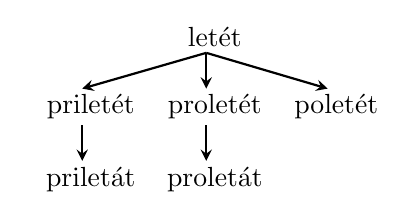
\begin{tikzpicture}
[
 baseline=(current bounding box.north), thick,
 >=stealth, outer sep=.5ex, inner sep=0ex
]
\node[matrix, minimum width=0ex, row sep=4ex, column sep=1.0ex, ampersand replacement=\&] at (0,0)
{
\& \node (v){~~let\'{e}t$^{{\IPF}}$}; \& \\
\node (priv) {~~prilet\'{e}t$^{{\PF}}$}; \&
\node (prov) {~~prolet\'{e}t$^{{\PF}}$}; \&
 \node (pov) {~~polet\'{e}t$^{{\PF}}$}; \\
\node (privi) {~~prilet\'{a}t$^{\DR{{\IPF}}}$}; \& 
\node (provi) {~~prolet\'{a}t$^{\DR{{\IPF}}}$}; \& \\
};
\draw[->] (v.south) -- (priv.north); 
\draw[->] (v.south) -- (prov.north); 
\draw[->] (v.south) -- (pov.north); 
\draw[->] (priv) -- (privi); 
\draw[->] (prov) -- (provi); 

%\node[text width=22ex] (provit)  at (0, -3) {`to fly some \textbf{distance}  or past something'};
%\draw[dashdotted, ->] (provi) -- (provit); 
\end{tikzpicture}
\hfill
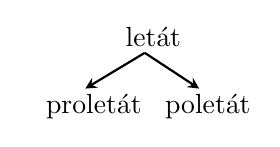
\begin{tikzpicture}
[
 baseline=(current bounding box.north), thick,
 >=stealth, outer sep=.5ex, inner sep=0ex
]
\matrix[minimum width=0ex, row sep=4ex, column sep=-3.0ex, ampersand replacement=\&]
{
\& \node (v){~~let\'{a}t$^{{\IPF}}$}; \& \\
\node (prov) {~~prolet\'{a}t$^{\DR{{\PF}}}$}; \& \&
 \node (pov) {~~polet\'{a}t$^{\DR{{\PF}}}$}; \\
};
\draw[->] (v.south) -- (prov.north); 
\draw[->] (v.south) -- (pov.north); 
%\node[text width=15ex] (provt)  at (-1.1, -3.55) {`to spend some \textbf{time} flying'};
%\draw[dashdotted, ->] (prov) -- (provt); 
\end{tikzpicture}
\hfill
\caption{Reanalysis of the traditional view (cf.~\figref{fig.traditional})}
\label{fig.reanalysis}
\end{figure}

%\citet[328]{Isachenko:60} writes that \citet{Regnell:44} has shown 
%nesti:nositi - \textit{nositi} is formed from \textit{nesti} (which is older) by making the route vowel longer. The correlation is indoeuropean. 
%``Das \"{u}bliche Ansicht ist, dass imperfektive Formen wie \textit{prinositi} und \textit{napadati} Zusammensetzungen mit dem ``iterativen'' \textit{nositi} und \textit{padati} sind. Demgem\"{a}ss betrachtet man sie als Ausnahmen von der Regel, dass ``ein einfaches Verbum durch Zusammensetzung perfectiv wird''.''
%Another kind of argumentation is provided by \citet[146]{Romanova:06}. She argues that the point of view under which prefixed imperfective verbs are thought of as being the result of the prefixation of an indeterminate verb, is wrong. However, the argumentation seems to be theory-internal: it is based on the assumption that indeterminate motion verbs cannot be combined with the lexical prefixes because the necessary syntactic position is occupied. 

Being left without any explanation in the literature defending the traditional view, let us turn to the alternative view, schematically represented on \figref{fig.reanalysis}. \citet{Regnell:44} provides the following two arguments in favor of analysing prefixed imperfective verbs of motion as secondary imperfectives of the prefixed determinate verbs. First, indeterminate motion verbs, such as \textit{nosit'}$_{\INDET}$ `to carry', contain (at least originally) a component of iterativity, while the corresponding prefixed imperfective verbs, such as \textit{prinosit'} `to bring/be bringing', lack it (this has been noticed already by \citealt{Mazon:1928}). Second, some verbs clearly do not follow the pattern ``indeterminate verb+prefix''. For example, \textit{priplyvat'} `to come/be coming by swimming' is not formed by \textit{pri-} + \textit{*plyvat'}, as the latter one does not exist. Generally speaking, only a subclass of motion verbs demonstrates what seems to be an exceptional behavior while another subclass produces regular secondary imperfective forms. Another point is that in other Slavic languages verbs similar to Russian ``exceptional'' ones are clearly the secondary imperfective forms and all the verbs that are the result of direct prefixation of motion verbs are perfective.

Another kind of argumentation is provided by \citet[146]{Romanova:06}. She argues that prefixed imperfective verbs cannot occur as a result of prefixation of indeterminate motion verbs because those verbs cannot be combined with lexical prefixes. Consider the verbs \textit{probeg\'{a}t'}$^{{\IPF}}$ `to be running past something' and \textit{prob\'{e}g{a}t'}$^{{\PF}}$ `to run for some time'. According to the theory advocated by \citet{Romanova:06}, the first verb contains a lexical prefix whereas the second verb contains a superlexical prefix. Romanova's analysis of motion verbs includes the assumption that the position for lexical prefixes is already occupied in the structure of a non-prefixed indeterminate motion verb. From this it follows that the verb \textit{probeg\'{a}t'}$^{{\IPF}}$ `to be running past something', that contains a lexical prefix, cannot be derived from the indeterminate motion verb \textit{begat'} `to run'. This argument is based on the assumption of syntactic differences between superlexical and lexical prefixes as well as specific differences in the internal syntactic structure of motion verbs. As this assumption is examined in Chapter~\ref{Chapter4} and I propose to abandon it in its current form, I will not go into further details of such an approach here.

\begin{figure}
\begin{center}
\hfill
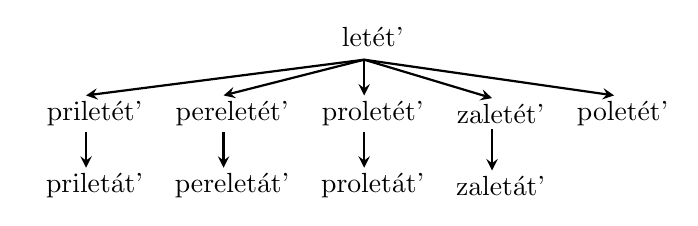
\begin{tikzpicture}
[
 baseline=(current bounding box.north), thick,
 >=stealth, outer sep=.5ex, inner sep=0ex
]
\node[matrix, minimum width=0ex, row sep=4ex, column sep=1.0ex, ampersand replacement=\&] at (0,0)
{
\& \& \node (v){~~let\'{e}t'$^{{\IPF}}_{\DET}$}; \& \&\\
\node (priv) {~~prilet\'{e}t'$^{{\PF}}$}; \&
\node (perev) {~~perelet\'{e}t'$^{{\PF}}$}; \&
\node (prov) {~~prolet\'{e}t'$^{{\PF}}$}; \&
\node (zav) {~~zalet\'{e}t'$^{{\PF}}$}; \&
 \node (pov) {~~polet\'{e}t'$^{{\PF}}$}; \\

\node (privi) {~~prilet\'{a}t'$^{{\IPF}}$}; \&
 \node (perevi) {~~perelet\'{a}t'$^{{\IPF}}$}; \&
\node(provi) {~~prolet\'{a}t'$^{{\IPF}}$}; \&
\node(zavi) {~~zalet\'{a}t'$^{{\IPF}}$}; \&\\
};
\draw[->] (v.south) -- (priv.north);
\draw[->] (v.south) -- (prov.north);
\draw[->] (v.south) -- (perev.north);
\draw[->] (v.south) -- (zav.north);
\draw[->] (v.south) -- (pov.north);
\draw[->] (priv) -- (privi);
\draw[->] (prov) -- (provi);
\draw[->] (perev) -- (perevi);
\draw[->] (zav) -- (zavi);

%\node[text width=22ex] (provit)  at (0, -3) {`to fly some \textbf{distance}  or past something'};
%\draw[dashdotted, ->] (provi) -- (provit);
\end{tikzpicture}
\hfill
\vspace{1cm}
\hfill
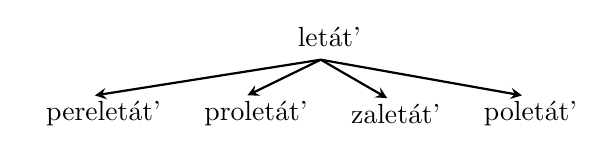
\begin{tikzpicture}
[
 baseline=(current bounding box.north), thick,
 >=stealth, outer sep=.5ex, inner sep=0ex
]
\matrix[minimum width=0ex, row sep=4ex, column sep=1.0ex, ampersand replacement=\&]
{
\&\&\& \node[inner xsep=-8ex] (v){~~let\'{a}t'$^{{\IPF}}_{\INDET}$}; \&\&\& \\
\node (perev) {~~perelet\'{a}t'$^{{\PF}}$}; \&\&
\node (prov) {~~prolet\'{a}t'$^{{\PF}}$}; \&\&
 \node (zav) {~~zalet\'{a}t'$^{{\PF}}$};\&\&
 \node (pov) {~~polet\'{a}t'$^{{\PF}}$}; \\
};
\draw[->] (v.south) -- (prov.north);
\draw[->] (v.south) -- (pov.north);
\draw[->] (v.south) -- (perev.north);
\draw[->] (v.south) -- (zav.north);

%\node[text width=15ex] (provt)  at (-1.1, -3.55) {`to spend some \textbf{time} flying'};
%\draw[dashdotted, ->] (prov) -- (provt);

\end{tikzpicture}
\hfill
\caption{Derivational trees for motions verbs}
\label{fig.reanalysis-all}
\end{center}
\end{figure}

From the discussion in the literature and the facts examined above I conclude that there are no solid reasons to consider prefixation of indeterminate motion verbs to be exceptional and non-perfectivizing. So let us stick to the derivations as they are presented on \figref{fig.reanalysis-all}, where all verbs that are obtained by prefixation from both determinate and indeterminate motion verbs are perfective and some can be consequently imperfectivized.

It is worth mentioning that the imperfectivization step that is included in the analysis represented on \figref{fig.reanalysis-all} is attested in Russian, though not very common. The following pairs represent such way of deriving imperfective verbs from the perfective source verbs: \textit{brosit'$^{{\PF}}$ -- brosat'$^{{\IPF}}$} `to throw', \textit{li\v{s}it'$^{{\PF}}$ -- li\v{s}at'$^{{\IPF}}$} `to deprive', \textit{re\v{s}it'$^{{\PF}}$ -- re\v{s}at'$^{{\IPF}}$} `to solve', \textit{kon\v{c}it'$^{{\PF}}$ -- kon\v{c}at'$^{{\IPF}}$}, \textit{prostit'$^{{\PF}}$ -- pro\v{s}\v{c}at'$^{{\IPF}}$} `to forgive', \textit{pustit'$^{{\PF}}$ -- puskat'$^{{\IPF}}$} `to let', \textit{obidet'$^{{\PF}}$ -- obi\v{z}at'$^{{\IPF}}$} `to offend', \textit{voskresit'$^{{\PF}}$ -- voskre\v{s}at'$^{{\IPF}}$} `to resurrect'.

There are still several verbs for which the formation of an imperfective from the prefixed perfective does not follow a regular pattern, e.g. \textit{prinesti}$^{{\PF}}$ `to bring' -- \textit{prinosit'}$^{{\IPF}}$ `to bring/be bringing' or \textit{prijti}$^{{\PF}}$ `to come' -- \textit{prixodit'}$^{{\IPF}}$ `to come/be coming'. The common suggestion is to explain the imperfectivization process in such cases by analogy, as it is done, e.g., by \citet{Regnell:44} and \citet[589]{Shvedova:82}. This problem lies in the area of historical linguistics as it requires the understanding of relative timing of different processes (emergence of certain verbs vs. formation of the aspect category in the contemporary sense) as well as the information about phonological rules applied throughout the centuries when the verbs in question were present in the language. This is why I will stick to the schema provided on \figref{fig.reanalysis-all} and leave the problem of irregular secondary imperfective formation aside.
%\fi

%\iffalse
\section{Prefixation and telicity}\label{section:new:telicity}
Whenever prefixes and perfectivity are mentioned, the issue of telicity arises. Although the thorough discussion of the relation between verbal aspect and telicity is outside the scope of this thesis, at least a few observations are in order. %For this reason I will only outline the problems that arise in connection with applying the notion of telicity to Russian, possible ways to go, and reasons why a conclusive discussion of this topic is not mandatory for achieving the goals of the current study and can be postponed.

Let us take a look at how telicity is characterized in the literature. For instance, \citet[3]{Rothstein:08a} writes that``[t]here is an intuitive agreement that telic predicates are completed or inherently bounded, but what exactly that means is very much under debate.'' This also means that there is no single definition of telicity on which everybody agrees. The second main issue has to do with a disagreement about the level of grammatical description at which the notion of telicity ought to be applied. Both these issues make it hard to apply any characterization of telicity across different languages. 
%  with Before the notion of telicity can be applied to Russian (or any other language) data, we need to have a definition at hand. However, as \citet[3]{Rothstein:08a} writes, ``There is an intuitive agreement that telic predicates are completed or inherently bounded, but what exactly that means is very much under debate.'' Another question that has to be answered is the level on which the notion of telicity is applied. The uncertainty about the exact definition and the domain of application makes it particularly hard to transfer the notion to other languages. 

Several paths can be adopted in this situation. First, a number of linguists take telicity in Slavic languages to be tightly connected with perfectivity and prefixation. For example, \citet{Borer:03} and \citet{vanHout:08}, among others, assume that Slavic prefixes encode telicity on the verb, from which it follows that all prefixed verbs are telic. This assumption was challenged by \citet{Filip:03} who pointed out that although it is plausible to regard all perfective verbs as semantically telic, prefixes cannot be viewed as perfectivity or telicity markers.  

Another approach, offered by \citet{PaduchevaPentus:08}, follows the opposite path: separate telicity and aspect. The authors talk about telicity of aspectless verbal predicates. I find this approach interesting but unnatural, as aspect in Russian is not an inflectional category. 

The notion of telicity has been originally developed on the basis of English data. The main tests used to identify telic predicates are (i) compatibility with temporal adverbials (\textit{in x time/for x time}) and (ii) interpretation in the progressive aspect. The second test cannot be obviously applied to Russian data, because Russian does not have a grammaticalized progressive aspect. Moreover, the existence of true aspectual pairs (pairs of verb forms that only differ in aspect, but not in their lexical content) in Russian is controversial.
% unless one accepts the ``aspectual pairs'' model of Russian verbal system, there is no unique correspondences between the imperfective and perfective verbs. 

What is left then is the first test, that indeed is often transferred to Russian as a semantic test for telicity: if an accusative time measure phrase (e.g., \textit{X \v{c}asov/minut} `for X hours/minutes') can be added to the verbal phrase, the verbal predicate is considered atelic; if a prepositional measure phrase (e.g., \textit{za X \v{c}asov/minut} `in X hours/minutes') can be added, the predicate is considered telic.

Example \ref{ex:navarila} illustrates the application of the test in the basic case: the verb is formally perfective, semantically telic, and compatible with \textit{za-}headed temporal adverbials. 

\exg.\label{ex:navarila}Ona svarila$^{\PF}$ sup za 3 \v{c}asa.\\
she s.boil.\glb{pst.sg.f} soup.\glb{acc} behind 3 hours\\
\vspace{0.5em}
`She cooked the soup in 3 hours.'

%\TODO:change everything to pochitat knigu
This test, however, does not work with all perfective telic verbs. It is neither obligatory for the telic verbal description to be compatible with the \textit{za}-headed temporal adverbial nor does such compatibility indicate that the predicate denotes a set of single completed events. Consider the prefix \textit{po-}. The verb \textit{po\v{c}itat'$^{\PF}$}`to read for some time' is perfective and it denotes a set of bounded reading events, but it is only compatible with accusative temporal adverbials, as illustrated by \ref{ex:pobrosal}.

\ex.\label{ex:pobrosal}\ag.\label{ex:pobrosal:delim}On po\v{c}ital knigu pjat' minut.\\
he po.read.\glb{pst.sg.m} book.\glb{sg.acc} five.\glb{acc} minute.\glb{pl.gen}\\
\vspace{0.5em}
`He read the book for 5 minutes.'
\bg.*On po\v{c}ital knigu za pjat' minut.\\
he po.read.\glb{pst.sg.m} book.\glb{sg.acc} behind five.\glb{acc} minute.\glb{pl.gen}\\

%On the other hand, an imperfective verb \textit{begat'} `to run' denotes sets of unbounded running events, but it is compatible with \textit{za-}headed time adverbial (under coerced interpretation as an unbounded series of bounded running events

%In case the direct object is plural, both delimitative and distributive interpretations of the verb are available. In case of the delimitative interpretation, similarly to \ref{ex:pobrosal}, only an accusative measure phrase can be used \ref{ex:pobrosal:pl:delim}. In case of the distributive interpretation, as in \ref{ex:pobrosal:pl:distr}, only the prepositional (\textit{za-}headed) measure phrase can be attached in order to indicate the time it took to throw all of the balls one by one. 
%
%\ex.\ag.\label{ex:pobrosal:pl:delim}On po\v{c}ital knigi pjat' minut.\\
%he \glb{po}.read.\glb{pst.sg.m} book.\glb{pl.acc} five.\glb{acc} minute.\glb{pl.gen}\\
%\vspace{0.5em}
%`He was throwing the ball for 5 minutes.'
%\bg.\label{ex:pobrosal:pl:distr}On po\v{c}ital knigi za tri \v{c}asa.\\
%he \glb{po}.read.\glb{pst.sg.m} book\glb{.pl} behind three.\glb{gen} hour.\glb{sg.gen}\\
%\vspace{0.5em}
%`He threw all the balls in 3 hours.'
%
%The distributive interpretation of the prefix \textit{po-} is also enforced if the direct object contains an overt quantifier, e.g. \textit{vse} `all.' In this case the delimitative interpretation is not available together with the possibility to add an accusative time measure phrase, as illustrated by \ref{ex:pobrosat:vse}.
%
%\ex.\label{ex:pobrosat:vse}\ag.*On pobrosal vse mja\v{c}i pjat' minut.\\
%he \glb{po}.threw.\glb{pst.sg.m} all.\glb{pl.acc} ball.\glb{pl.acc} five.\glb{acc} minute.\glb{pl.gen}\\
%\bg.On pobrosal vse mja\v{c}i za tri chasa.\\
%he \glb{po}.threw.\glb{pst.sg.m} all.\glb{pl.acc} ball\glb{.pl} behind three.\glb{gen} hour.\glb{sg.gen}\\
%\vspace{0.5em}
%`He threw all the balls in 3 hours.'

So if the compatibility with different temporal adverbials is regarded as a test for telicity for Russian, we would have to assume that some perfective verbs and even verb phrases (on the assumption that telicity is determined on the VP level, e.g. \citealt{Borer:05}) could be atelic. This is not a problem per se, but does not agree with the semantic definition: if, according to the definition of \citet[3]{Rothstein:08a} any predicate that denotes a set of either completed or bounded events is telic, then the verb \textit{po\v{c}itat'} `read for some time' and the verbal phrase \textit{po\v{c}itat' knigu} `read the book for some time' in \ref{ex:pobrosal:delim} are telic. From this it follows that compatibility with temporal adverbials in Russian cannot serve as a test for telicity in the sense of \citet{Rothstein:08a}

%This is clear if one compares \ref{ex:pobrosal0} with \ref{ex:brosal}, as these two examples differ exactly by the boundedness of the event of throwing the balls.

%\ex.\ag.\label{ex:pobrosal0}On pobrosal mja\v{c}.\\
%he \glb{po}.threw.\glb{pst.sg.m} ball.\glb{sg.acc}\\
%`He threw the ball for some time.'
%\bg.\label{ex:brosal}On brosal mja\v{c}.\\
%he threw.\glb{pst.sg.m} ball.\glb{sg.acc}\\
%`He was throwing the ball.'

%On Rothstein's definition pochitat' comes out telic + it is perfective, so the adverbial test is not a test.

Now the only path we are left with is the pure semantic definition of telicity: telic predicates are predicates that denote sets of bounded events. However, the application of this definition is not straightforward: there are cases for which it is hard to decide whether the set of events denoted by the verbal phrase contains only bounded events, especially when tenseless predicates are considered. For example, let us determine the telicity of the predicates in \ref{ex:telicity}.

\ex.\label{ex:telicity}\ag.\label{ex:telicity:soup}est' sup\\
eat.\glb{inf} soup.\glb{sg.nom}\\
eat soup
\bg.\label{ex:telicity:apple}est' jabloko\\
eat.\glb{inf} apple.\glb{sg.nom}\\
eat an/the apple

There will be probably no disagreement that the description \ref{ex:telicity:soup} (in absence of a context that would lead to a portion interpretation of the noun) is atelic. The second case is far less obvious: on one hand, the description involves a quantized object and the corresponding English description is telic, so it is tempting to consider the predicate \ref{ex:telicity:apple} to be telic. On the other hand, an event of partial consumption of an apple also falls under the denotation of \ref{ex:telicity:apple}. In addition, the combination of the verb \textit{est'} `to eat' with explicit measure phrases is not possible (without strong contextual support and inclusion of a time measure phrase), as illustrated by \ref{ex:telicity:2}. 

\ex.$^\#$est' dva litra supa \label{ex:telicity:2}\\
\textcolor{white}{$^\#$}eat.\glb{inf} two.\glb{m.acc} litre.\glb{sg.gen} soup.\glb{sg.gen}\\
\textcolor{white}{$^\#$}eat two litres of soup

This is unexpected if one considers that the telicity of the verb \textit{eat'} `to eat' is determined not by the verb, but by the properties of the direct object (incremental theme). My intuition is that \ref{ex:telicity:apple} is an atelic description, as the theme does not contribute the measure, only the type of the object that is being consumed. The difference between the acceptability of \ref{ex:telicity:apple} and \ref{ex:telicity:2} is, in my opinion, due to the flexibility of the interpretation of nouns: \textit{jabloko} `apple' can be viewed as a type description and it can be viewed as a measure (where area and volume of the apple can be used for establishing the boundary of the respective scale). At the same time \textit{sup} `soup' (unless it is used in the sense of `a portion of soup') is a pure type description and \textit{dva litra supa} `two litres of soup' is an overt measure description. These intuitions are summarized in Table~\ref{table:nouns}.

\begin{table}
\caption{Interpretation of noun phrases \label{table:nouns}}
\begin{tabular}{llcc}
\lsptoprule
nouno phrase & translation & type description & measure description\\\midrule
\textit{sup} & `soup' & + & \textminus \\
\textit{jabloko} & `apple' & + & + \\
\textit{dva litra supa} & `two litres of soup' & \textminus & +\\
\lspbottomrule
\end{tabular}
\end{table}

%The question addressed in numerous papers is whether (and how) one can predict the (a)telicity of a verbal predicate based on the information about its aspectual class (usually one of the four Vendler classes).
 
%A particular problem for the conception of telicity is posed by the perfective verbs with delimitative semantics, such as \textit{poletat'} `to fly for some time,' which refer to bounded and completed events of flying that can last arbitrary time (time boundary in not inherent and often not specified by the context, but nevertheless present). 
 
I will leave the further discussion of telicity in Russian for future work. However, I will provide some answers to the questions that are related to the notion of telicity. For English, saying that the predicate is telic is equivalent to saying that it is compatible with certain time measure adverbials and give rise (or not) to the imperfective paradox, as those properties are tied together. While leaving the notion of telicity outside of the upcoming discussion in Chapter~\ref{Chapter5}, I will provide an (somewhat implicit) answer to the question of compatibility of verbal predicates with various types of time frame adverbials: as soon as we have semantic representations of verbs, prefixes, noun phrases, and time measure phrases (see Chapter~\ref{Chapter7}) the compatibility and incompatibility will be predicted without using any extra features.

As for the conceptual part of the notion of telicity, it also will be present in my account, but deprived of the name that raises additional questions. The whole account that I offer is based on scales and measurement and, as was pointed out by \citet[60]{Rothstein:08}, ``Information about measurment cannot be ignored and the calculation of telicity is fully compositional, working from the verbal head upwards." So I will not label predicates except with the types that will be used in the semantic representations (and they will remind Vendler classes, as there are \textit{processes, states, events,} and \textit{transitions}) and I will use scales and measurement and composition to calculate the possible combinations of various elements. I will also use terms `bounded' and `unbounded' and define them with respect to the semantic representation of predicates. I will leave the mapping of these categories to the traditional notion of telicity and to the behaviour of the corresponding English verbs for future work.
 
\section{Summary}
In this chapter we have discussed the main issues related to perfectivity. First, I have presented the basic facts about aspectual opposition in Russian. Then we have explored existing approaches to the internal structure of complex verbs and found a group of verbs that are supposed to have different aspect under various accounts. Then we have proceeded with information about tests that help to identify aspect and I have shown that all the existing tests fail to distinguish imperfecive verbs from biaspectual ones. In order to fill this gap I have proposed a new test, that is based on the Narration relation. This test allows to identify in a positive way, whether a given verb can be used as a perfective verb, and thus serves to distinguish biaspectual verbs from perfective verbs.

In the next part of the chapter I have introduced the notions of derivational chains and a derivational graph. These instruments provide a possibility to explore the data in a more objective way and only exclude derivations that are not impossible in the language, regardless of the preferred theory of a given researcher. As the described graph does not exist in its full form, judgements on the following chapters are based on examples from corpora/web, where each derivation is checked against the proposed definition of a derivational chain.

The last part of the chapter addressed the issue of biaspectuality and imperfectivity in relation to prefixation. I have presented data concerning the attachment of the iterative prefix \textit{pere-} to secondary imperfective verbs and compared the behavior of mative and loaned biaspectual verbs and prefixes. In sum, the number of cases when prefixation does not lead to perfectivization turns out to be higher than traditionally assumed, but further research is needed to bring more clarity in this issue. On the other hand, as it have been shown in the very last part of the chapter, prefixed motion do not constitute an exception to the `prefixation leads to perfectivization' rule, contrary to numerous claims in the literature. In this respect, I have proposed evidence for an alternative analysis that does not require to postulate an exceptional group of motion verbs. With this, we are now ready to move on to a thorough discussion of lexical/superlexical division of prefixes.

%The prefix \textit{pere-} is similar to \textit{po-} in that it also has different interpretations and one of them is distributive. The verb \textit{peremyl} in \ref{ex:peremyl} can mean `rewash' as well as `wash all of'. However, both interpretations in case of \textit{pere-} are compatible only with prepositional time measure phrases. The use of an accusative time measure phrase is not licensed. Similar to what we have seen with \textit{po-}, uttering a quantifier phrase as a direct object forces a distributive interpretation of the verb (see example \ref{ex:peremyl:distr}).
%
%\exg. \label{ex:peremyl}On peremyl stakany za pjat' minut.\\
%he po.wash.\glb{pst.sg.m} glasses.\glb{pl.acc} behind five.\glb{acc} minutes\\
%\vspace{0.5em}
%`He washed all/rewashed the glasses in 5 minutes.'
%
%\exg. \label{ex:peremyl:distr}On peremyl vse stakany za pjat' minut.\\
%he po.wash.\glb{pst.sg.m} all.\glb{pl.acc} glasses.\glb{pl.acc} behind five.\glb{acc} minutes\\
%\vspace{0.5em}
%`He washed all/$^\#$rewashed all the glasses in 5 minutes.'
%
%Now let us explore the last prefix for this section, the prefix \textit{za-}. This prefix can have different interpretations and its contribution to the meaning of the derived verb is not always transparent, as, for example, in the pair \textit{pisat'} `to write' -- \textit{zapisat'} `to record.' There is, however, a regular meaning of the \textit{za-} prefix: inception. As an example, consider a pair of motion verbs \textit{begat'}$^{\IPF}$ `to run' -- \textit{zabegat'}$^{\IPF}$ `to start running.' The sentence in \ref{ex:zabegal:bare} illustrates how the prefixed verb may be uttered. It turns out that neither an accusative nor a prepositional time measure phrase can be added to the sentence \ref{ex:zabegal:bare}: \ref{ex:zabegal:za} is grammatical, but uninterpretable and \ref{ex:zabegal:acc} is ungrammatical.
%\ex.\label{ex:zabegal}\ag.\label{ex:zabegal:bare}On zabegal.\\
%he za.run.\glb{pst.sg.m} \\
%\vspace{0.5em}
%`He started to run.'
%\bg.$^\#$On zabegal za pjat' minut.\label{ex:zabegal:za}\\
%\textcolor{white}{$^\#$}he za.run.\glb{pst.sg.m} behind five.\glb{acc} minute.\glb{pl.gen}\\
%\bg.*On zabegal pjat' minut.\label{ex:zabegal:acc}\\
%he za.run.\glb{pst.sg.m} five.\glb{acc} minute.\glb{pl.gen}\\
%
%This observation does not apply to all the verbs prefixed with inchoative \textit{za-}: \ref{ex:zarabotat} is grammatical. It must be noted that in this case the time measure phrase refers to the duration of the preparatory phase. In our example \ref{ex:zarabotat} it would mean that someone worked for 4 hours to repair the computer and at the end of this period the computer (instantly) started to work. So in this case the measure phrase that denotes duration is in fact used to refer to a particular time point (immediately after the described period).
%
%\exg.\label{ex:zarabotat}Kompjuter zarabotal za \v{c}etyre \v{c}asa.\\
%computer za.work.\glb{pst.sg.m} behind four.\glb{acc} hour.\glb{sg.gen}\\
%\vspace{0.5em}
%`The computer started to work in four hours.'
%
%The data presented here adds a point to the previous discussion: neither the whole group of those prefixes that are called superlexical nor any subgroup of them according to the proposed analyses is homogeneous from the point of view of the commonly applied telicity test.
%
%%Another concern that arises when one considers the data presented here is that the Russian test for telicity does not perfectly correspond to the English original. 
%%\fi
%
%
%My view on English telicity: if one adopts scalar approach, telicity becomes a dependent notion. Activity verbs both do not require a scale and accept time scale as a valid input. On the other hand, measure phrases like \textit{for an hour} contribute the \textit{time} measure of change scale as a measure dimension of the event. Measure phrases like \textit{in an hour} do not describe any changes, as they do not play a role in determining when the event terminated. They only \textbf{describe} the time the event lasted. So they contribute duration, but not the measure of change scale. Accomplishments predicates require a scale and 
%
%activities are verbal phrases that do not require scales and accept time scale as a valid input; states do not require scales and do not accept time scales as input
%accomplishments 
%
%states can be only described in terms of time scales, static states 
%processes can be described in terms of scales other than time
%
%\begin{tabular}{l  l  l}
%& time scale allowed & time scale not allowed\\
%\hline \hline
%other scale realized & --  & protracted event\\
%\hline
%other scale allowed/lexicalized & process & culmination\\
%\hline
%other scale not allowed & dynamic state & non-scalar events
%
%\end{tabular}
%
%-- is explained by the \textit{one delimitation per event} constraint (a VP cannot contain two phrases with a function of measuring out, or delimiting the event (Filip 04, Goldberg 91, Levin and Rap Hovav 1995, Simpson 1983, Tenny 1994)
%non-scalar events: static states, happenings
%
%result state + for 2 minutes
%I opened the door for two minutes -- ambiguous (2 minues of opening or open state)
%--> Ja otkryval dver' 2 minuty/Ja otkryl dver' za 2 minuty
%
%``\textit{read} can take an incremental object, which can serve as a scale, but \textit{tickle} cannot" \citet[34]{Rappaport:08}
%
%``Information about measurment cannot be ignored and the calculation of telicity is fully compositional, working from the verbal head upwards." \citet[60]{Rothstein:08}
%
%Examples from \citet[61]{Rothstein:08}: \\
%(30a) Guests/help arrived in a few minutes\\
%(31a) Guests arrived for hours.\\
%The second reading is not available without the time measure phrase:\\
%\textit{Guests arrived} -> one event, all the guests arrived together\\
%So by default we have one event of transition with \textit{guests} as an actor. To get the second interpretation, we have to coerce it (multiple events using subsets of guests). So it feels to me that what is called atelic just can't be uttered without some kind of measure/delimitation (in simple past/present): ``Jon runs" can be interpreted as ``Jon is doing regular jogging" (coercion again). Different limitations are possible: 
%
%\ex.In this chapter I address the issue of telicity 
%
%cf.
%\ex.I address the issue of telicity (without context providing limitations)
%
%An account of this goes back to \citet{Taylor:77} and \citet{Dowty:79}, and \citet{Landman:08} discusses it in more detail. 
%
%static states as well as happenings are events that cannot be described using the notion of a scale: they have no inner development nor can they be related with a distinguished point of the development of some other event. Happenings do not develop because they are instantaneous (and independent of other events) while static states by definition do not represent any change nor are related to time. 
%
%Dynamic states, as states, do not have internal structure, but they are located in time and normally hold for a limited amount of time. 
%
%Processes are the only eventualities that can be described both in terms of time and in terms of some other scale. 
%
%A telic eventuality for me is an eventuality that \textbf{is} measured out in terms of some scale. An atelic eventuality is an eventuality that \textbf{can be} measured in terms of time. For this, it must have duration and not be already measured out. Note that such definition implies that the verbal predicate \textit{walk for 2 hours} is telic. 
%
%"Stative verbs involve no change" = stative verbs are such verbs that are not related to a progress on any scale (except for time).
%
%Expressivity of Russian verbal system is higher: scale selection and 

%\section{Conclusion}
%Although I may not always refer to the derivational graph and the test of perfectivity, introduced in this chapter, they will be used (at least implicitly) for all the data presented in the rest of the thesis. This means that whenever I describe some verb \textit{x} as being derived from some other verb \textit{y}, in the (mentally constructed) derivational graph as defined in Section~\ref{section:graph} there is only one incoming edge to the node that contains the verb \textit{y} and this edge goes out of the node that contains the verb \textit{x}. 
%
%The test for perfectivity, described in Section~\ref{section:new:perfectivity}, is also used every time I provide information about the aspect of the (complex) verb, even if there are no testing examples provided in the text. Explicit testing of all the verbs would lead to an unnecessary expansion of text, so except for the verbs that receive different aspect marking in the literature, I omit providing the test contexts.
%
%So this chapter, even if not referred to very often, provides a basis for all the work done in the subsequent parts of this thesis. 
 % Getting data right || A novel approach to the analysis of Russian complex verbs
% % Chapter 3

\chapter{Lexical and superlexical prefixes?} 
\label{Chapter4}
%\lhead{Chapter 3. \emph{Lexical and superlexical prefixes?}} % 
%The theoretical advances described in \ref{Chapter2} rule out a lot of impossible combinations of prefixes and makes the whole picture of Russian prefixation much more clear, but the following questions still remain unanswered:
%\begin{itemize}
%\item Why this or that prefix in a particular meaning falls in one or another group?
%\item Why the same prefixes with different meaning end up in different groups? Is there a theory-external explanation for this?
%\item Do the prefixes belonging to one group behave uniformly?
%\item Are that all the impossible combinations ruled out by the theory?
%\item Are all the combinations allowed predicted to be such by the theory?
%\end{itemize}
%As several researches have pointed out the problems with the superlexical/lexical distinction, I will start with an overview of the main points concerning this topic and continue with discussing the questions formulated above. 

%\section{Lexical and superlexical prefixes}\label{section:new:distinction}
This chapter discusses in detail the distinction between lexical and superlexical prefixes. This opposition constitutes the main driving force of the syntactic approaches to Russian prefixation (\citealt{Ramchand:04, Svenonius:04b, Romanova:06}, among others), as prefixes that belong to different groups are claimed to have distinct syntactic positions and properties. In what follows I provide details about the history and various refinements of this distinction and discuss problems that arise with it. I then show that neither the bipartite nor the more fine-grained distinctions are sufficient to account for the full range of data. Based on the observations about the vagueness of the distinction together with insufficient predictive power, I abandon the hypothesis that the formation of complex verbs depends primarily on the structural positions of the affixes and develop an alternative (semantic) approach in Chapter~\ref{Chapter5}.

 The methodology of gathering and assessing the data proposed in Chapter~\ref{Chapter2} will be (mostly implicitly) used throughout the discussion in this chapter, as it allows to identify examples that are problematic if one does not presuppose any linguistic theory prior to collecting the data.

The chapter is organized as follows: first, in Section~\ref{section:properties} I consider the main properties attributed to the prefixes of the superlexical group. In Section~\ref{section:classification} I look at the ambiguity of classification stemming from different works. Sections~\ref{section:new:compositionality}--\ref{section:new:position} discuss the problems that arise with each of the four properties attributed to the class of superlexical prefixes. Section \ref{section:subclasses} is dedicated to the more elaborated classifications proposed in \citet{Tatevosov:07,Tatevosov:09}. Section~\ref{section:new:conclusion} concludes the discussion.
\section{Main properties}\label{section:properties}
%\subsection{Lexical and superlexical prefixes}\label{extintpref}
The main idea of the classification discussed in this chapter has its origins in the long-standing tradition of distinguishing between two types of prefixes \citep{Isachenko:60, Forsyth:70, Townsend:75}: lexical prefixes (also called qualifying or internal prefixes) vs. prefixes that derive Aktionsart verbs (modifying in the terminology of \citeauthor{Isachenko:60}, later in the literature called superlexical or external).

The original idea of \citet[222--224]{Isachenko:60} is to divide verbal prefixes into two classes on the basis of their semantic contribution to the meaning of the derived verb. \citeauthor{Isachenko:60} writes that a qualifying prefix characterizes the verbal meaning from the outside, altering the lexical meaning of the derivational base. The derived verb acquires a meaning detached from the meaning of its input and becomes a new independent lexeme. A modifying prefix, on the other hand, does not change the lexical meaning of the derivational base, but rather emphasizes one of the inner characteristics of the process denoted by the non-prefixed verb.

As an example, \citet{Isachenko:60} provides prefixes \textit{raz-} and \textit{za-}: when the prefix \textit{raz-} is attached to the verb \textit{rvat'}\textsuperscript{\IPF} `to tear', the resulting verb \textit{razorvat'}\textsuperscript{\PF} acquires a new lexical meaning `to tear apart/to pieces'. When, on the other hand, the prefix \textit{za-} is attached to the verb \textit{govorit'}\textsuperscript{\IPF} `to talk', the meaning of the resulting verb \textit{zagovorit'}\textsuperscript{\PF} `to start talking' can be viewed as a shift of focus to to the initial phase of the event denoted by the derivational base.

\citet{Isachenko:60} also argues that verbs derived by the qualifying prefixes are grammatically distinct from the verbs derived by the modifying prefixes: the former and not the latter allow secondary imperfectivization. Note that in the original proposal by \citet{Isachenko:60} this is motivated by the semantics of the derived verb: whether it is distinct from that of the derivational base. This is the idea that I will (at least partially) return to in my analysis.

A couple of decades later the division of the prefixes into lexical\slash internal and superlexical\slash external\footnote{Note that the prefixes that, according to \citet{Isachenko:60}, modify the semantics of the verb \textit{externally}, are later called \textit{internal}, while prefixes that modify the \textit{internal} aspects of the process denoted by the derivational base are later called \textit{external}.} became the key component in contemporary (mostly syn\-tac\-tically-based) approaches to Russian prefixation \citep{Schoorlemmer:95, Babko-Malaya:99, Borik:02, Gehrke:04, Ramchand:04, Romanova:04, Romanova:06, Svenonius:04a, Svenonius:04b, DiSciullo:05}. Following \citet[229]{Svenonius:04b}, who builds on the discussion of Russian by \citet{Schoorlemmer:95}, these two\linebreak groups are distinguished according to the following diagnostics:

\begin{enumerate}
\item superlexical prefixes do not allow the formation of secondary imperfectives (invalid in Bulgarian), 
\item superlexical prefixes can occasionally stack outside lexical prefixes, never inside, 
\item superlexical prefixes select for imperfective stems, 
\item superlexical prefixes attach to the non-directed form of a motion verb,
\item superlexical prefixes have systematic, temporal or quantizing meanings, rather than spatial or resultative ones.
\end{enumerate}

\citet{Babko-Malaya:99} was the first to propose that the internal structure of complex verbs is represented by means of syntactic trees and lexical and superlexical prefixes occupy different syntactic positions in it. More precisely, lexical prefixes are adjoined to a lexical head, while superlexical prefixes are adjoined instead to a functional category. \citeauthor{Babko-Malaya:99} predicts that ``lexical prefixes modify the meaning of the verb, whereas superlexical prefixes are modifiers of verbal phrases or whole sentences'' \citep[76]{Babko-Malaya:99}. The (im)perfective aspect of a given complex verb is then determined by the properties of the highest affix in a structure. In what follows, let us have a look at a couple of proposals that follow this research program. 

\citet{Romanova:04} proposes the structure for Russian verbs that is represented on \figref{fig:romanova}. \citet[272]{Romanova:04} assumes ``the presence of AspP in between VP and vP'', that ``is a possible place for merge of the secondary imperfective suffix or purely perfectivizing prefixes''. She also postulates that lexical prefixes are located below AspP, while ``superlexical prefixes originate -- or at least end up -- above the AspP domain'' (p.~271). Throughout the paper, a lot of questions regarding the behavior of prefixes are posed and the author arrives at the conclusion that ``there is no uniform distribution of all superlexicals''.

\begin{figure}\small
% % \includegraphics[width=0.8\textwidth]{romanova.pdf}
\caption{\label{fig:romanova} Verbal structure according to \citet[272]{Romanova:04}}
\begin{forest}
[\textsc{dlmt}P
  [(for a while)]
  [\textsc{dlmt}'
    [\textit{po-}]
    [\textit{v}P
      [\textsc{originator}]
      [\textit{v}'
        [\textit{v}]
        [AspP
          [\textsc{undergoer}]
          [Asp'
            [\textit{(-i)va}\slash \textit{PPP}]
            [VP
              [X]
              [V'
                [V]
                [RP
                  [\textsc{resultee}]
                  [R'
                    [R]
                    [(PP)]
                  ]
                ]
              ]
            ]
          ]
        ]
      ]
    ]
  ]
]
\end{forest}
\end{figure}

While \citet{Babko-Malaya:99} and \citet{Schoorlemmer:95} (among others) assume that superlexical prefixes form a homogeneous class, \citet{Svenonius:04b} argues that there is a tripartite division among superlexical prefixes based on their ability to form secondary imperfectives.

According to \citet{Svenonius:04b}, certain superlexical prefixes (\textit{za-} with inceptive meaning, \textit{ot-} with terminative meaning, and \textit{pere-} with distributive meaning\footnote{\textit{pere-} has a variety of meanings (e.g. \citealt{Shvedova:82} distinguishes between 10 different meanings) including spatial, temporal, comparative, iterative, crossing the boundary, distributive and \textit{pere-} of excess. See Section~\ref{subsection:semantics:pere} for more information.}) may be attached higher than the structural position of the imperfective suffix, which is \textit{Asp}, the head of \textit{AspP}. Such prefixes disallow the formation of secondary imperfectives (e.g., \textit{za-} in its inceptive use). That is, the imperfective suffix cannot be directly attached to an imperfective stem and the result is an invalid structure (see \figref{fig:svenonius}).

There are also mixed cases like cumulative \textit{na-}, excessive \textit{pere-}, and attenuative \textit{po-}. The normal point of attachment of such prefixes, according to \citet[231]{Svenonius:04b}, is outside the scope of the secondary imperfective, however under certain exceptional conditions they allow a lower point of attachment.

Svenonius' main generalizations can be stated as follows (see also the summary in \citealt{Svenonius:12}): 

\begin{enumerate}
\item lexical prefixes originate inside \textit{v}P;
\item superlexical prefixes originate outside \textit{v}P;
\item lexical and superlexical prefixes that (according to him) disallow secondary imperfectivization are separated by Asp in the syntactic structure; 
\item exceptional superlexical prefixes are merged (sometimes) outside \textit{v}P, but below the Asp.
\end{enumerate}

\begin{figure}
% % \includegraphics[width=0.8\textwidth]{svenonius.pdf}
\begin{forest}
[AspP
  [PP [\textit{za-}\\\textsc{incp},align=center,roof]]
  [$\overline{\mbox{Asp}}$
    [Asp [(*\textit{-yvaj})]]
    [\textit{v}P
      [\textit{v}]
      [VP
        [\textit{kur-}\\`smoke',align=center]
      ]
    ]
  ]
]
\end{forest}
\begin{forest}
[AspP
  [Asp [-\textit{yvaj}]]
  [\textit{v}P
    [PP [\textit{pere-}\\\textsc{re},align=center,roof]]
    [\textit{v}P
      [\textit{v}]
      [VP [\textit{pis-}\\`write',align=center]]
    ]
  ]
]
\end{forest}
\caption{\label{fig:svenonius}Verbal structure according to \citet[231]{Svenonius:04b}}
\end{figure}

From another study that follows the same tradition, \citealt{Ramchand:04}, the following `bottom-up' order of verbal affixes emerges:

\begin{enumerate}
\item lexical prefixes;
\item aspectual head that may contain either the imperfective suffix or a superlexical prefix;
\item a DP projection for superlexical distributional prefixes (she cites \textit{pere}- and \textit{po}-). 
\end{enumerate}
While the motivation for this hierarchical order is not entirely clear, it would seem to derive from the following assumptions made by \citet{Ramchand:04}: 
\begin{enumerate}
\item lexical prefixes appear low in the syntactic structure, due to which a ``presuppositional structure to the aspectual head'' is introduced ``to the effect that it creates a definite rather than an indefinite time moment in Asp'' (p. 349);
\item most superlexical prefixes are in Asp and ``impose a specific reference time on the relation between event and temporal anchoring'' (p. 351);
\item a position that superlexical prefixes that are distributional (\textit{pere}- and distributive \textit{po}-) occupy is higher in the hierarchy than the Asp head (p. 352); such prefixes can be attached directly to the root or to the secondary imperfective verb.
\end{enumerate}
The fundamental two-way distinction is of key importance for \citet{Romanova:04}, \citet{Svenonius:04b}, and \citet{Ramchand:04}. Putting it simply, the main idea is that lexical prefixes occupy lower positions in the syntactic tree than the superlexical ones. Though it is possible that there is more than one position for superlexical prefixes, all such positions should be higher than the one (unique) position for the lexical prefixes. 

Due to this syntactic difference, superlexical prefixes are claimed to have the following properties:
\begin{enumerate}
\item they provide a systematic semantic contribution and do not change the lexical meaning of the verb;
\item they are incompatible with secondary imperfectivization;
\item they do not change the argument structure of the verb;
\item they appear to the left of the lexical prefixes (if two or more prefixes are stacked). 
\end{enumerate}

Lexical prefixes, on the other hand, are expected to change the lexical meaning of the verb, allow for secondary imperfectivization, change the argument structure of the verb, and always appear closer to the stem when prefix stacking occurs. At the same time two lexical prefixes can never stack, as there is a single position where they are allowed. While specific analyses vary a lot, this general idea remains the same. 

The distinction between the lexical and superlexical prefixes has received some amount of criticism in the recent literature. For example, \citet{Braginsky:08}, analyzing different usages of the prefix \textit{za-}, arrives at the conclusion that ``the contrasts
between inchoative and non-inchoative prefixes ZA- cannot be accounted for by
simply relating them to different structural positions on the syntactic tree'' (p. 224). Let me now analyse in detail properties that are attributed to superlexical prefixes and problems that arise when one tries to use the lexical/superlexical distinction for analysing complex verbs in Russian.

%The assumptions listed above lead to the certain predictions about the grammatical aspect of a given complex verb. First, if a verb contains a prefix and no imperfective suffix, it is perfective (see ex.~\ref{pred1}). Second, if a verb contains a lexical prefix and the imperfective suffix, it is imperfective (see ex.~\ref{pred2}). Finally, if a verb contains a superlexical prefix and the imperfective suffix, it is perfective (see ex.~\ref{pred3}).

\section{Classification ambiguity}\label{section:classification}
The general problem of the lexical/superlexical distinction has been pointed out by \citet[32]{Kagan:book}: many prefixes are not easily classified as either lexical or superlexical as they do not have the whole cluster of properties of one of the groups, but rather a mixture of those. This results in a range of classifications offered by different researchers. Table \ref{table:prefixes} summarizes various proposals in this respect.


\begin{table}
\caption{Superlexical prefix inventory according to different studies\label{table:prefixes}}
\begin{tabular}{lccccccc}
\lsptoprule
prefix &  \rotatebox{90}{\citet{Babko-Malaya:99}} & \rotatebox{90}{\citet{Svenonius:04a}} & \rotatebox{90}{\citet{Svenonius:04b}\footnote{\citet{Svenonius:04b} provides a classification of Russian prefixes from the point of view of the formation of the secondary imperfective, but does not say anywhere that the list is extensive.}} & \rotatebox{90}{\citet{Ramchand:04}} & \rotatebox{90}{\citet{Romanova:06}} & \rotatebox{90}{\citet{Tatevosov:09}} & \rotatebox{90}{\citet{Svenonius:12}\footnote{\citet{Svenonius:12} marks the list as taken from \cite{Svenonius:04a}, but the lists vary significantly.}}\\
\midrule
inchoative \textit{za-} & + & + & + & + & + & + & +\\
cumulative \textit{na-} & \textminus & + & + & + & + & + & +\\
saturative \textit{na-} & \textminus & + & \textminus & \textminus & \textminus & \textminus & +\\
repetitive \textit{pere-} & \textminus & + & + & \textminus & \textminus & + & +\\
excessive \textit{pere-} & \textminus & + & + & \textminus & \textminus & \textminus & +\\
distributive \textit{pere-} & \textminus & \textminus & + & \textminus & + & + & +\\
distributive \textit{po-} & \textminus & + & \textminus & \textminus & + & + & +\\
delimitative \textit{po-} & + & + & \textminus & + & + & + & +\\
attenuative \textit{po-} & \textminus & + & + &  \textminus & \textminus & \textminus & +\\
attenuative \textit{pri-} & \textminus & \textminus & \textminus & \textminus & + & \textminus & \textminus\\
attenuative \textit{pod-} & \textminus & \textminus & \textminus & \textminus & + & + & \textminus\\
terminative \textit{ot-} & \textminus & + & + & \textminus & + & \textminus & +\\
perdurative \textit{pro-} & + & + &  \textminus & \textminus & \textminus & \textminus & +\\
completive \textit{iz-} & \textminus & + & + & \textminus & \textminus & \textminus & +\\
completive \textit{do-} & \textminus & + &  \textminus & + & \textminus & + & +\\
\lspbottomrule
\end{tabular}
\end{table}

The rows of Table~\ref{table:prefixes} show ten prefixes (\textit{za-, na-, pere-, po-, pri-, pod-, ot-, pro-, iz-, do-}) together with their interpretations (up to three in case of the prefixes \textit{pere-} and \textit{po-}). The columns of the table represent seven different proposals: \citealt{Babko-Malaya:99}, \citealt{Svenonius:04a}, \citealt{Svenonius:04b}, \citealt{Ramchand:04}, \citealt{Romanova:06}, \citealt{Tatevosov:09}, and \citealt{Svenonius:12}. A plus in the intersection indicates that the prefix of the row (with the fixed interpretation) is listed as superlexical in the work that names the column. As lexical prefixes are usually not explicitly listed, a minus in the intersection only indicates that the prefix with specific meaning is not listed as superlexical.

As is evident from the table, there is only one prefix that is overtly classified as superlexical in all the discussed studies: the inchoative prefix \textit{za-}. For two more prefixes, cumulative \textit{na-} and delimitative \textit{po-}, the consensus is almost met: all but one study describe them as being superlexical. Among the remaining prefixes, there is no single prefix listed as superlexical in 5 out of 7 discussed works. After this gap comes a group of prefixes that are accepted to be superlexical in most accounts represented in the table: repetitive \textit{pere-}, distributive \textit{pere-}, distributive \textit{po-}, terminative \textit{ot-}, and completive \textit{do-}. This makes a total of 3 prefixes being in the ``strong'' group and 5 more being in the ``weak'' group. Further 7 prefixes are considered superlexical only in a couple of studies. Note that there is no pair of works with identical lists of superlexical prefixes. 

Such variability in the decisions about which prefix (even under a particular interpretation) falls into one of the two groups (lexical or superlexical) clearly shows that this distinction is problematic: the properties that are claimed to be associated with the superlexical prefixes do not come together. I believe that they are not completely independent of each other, but the connection is weaker than is commonly assumed. Let us now discuss different properties attributed to the members of the superlexical class of prefixes and see if they are supported by the language data.



\section{Semantics of the derived verb}\label{section:new:compositionality}
The compositionality of meaning is one of the main characteristics of the superlexical prefixes, as follows from the summary provided in Section~\ref{section:properties}. It is important to note, however, that this property is not very valuable in case we classify prefixes together with certain fixed interpretations. For instance, if one takes into account only inchoative usages of \textit{za-}, then verbs formed with the inchoative prefix \textit{za-} will all have the meaning of inception of the activity described by the derivational base. All the other \textit{za-}prefixed verbs, even if their semantics is perceived as being close to that of inception, will remain outside of the focus set of verbs. This means that when the prefix usages are classified, the property of contributing a compositional meaning is reduced to the productivity of a particular meaning of a given prefix. This said, one has to note that many prefixes that are classified as lexical have systematic transparent contributions: e.g., spatial prefixes when combined with motion verbs. Consider, in particular, the spatial usage of the prefix \textit{pere-}, `to cross'. Whenever this prefix is attached to a directed motion verb, it contributes the meaning `to cross something in a manner denoted by the derivational base', that can also be reformulated as `to perform the motion denoted by the derivational base along the path that crosses the landmark'. However, this prefix (and other similar ones) is not considered as being superlexical.

One may reply at this point, that it is not only the systematic semantic contribution, but the absence of change in the lexical meaning, that distinguishes superlexical prefixes from lexical ones. Let us consider the verb \textit{proplyt'}\textsuperscript{\PF} `to swim a certain distance' and the verb \textit{proplavat'}\textsuperscript{\PF} `to swim for a certain time'. In the first case we are dealing with the spatial interpretation prefix \textit{pro-} that is considered to be lexical, while in the second case the same prefix is interpreted temporarily and is considered to be superlexical by \citet{Babko-Malaya:99}, \citet{Svenonius:04a}, and \citet{Svenonius:12}. Given the semantics of the derived verbs and the possibility of the unified analyses of the prefix \textit{pro-} in these cases \citep{Kagan:book, ZinovaOsswald:paper}, it would be very hard to argue that one of those prefixes affects the lexical meaning of the verb, while the other does not. 

\section{Secondary imperfectivization}\label{section:new:imperfectivization}
Another criterion that is used for establishing the lexical/superlexical status of a prefix with a fixed interpretation, is the (un)availability of the secondary imperfectivization. Basically, superlexically prefixed verbs should not allow secondary imperfectivization while lexically prefixed verbs should be easily imperfectivized. Unfortunately, things are not as clear and there are exceptions from this rule in both directions. 

To overcome this difficulty, \citet{Svenonius:04b} and \citet{Tatevosov:07, Tatevosov:09} propose to split superlexical prefixes in further groups and distinguish subclasses of superlexical prefixes that allow subsequent imperfectivization. Note that in this case the property of having potential for further imperfectivization, that is used to delimit the classes, is not derived from other properties of the prefixes.

Furthermore, as is noted by \citet[35]{Kagan:book}, it is not the case that the availability of the secondary imperfective verb can be predicted from the knowledge about the last prefix attached to the verb (and its meaning). Distinct stems, when combined with the same prefix (with a fixed interpretation) behave differently: e.g., the verb \textit{naest’sja} `to eat one's fill' is easily imperfectivized and the combination of the verb \textit{nasmotret'sja} `to spend enough time looking at something' with an imperfective suffix is weird (example taken from \citealt[35]{Kagan:book}).

Let us examine the inchoative prefix \textit{za-} that both \citet[230]{Svenonius:04b} and \citet[116]{Tatevosov:09} take to disallow subsequent imperfectivization. Consider the verb \textit{kurit'}\textsuperscript{\IPF} `to smoke'. It can be prefixed with the inchoative prefix {\textit{za-}.} The output of prefixation is the verb \textit{zakurit'}\textsuperscript{\PF} `to start smoking'. This is a superlexically prefixed verb, according to the common classification, with the most prototypical superlexical prefix: the only one which is included in the superlexical group in all of the studies I examined. However, this verb can be further imperfectivized. The result of this operation is an imperfective verb \textit{zakurivat'}\textsuperscript{\IPF} `to start/be starting smoking'. As the verb \textit{zakurit'} `to start smoking' denotes a punctual event, the natural interpretation of the verb \textit{zakurivat'} `to start/be starting smoking'  is that of a habitual event. Consider example \ref{ex:zakurivat1}. In this sentence the speaker describes his regular activity: after some other event, he always started to smoke and smoked 10 cigarettes in a row. 

\exg.\label{ex:zakurivat1}Ja zakurival i kuril desjat' \v{s}tuk, ne vstavaja s mesta, odnu za drugoj.\\
I za.smoke.imp.\glb{pst}.\glb{sg}.\glb{m} and smoke.\glb{pst.sg.m} ten piece.\glb{pl.acc}, not get.up.imp.\glb{cvb}.\glb{pres} from place, one behind other\\
\trans `I started to smoke and smoked 10 cigarettes one after another without getting up.'\hbox{}\hfill\hbox{Vasilij Aksenov, \textit{Zvezdnyj bilet}}

At the first sight it seems impossible to interpret the resulting imperfective verb progressively. If this would be true, than a possible solution to the problem could be the one by \citet{Ramchand:04}. \citet{Ramchand:04} suggests that secondary imperfective forms with a habitual reading may be derived by a different imperfectivizing operator than secondary imperfective forms with a progressive reading. The operator with a habitual reading should be than situated higher than the superlexical prefix. This proposal does not solve the problem, as it turns out that progressive interpretation of the secondary imperfective verb containing the inchoative \textit{za-} is possible. Out of the blue a native speaker of Russian (without linguistic training) would probably deny the existence of such reading, but all the speakers I have consulted with accept the sentence \ref{ex:zakurivat2}. The trick here is to find some other event (in this case it is a glance) that takes even less time, and hence is ``more punctual''. Then the event of lightning a cigarette can be viewed as a progressive one. We will discuss this issue in more detail in the next chapter.

\exg.\label{ex:zakurivat2}Arkadij Sergeevi\v{c} kak raz zakurival, po\`{e}tomu ne zametil, kak na poslednej fraze Olafson po\v{c}emu-to vorovato strel'nul glazami.\\
Arkadij Sergeevich as time za.smoke.imp\glb{.pst.sg.m}, {that is why} not notice.\glb{pst.sg.m}, as on last phrase Olafson {because of something} thievishly shoot.sem.\glb{pst.sg.m} eye.\glb{pl.inst}\\
\trans `Arkadij Sergeevich was just lightning the cigarette, so he didn't notice Olafson's thievish glance during the last phrase.'\\\hbox{}\hfill\hbox{
Andrej Konstantinov, \textit{Vydum\v{s}\v{c}ik}}

Interestingly, while \citet{Tatevosov:09}, along with \citet{Svenonius:04b}, \citet{Ramchand:04}, and others, postulates the impossibility of subsequent imperfectivization of the verbs prefixed with inchoative \textit{za-} (p.~116), the theory described in the paper does not prohibit it, as \textit{za-} belongs to the group of prefixes that only attach to imperfective verbs (more details will follow in Section~\ref{section:Tat09}). This restriction is met in the example above: the verb \textit{kurit'}\textsuperscript{\IPF} `to smoke' is imperfective. It turns out that for \citet{Tatevosov:09} the only group of prefixes that disallows subsequent imperfectivization is the group of left periphery prefixes that is populated by only one prefix: distributive \textit{po-}. This amounts to the fact that one of the main properties of superlexical prefixes is attributed to just one prefix that is, moreover, not listed as superlexical by some authors.

On the basis of the facts described above I conclude that the availability of the secondary imperfective form can be neither used for classification purposes nor be reliably predicted from the lexical/superlexical status of a given prefix.

\section{Argument structure}\label{section:new:argstructure}
One more property that is said to be associated with superlexical prefixes is that they do not change the argument structure of the verb (while lexical prefixes do). As this criterion is also not unproblematic, \citet[116]{Tatevosov:09}, for example, adopts a milder version of the statement, namely, that superlexical prefixes either do not change the argument structure of the verb or restrict the possibilities of argument structure variation in a predictable way. However, there are exceptions to this property even in the latter formulation. 

The crucial example here is the cumulative prefix \textit{na-}, as it is considered to be superlexical in most of the studies. However, its attachment changes the argument structure of the verb: verbs that are optionally transitive when unprefixed become obligatorily transitive after the attachment of the cumulative \textit{na-}, as illustrated by \ref{ex:pref:na1}--\ref{ex:pref:na2}.

\ex.\label{ex:pref:na1}\ag.\label{ex:pref:na1a}Ma\v{s}a s\v{c}itaet\textsuperscript{\IPF} do desjati.\\
Ma\v{s}a count.\glb{pres.3.sg} until ten\\
\trans `Masha can count up to ten.'
\bg.*Ma\v{s}a nas\v{c}itaet\textsuperscript{\PF} do desjati.\label{ex:pref:na1b}\\
Ma\v{s}a na.count.\glb{pres.3.sg} until ten\\

\ex.\label{ex:pref:na2}\ag.*Ma\v{s}a s\v{c}itaet\textsuperscript{\IPF} desjat' konfet.\label{ex:pref:na2a}\\
Ma\v{s}a count.\glb{pres.3.sg} ten.\glb{acc} candies.\glb{gen}\\
\bg.\label{ex:pref:na2b}Ma\v{s}a nas\v{c}itaet\textsuperscript{\PF} desjat' konfet.\\
Ma\v{s}a na.count.\glb{pres.3.sg} ten.\glb{acc} candies.\glb{gen}\\
\trans `Masha's count of candies will be ten.'

This could be still in accordance with the proposal of \citet{Tatevosov:09}, but it turns out that the prefixed verb also provides an additional restriction on the direct object: it must be a measure phrase. The unprefixed verb \textit{s\v{c}itat'}\textsuperscript{\IPF} `to count/be counting' takes as a direct object any plural accusative noun phrase (see example \ref{ex:pref:na2a}), whereas the prefixed verb \textit{nas\v{c}itat'}\textsuperscript{\PF} `to count a lot of' does not (see example \ref{ex:pref:na2b}). It requires a measure phrase (example \ref{ex:pref:na3b}), which is not a valid direct object in case of the unprefixed verb \ref{ex:pref:na3a}. 

\ex.\label{ex:pref:na3}\ag.\label{ex:pref:na3a}Ma\v{s}a s\v{c}itaet\textsuperscript{\IPF} konfety.\\
Ma\v{s}a count.\glb{pres.3.sg} candies.\glb{acc}\\
\trans `Masha counts candies.'
\bg.*Ma\v{s}a nas\v{c}itaet\textsuperscript{\PF} konfety.\label{ex:pref:na3b}\\
Ma\v{s}a na.count.\glb{pres.3.sg} candies.\glb{acc}\\

As a result, in all three pairs of examples above involving the verbs \textit{s\v{c}itat'/nas\v{c}itat'} `to count' only one variant (either unprefixed or prefixed) is possible. The unprefixed verb is required in case of an indirect object, as in \ref{ex:pref:na1}, and in case of a direct object that is not a measure phrase, as in \ref{ex:pref:na2}. Only the prefixed verb can be used when the direct object is a measure phrase, as in example \ref{ex:pref:na3}. In fact, there seems to be no construction in which both \textit{s\v{c}itat'} `to count' and \textit{nas\v{c}itat'} `to count a lot of' could be felicitously uttered.

If one considers a pair where the unprefixed verb is obligatorily transitive, as \textit{varit'}\textsuperscript{\IPF} `to cook/be cooking' and \textit{navarit'}\textsuperscript{\PF} `to cook a lot of', it turns out these two verbs require different cases of the object. If the object is an accusative noun phrase \ref{ex:pref:navarit:1}, it is only compatible with the unprefixed verb. If it is a genetive noun phrase, it is only compatible with the prefixed member of the considered pair, as illustrated by \ref{ex:pref:navarit:2}.

\ex.\label{ex:pref:navarit:1}\ag.\label{ex:varit:1}Ma\v{s}a varit\textsuperscript{\IPF} sup.\\
Ma\v{s}a cook.\glb{pres.3.sg} soup.\glb{acc}\\
\trans `Masha cooks soup.'
\bg.*Ma\v{s}a navarit\textsuperscript{\PF} sup.\label{ex:navarit1}\\
Ma\v{s}a na.cook.\glb{pres.3.sg} soup.\glb{acc}\\

\ex.\label{ex:pref:navarit:2}\ag.*Ma\v{s}a varit\textsuperscript{\IPF} supa.\label{ex:varit2}\\
Ma\v{s}a cook.\glb{pres.3.sg} soup.\glb{gen}\\
\bg.\label{ex:navarit2}Ma\v{s}a navarit\textsuperscript{\PF} supa.\\
Ma\v{s}a na.cook.\glb{pres.3.sg} soup.\glb{gen}\\
\trans `Masha will cook a lot of soup.'

Interestingly, in the case of the pair \textit{varit'}\textsuperscript{\IPF} `to cook/be cooking' and \textit{navarit'}\textsuperscript{\PF} `to cook a lot of', a measure phrase can be used as a direct object with both verbs, as illustrated by \ref{ex:pref:navarit:3}.

\ex.\label{ex:pref:navarit:3}\ag.\label{ex:varit3}Ma\v{s}a varit\textsuperscript{\IPF} 5 litrov supa ka\v{z}dyj den'.\\
Ma\v{s}a cook.\glb{pres.3.sg} 5 litre.\glb{pl.gen} soup.\glb{gen} every day\\
\trans `Masha cooks 5 litres of soup every day.'
\bg.\label{ex:navarit3}Ma\v{s}a navarit\textsuperscript{\PF} 5 litrov supa.\\
Ma\v{s}a na.cook.\glb{pres.3.sg} 5 litre.\glb{pl.gen} soup.\glb{gen}\\
\trans `Masha will cook 5 litres of soup.'

This suffices to show that prefixes that are considered to be superlexical can change the argument structure of the verb, thereby not only limiting the existing options for the derivational base verb, but also adding new ones.

Now we consider the other direction: if the attachment of a superlexical prefix can lead to changes in the argument structure of the derivational base verb, we can try to reformulate the property. Alternative formulation would be to postulate that if a lexical prefix is attached to a verb, argument structures of the source and the derived verb will be distinct. This, however, does not work either. As an example, consider the pair of verbs \textit{delat'/sdelat'} `to do'. Both verbs are obligatorily transitive. Illustrations of this fact are provided in \ref{ex:delat} and \ref{ex:sdelat}.

\ex.\label{ex:delat}\ag.Petja delaet\textsuperscript{\IPF} doma\v{s}nee zadanie.\\
Petja do.\glb{pres.3.sg} home.\glb{sg.acc} assignment.\glb{sg.acc}\\
\trans `Petja is doing homework.'
\bg.*Petja delaet\textsuperscript{\IPF}.\\
Petja do.\glb{pres.3.sg}\\

\ex.\label{ex:sdelat}\ag.Petja sdelaet\textsuperscript{\PF} doma\v{s}nee zadanie.\\
Petja s.do.\glb{pres.3.sg} home.\glb{sg.acc} assignment.\glb{sg.acc}\\
\trans `Petja will do homework.'
\bg.*Petja sdelaet\textsuperscript{\PF}.\\
Petja s.do.\glb{pres.3.sg}\\


As one may object that the prefix \textit{s-} in \textit{sdelat'} `to do' is what some researchers call an ``empty prefix'' (a prefix that changes the aspect, but does not lead to a clear change of the lexical meaning, \textit{\v{c}istovidovaja pristavka} in Russian tradition), let me provide another example where the prefix is clearly not an ``empty'' one, but, according to those who use the lexical/superlexical distinction, a lexical one.  Consider the following three verbs: \textit{nesti\textsuperscript{\IPF}} `to carry', \textit{prinesti\textsuperscript{\PF}} `to carry to some destination',  and \textit{otnesti\textsuperscript{\PF}} `to carry away from some location'. All three verbs have the same argument structure: they are obligatorily transitive (see examples \ref{ex:nesti}--\ref{ex:otnesti}).

\ex.\label{ex:nesti}\ag.Petja nes\"{e}t\textsuperscript{\IPF} korobku v podval.\\
Petja carry.\glb{pres.3.sg} box.\glb{sg.acc} in cellar.\glb{sg.prp}\\
\trans `Petja is carrying the box to the cellar.'
\bg.*Petja nes\"{e}t\textsuperscript{\IPF} v podval.\\
Petja carry.\glb{pres.3.sg} in cellar.\glb{sg.prp}\\

\ex.\label{ex:prinesti}\ag.Petja prines\"{e}t\textsuperscript{\PF} korobku v podval.\\
Petja pri.carry.\glb{pres.3.sg} box.\glb{sg.acc} in cellar.\glb{sg.prp}\\
\trans `Petja will carry the box to the cellar.'
\bg.*Petja prines\"{e}t\textsuperscript{\PF} v podval.\\
Petja pri.carry.\glb{pres.3.sg} in cellar.\glb{sg.prp}\\

\ex.\label{ex:otnesti}\ag.Petja otnes\"{e}t\textsuperscript{\PF} korobku v podval.\\
Petja ot.carry.\glb{pres.3.sg} box.\glb{sg.acc} in cellar.\glb{sg.prp}\\
\trans `Petja will carry the box to the cellar.'
\bg.*Petja otnes\"{e}t\textsuperscript{\PF} v podval.\\
Petja ot.carry.\glb{pres.3.sg} in cellar.\glb{sg.prp}\\

This clearly shows that knowing the lexical or superlexical status of a prefix is not sufficient to predict whether its attachment will change the argument structure of the derivational base verb.
\section{Position in the stem}\label{section:new:position}
The least problematic property of superlexical prefixes is that they always appear to the left of the lexical prefixes if two or more prefixes are stacked. When formulated this way, the property holds. However, a stronger version of this statement is used in the literature, either explicitly \citep{Svenonius:04b} or implicitly \citep{Tatevosov:09}: as there is only one syntactic position a lexical prefix can appear in, it is assumed that lexical prefixes can only appear directly to the left of the verbal root and cannot be stacked. For example, \citet[206]{Svenonius:04b} writes: ``lexical prefixes are unique in each VP, as their structural position is unique -- a single V cannot have more than one resultative complement.''


This, however, does not hold. Consider, for example, the verb \textit{razukrasit'} `to decorate' and the verb \textit{razuznat'} `to find out'. Each of these verbs contains two prefixes, \textit{raz-} and \textit{u-}, both of which are lexical: if one consults again the Table~\ref{table:prefixes}, one would not find either of the prefixes classified as superlexical in any of the discussed papers. The derivation chains for the verbs are constructed using the criteria formulated in Chapter~\ref{Chapter2} and provided in \ref{schema:razukrasit'} and \ref{schema:razuznat'}.

\ex.\ag.\label{schema:razukrasit'}krasit'\textsuperscript{\IPF} {$\rightarrow$} ukrasit'\textsuperscript{\PF} {$\rightarrow$} razukrasit'\textsuperscript{\PF}\\
{to paint} {} {to embellish} {} {to decorate}\\
\bg.\label{schema:razuznat'}znat'\textsuperscript{\IPF} {$\rightarrow$} uznat'\textsuperscript{\PF} {$\rightarrow$} razuznat'\textsuperscript{\PF}\\
{to know} {} {to learn} {} {to find out}\\
\bg.*lo\v{z}it'\textsuperscript{\IPF} {$\rightarrow$} polo\v{z}it'\textsuperscript{\PF} {$\rightarrow$} raspolo\v{z}it'\textsuperscript{\PF}\label{schema:raspolozit'}\\
{to put} {} {to put} {} {to position}\\

Similar case is presented in \ref{schema:raspolozit'}
with the difference that in contemporary literal Russian the unprefixed verb \textit{*lo\v{z}it'\textsuperscript{\IPF}} does not exist (it exists in the colloquial language and in the dialects). 

From observing these three examples one may, for the sake of saving the hypothesis of a single position for lexical prefixes, hypothesize that the prefix \textit{raz-/ras-} is a superlexical one. The problem with this hypothesis is that if one believes that the contributions of lexical and superlexical prefixes have particular characteristics, then the semantics of this prefix patterns with the semantics of lexical prefixes: a thorough study is performed by \citet{JandaNesset:10}, who list 11 subclasses for the meaning that is contributed by the prefix \textit{raz-}, only one of them of  type that is characteristic of the typical contribution of a superlexical prefix (Complex Act Perfective in their terminology).

%\iffalse

\section{Subclasses of superlexical prefixes}\label{section:subclasses}
So far we have observed that the binary distinction between lexical and superlexical prefixes is not sufficient to predict the existence and properties of verbs containing certain sets of affixes. As at least some of the problems mentioned above were noticed by the researchers working on Russian prefixation, several refinements of the original distinction were proposed in the literature. In further developments of Russian prefixation theories we see a shift of focus from the bipartite distinction to the split of the whole class of prefixes into more than two groups: \citet{Tatevosov:07} proposes a three-way classification of verbal prefixes and \citet{Tatevosov:09} splits the class of superlexical prefixes into three subclasses.

\subsection{Intermediate prefixes}
\cite{Tatevosov:07} introduces a class of intermediate prefixes that is supposed to accommodate prefixes that do not fit nicely into neither lexical nor superlexical category. This class is populated by the completive prefix \textit{do-} and the repetitive prefix \textit{pere-}. \citet{Tatevosov:07} proposes that these prefixes are structurally higher than lexical prefixes, but lower than superlexical prefixes and the secondary imperfective. 

This division is motivated by examples like \ref{ex:naperf} and \ref{ex:pereimp}. For the analysis that assumes the two-way classification of prefixes, the verbs \ref{ex:naperf} and \ref{ex:pereimp} have identical internal structure: a superlexical prefix, a lexical prefix, a stem, and the imperfective suffix. Nevertheless, these verbs are assigned different aspects: the verb \textit{nazapisyvat'} `to write down a lot' is perfective while the verb \textit{perezapisyvat'} `to be rewriting/to rewrite' is imperfective. For \citet{Tatevosov:07}, there is a structural difference between the two verbs, because \textit{pere}- is classified as an intermediate prefix and is positioned between lexical prefixes and the imperfective suffix. As a result, the verb in \ref{ex:pereimp} gets assigned the imperfective aspect. At the same time, \textit{na}- remains a superlexical prefix and thus the verb \textit{nazapisyvat'} `to write down a lot' gets assigned the perfective aspect.
\ex.\ag.\label{ex:naperf}nazapisyvat'$^{{\PF}}$\\
\glb{na.za}.write.imp.\glb{inf}\\
`to write down a lot'
\bg.\label{ex:pereimp}perezapisyvat'$^{{\IPF}}$\\
\glb{pere.za}.write.imp.\glb{inf}\\
`to be rewriting/to rewrite'

However, \cite{Kagan:book} shows that the introduction of intermediate prefixes does not solve the problem of predicting the aspect of a given verb on the basis of information about the affixes it is formed with: she provides examples where verbs prefixed with the attenuative prefix \textit{pod-} allow the subsequent formation of the secondary imperfective \citep[35, ex.~\ref{ex:pod} here]{Kagan:book}

\ex.\label{ex:pod}\ag.pod-taj-a-t' - pod-tai-va-t'\\
\glb{pod}.melt.\glb{inf} - \glb{pod}.melt.imp.\glb{inf}\\
melt slightly\textsuperscript{\PF} - melt slightly\textsuperscript{\IPF}
\bg.\label{ex:podustavat'}pod-u-st-a-t' - pod-u-sta-va-t'\\
\glb{pod}.get.tired.\glb{inf} - \glb{pod}.get.tired.imp.\glb{inf}\\
get tired slightly\textsuperscript{\PF} - get tired slightly\textsuperscript{\IPF}
\bg.\label{ex:podzarabatyvat'}pod-za-rabot-a-t' - pod-za-rabat-yva-t'\\
\glb{pod}.earn.\glb{inf} - \glb{pod}.earn.imp.\glb{inf}\\
earn some money\textsuperscript{\PF} - earn some money\textsuperscript{\IPF}

\cite{Kagan:book} marks imperfective forms in \ref{ex:podustavat'} and \ref{ex:podzarabatyvat'} with \textit{??} and \textit{*} respectively, as out of context these forms sound weird to a native Russian speaker. However, if one needs to express the meaning `earn a small amount of money from time to time' the best way to do it is to use the verb \textit{podzarabatyvat'}. As soon as it is put in the context, as in \ref{ex:podzarabatyvat'live}, this verb starts to sound natural and may be marked with a question, but is definitely not ungrammatical. I hypothesize that the oddness of the secondary imperfective here can be of the same sort as the oddness of multiply prefixed verbs: it is almost impossible to process such verbs without a context and thus they are perceived as unnatural when given in isolation, but become fine in an appropriate surrounding.

\exg.\label{ex:podzarabatyvat'live}Delaete xoro\v{s}ie fotosnimki? U vas est' vozmo\v{z}nost' podzarabatyvat' na \`{e}tom!\\
make good photos near you have possibility pod.za.earn.imp.\glb{inf} on this\\
\trans `Do you make good photos? You have a chance to do some money on this!'~~\hbox{}\hfill\hbox{\url{http://smolgorforum.ru}}

This suffices to show that the classification provided by \citet{Tatevosov:07} does not allow to reliably predict the aspect of the complex verb despite the fact that this task can be viewed as the driving force of the proposed approach. 

\subsection{A three-way distinction}\label{section:Tat09}
%\label{section:selection}
A more elaborate classification is proposed in \citealt{Tatevosov:09}, which is mainly dedicated to the problem of prefix stacking. However, in order to account for the relevant stacking constraints, the proposal amounts to a list of postulations about the position of prefixes in the syntactic tree. \citet{Tatevosov:09} abandons the previous tripartite distinction among all the prefixes, proposed in \citet{Tatevosov:07}, and instead argues for a classical bipartite division into lexical and superlexical prefixes, enriching it with a three-way classification of the superlexical prefixes in order to account for the relevant facts: left periphery prefixes, selectionally limited prefixes, and positionally limited prefixes.

The group of left periphery prefixes is constituted by only one prefix: distributive \textit{po}- (as in \textit{pobrosat'} `to throw all of'). It occupies the left periphery of the verbal structure.

Selectionally limited prefixes can be added only to a formally imperfective verb. The group includes the delimitative prefix \textit{po}- (\textit{posidet'} `to sit for some time'), the cumulative prefix \textit{na}- (\textit{navarit'} `to cook a considerable amount of something'), the distributive prefix \textit{pere}- (\textit{perelovit' X} `to catch all of X'), and the inchoative prefix \textit{za}- (\textit{zabegat'} `to start running around').

The last group of positionally limited prefixes is constituted by the completive prefix \textit{do}- (\textit{dodelat'} `to finish doing'), the repetitive prefix \textit{pere}- (\textit{perepisat'} `to rewrite'), and the attenuative prefix \textit{pod}- (\textit{podustat'} `to become a little bit tired'). These prefixes, according to \citet{Tatevosov:09}, can be added only before\footnote{The attachment of one affix \textit{before} the other is understood in terms of the derivation chain: the first affix is attached at the earlier step of the derivation. This amount to a lower attachment site in terms of the tree structure.} the secondary imperfective suffix -\textit{yva-/-iva}- and end up in the same structural position as intermediate prefixes in \citet{Tatevosov:07}, the group being extended by one prefix.
	
The net advantage of \citet{Tatevosov:09} over \citet{Tatevosov:07} seems to be that only the former can correctly predict the existence of the derived verbs in \ref{ex:pod} and motivate the difference between \ref{ex:ponaza} and \ref{ex:napoza}. The drawback caused by the need to structurally distinguish cases like \ref{ex:ponaza} and \ref{ex:napoza} is the stipulation that distributive prefix \textit{po-} forms a singleton group. On \citeauthor{Tatevosov:09}'s (2009) account, distributive \textit{po}- must be situated on the left periphery of the verb, thus there can be no derivation for \ref{ex:napoza}.
\ex.\ag.\label{ex:ponaza}ponazapisyvat'\\
po.na.za.write.imp.\glb{inf}\\
\trans `to write down all of X one after another'
\bg.\label{ex:napoza}*napozapisyvat'\\
na.po.za.write.imp.\glb{inf}\\

In general, the theory proposed by \citet{Tatevosov:09} seems to nicely account for many cases of multiple prefixation of Russian verbs. Let us for the moment set aside the problem of biaspectual verbs described in Section~\ref{section:new:biaspectual} as well as the problem of a singleton group, mentioned above, and concentrate on one of the central predictions of the theory: selectionally limited prefixes can be attached only to formally imperfective verbs.

It turns out that it is possible to find examples where prefixes that are supposed to belong to the group of selectionally limited are attached to formally perfective verbs, which contradicts the proposed theory of prefixation. We will look one by one at the prefixes \textit{po-} (delimitative), \textit{pere-} (distributive), and \textit{na-} (cumulative). 

\subsubsection{Delimitative \textit{po-}}
First let us consider examples where indeed the delimitative prefix \textit{po-} can only be added to an imperfective verb. In case of an aspectual pair where both verbs are unprefixed (as, for example, \textit{re\v{s}it'}\textsuperscript{\PF}\slash\textit{re\v{s}at'}\textsuperscript{\IPF} `to solve') the prefix \textit{po-} can only be combined with the imperfective member of the pair (in this case \textit{re\v{s}at'}\textsuperscript{\IPF} `to solve/be solving'), as illustrated by the example \ref{ex:po:Tat1} (example (62b) in \citealt[121]{Tatevosov:09}). If the paired verbs both contain a prefix, as \textit{zapisat'}\textsuperscript{\PF}\slash\textit{zapisyvat'}\textsuperscript{\IPF} `to write down/record', the delimitative prefix \textit{po-} is normally attached to the imperfective verb (in this case \textit{zapisyvat'}\textsuperscript{\IPF} `to write down/be writing down'), as illustrated be the example \ref{ex:po:Tat2} (example (63b) in \citealt[121]{Tatevosov:09}).

\ex.\label{ex:po:Tat}\ag.\label{ex:po:Tat1}Posidim, *pore\v{s}im (\textsuperscript{\JudgeOK}pore\v{s}aem\textsuperscript{\PF}) voprosy, s pacanami poznakomi\v{s}sja, \v{c}toby dorogu slu\v{c}ajno ne perebegat'.\\
po.sit.\glb{pres.1.pl}, *po.solve.\glb{pres.1.pl} (\textsuperscript{\JudgeOK}po.solve.imp.\glb{pres.1.pl}) question.\glb{pl.acc}, with boy.\glb{pl.inst} po.meet.\glb{pres.1.pl}.refl, that road.\glb{sg.acc} {by chance} not pere.run.\glb{inf}\\
\trans `We will sit a bit, solve some issues, you will get to know the boys so that you won't accidentally run across their way.'\\\hbox{}\hfill\hbox{Gennadij Pra\v{s}kevi\v{c}, Aleksandr Bogdan, \textit{\v{C}elovek ``\v{C}''}}\\\hbox{}\hfill\hbox{(62b) in \citealt{Tatevosov:09}}
\bg.\label{ex:po:Tat2}Po\`{e}tomu zapustil programmu, zapisyvaju\v{s}\v{c}uju dejstvija na \`{e}krane, otkryl PSP, i nemnogo $^\#$po-zapisal (\textsuperscript{\JudgeOK}po-zapisyval\textsuperscript{\PF}), \v{c}to i kak.\\
{because of it} za.let.\glb{pst.sg.m} program.\glb{sg.acc}, za.write.\glb{part.act.pres.sg.f.acc} action.\glb{pl.acc} on screen.\glb{sg.prep}, open.\glb{pst.sg.m} PSP, and {a bit} $^\#$po.write.\glb{pst.sg.m} (\textsuperscript{\JudgeOK}po.write.imp\glb{pst.sg.m}), what and how\\
\trans `For this reason I ran the program that records the actions on the screen and recorded for some time, what and how (was happening).'\\\hbox{}\hfill\hbox{=(63b) in \citealt{Tatevosov:09}, \url{nova-forum.com}}

Now let me provide a couple of examples where the delimitative prefix \textit{po-} is attached to a formally perfective verb. In the first example, \ref{ex:popriotkryl}, we are dealing with a selectionally limited prefix \textit{po-} that is attached to the perfective verb \textit{priotkryt'\textsuperscript{\PF}} `to open slightly.' The derivational base verb already contains the attenuative prefix \textit{pri-}, so the delimitative prefix \textit{po-} plays a role of an intensifier of the low degree property. 
\exg. \label{ex:popriotkryl}A na e\v{s}elone on nemno\v{z}ko chut' popriotkryl oko\v{s}ko.\\
But at {flight level} he {a little bit} {slightly} po.pri.open.\glb{pst.sg.m} window.\glb{sg.acc}\\
\trans `And at flight level he just a little bit opened the window.'\\\hbox{}\hfill\hbox{\url{www.rsdn.ru/forum}}

The example \ref{ex:popriotkryl} contains a verb that is a result of attaching the delimitative prefix \textit{po-} to the perfective verb \textit{priotkryt'\textsuperscript{\PF}} `to open slightly'. We can try to attach the same prefix to the paired imperfective verb \textit{priotkryvat'}\textsuperscript{\IPF} `to open/be opening slightly'. It turns out that the verb that contains all the morphemes of the verb \textit{priotkryvat'}\textsuperscript{\IPF} `to open/be opening slightly' plus the prefix \textit{po-} is the verb \textit{popriotkryvat'} `to slightly open some of X'. This verb cannot be substituted for the verb \textit{popriotkryt'}\textsuperscript{\PF} `to open slightly' in the sentence \ref{ex:popriotkryl} without changing the meaning of the sentence: \ref{ex:popriotkryval:mod} means that every time the described person flies on the plane, he opens the window. Moreover, the verb \textit{popriotkryvat'} `to slightly open some of X' is imperfective, unlike the verb \textit{pozapisyvat'} `to record for a while' in the example \ref{ex:po:Tat2}.

\exg. \label{ex:popriotkryval:mod}A na e\v{s}elone on nemno\v{z}ko chut' popriotkryval\textsuperscript{\IPF} oko\v{s}ko.\\
but at {flight level} he {a little bit} {slightly} po.pri.open.imp.\glb{pst.sg.m} window.\glb{sg.acc}\\
\trans `And at flight level he used to open the window just a little bit.'

Another example is provided in \ref{ex:popod-}. Again, the delimitative prefix \textit{po-} seems to be redundant as it contributes the delimitative semantics that is already present in the semantic representation of the derivational base (exactly because this is the condition under which it can be attached).

\exg.\label{ex:popod-}Za sorok let despotizma mozgi popodsoxli.\\
after forty year.\glb{pl.gen} despotism brain.\glb{nom} po.pod.dry.\glb{pst.pl}\\
\trans `During forty years of despotism his brain kind of dried a bit.'\\\hbox{}\hfill\hbox{\url{http://otvet.mail.ru/question/65535779}}

As well as with the example \ref{ex:popriotkryl}, in case of the example \ref{ex:popod-} it is impossible to substitute the verb \textit{popodsoxli}\textsuperscript{\PF} `dried a bit' with the verb \textit{popodsyxali}\textsuperscript{\PF} `all of them dried a bit' which is derived with an additional step of imperfectivization in between the two prefixations. The modified sentence in \ref{ex:popod-imp} can only be interpreted as the brain drying occurred within a group of people, not only with one person.  

\exg.\label{ex:popod-imp}Za sorok let despotizma mozgi popodsyxali.\\
after forty year.\glb{pl.gen} despotism brain.\glb{nom} po.pod.dry.imp.\glb{pst.pl}\\
\trans `During forty years of despotism their brains kind of dried.'

The conclusion that can be drawn from the examples above is that although in general the delimitative prefix \textit{po-} attaches to imperfective verbs, there are some exceptions to this rule. It also turns out that when we encounter an example of a perfective verb prefixed with the delimitative \textit{po-}, it is not possible to substitute this verb with the result of the prefixation with \textit{po-} of the paired imperfective verb without a change in the semantics of the sentence. This means that in cases like \ref{ex:popriotkryl} and \ref{ex:popod-} the perfective verb prefixed with \textit{po-} cannot be regarded as a ``variant'' of the verb that obeys the selectional restriction.
 
\subsubsection{Distributive \textit{pere-}}
Another prefix that is categorized as selectionally limited by \citet{Tatevosov:09} is the distributive prefix \textit{pere-}. It turns out that there are examples where this prefix is attached to a formally perfective verb, although on the intuitive level the attachment of a distributive \textit{pere-} to a perfective verb seems to be more an exception than a rule. Consider the verb \textit{prosit'}\textsuperscript{\IPF} `to ask'. It can be prefixed with a lexical prefix \textit{o-}. The result of this prefixation is a perfective verb \textit{oprosit'}\textsuperscript{\PF} `to interview'. This verb can be prefixed with the prefix \textit{pere-}, producing the verb \textit{pereoprosit'}\textsuperscript{\PF} as the output of the prefixation. The question now is, which meaning does \textit{pere-} have in this verb? According to \citet{Tatevosov:09}, it could be only iterative \textit{pere-}. This meaning is indeed attested, as illustrated by the example \ref{ex:pereoprosil:iter}, where \textit{pereoprosil} means `interviewed again'.
\exg.\label{ex:pereoprosil:iter}Sledovateli Genprokuratury zanovo pereoprosili u\v{c}itelej i odnoklassnikov Jakova.\\
investigator.\glb{pl.nom} General.Prosecution.\glb{gen} anew pere.o.ask.\glb{pst.pl} teacher.\glb{pl.acc} and classmate.\glb{pl.acc} Jakov.\glb{gen}\\
\trans `Investigators from the General Prosecution interviewed the teachers and the classmates of Jakov again.'\hbox{}\hfill\hbox{\url{http://cripo.com.ua}}

However, the distributive meaning of \textit{pere-} is also available: the sentence \ref{ex:pereoprosil:distr} is true if the speaker posted on each forum and asked every mechanic only once.

\exg.\label{ex:pereoprosil:distr}Perepostil na vse alfaforumy, pereoprosil vsex znakomyx avtoslesarej.\\ 
pere.post.\glb{pst.sg.m} on all {alfa.forums}, pere.ask.\glb{pst.sg.m} all.\glb{acc} known mechanic.\glb{pl.gen}\\
\trans `I posted it on all the major forums and asked all mechanics I know.'\\\hbox{}\hfill\hbox{\url{http://fiat-club.org.ua}}

Let us now consider the case of attaching the prefix \textit{pere-} to an imperfective verb. The verb \textit{oprosit'}\textsuperscript{\PF} `to interview' can be imperfectivized, providing a paired verb \textit{opra\v{s}ivat'}\textsuperscript{\IPF} `to interview/be interviewing'. If this verb is prefixed with \textit{pere-}, the result of the prefixation is the verb \textit{pereopra\v{s}ivat'}\textsuperscript{\PF} `to interview all of'. An example of the usage of this verb, found in the internet, is provided in \ref{ex:pereoprashival}. As well as in \ref{ex:pereoprosil:distr}, it is clear from the context that each of the scientists was asked separately and only once. Normally in a similar context one would use the verb \textit{perespra\v{s}ivat'}\textsuperscript{\PF} `to ask all of', as \textit{spra\v{s}ivat'}\textsuperscript{\PF} `to ask' refers to an individual question and the prefix \textit{pere-} then provides iteration among the referents. On the other hand, the verb \textit{opra\v{s}ivat'}\textsuperscript{\PF} `to interview' already encodes iteration of the questions, so after the attachment of the distibutive \textit{pere-} the resulting verb denotes an event that contains a double iteration: every respondent is asked every question. In case of the sentence \ref{ex:pereoprashival}, the speaker (or his hero in the computer game the forum is about) asked any other characters of the ``scientist'' type all the possible (limited by the game design) questions.

\exg.\label{ex:pereoprashival}Pereopra\v{s}ival vsex u\v{c}\"{e}nyx, nikto ne da\"{e}t kvest na oazis...\\
pere.o.ask.imp.\glb{pst.sg.m} all.\glb{acc} scientist.\glb{pl.gen}, nobody not give.\glb{pres.3.sg} quest on oasis.\glb{sg.acc}\\
\trans `I've talked (asked all the questions) to all the scientists, none of them gave me the oasis quest.'\hbox{}\hfill\hbox{\url{http://antistarforce.com/forum}}

\subsubsection{Cumulative \textit{na-}}
An interesting discussion can be found in \citet{Tatevosov:13a}. It concerns the possibility to attach the cumulative prefix \textit{na-} to a perfective verb. Citing \citet{Zaliznjak:03}, \citet{Tatevosov:13a} concludes, that there is a closed list of verbs consisting of a perfective stem prefixed with the cumulative \textit{na-} that are accepted by all the native speakers of Russian language. \citet{Tatevosov:13a} mentions, for instance, the verbs \textit{nakupit'}\textsuperscript{\PF} `to buy a lot of something' and \textit{napustit'}\textsuperscript{\PF} `to fill something with a lot of something'. 

\citeauthor{Tatevosov:13a} also writes, however, about another, much larger group of verbs that are formed according to this pattern. This group, according to him, includes such verbs as \textit{napridumat'}\textsuperscript{\PF} `to come up with a lot of something', \textit{narasskazat'}\textsuperscript{\PF} `to tell a lot of something', and \textit{naso\v{c}init'}\textsuperscript{\PF} `to write/compose a lot of something'. Consider example \ref{ex:nazapostil}, taken from the internet. There we see two verbs formed by prefixation of a perfective verb with the cumulative prefix \textit{na-}: \textit{naotkryt'} `to open a lot of X' and \textit{nazapostit'} `to write and publish a lot of posts.'
 
\exg.\label{ex:nazapostil}I naotkryl i nazapostil mnogo tem.\\
and na.open.\glb{pst.sg.m} and {na.write.\glb{pst.sg.m}} {many} {themes}\\
\trans `And opened and filled with his posts a lot of themes.'\\\hbox{}\hfill\hbox{\url{http://forum.hayastan.com}}

\citet{Tatevosov:13a} claims that there is quite a large group of people that speak a dialect of Russian where the cumulative prefix \textit{na-} lacks any syntactic restrictions and can be freely attached to perfective verbs. Two problems arise with this claim.

First, the cut between the ``major'', more restrictive dialect and the dialect that allows to attach the cumulative \textit{na-} more freely seems to be not so clear. For example, for me as a native speaker of Russian there is a difference in the acceptability of the two verbs in \ref{ex:nazapostil}: the verb \textit{naotkryt'} `to open a lot of X' seems to be considerably less acceptable than the verb \textit{nazapostit'} `to post a lot'. This may be due to the fact that the verb \textit{naotkryt'} `to open a lot of X' can be substituted by another verb in which the cumulative \textit{na-} is attached to the imperfective stem: \textit{naotkryvat'}\textsuperscript{\PF} `to open a lot of X' derived from \textit{otkryvat'}\textsuperscript{\IPF} `to open/be opening'. The verb \textit{nazapostit'} `to post a lot', however, lacks a similar paired verb: if I try to form a secondary imperfective from the verb \textit{zapostit'} `to post', none of the resulting forms sounds acceptable, possibly due to phonological reasons: $^?$\textit{zapostivat'}, $^?$\textit{zapos\v{c}ivat'}, $^?$\textit{zapo\v{s}\v{c}ivat'}, $^?$\textit{zapo\v{s}\v{c}\v{s}\v{c}ivat'}. Interestingly, all of these forms are attested in the internet, as evidenced by the examples in \ref{ex:zapostivat} (with the third variant, \textit{zapo\v{s}\v{c}ivat'}, being the most frequent).

\ex.\label{ex:zapostivat}\ag.Ix teksty ja zapostival na na\v{s} fakul'tetskij forum.\\
they.\glb{gen} text.\glb{pl.acc} I za.post.imp.\glb{pst.sg.m} on our department.\glb{sg.acc.m} forum.\glb{sg.acc}\\
\trans `Their texts I've posted on the forum of our department.'\\\hbox{}\hfill\hbox{\url{hgr.livejournal.com}}
\bg.Tak ponevole bude\v{s} prosit' razre\v{s}enija, esli u\v{z}e raz zapos\v{c}ival, tak pot\"{e}rli.\\
so unwillingly will.\glb{2.sg} ask.\glb{inf} permission.\glb{sg.acc}, if already once za.post.imp.\glb{pst.sg.m}, so po.rub.\glb{pst.pl}\\
\trans `If you already posted something once and it was erased, you inevitably start to ask for permission.'\hbox{}\hfill\hbox{\url{www.forumavia.ru}}
\bg.Davnen'ko ja ni\v{c}ego ne zapo\v{s}\v{c}ival, no dejstvitel'no pisat' ne o \v{c}em.\\
{quite a while} I nothing not za.post.imp.\glb{pst.sg.m}, but really write.\glb{inf} not about that.\glb{prp}\\
\trans `I haven't posted anything for quite a while, but I really have nothing to write about.'\hbox{}\hfill\hbox{\url{www.drive2.ru}}
\bg.Reporta\v{z} 1 kanala RF o poxoronax desantnika ja u\v{z}e zapo\v{s}\v{c}\v{s}\v{c}ival.\\
reportage.\glb{sg.acc} 1 channel {Russian Federation} about funeral.\glb{prp} paratrooper.\glb{sg.gen} I already za.post.imp.\glb{pst.sg.m}\\
\trans `I've already posted the reportage of the first federal channel about the funeral of a paratrooper.'\hbox{}\hfill\hbox{\url{waronline.org}}

The fact that all the possible variants of forming a secondary imperfective from the verb \textit{zapostit'} `to post' are attested in the internet indicates that neither of these variants is perfect and acceptable by all the speakers.

Now let us explore another problem that arises if we postulate the absence of any restrictions on the attachment of the prefix \textit{na-} for some dialect of Russian, as \citet{Tatevosov:13a} does. The speakers of such a dialect should be able, for example, to derive the verb \textit{naotkryt'}\textsuperscript{\PF} `to open a lot of X' and then imperfectivize it by the attachment of the suffix \textit{-yva-}, deriving an imperfective verb $^*$\textit{naotkryvat'}\textsuperscript{\IPF} `to open/be opening a lot of X'. However, the internet data does not supply any single attestation of the imperfective aspect for the verb \textit{naotkryvat'} `to open a lot of X'. This is unexpected if one assumes the theory proposed in \citet{Tatevosov:13a} without further restrictions.

In sum, three out of four prefixes in the selectionally limited group proposed by \citet{Tatevosov:09} do not strictly obey the selectional restriction. 

\section{Conclusion}\label{section:new:conclusion}
In this chapter we have seen that none of the properties of the lexical and superlexical prefixes that are predicted on the basis of the syntactic position is universal. This leads to the conclusion that on the basis of the properties of the prefixes that we know so far it is impossible to postulate a clear-cut distinction between the different groups. 

This is not to negate the existence of various types of prefixes associated with particular properties. For instance, some prefixes (in all the usages) always contribute a regular meaning that can be derived compositionally and the contribution of others to the semantics of the complex verb is obscure. The key point that I would like to emphasize is that there is no natural place to cut one group of prefixes from the other. It looks much more like a continuous scale on which the prototypical lexical prefixes are on one end, the prototypical superlexical prefixes are on the other end, and most of the prefixes are somewhere in between. 

Such an approach to the classification of prefixes allows to build on the insights about the varying behaviour of distinct types of prefixes and at the same time to not be committed to drawing a line between these types, as this seems to create problems instead of solving them. On the other hand, assuming such a continuum means that it is not possible to assign each prefix a fixed position in the syntactic tree. In what follows I will show that it is possible to account for a range of facts that were shown as being problematic in this chapter by replacing some of the syntactic restrictions with semantic restrictions.
 % Limitations of existing approaches
% \include{chapters/Chapter5} %Semantics of individual prefixes  %% label: section:semantics
% \include{chapters/Chapter6} % Pragmatics
% % Chapter 7

\chapter{Frame semantics\index{frame semantics} for prefixes} % Write in your own chapter title
\label{Chapter7}
%\lhead{Chapter 6. \emph{Frame semantics\index{frame semantics} for prefixes}} 

As I have shown in the previous chapters, Russian verbal prefixation \index{morphological operation!prefixation} is a complex system that cannot be successfully modelled by means of one linguistic layer. In order to simplify individual components of the system and allow for the observed flexibility without massive overgeneration \index{overgeneration}, one needs to coordinate the work of the morphological, syntactic, semantic, and pragmatic representations, as well as describe the interfaces between them. In the fragment I describe here I limit myself to the first three systems, leaving pragmatic strengthening\index{pragmatics} at the level of a tentative proposal provided in Chapter~\ref{Chapter6}. Even with this limitation there are not a lot of formalisms that would be suitable for such a representation.

Following \citet{KallmeyerOsswald:12, KallmeyerOsswald:13}, I will adopt a combination of frame semantics\index{frame semantics} \citep{Fillmore:82} and Lexicalized Tree Adjoining Grammars\linebreak (LTAG\index{Lexicalized Tree Adjoining Grammars}, \citealt{JoshiSchabes:97}; \citealt{Frank:92}; \citealt{AbeilleRambow:00}; \citealt{Abeille:02}; \citealt{Frank:02}). This framework has various benefits, such as a transparent syntax-se\-man\-tics interface, numerous factorisation possibilities within the lexicon (especially important for modelling of the derivational morphology), and cognitive plausibility. More information about the advantages of frame-based LTAG\index{Lexicalized Tree Adjoining Grammars} semantics can be found in \citet{KallmeyerOsswald:13}. 

In this chapter, I concentrate on the semantic side of the analysis and show semantic composition that is triggered by operations at the morphological and syntactic levels. I also provide trees and tree fragments that are associated with the proposed semantic frames, but the presentation is kept on a level suitable also for those readers that are not familiar with LTAG\index{Lexicalized Tree Adjoining Grammars} and XMG\index{XMG} 2 \citep{Petitjean:16}. In Chapter~\ref{Chapter8} I will provide more technical details about the syntactic part of the analysis, metagrammar\index{metagrammar} decomposition, and specific implementation problems. As for the material that I present in this chapter, the number of decisions motivated by the framework restrictions is small and I discuss all of them. Thus, the proposed frames can be easily adapted to be used within some other framework or even translated into another language of semantic description, e.g. Neo-Davidsonian event representation.

\section{LTAG\index{Lexicalized Tree Adjoining Grammars} and frame semantics\index{frame semantics}}
\subsection{TAG}\label{section:tag}
Tree Adjoining Grammar (TAG, \citealt{JoshiSchabes:97}; \citealt{AbeilleRambow:00}) is a tree-rewriting grammar formalism. A TAG consists of a finite set of \textit{elementary trees} with labelled nodes with two operations on them: \textit{substitution\index{substitution}} and \textit{adjunction\index{adjunction}}. 

All elementary trees are either \textit{auxiliary trees} or \textit{initial trees}. An \textit{auxiliary tree\index{auxiliary tree}} is a tree which has exactly one \textit{foot node\index{foot node}} -- a leaf that is marked with an asterisk. Leaf nodes can be labelled with terminals and other nodes are labelled only with non-terminals. The derivation process starts from an initial tree\index{elementary tree} and in the final \textit{derived tree\index{derived tree}} all the leaves must be labelled by terminals.

Substitution\index{substitution} allows to replace a non-terminal leaf with a new tree and adjunction\index{adjunction} is used for replacing an internal \index{lexical prefix} node with an auxiliary tree\index{auxiliary tree}. Adjunction\index{adjunction} to the node labelled with X is allowed if the root and foot nodes of the adjoining auxiliary tree\index{auxiliary tree} have the same label X. It is also possible to indicate nodes where adjunction\index{adjunction} is obligatory or not allowed and to specify the set of all possible trees for adjunction\index{adjunction}.

Figure \ref{fig:exampletree} shows an example of a derivation: the initial tree\index{elementary tree} for \textit{Mary} substitutes into the subject slot of the elementary tree\index{elementary tree} for \textit{laughs}, and the \textit{sometimes} auxiliary tree\index{auxiliary tree} for the VP modifier adjoins to the VP node. The result of performing these two operations is shown on the right side of the same figure.

\begin{figure}
% %     \includegraphics[width=8cm]{treeMaryLaughs.pdf} 
% %     \includegraphics[width=4cm]{derivedTreeMaryLaughs.pdf} 
  \begin{forest}
  [,phantom,s sep=.75cm
    [,phantom,for tree = {red,edge=red}
      [NP,tier=level1,name=NP1 [Mary]]
    ]
    [S
      [NP,tier=level1,name=NP2,inner sep=0pt]
      [VP,name=VP1 [V [laughs]]]
    ]
    [,phantom,for tree = {blue,edge=blue}
      [VP,tier=level1,name=VP2
        [Adv [sometimes]]
        [VP*]
      ]
    ]
    [S
    [NP, for tree={red} [Mary,edge=red]]
    [VP, for tree={blue} 
      [Adv,edge=blue [sometimes,edge=blue]]
      [VP,edge=blue,for tree={black} [V [laughs]]]
    ]
   ]
  ]
  \draw [red, dashed,-{Stealth[]}] (NP1.east) to [in control=+(90:-.5)] (NP2.south);
  \draw [blue, dashed,-{Stealth[]}] (VP2.north) to [out control=+(90:.5),in=360] (VP1.east);
  \end{forest}
    \caption{Example of a TAG derivation}
    \label{fig:exampletree}
\end{figure}

\subsubsection{Feature-structure based TAG} 
Feature-structure based TAG, or FTAG, is a variant of TAG in which elementary trees are enriched with feature structures \citep{Vijay-ShankerJoshi:88}. Using feature structures as non-terminal nodes allows to generalize agreement via underspecification, helps to model adjunction\index{adjunction} constraints and leads to more compact grammars.

For example, \figref{fig:nofstruct} shows the derivation of the sentence \textit{Grammars leak} without feature structures and some trees involved in it (this example, including Figures \ref{fig:nofstruct}--\ref{fig:isleakingresult}, is due to Timm \ia{Lichte, Timm@Lichte, Timm}Lichte). One can see that already such a small piece of derivation contains a lot of redundancy that cannot be avoided if only labelled categories are used. In such a TAG, the following trees have to be kept in the grammar for a regular noun, such as \textit{grammars}: third person singular nominative, third person singular accusative, plural nominative, and plural accusative.

\begin{figure}
% %     \includegraphics[scale\index{scale}=0.35]{nofstruct.pdf}
\begin{forest}
  [,phantom,for tree={fit=rectangle}
    [,phantom
      [,phantom
       [NP\textsubscript{pl/acc},tier=3 [\textit{grammars},tier=word]]
       [NP\textsubscript{pl/nom},name=NP1,tier=3 [\textit{grammars},tier=word]]
      ]    
    ] 
    [S
      [NP\textsubscript{pl/nom},name=NP2]
      [VP [V\textsubscript{pl},tier=3 [\textit{leak},tier=word]]]
    ]
    [S
      [NP\textsubscript{¬3/sg/nom}]
      [VP [V\textsubscript{¬3/sg},tier=3 [\textit{leak},tier=word]]]
    ]
  ]
\draw [dashed,-{Triangle[]}] (NP1.east) to[bend right] (NP2.south);
\end{forest}
    \caption{Example of a derivation for \textit{Grammars leak} without feature structures  \label{fig:nofstruct}}
\end{figure}

If feature structures are used, the example described above looks as shown on \figref{fig:grleaksubst}. In this case only two entries for the noun \textit{grammar} must be kept in the lexicon: one for the single form \textit{grammar} and one for the plural form \textit{grammars}. Case can remain underspecified, as it does not influence the surface form of the noun.

\begin{figure}
% %     \includegraphics[scale\index{scale}=0.35]{grammarsleak.pdf}
    \avmsetup{style=plain}
\begin{forest}
  [,phantom,fit=rectangle
    [,phantom
     [,phantom
       [\avm{
         [cat & np\\
          agr & [ num & plur \\
                  per & 3\\
                  3rdsing & \textminus]
         ]
       },name=avm1
         [\textit{grammars},tier=word]
       ]
     ]
    ]
    [\avm{[cat & s]}
     [\avm{
       [cat & np\\
        agr & \1\\
        case & nom]
     },name=avm2]
     [\avm{[cat & vp]}
       [\avm{
         [cat & v \\
          agr & \1[3rdsing & \textminus]]
       }
         [\textit{leak},tier=word]
       ]
     ]
    ]
  ]
  \draw[dashed,-{Triangle[]}] (avm1.east) to[out=0,in=270] (avm2.south);
\end{forest}
    \caption{Example of a derivation for \textit{``Grammars leak"} with feature structures \label{fig:grleaksubst}}
\end{figure}

However, when adjunction\index{adjunction} is performed, the adjunction\index{adjunction} site is practically split in two. In this case, feature structures must be also split. Such a split has been proposed by \citet{Vijay-ShankerJoshi:88}. The idea behind it is that top features should show ``what the node represents in the surrounding structure" and bottom features should show ``what the tree below the node represents".

As a result, in an FTAG all the nodes have a top feature structure and, furthermore, all nodes except substitution\index{substitution} nodes have a bottom feature structure. Feature unification\index{unification} applies during the derivation process when adjunction\index{adjunction} and substitution\index{substitution} take place and is performed according to the following rules:
\begin{itemize}
\item when substitution\index{substitution} takes place, the top of the root of the rewriting tree unifies with the top of the substitution\index{substitution} node;
\item when adjunction\index{adjunction} takes place, the top of the root of the rewriting tree unifies with the top of the adjunction\index{adjunction} site, and the bottom of the foot of the rewriting tree unifies with the bottom of the adjunction\index{adjunction} site (as illustrated by Figures~\ref{fig:isleaking} and~\ref{fig:isleakingresult}).
\end{itemize}

\begin{figure}\small
% %     \includegraphics[scale\index{scale}=0.5]{isleaking.pdf}
  \avmsetup{style=plain}
  \begin{forest}
[,phantom,for tree={fit=rectangle}
  [,phantom
    [,phantom
     [{\colour{lsRed}\avm{
     [cat & vp\\
      mode & ind\\
      agr  & [num & sg\\
              per & 3\\
              3rdsing & +]]
    }}\smallskip\\
    \avm{[cat & vp]},name=avm1
    [\avm{[cat & v]}\smallskip\\
     \avm{[cat & v]}
      [\textit{is},tier=word] 
    ]
    [\avm{[cat & vp]}\smallskip\\
     {\colour{lsRichGreen}\avm{
       [cat & vp\\
        mode & ger]
     }},name=avm2
    ]
    ]
   ]  
  ]
  [\avm{[cat & s]}\smallskip\\
   \avm{[cat & s]}\smallskip\\
     [\avm{[cat & np\\
            agr & \1]}]
     [{\colour{lsRed}\avm{
       [cat & vp\\
        agr & \1\\
        mode & ind]
     }}\smallskip\\
      {\colour{lsRichGreen}\avm{
        [cat & vp\\
         mode & ger]
      }},name=avm3
       [\avm{[cat & v]}\smallskip\\
        \avm{[cat & v]}
          [\textit{leaking},tier=word]
        ]     
     ]
  ]
]
\draw[dashed,-{Triangle[]}] (avm1) to[out=345,in=210] (avm3.170);
\draw[dashed,-{Triangle[]}] (avm2) to[out=345,in=210] (avm3);
  \end{forest}
    \caption{Adjunction\index{adjunction} of \textit{is} into the tree for \textit{leaking}     \label{fig:isleaking}}
\end{figure}

\begin{figure}\small
% %     \includegraphics[scale\index{scale}=0.5]{isleakingresult.pdf}
    \avmsetup{style=plain}
    \begin{forest}
    [\avm{[cat & s]}\smallskip\\
     \avm{[cat & s]}
      [\avm{[cat & np \\ agr & \1]}]
      [{\colour{lsRed}\avm{
        [ cat & vp\\
          mode & ind\\
          agr & \1 [num & sg\\
                    per & 3\\
                    3rdsing & +]
        ]
        }}\smallskip\\
        \avm{[cat & vp]}
          [\avm{[cat & v]}\smallskip\\
           \avm{[cat & v]}
             [\textit{is}]
          ]
          [\avm{[cat & vp]}\smallskip\\
           {\colour{lsRichGreen}
            \avm{[cat & vp\\mode & ger]}
           }
           [
             \avm{[cat & v]}\smallskip\\
             \avm{[cat & v]}
             [\textit{leaking}]
           ]
          ]
       ]
    ]
    \end{forest}
    \caption{Adjunction\index{adjunction} of \textit{is} into the tree for \textit{leaking}: result \label{fig:isleakingresult}}
\end{figure}

In the final derived tree\index{derived tree}, top and bottom feature structures unify for all nodes. Feature structures used in an FTAG are allowed to have re-entrancies, but the same attribute should not occur on the path more than once. Due to the extended domain of locality of TAGs, nodes within one elementary tree\index{elementary tree} can share features, allowing to express constraints among dependent nodes easily. On the other hand, the feature structures of FTAG belong to a finite set and thus do not add expressive power, so FTAG and TAG are weakly equivalent.

%To sum up, FTAG is used instead of the simple TAG because feature structures as nodes allow to abstract away from agreement properties by underspecification, which leads to the fact that linguistic generalizations can be expressed more conveniently. Moreover, a split into top and down features provide a convenient mechanism for encoding adjunction\index{adjunction} constraints, as was illustrated by \figref{fig:isleaking} and \ref{fig:isleakingresult}. Another important fact is that

\subsubsection{Lexicalized TAG} 
\citet{Abeille:02} and \cite{Frank:02} formulate principles that specify how TAG elementary trees should look like if they are used to model natural languages. First, each elementary tree\index{elementary tree} must have at least one non-empty lexical item. This item is called \textit{lexical anchor\index{lexical anchor}}. When all the elementary trees satisfy this condition, a TAG is called \textit{lexicalized TAG,} or LTAG\index{Lexicalized Tree Adjoining Grammars}. This property has been argued to be a reasonable requirement with respect to modelling of natural languages. On the computational side it reduces the parsing time. 

The second important principle for a natural language TAG is called \textit{theta-criterion for TAG} \citep{Frank:92}, or \textit{elementary tree\index{elementary tree} minimality}. It requires that every elementary tree\index{elementary tree} with a predicate as a lexical anchor\index{lexical anchor} must contain slots (substitution\index{substitution} nodes or foot nodes) for all arguments of this predicate (including the subject) and for nothing else. Nominal arguments are usually represented as substitution\index{substitution} nodes, whereas sentential arguments are often realised by foot nodes in order to allow long-distance dependency constructions through adjunction\index{adjunction}  \citep{Kroch:89, Frank:02}.

%\ex.\label{ex:extraction} Whom does John think that Mary hates?

As I have already mentioned, there are several levels of factorization of the LTAG\index{Lexicalized Tree Adjoining Grammars} lexicon. The first step is the separation of lexical anchors and tree templates (unanchored elementary trees). As a second step, the set of elementary trees is organized into tree families. Each tree family represents all possible realisations of one subcategorization frame: e.g., there is a tree family for transitive verbs \index{transitive verb \index{transitive verb}} (this means transitive verbs \index{transitive verb \index{transitive verb}} should be used as lexical anchors, i.e. fill the node marked with a diamond). This tree family contains patterns as shown on \figref{fig:treefamily}: canonical position, argument extraction, realization in combination with a passive verb form, among others.

\begin{figure}
% \begin{tabular}{l l l}
% \includegraphics[scale\index{scale}=0.9]{TransVerb.pdf}
% &
% \includegraphics[scale\index{scale}=0.9]{TransVerb2.pdf}
% &
% \includegraphics[scale\index{scale}=0.9]{TransVerb3.pdf}
% \end{tabular}
\begin{forest}
[S
 [NP]
 [VP
   [V◇]
   [NP]
 ]
]
\end{forest}\hfill
\begin{forest}
[S
  [NP]
  [S
   [NP [$\epsilon$,no edge,tier=word]]
   [VP [V◇,tier=word] [NP,tier=word]]
  ]
]
\end{forest}\hfill
\begin{forest}
[S
  [NP]
  [VP
    [V◇]
    [PP
      [P [by]]
      [NP]
    ]
  ]
]
\end{forest}\hfill
\caption{Some elemantary trees from the transitive verb \index{transitive verb} tree family\label{fig:treefamily}}
\end{figure}

The next factorization level is the decomposition of tree templates into tree fragments, that is done using a \textit{metagrammar\index{metagrammar}} description \citep{Candito:99, CrabbeDuchier:04, Crabbe:13}. The idea of the metagrammar\index{metagrammar} is to define tree fragments that can be used in different tree templates and tree families. These tree fragments are minimal models of a constraint system that operates in terms of category assignments and dominance and precedence relations. Such system allows for a compact linguistic description that captures generalizations. 

The level of the metagrammar\index{metagrammar} is well-suited for capturing derivational morphology processes: it allows for a general description of derivational patterns that can be accompanied by a change of the argument structure\index{argument structure}. I will talk about the technical details of the metagrammar\index{metagrammar} description in Chapter~\ref{Chapter8}. As for now, it is important to know that frames shown in what follows belong to four different description levels: 
\begin{enumerate}
\item frames for the prefixes, frames used for coercion\index{coercion}, and dimension constructors\index{dimension constructor\index{dimension constructor}} accompany special tree fragments that are described in the metagrammar\index{metagrammar}; 
\item frames for the verbs are stored in the dictionary; 
\item frames that represent the result of combining the frame for the derivational base\index{derivational base} and the prefix frame are obtained when the unanchored trees produced by the metagrammar\index{metagrammar} description get anchored; 
\item frames that represent the semantics of a verbal phrase are obtained on parallel with the syntactic parsing.
\end{enumerate}

\subsection{Frame Semantics}
The idea of using frame representations in linguistic semantics and cognitive
psychology has been put forward by \citet{Fillmore:82} and
\citet{Barsalou:92}, among others. A widescale realisation of this idea is the Berkeley FrameNet project \citep{Fillmore:03}. The goal of this project is to describe a huge variety of situations by basic role frames that represent the type of the situation and the semantic roles of its participants. One issue that FrameNet does not address is modelling compositional semantics: the frames used in the project are static and do not interact with each other. In order to widen the area where frames could be used, a number of studies that offer further formalization of the frame theory has been conducted in the last years (\citealt{Petersen:07, PetersenOsswald:10, KallmeyerOsswald:12, KallmeyerOsswald:13, KallmeyerOsswaldPogodalla:15, Loebner:2014}, among other).

The main ideas that motivate the use of frames as a general semantic and conceptual representation format can be summarized as follows (cf.\ \citealt{Loebner:2014}):

\begin{itemize}
\item conceptual-semantic entities can be described by types and
attributes;
\item attributes are functional relations, i.e., each attribute assigns a unique
value to its carrier;
\item attribute values can be also characterized by types and attributes (recursion);
\item attribute values may be connected by additional relational constraints \citep{Barsalou:92} such as spatial \index{prefix interpretation!spatial} configurations or ordering relations.
\end{itemize}

These ideas are formalized in \citet{KallmeyerOsswald:13} who define frames
as \emph{base-labelled feature structures with types and relations}.
Frames in the sense of \citet{KallmeyerOsswald:13} are finite relational structures in which attributes correspond to functional relations. The members of the underlying set are referred to as the \emph{nodes} of the frame. An important restriction is that any frame must have a \emph{functional
backbone}. This means that every node has to be accessible via attributes
from at least one of the \emph{base nodes}: nodes that carry \emph{base labels\index{base label}}. Importantly, feature structures may have multiple base nodes. In such a case often some nodes that are accessible from different base nodes are connected by a relation.

Base labels serve as unique identifiers, that is, a given base label\index{base label} cannot be assigned to more than one node. Due to the functional backbone requirement, every node of the frame can be addressed by a base label\index{base label}
plus a (possibly empty) finite sequence of attributes.
The middle column of \figref{fig-frame-example} (this figure and \figref{fig-frame-example-II} are provided by Rainer Osswald) illustrates this fact
for the frame depicted on the left of the figure, where circles
represent nodes, the bold-face letters \fsbase{b} and \fsbase{c} are base
labels, labels of solid arrows stand for attributes, labels of dotted arrow
indicated (binary) relations, and the symbols $s$ and $t$ are types.\largerpage

\begin{figure}
\fbox{\includegraphics[width=\textwidth - 3\fboxsep]{fig-frame-example}}%
\caption{Example of a base-labelled feature structure with types and relations\label{fig-frame-example}}
\end{figure}

As the example on \figref{fig-frame-example} reveals, a node can have more than one type. The special property of the type system used in frame theory as it is presented in \citealt{KallmeyerOsswald:13} is that type conjunction\index{conjunction} \index{conjunction\index{conjunction}} is always possible unless it violates explicitly stated incompatibility constraints. We will return to the discussion of the type hierarchy\index{type hierarchy} in Section~\ref{section:types}.

Frames as attribute-value descriptions\index{attribute-value description} can be reformulated in terms of first-order predicate logic and thus related to other semantic representation formats, such as Neo-Davidsonian event semantics. In such a reformulation (fully described in \citealt[Section~3.3.3]{KallmeyerOsswald:13}), types and base
labels are regarded as one-place predicates, attributes as two-place predicates, and relation symbols as $n$-place predicates with $n>1$.
In addition, attributes are required to be functional and base labels\index{base label} must
not denote more than one node;
that is, the following two axioms are assumed to hold for all
attributes $f$ and base labels\index{base label} $l$:

\ex.\label{ex.fun-axioms}
$\every u\every v\every w(f(u,v)\und f(u,w)\ifthen v=w)$
\quad and \quad
$\every u\every v(l(u)\und l(v)\ifthen u=v)$
%\a.\label{ex.funrel-axiom}
%$\every u\every v\every w(f(u,v)\und f(u,w)\ifthen v=w)$
%\b.\label{ex.funbase-axiom}
%$\every u\every v(l(u)\und l(v)\ifthen u=v)$

The frame shown on \figref{fig-frame-example} can be viewed
as a \emph{model} of the formula shown on the upper left of \figref{fig-frame-example-II} (in the sense of predicate logic). This model also satisfies the formulas given in \ref{ex.fun-axioms}. In what follows I will use frames in form of attribute-value matrices, like the frame shown on the right side of \figref{fig-frame-example-II}.

\begin{figure}
\fbox{\includegraphics[width=\textwidth - 3\fboxsep]{fig-frame-example-II}}%
\caption{Alternative ways of specifying the frame on the left side of
\figref{fig-frame-example}\label{fig-frame-example-II}}
\end{figure}

For the purposes of a metagrammar\index{metagrammar} specification we need another way of description of frames: attribute-value logic that is defined in \citealt[Section~3.3.2]{KallmeyerOsswald:13}. It is constructed as a language of general attribute-value descriptions\index{attribute-value description} and then complemented by base labels\index{base label}.\pagebreak

The primitive general attribute-value descriptions\index{attribute-value description} over a signature $\langle A, T, R \rangle$ are expressions of the form: \[t, r, p : t, p \doteq q, p \triangleq q, (p_1, \ldots , p_n) : r\] and \[\langle p_1, \ldots , p_n \rangle : r \text{, with } p, p_i, q \in A^*, t \in T \text{, and }r \in R\text{.}\] For a feature structure $F = \langle V, \delta, \tau, \pi \rangle$ over a signature $\langle A, T, R \rangle$ with $v,w, v_i \in V$ the satisfaction relation $\models$ between attribute-value descriptions\index{attribute-value description} and nodes/node tuples of $F$ is defined as shown in \ref{def:satisfaction} (Def.~3 in \citealt{KallmeyerOsswald:13}).

\ex.\label{def:satisfaction}
\begin{tabular}[t]{@{}llll@{}}
a. & $v \models t$   & iff &  $v \in \tau (t)$\\
b. & $\langle v_1, \ldots , v_n \rangle \models r$   & iff &  $\langle v_1, \ldots , v_n \rangle \in \rho (t)$\\
c. & $v \models p : t$   & iff &  $\delta (v, p) \models t$\\
d. & $v \models p \doteq q$   & iff &  $\delta (v, p) = \delta (v, q)$\\
e. & $\langle v, w \rangle \models p \triangleq q$   & iff &  $\delta (v, p) = \delta (w, q)$\\
f. & $v \models (p_1, \ldots , p_n ) : r$   & iff &  $\langle \delta (v, p_1), \ldots , \delta (v, p_n) \rangle \models r$\\
g. & $\langle v_1, \ldots , v_n \rangle \models \langle p_1, \ldots , p_n \rangle : r$   & iff &  $\langle \delta (v, p_1), \ldots , \delta (v, p_n) \rangle \models r$
\end{tabular}

Labelled attribute-value descriptions\index{attribute-value description} are of the form $l \cdot \phi, l \cdot p \triangleq k \cdot q$, and $\langle l_1 \cdot p_1, \ldots , l_n \cdot p_n \rangle : r$, with $k, l, l_i \in B$. The satisfaction conditions are listed in \ref{def:labelled} (Def.~4 in \citealt{KallmeyerOsswald:13}).

\ex.\label{def:labelled}
\begin{tabular}[t]{@{}llll@{}}
a. & $\langle F, \beta \rangle \models l \cdot \phi$   & iff &  $\beta (l) \models \phi $\\
b. & $\langle F, \beta \rangle \models l \cdot p \triangleq k \cdot q $   & iff &  $\langle \beta (l), \beta (k) \rangle \models p \triangleq q$\\
c. & $\langle F, \beta \rangle \models \langle l_1 \cdot p_1, \ldots l_n \cdot p_n \rangle : r$   & iff &  $\langle \delta (\beta (l_1), p_1), \ldots \delta (\beta (l_n), p_n) \rangle \models r $\\
\end{tabular}

Labelled descriptions are allowed to be combined with Boolean operators. The attribute-value matrix shown on the right side of \figref{fig-frame-example-II} can be regarded as a normal form of the attribute-value description\index{attribute-value description} given at the bottom of the left side of the same figure. 

\subsection{Combining TAG and frame semantics\index{frame semantics}}
There is a number of properties that make LTAG\index{Lexicalized Tree Adjoining Grammars} a good candidate for a combination with a frame-based compositional semantics. Two properties are especially important in this respect: the combination of an extended domain of locality and the fact that elementary trees are lexicalized and contain slots for all the arguments of the respective predicate. This allows to link semantic representations directly to the argument slots. It is also convenient that no structural parallelism is required between the syntactic and semantic representations, as argument linking is explicit. The combination of an LTAG\index{Lexicalized Tree Adjoining Grammars} and frame semantics\index{frame semantics} has been introduced in \cite{KallmeyerOsswald:12} and the most extensive description so far has been provided in \citet[Section~4.1]{KallmeyerOsswald:13}.

In the approach proposed in \cite{KallmeyerOsswald:13} that I adopt here, a single semantic representation (a semantic frame in this case) is linked to the entire elementary tree\index{elementary tree}. When an elementary tree\index{elementary tree} is coupled with a semantic frame, syntactic arguments can be directly linked to their counterpart in the semantics. (Similar approaches with different semantic representation frameworks were introduced earlier in \cite{GardentKallmeyer:03} and \cite{KallmeyerRomero:08}.) Semantic composition is then modelled by unification\index{unification}, which is a result of performing adjunctions and substitutions. \figref{fig:examplesemantic} provides a simple illustration of the syntactic and semantic composition. The feature I on the nodes is a syntax-semantics interface\index{syntax-semantics interface} feature. It stands for ``individual'' and is used for argument linking. In this example, substitutions trigger unifications between the nodes \svar{1} and \btag{g} and  between the nodes \svar{2} and \btag{h}. This leads to the correct insertion of the argument frames into the frame of \textit{loves}. The resulting frame representation\index{frame semantics} is shown on \figref{frame:love}.

\begin{figure}
% %     \includegraphics[scale\index{scale}=0.8]{treeJohnLovesMary.pdf} 
\begin{forest}
[,phantom,for tree={fit=rectangle}
 [,phantom
   [NP\textsuperscript{[I=\textbf{g}]},tier=cat,name=NP1
     [\textit{John}\\
      \avm{\textbf{g}[\type*{person}\\name & John]},tier=word
     ]
   ]
 ]
 [S
   [NP\textsuperscript{[I=\avm{\1}]},tier=cat,name=NP2]
   [VP
     [V [\textit{loves}\\
         \avm{\textbf{e}[\type*{love}\\
                         experiencer & \1\\
                         theme & \2]},tier=word
     ]]
     [NP\textsuperscript{[I=\avm{\2}]},name=NP3]
   ]
 ]
 [,phantom
   [NP\textsuperscript{[I=\textbf{h}]},tier=cat,name=NP4
     [\textit{Mary}\\
     \avm{\textbf{h}[\type*{person}\\name & Mary]},tier=word
     ]
   ]
 ]
]
\draw[dashed,-{Triangle[]}] (NP1) to[out=90,in=270] (NP2);
\draw[dashed,-{Triangle[]}] (NP4) to[out=180,in=360] (NP3);
\end{forest}
    \caption{Syntactic and semantic composition of \textit{John loves Mary}\label{fig:examplesemantic}}
\end{figure}

\begin{figure}
\avm{
\btag{e} [\type*{love}
	   \EXP &  \1 \btag{g} [\type*{person}
	   		\NAME & John ]\\
      \THEME &  \2 \btag{h} [\type*{person}
	   		\NAME & Mary ]
]
}
\caption{Result of frame unifications shown on \figref{fig:examplesemantic} \label{frame:love}}
\end{figure}


\subsection{Type hierarchy}\label{section:types}
The type hierarchy\index{type hierarchy} is one of the crucial elements of the analysis, as it is the main mechanism of blocking derivations. Since the number of syntactic restrictions\index{restrictions on prefixation} I use is very limited, many derivations will be filtered out by the semantic constraints\index{semantic constraint}\index{restrictions on prefixation}. For this, there are two main mechanisms: unification\index{unification} failure\index{unification\index{unification} failure} (type incompatibility or conflicting attribute values) and constraint failure (requirement for the two values to be in a specific relation is not satisfied). 

As I have already mentioned above, any two types can be unified unless there is an explicit constraint that prohibits it. Due to this, adding new types to the type hierarchy\index{type hierarchy} is an operation that in most cases can be performed very fast: usually all that one has to do is to specify one or more supertypes of the new type. I will use the term \textit{subtype of type x} to refer to a type that is ordered under the type \textit{x}. Such hierarchy architecture leads to a large number of connections (e.g.\ in comparison \index{prefix interpretation!comparison} with a type hierarchy\index{type hierarchy} in HPSG, \citealt{PollardSag:94}), so I will not show the full hierarchy of types used in this chapter, and mostly talk about the relevant restrictive statements (incompatibility of certain types).

The list of types I use for the frames in this chapter and for the implementation to follow can be divided into three major categories (three subtypes of the type \textit{root}): \textit{entity, event,} and \textit{scale\index{scale}.} Among these, \textit{entity} is the only type that is not compatible with the other two. It has subtypes \textit{object} and \textit{person}, that in turn have subtypes and are not compatible with each other. As I do not aim at constructing a large ontology, I use trivial object types and assume that they cannot be unified.

The part of the hierarchy\index{type hierarchy} that is more interesting for the current analysis concerns the subtypes of events and scales\index{scale\index{scale}}. Let us start with events. I will be using the following types of events (not compatible with each other): \textit{process, state,} and \textit{transition.} These types can be combined with the event types \textit{bounded-event\index{bounded event}} and \textit{iteration}. Such classification covers Vendler's \citep{Vendler:67} four-way distinction between states, activities (\textit{process} here), accomplishments (\textit{process $\wedge$ bounded-event\index{bounded event}} here), and achievements (\textit{transition}). What is not built into the type system is the distinction between dynamic and static states, that is used, e.g., by \citet{Bach:86}. The rest of the classification proposed in \citealt{Bach:86} is effortlessly expressed: process has the same name, protracted event is a \textit{process $\wedge$ bounded-event\index{bounded event}}, happening is \textit{transition}, and culmination\index{culmination} is \textit{transition} that has a preparatory phase\index{preparatory phase}. These types may have subtypes: e.g., \textit{translocation \index{motion verb}} and \textit{change-of-state} are subtypes of a process.

The last and most important part of type hierarchy\index{type hierarchy} for this work is the domain of scales\index{scale\index{scale}}. The main subtypes of the type \textit{scale\index{scale}} are \textit{closed-scale\index{scale!totally closed}\index{scale}, one-marked-point, proper-scale\index{scale}, measure-of-change\index{scale!measure of change scale}, cardinality}, and \textit{property}\index{scale!property scale}. These six types come in three groups such that the subtypes of one group are not compatible with each other. The first group is constituted by the types \textit{closed-scale\index{scale!totally closed}\index{scale}} and \textit{one-marked-point}, that refer to the presence of end points and are not compatible with each other. To the second group belong the types \textit{measure-of-change\index{scale!measure of change scale}} and \textit{proper-scale\index{scale}}. They describe how the scale\index{scale} is organized: in case of a \textit{proper-scale\index{scale},} for each point of the scale\index{scale} there must be an event stage that is characterized exactly by this point. The \textit{measure-of-change\index{scale!measure of change scale}} scale\index{scale} type does not have such requirements: as long as the initial and the final stage of the event are associated with particular scale\index{scale} values, any intermediate stages are allowed. The last group is formed by the \textit{cardinality} and \textit{property-scale\index{scale}} types that refer to the dimension and not to the structure of the scale\index{scale}. Subtypes of the \textit{property-scale}\index{scale!property scale}\index{scale} type (such as \textit{colour, temperature, length, amount} etc.) are not compatible with each other. The \textit{cardinality} type of the scale\index{scale} allows to talk about iterated events.

A special case is the case of conjunction\index{conjunction} \index{conjunction\index{conjunction}} of the types \textit{event} and \textit{scale\index{scale}}. The idea that underlies it is that events may be conceived as carrying a scalar structure by themselves. One can talk about event \emph{stages} that hold at different moments in the course of the event. Thus, stages are instantaneous situations that are ordered by temporal precedence and can be used to talk about time in connection to the event but without relating this to other events in the world or any kind of a global time representation. For more details, see \citet{ZinovaOsswald:paper}.\footnote{Note that it is not necessary to represent time scales\index{scale\index{scale}} this way, more explicit representations will also be compatible with the frames proposed in this chapter.}
%*Here has to come a picture of the relevant part of the hierarchy\index{type hierarchy}*

Now that all the parts needed for the analysis are introduced, let us move to the sections that are dedicated to the particular prefixes.

\section{Frame semantics\index{frame semantics} for the prefix \textit{za-} \index{suffix!za-@\textsl{za-}} }\label{section:frame:za}
In this section I propose the frame semantic representation for the inchoative \index{prefix interpretation!inceptive} interpretation of the prefix \textit{za-} \index{suffix!za-@\textsl{za-}}  and show how this prefix combines with a verb. To start, let us recall the conclusions that I have made about the prefix \textit{za-} \index{suffix!za-@\textsl{za-}}  (in particular about its inchoative \index{prefix interpretation!inceptive} interpretation) in Chapter~\ref{Chapter5} by further developing the ideas of \citet{Braginsky:08} and \citet{Kagan:book}. First, I proposed that the inchoative \index{prefix interpretation!inceptive} interpretation of the prefix is only possible when the derivational base\index{derivational base} does not contain any explicit scales\index{scale\index{scale}} except for the time scale\index{scale} in their semantic representation. Second, I offered the following description of the semantic contribution of the prefix \textit{za-} \index{suffix!za-@\textsl{za-}}  under inchoative \index{prefix interpretation!inceptive} interpretation: when the prefix is attached, it relates the initial stage of the event to the state of the absence and the final stage of the event to the state of the presence of the activity denoted by the derivational base\index{derivational base}.

There are two ways in which the proposed requirement regarding the scale\index{scale} type can be connected with the semantic change caused by the prefix attachment: a \textit{restrictive} one and a \textit{conditional\index{conditional}} one. With \textit{restrictive} I mean a straightforward realisation of the proposal above: select only such verbs that have no other scale\index{scale} rather than time (realised with the self-scaling of the event according to the proposal above) in their semantic structure and then describe the semantics of the derived verb in this case. With \textit{conditional\index{conditional}} I mean a proposal of such a prefix semantics that, only in case the input verb is related exclusively to the time scale\index{scale}, the desired output (inchoative \index{prefix interpretation!inceptive} interpretation of the derived verb) is produced. I pursue the second, more general option. This choice implies the stronger claim that the semantics of the prefix in combination with the semantics of a verb, yields the correct interpretations (probably with some minor modifications or additional constraints) also in cases when the verb is associated with another type of scale\index{scale} (e.g. a \textit{path} scale\index{scale!path scale}\index{scale} or a \textit{property}\index{scale!property scale} scale\index{scale}). 

\begin{figure}
\centering
% % \includegraphics[scale\index{scale}=1]{ZaV.pdf}\\
\begin{forest}
[VP\textsuperscript{[E=\textbf{f}]}
  [Pref [za-]]
  [VP\textsuperscript{[E=\textbf{e}]}]
]
\end{forest}
\begin{tabular}[t]{ll}
\begin{tabular}[t]{l}
\avm{
\btag{f} [\type*{transition}
      \POST & [\type*{event}
         \MDIM & [\type*{proper-scale\index{scale}}
            \MIN & deg ] 
     ]
   ]
}\\
\end{tabular}
\begin{footnotesize}
\begin{tabular}[t]{@{}l@{}}
$\tuple{\btag{f}\BC\POST,\btag{e}}\D\type{esegm-of}$\\[1ex]
$\tuple{\btag{f}\BC\POST\C\MDIM,\btag{e}\BC\MDIM}\D\type{segm-of}$\\
\end{tabular}
\end{footnotesize}
\\\\
\begin{tabular}[t]{l}
\avm{
\btag{e} [\type*{event}
	 \VERBDIM & \1\\
     \MDIM & \1 [\type*{proper-scale\index{scale}}]
   ]
}
\hfill
\end{tabular}
\end{tabular}
\hfill
\caption{Representation of the contribution of the prefix \textit{za-} \index{suffix!za-@\textsl{za-}} }
\label{fig.za.frame.semantics}
\end{figure}

The basic frame that I propose in order to represent the general semantic contribution of the prefix \textit{za-} \index{suffix!za-@\textsl{za-}}  is provided on \figref{fig.za.frame.semantics} together with a tree fragment that represents the attachment of the prefix (and belongs to the metagrammar\index{metagrammar} description). Informally it can be read in the following way: suppose the derivational base\index{derivational base} denotes some event \textbf{e} that has as its measure dimension\index{scale!measure dimension}\index{scale!dimension} some scale\index{scale} of type \textit{proper-scale\index{scale}}. Then the verb prefixed with the prefix \textit{za-} \index{suffix!za-@\textsl{za-}}  denotes another event that is of type \textit{transition}. A transition is in general characterized by its anterior and posterior states. In this case we are interested in the posterior state that has to be a segment of the event denoted by the derivation base. What we also know is that the scale\index{scale} in the measure dimension\index{scale!measure dimension}\index{scale!dimension} of the posterior state of the transition event corresponds to some initial segment of the scale\index{scale} in the measure dimension\index{scale!measure dimension}\index{scale!dimension} of the event denoted by the derivational base\index{derivational base}. The identity of two attributes {\scshape\VERBDIM} and {\scshape\MDIM} of the event frame on \figref{fig.za.frame.semantics} ensures that the measure dimension\index{scale!measure dimension}\index{scale!dimension} of the event is determined by the verb.

Let me now illustrate what happens when this prefix is attached to a verb. Consider an indeterminate motion verb\index{motion verb} \textit{begat'} `to run'. The frame representation\index{frame semantics} of this verb is provided on the left side of \figref{frame:begat}. It refers to an event of type \textit{translocation \index{motion verb}} with the manner of motion of type \textit{run}. The motion leaves some trace and it is performed by some actor. Note that there is no \PATH attribute. This is the assumption made and advocated in \citealt{ZinovaOsswald:paper}, as the \TRACE is regarded to be a set of points the object moved through and thus it is present in the description of any event of type \textit{translocation \index{motion verb}}. The \PATH attribute is taken to have a more complex structure and be present only in case of a directed motion event.

\begin{figure}
\begin{tabular}[t]{l}
\textit{Verbal base in the dictionary}\\
\avm{
\btag{g} [\type*{transloc}
	   \MANN & [\type*{run}]\relax\\
       \ACTOR & \1\\
	   \TRACE & \2
]
}
\end{tabular}
\hfill
\begin{tabular}[t]{c}
\textit{Verb after dimension constructor\index{dimension constructor}}\\
\avm{
\btag{g}  [\type*{transloc $\und$ scale\index{scale} $\und$ time}
	   \MANN & [\type*{run}]\relax\\
       \ACTOR & \1\\
	   \TRACE & \2\\
	   \VERBDIM & \btag{g}  
]
}
\end{tabular}
\caption{Frame representation\index{frame semantics} of an indeterminate motion verb\index{motion verb} \textit{begat'} `to run' \label{frame:begat}}
\end{figure}

The frame on the right side of \figref{frame:begat} is an enriched variant of the frame on the left: here, information about the verbal dimension\index{verbal dimension} is added. Let me explain the idea behind this enrichment in a bit more detail. I claim that from the point of view of the dimension interpretations, all verbs can be divided in two categories: verbs that have a scale\index{scale} they are related to, and verbs that are more flexible in this respect. In the first category fall such verbs as \textit{stoit'} `to cost' (price scale\index{scale}), \textit{gret'} `to warm up' (temperature scale\index{scale}), \textit{mo\v{c}it'} `to make wet' (degree of wetness scale\index{scale!wetness scale}\index{scale}), \textit{letet'} `to fly (directional)' (path scale\index{scale!path scale}\index{scale}). 

%For those verbs the measure dimension\index{scale!measure dimension}\index{scale!dimension} is already determined in the basic verb representation and cannot be changed. If the direct object is present, it must be able to provide the same measure dimension\index{scale!measure dimension}\index{scale!dimension} as is preselected by the verb, usually through the relevant attribute, such as price. Note that such attribute is not necessarily present in the default representation of the object, but can be added, if needed. One can hypothesise that in case the attribute is present by default (e.g., for a house) it would be easier (faster) to use it as a direct object of the verb \textit{stoit'} `to cost' then if such attribute is absent (e.g., for a sky).

The second group of verbs is such that no specific scale\index{scale} is provided in their representation. This means that most of the time these verbs will ``accept'' the scales\index{scale\index{scale}} ``offered'' by the direct objects, except for the cases when the prefix demands that the measure dimension\index{scale!measure dimension}\index{scale!dimension} is determined by the verb. In these situations the representation of the verb has to be enriched with the information about the scale\index{scale}. The only scale\index{scale} that seems to be generally available as the verbal dimension\index{verbal dimension} is the event itself. So the frame on the right side of \figref{frame:begat} obtains an attribute {\scshape\VERBDIM} with a value of type \textit{scale\index{scale}} that has to be identified with the event itself. The type \textit{scale\index{scale}} then gets conjoined with the type \textit{event}. The separation of the dimension information (if this information is not verb-specific) from the rest of the verbal frame (as it is shown by the different states of the frames on the left and right sights of \figref{frame:begat}) allows for a more compact lexicon representation. At the same time it is also possible to store the enriched representation as a dictionary entry and this is in fact what I have to do in the implementation (see Chapter~\ref{Chapter8}) due to the current restrictions of the formalism. 
 
%This procedure is similar for the verbs and the nouns and could be optimized if the formalism would allow to define a set as a value of an attribute and use any member of the set as a measure dimension\index{scale!measure dimension}\index{scale!dimension} as long as it satisfies other conditions imposed by the prefix or the context \index{context} . Such solution is sketched in \citealt{Zinova:14}, but as it cannot be implemented in the current framework, I now offer a less elegant, but implementable variant. 

%To enrich verbal representations with verbal measure dimensions in those cases when this dimension is not fixed, I propose to provide a bunch of constructors that can be applied to the verb and output a minimal VP. First such constructor should only accept those verbs that have a predefined verbal dimension\index{verbal dimension} and change nothing. Next option is to use time dimension, that is generally available for any verb (of course when the verbal dimension\index{verbal dimension} is already specified, a conflict between the two scales\index{scale\index{scale}} will arise, so there is no need to limit such constructor in any respect). As one can see on the middle frame on \figref{frame:begat}, time scale\index{scale} is not overtly present: it is realised as coreference of the scale\index{scale} and the event itself. 

%Other constructors that are available for a given verb depend on the attributes is has. For example, the verb \textit{begat'} `to run' can acquire verbal dimension\index{verbal dimension} of the type \textit{path}\index{scale!path scale}, as it has a trace attribute (see the rightmost frame on \figref{frame:begat}). This allows us to explain why in some situations it can be used interchangeably with the directed motion verb\index{motion verb} \textit{be\v{z}at'} `to run', whereas remaining dispreferred. The preference should be then explained in pragmatic terms, as the determinate motion verb\index{motion verb} is more specific and thus should be preferred in all the situations where it is suitable to use the path scale\index{scale!path scale}\index{scale}.

Now we are ready to unify the verbal frame (on the right side of \figref{frame:begat}) with the prefix frame shown on \figref{fig.za.frame.semantics}. As a result, we obtain the frame for the verb \textit{zabegat'} `to start running' that is presented on \figref{frame:zabegat}. This figure also shows a simplified (no agreement features) initial tree\index{elementary tree} for the derived verb.

\begin{figure}
\centering
% % \includegraphics[scale\index{scale}=1]{ZaBegat.pdf}\\
\begin{forest}
[S\textsuperscript{[E=\textbf{f}]}
  [NP\textsuperscript{$\left[\text{I=\avm{\2}}\right]$}]
  [VP\textsuperscript{E=\textbf{f}}
    [Pref [za-]]
    [VP\textsuperscript{[E=\textbf{e}]} [V [begat']]]
  ]
]
\end{forest}
\begin{tabular}[t]{ll}
\begin{tabular}[t]{l}
\avm{
\btag{f} [\type*{transition}
      \POST & [\type*{event}
         \MDIM & [\type*{proper-scale\index{scale}}
         	\MIN & deg ]
     ]
   ]
}\\
\end{tabular}
\begin{footnotesize}
\begin{tabular}{l}
~\\
~\\
$\tuple{\btag{f}\BC\POST,\btag{e}}\D\type{esegm-of}$\\
$\tuple{\btag{f}\BC\POST\C\MDIM,\btag{e}\BC\MDIM}\D\type{segm-of}$\\
\end{tabular}
\end{footnotesize}
\\\\
\begin{tabular}[t]{l}
\avm{
\btag{e} [\type*{event $\und$ transloc $\und$ proper-scale\index{scale}}
      \MDIM & \btag{e}\\
	   \MANN & [\type*{run}]\\
       \ACTOR & \1\\
	   \TRACE & \2\\
	   \VERBDIM & \btag{e}
]
}\\
\end{tabular}
\end{tabular}
\hfill
\caption{Frame representation\index{frame semantics} of the verb \textit{zabegat'} `to start running'}
\label{frame:zabegat}
\end{figure}

The frame on \figref{frame:zabegat} can be read as follows: the verb \textit{zabegat'} `to start running' denotes an event of type \textit{transition} such that the posterior state is a part of a running event and the minimum degree on the event scale\index{scale} after the transition corresponds to the beginning of running. In other words, the combination of the two frames describes a transition from not running into running, which corresponds to the inchoative \index{prefix interpretation!inceptive} interpretation. The noun dimension has to agree with the measure dimension\index{scale!measure dimension}\index{scale!dimension}, which becomes relevant in case a direct object is present.

Now I would like to spell out two processes: the process of selection of a subpart of the scale\index{scale} that is used as a measure dimension\index{scale!measure dimension}\index{scale!dimension} of the new event and the process of obtaining the minimum degree on this scale\index{scale}. The first step is to recall that self-scaling means to consider the event as being itself a scale\index{scale}. From this we can derive a general rule that the minimum of the event scale\index{scale} is always the start of the event and the maximum of the event scale\index{scale} is always the end of the event, so those attribute-value pairs get equated. As a consequence, for this type of the scale\index{scale} the interpretation of the \textit{za-} \index{suffix!za-@\textsl{za-}} prefixed verb is inchoative \index{prefix interpretation!inceptive}, as the posterior state is associated with the initial portion of the event.

I would like to pay attention to one more detail of the analysis: the type of the scale\index{scale} that is used as a measure dimension\index{scale!measure dimension}\index{scale!dimension}. As defined by the prefix frame, this scale\index{scale} has to be a \textit{proper} scale\index{scale!proper scale}\index{scale}. As I have proposed in Chapter~\ref{Chapter5}, proper scales\index{scale\index{scale}} carry more information than measure of change scales\index{scale\index{scale}} and those two types are incompatible (as stated in the type hierarchy\index{type hierarchy} and repeated as a constraint in \ref{const:proper}). With this assumption we can show why sentences as \ref{ex:zabegat:time} are not acceptable, but first we need to construct the frame for the time measure expression \index{time measure phrase} \textit{2 \v{c}asa} `for two hours'. 

\ex.\label{const:proper}\textit{proper-scale\index{scale}} $\und$ \textit{measure-of-change\index{scale!measure of change scale}} $\rightarrow \bot$

\exg.\label{ex:zabegat:time}\#Vasja zabegal$_{\INDET}$ dva \v{c}asa.\\
Vasya \glb{za}.run.\glb{pst}.\glb{sg}.\glb{m} two hours\\

Let me note that Russian and English time measure expressions are not parallel. For example, the accusative time measure phrase \index{time measure phrase!accusative time measure phrase} \index{time measure phrase} \textit{dva \v{c}asa} `for two hours' can become a part of a prepositional construction \textit{za dva \v{c}asa} `in two hours', which is not possible for English \textit{(*in for two hours)}. Furthermore, it can be used in the \textit{v-}headed prepositional phrase to refer to a point in time (\textit{v dva \v{c}asa} `at two o'clock'). Keeping this in mind, I propose to represent the semantics of the measure expression \textit{dva \v{c}asa} `two hours' as shown on the left side of \figref{frame:2hours}. 

\begin{figure}
\begin{tabular}[b]{c}
% % \includegraphics[scale\index{scale}=1]{NumP.pdf}\\
\begin{forest}
[NumP\textsuperscript{[I=\textbf{f}]}
[Num] [N]
]
\end{forest}\\
\avm{
\btag{f} [\type*{length}
  		\VAL & 2\\
  		\MUNIT & hour  
  ]
}
\end{tabular}\hspace{2cm}
\begin{tabular}[b]{c}
% % \includegraphics[scale\index{scale}=1]{VNumP.pdf}\\
\begin{forest}
[VP\textsuperscript{[E=\textbf{e}]}
  [VP*]
  [NumP\textsuperscript{[I=\textbf{f}]}
    [Num] [N]
  ]
]
\end{forest}\\
\avm{
\btag{e}[\type*{event}
  \DURATION & \btag{f}[\type*{length}
  		\VAL & 2\\
  		\MUNIT & hour  
  ]
]
}
\end{tabular}
\caption{Frame representation\index{frame semantics} of the time adverbial \textit{dva \v{c}asa} `for two hours' \label{frame:2hours}}
\end{figure}

Such a representation is neutral with respect to further insertion in various types of constructions and is also shared with other measure-related expressions, such as \textit{p'at' kilometrov} `five kilometres' and \textit{tri kilogramma} `three kilograms'.

In order to combine the measure phrase with a verbal phrase, we need to embed it into the verbal construction as shown on the right side of \figref{frame:2hours}. When this is performed, a VP node becomes the head of the phrase, so the measure expression looses the ability to become a part of a prepositional phrase. At the same time another VP node marked as a footnode is created, so now the measure phrase can be adjoined at a VP node.  On the semantic side a new base node of type \textit{event} is created and the initial representation of the measure phrase becomes the value of the \DURATION attribute of this event.

When the verbal phrase is constructed, constraint \ref{constr:duration} is applied. It states that if the type of the frame is \textit{bounded-event\index{bounded event}}, than the measure dimension\index{scale!measure dimension}\index{scale!dimension} of this event is of type \textit{measure-of-change\index{scale!measure of change scale}} and \textit{time}\index{scale!time scale}, the minimum on the scale\index{scale} is \textit{zero} and the maximum is equal to the value of the duration.

\ex.\label{constr:duration}\textit{bounded-event\index{bounded event}} $\und$ (\DURATION = $\top$) $\rightarrow$ ({\scshape\MDIM} = \textit{measure-of-change\index{scale!measure of change scale}} $\und$ time) $\und$  {\scshape\MDIM} . \MIN = 0 $\und$ {\scshape\MDIM} . \MAX $\triangleq$ \DURATION .\VAL

%Note that this solution can be improved by creating a system of rules that will assign thematic roles and also determine the slots various measure and path expressions should occupy in the verbal structure. At the moment the asymmetry is explained by the presence of case system that help to determine thematic roles using syntactic information, whereas in the domain of measure expressions only semantic information is left. This problem, however, can be solved, as one can conclude looking at the recent systems of thematic role assignment, such as CITE LAURA?

% the enrichment mechanism is shared with noun phrases in direct object position: for the nouns, their characteristics are stored in the dictionary, but converted to the measure dimension\index{scale!measure dimension}\index{scale!dimension} only when they appear in certain constructions. 

\begin{figure}
\hfill
\begin{tabular}[t]{@{}cl@{}}
\txt{za}-V &
\begin{tabular}[t]{@{}l@{}}
\avm{
\btag{f} [\type*{transition}
      \POST & \2 [\type*{event}
         \MDIM & \2 [\type*{proper-scale}
            \MIN & deg ] \\
     ]
   ]
}\\
\end{tabular}
\begin{footnotesize}
\begin{tabular}[t]{@{}l@{}}
$\tuple{\btag{f}\BC\POST,\btag{e}}\D\type{esegm-of}$\\[1ex]
$\tuple{\btag{f}\BC\POST\C\MDIM,\btag{e}\BC\MDIM}\D\type{segm-of}$\\
\end{tabular}
\end{footnotesize}
\\\\
V &
\begin{tabular}[t]{@{}l@{}}
\avm{
\btag{e} [\type*{transloc}
	   \DURATION & [\type*{length}
  			\VAL & 2\\
  			\MUNIT & hour  
   		]\\      
      	\MDIM & \btag{e} [\type*{\colour{red}\underline{measure-of-change $\und$ proper-scale $\und$ time}}
			\MIN & 0\\      		
     		\MAX & 2
      	]  \\
	   	\MANN & run\\
       \ACTOR & entity\\
	   \TRACE & trace\\
	   \VERBDIM & \btag{e}
]
}\\
\end{tabular}
\end{tabular}
\hfill
\caption{Failure of unification\index{unification} of the frames for \textit{zabegat'} `to start running' and \textit{dva \v{c}asa}  + `for two hours'}
\label{frame:zabegat:2hours}
\end{figure}

Now we can combine the representation on the right side of \figref{frame:2hours} with the representation of the verb \textit{zabegat'} `to start running' provided on \figref{frame:zabegat}. The unification\index{unification} in this case leads to a conflict due to the type constraint shown in \ref{const:proper}. The combination of the two frames with the underlined conflict is shown on \figref{frame:zabegat:2hours}. 

To complete the picture, let me show that there is no unification\index{unification} failure\index{unification\index{unification} failure} when the same time measure phrase \index{time measure phrase} is combined with a non-prefixed verb\index{unprefixed verb}. In this case the resulting phrase \textit{begat' dva \v{c}asa} `run for two hours' is perfectly acceptable. Indeed, as the verbal dimension\index{verbal dimension} is required to unify with the measure dimension\index{scale!measure dimension}\index{scale!dimension} only at the moment of \textit{za-} \index{suffix!za-@\textsl{za-}} prefixation \index{morphological operation!prefixation}, no conflict arises in this case, as the values of the attributes {\scshape\MDIM} and {\scshape\VERBDIM} remain unrelated. The frame can be read as follows: ``There is an event of translocation \index{motion verb} with manner \textit{run} that some actor is involved in. This translocation \index{motion verb} leaves some trace and has a duration of two hours.'' The rest of the frame is not relevant for its final interpretation and, in fact, could be generated at the moment of prefix attachment (this is, however, not possible to implement in the framework I use due to current restrictions of the compiler).

\begin{figure}
\centering
\avm{
\btag{e} [\type*{transloc}
	   \MANN & run\\
       \ACTOR & entity\\
	   \TRACE & trace\\
	   \DURATION & [\type*{length $\und$ time}
  			\VAL & 2\\
  			\MUNIT & hour  
   		]\\ 
	  	\MDIM & [\type*{measure-of-change $\und$ time}
			\MIN & 0\\      		
     		\MAX & 2
   		]\\	   
	   \VERBDIM & \btag{e}
]
}\\fv
\caption{Frame representation\index{frame semantics} of the verbal phrase \textit{begat' dva \v{c}asa} `run for two hours' \label{frame:begat:2hours}}
\end{figure}

As there is nothing special with the indeterminate motion verbs\index{motion verb} that could influence the process of combining them with the prefix \textit{za-} \index{suffix!za-@\textsl{za-}} , other verbs that have self-reference (\textit{event} $\wedge$ \textit{scale\index{scale}} type) as the verbal dimension\index{verbal dimension} acquire inchoative \index{prefix interpretation!inceptive} interpretation in combination with the prefix \textit{za-} \index{suffix!za-@\textsl{za-}}  in exactly the same way. Let me illustrate this and also the fact that the proposed analysis can be extended to other usages of the prefix \textit{za-} \index{suffix!za-@\textsl{za-}}  (that occur in presence of other scales\index{scale\index{scale}}) using as an example the verb \textit{\v{z}eltet'} `to be yellow and be seen/to become yellow' that we have discussed in Chapter~\ref{Chapter5}. First let us construct two frames that reflect two interpretations of the basic imperfective verb \index{imperfective aspect!imperfective verb} that probably follow two semantic schemes associated with deriving verbs from colour terms. Under the first interpretation, the verb refers to a state of the theme. The colour of the theme is (constantly) yellow and the state can be specified as \textit{be seen}. As for any other stative verb, the only available verbal dimension\index{verbal dimension} is the event (state) itself. 

\begin{figure}\small
\begin{tabular}[t]{@{}c@{}}
\textit{to be yellow and be seen}\\
\avm{
 \btag{e} [\type*{state}
  		\STATE & [\type*{be\_seen}]\\
  		\THEME & \1 [
  			\COLOR & [\type*{yellow}]\relax\\
  		]\\
  		\VERBDIM & \btag{e}
  ]
}
\end{tabular}\hfill\begin{tabular}[t]{@{}c@{}}
\textit{to become yellow}\\
\avm{
\btag{e} [\type*{change-of-state}
  \VERBDIM & \2 [\type*{property-scale $\und$ yellow} 
  	\MIN & \3\\
  	\MAX & \4  
  ]\\
  \MDIM & \2\\
  \THEME & \1
]
}
\end{tabular}
\caption{Frame representations of the verb \textit{\v{z}eltet'} `to be yellow and be seen/to become yellow' \label{frame:zeltet}}
\end{figure}

The second interpretation is related to a different kind of event -- a change of state. What we know in this situation is that there is a theme that undergoes a change of state along the property scale\index{scale}, more specifically -- a scale\index{scale} of type \textit{yellow}. Note that representing verbal semantics in detail is not the primary focus of this book and verbal frames provided here should probably be revised (especially with respect to an accurate representation of change of colour), but suffice to show how the prefix \textit{za-} \index{suffix!za-@\textsl{za-}}  functions.

Let us unify the frame for the prefix \textit{za-} \index{suffix!za-@\textsl{za-}}  with the frame representations of the verb. We will start with the interpretation of the derivational base\index{derivational base} that makes use of the event scale\index{scale} (`to be yellow and become seen'). Here everything proceeds exactly as in case of the verb \textit{begat'} `to run' and the frame obtained as a result of the unification\index{unification} describes an event of type \textit{transition} such that the posterior state of this transition corresponds to the initial stage of the event `be yellow and be seen', where `be yellow' is a constant property of the theme, so this means that the derived verb refers to a beginning of the `be seen' state.

\begin{figure}
\begin{minipage}[b]{.5\textwidth}\centering
\textit{za- (to be yellow and be seen)}\\
\avm{
\btag{f} [\type*{transition}
      \POST & [\type*{event}
         \MDIM & [\type*{proper-scale}
            \MIN & deg ]
     ]
   ]
}
\end{minipage}%
\begin{minipage}[b]{.5\textwidth}\centering
\avm{
\btag{e}[\type*{state $\und$ proper-scale}
  		\STATE & [\type*{be\_seen}]\\
  		\THEME & \2 [
  			\COLOR & [\type*{yellow}]\relax\\
  		]\\
  		\VERBDIM & \btag{e}\\
  		\MDIM & \btag{e}
  ]
}
\end{minipage}\medskip\\
\begin{tabular}[t]{l}
$\tuple{\btag{f}\BC\POST,\btag{e}}\D\type{esegm-of}$\\[1ex]
$\tuple{\btag{f}\BC\POST\C\MDIM,\btag{e}\BC\MDIM}\D\type{segm-of}$\\
\end{tabular}
\caption{Frame representation\index{frame semantics} of the verb \textit{za\v{z}eltet'} `to be yellow and become seen' \label{frame:zazeltet:seen}}
\end{figure}

Next I would like to show what happens in the other case: when the verbal dimension\index{verbal dimension} is the colour property scale\index{scale}. Under this interpretation of the derivational base\index{derivational base} the transition should have as its posterior state some part of the original event. Which part the posterior state corresponds to is determined by the measure dimension\index{scale!measure dimension}\index{scale!dimension} of the derived transition event: the minimum point of the scale\index{scale} has to be included. It is, however, not clear, what the minimum point is, as for the verb \textit{\v{z}eltet'} `to become yellow' it is only given in form of a variable. This means that for the new event (transition) the minimum point on the property scale\index{scale} remains a variable. As a result, we obtain a frame that describes an event of type \textit{transition} with a posterior state corresponding to some yellow state (but we do not know its exact characteristics) of the theme. The underspecification of the scale\index{scale!underspecification}\index{scale} allows for two interpretations of the derived verb in this case: in the minimum on the scale\index{scale} is some point that can be not considered as being yellow, than the derived verb is interpreted as `to start becoming yellow'; if the minimum on the scale\index{scale} is some point that is yellow, then the derived verb is interpreted as `to become yellow'.

In sum, two representations of the verb combined with one prefix representation yield three possible interpretations of the derived verb: `to be yellow and be seen', `to become yellow', and `to start becoming yellow'. This result agrees with the dictionary data that points exactly to these three meanings of the verb \textit{za\v{z}eltet'}. 

\begin{figure}
\textit{za(to become yellow)}\\
\raggedright
\avm{
\btag{e} [\type*{transition}
      \POST & [\type*{event}
         \MDIM & [\type*{property-scale $\und$ proper-scale $\und$ yellow}
            \MIN & \3
          ] \\
     ]
   ]
}\medskip\\
\avm{
\btag{f} [\type*{change-of-state}
  \VERBDIM & \2 [\type*{property-scale $\und$ proper-scale $\und$ yellow} 
  	\MIN & \3\\
  	\MAX & \4  
  ]\\
  \MDIM & \2\\
  \THEME & \1
]
}\medskip\\\centering
\begin{tabular}[t]{l}
$\tuple{\btag{f}\BC\POST,\btag{e}}\D\type{esegm-of}$\\[1ex]
$\tuple{\btag{f}\BC\POST\C\MDIM,\btag{e}\BC\MDIM}\D\type{segm-of}$\\
\end{tabular}
\caption{Frame representation\index{frame semantics} of the verb \textit{za\v{z}eltet'} `to become yellow/to start becoming yellow' \label{frame:zazeltet:yellow}}
\end{figure}

Another important scale\index{scale} type that can be provided by the verb is \textit{path}\index{scale!path scale}. This is the case of determinate motion verbs\index{motion verb}, such as \textit{be\v{z}at'} `to run (one direction)'. When the frame representation\index{frame semantics} of the prefix \textit{za-} \index{suffix!za-@\textsl{za-}}  proposed above is combined with the frame representation\index{frame semantics} of such a verb, the resulting interpretation of the derived verb is `transition such that the posterior state is associated with the locomotion \index{motion verb} that starts at the border of the contextually specified region'. This case is analyzed in detail in \citet{ZinovaOsswald:paper}, so I will skip further details here.

As for the resultative \index{prefix interpretation!resultative} interpretation, some more details and ideas are provided in \citealt{ZinovaKallmeyer:12} and \citealt{Zinova:14}, which address the locative alternation phenomena that in Russian is related to the resultative \index{prefix interpretation!resultative} usage of the prefix \textit{za-} \index{suffix!za-@\textsl{za-}} . 

\section{Frame semantics\index{frame semantics} for the prefix \textit{na-} \index{suffix!na-@\textsl{na-}} }\label{section:frame:na}
The second prefix that we have discussed in Chapter~\ref{Chapter5} is the prefix \textit{na-} \index{suffix!na-@\textsl{na-}}  with its cumulative \index{prefix interpretation!cumulative} interpretation. As I have concluded after analysing the proposals of \citet{Filip:00} and \citet{Kagan:book} and providing further examples and observations (see discussion in Section~\ref{subsection:semantics:na}), the prefix requires a scale\index{scale} that is provided by the verb and is at the same time a parameter of the object. For example, temperature is a variable parameter for most of the objects, although it may be easier accessible for objects like \textit{soup} than for objects like \textit{book}.


\begin{figure}
\begin{minipage}{0.5\textwidth}
\avm{
\btag{e} [\type*{bounded-event\index{bounded event}}
	   \NOUNDIM & \3\\       
	   \VERBDIM & \3\\
       \MDIM & \3[\type*{scale\index{scale}}
			\MIN & \1 \\	  
			\THRESHOLD & \2
       ] \\
       \INIT & [\type*{stage}
     		\POS & \1]\\
      \FIN & [\type*{stage} 
  		 	\POS & \4 ]\\
   ]
}\\
\centering
\svar{2} $\leq$ \svar{4}
\end{minipage}\hspace{2cm}\begin{minipage}{0.25\textwidth}
% % \includegraphics[scale\index{scale}=1]{NaVerb.pdf}\\
\begin{forest}
[VP\textsuperscript{[E=\textbf{e}]}
  [Pref [na-]]
  [VP\textsuperscript{[E=\textbf{e}]}]
]
\end{forest}
\end{minipage}
\caption{Representation of the contribution of the prefix \textit{na-} \index{suffix!na-@\textsl{na-}} \label{frame:na}}
\end{figure}

When these requirements are met and the prefix is attached, it maps the minimum point of the scale\index{scale} onto the initial stage of the event and some point that is located at or above the threshold value onto the final stage of the event.  As I have shown earlier, there are cases when a \textit{na-} \index{suffix!na-@\textsl{na-}} prefixed verb is compatible with a singular object description. Taking this possibility into account, I propose a frame representation\index{frame semantics} for the prefix as shown on \figref{frame:na}. This frame encodes the following information: the event denoted by a \textit{na-} \index{suffix!na-@\textsl{na-}} prefixed verb is a bounded event\index{bounded event}, the measure dimension\index{scale!measure dimension}\index{scale!dimension} is at the same time the verbal dimension\index{verbal dimension} and the noun dimension, the initial stage of the event corresponds to the minimum point of the measure dimension\index{scale!measure dimension}\index{scale!dimension} scale\index{scale} (that normally is provided by the noun and is identical to the initial value of the relevant property) and the final stage of the event corresponds to the point on the scale\index{scale} that is located at or above the threshold value. 

Note that there is no direct requirement for an open scale\index{scale!open}\index{scale}, but in many cases it automatically emerges from the semantic restrictions\index{semantic constraint}\index{restrictions on prefixation} and pragmatic principles alone. The argumentation proceeds in two steps. First, the semantic representation of the event carries a requirement that the event must continue at least until the threshold value on the relevant scale\index{scale} is reached. At the same time the event cannot continue beyond the maximum value\index{scale!maximum value}\index{scale!maximum value\index{scale!maximum value}} on the scale\index{scale}. This means that if there is a maximum value\index{scale!maximum value}\index{scale!maximum value\index{scale!maximum value}} of the property that is supplied by the noun and no information that this maximum value\index{scale!maximum value}\index{scale!maximum value\index{scale!maximum value}} is at least the threshold value, uttering such verb would be pragmatically unsuccessful. Second, suppose the threshold value equals the maximum value\index{scale!maximum value}\index{scale!maximum value\index{scale!maximum value}} on the scale\index{scale}. Then the final stage of the event has to be related to the scale\index{scale} maximum. This is, however, only a special case of the interpretation of a \textit{na-} \index{suffix!na-@\textsl{na-}} prefixed verb. If there is another verb that semantically states the equation between the maximum point\index{scale!maximum value\index{scale!maximum value}\index{scale!maximum value\index{scale!maximum value}}} of the scale\index{scale} and the final stage of the event explicitly, it is preferred over the \textit{na-} \index{suffix!na-@\textsl{na-}} prefixed verb for pragmatic reasons (see Chapter~\ref{Chapter6} for more details). 

For example, the verbal phrase \textit{navarila supa} `she made a lot of soup' is interpreted as the quantity of the soup should be significant. This can be explained in terms of a competition\index{pragmatic competition} with an alternative description \textit{svarila soup} `she made a soup'. If such alternative is absent, then no pragmatic conflict arises in case the maximum of the scale\index{scale} coincides with the threshold: the verbal phrase \textit{naguglit' film} `to google the film' uses the binary scale\index{scale} of the non-found or found state of the object and the maximum on this scale\index{scale} trivially corresponds to the threshold. As there is no other verb that would explicitly equate the maximum value\index{scale!maximum value}\index{scale!maximum value\index{scale!maximum value}} on the scale\index{scale} with the final state, the phrase \textit{naguglit' film} `to google the film' sounds natural. Note, however, that a change of case of the object (\textit{naguglit' filmov} `to google some films') leads to a change of the measure dimension\index{scale!measure dimension}\index{scale!dimension} to that of \textit{quantity} that has no inherit maximum and the resulting interpretation is `to find a number of films that is at or above the contextually specified threshold'.

A similar mechanism applies in case another prefixed verb with an excessive \index{prefix interpretation!excessive} interpretation is available. Consider the verb \textit{gret'} `to heat' that has derivatives \textit{peregret'} `to overheat' and \textit{nagret'} `to warm up' that both refer to the same measure dimension\index{scale!measure dimension}\index{scale!dimension}: temperature. The \textit{pere-} \index{suffix!pere-@\textsl{pere-}} prefixed verb denotes events the final stage of which is associated with a value strictly above the threshold. In this case the range of events the \textit{na-} \index{suffix!na-@\textsl{na-}} prefixed verb denotes gets limited to the events the final stage of which is associated with the threshold value (in our example it is heating the object up to the appropriate temperature). When an alternative \textit{pere-} \index{suffix!pere-@\textsl{pere-}} prefixed verbs is absent (this, for example, is always the case when the measure dimension\index{scale!measure dimension}\index{scale!dimension} is of type \textit{quantity}, as in this case the excessive \index{prefix interpretation!excessive} interpretation of the prefix \textit{pere-} \index{suffix!pere-@\textsl{pere-}}  is not possible), the \textit{na-} \index{suffix!na-@\textsl{na-}} prefixed verb would cover the excessive \index{prefix interpretation!excessive} interpretation domain. 

\begin{figure}
\centering
\avm{
\btag{e} [\type*{change-of-state}
	   \MANN & [\type*{heat}]\relax\\
       \ACTOR & \1\\
	   \THEME & \2\\
	   \VERBDIM & \3 [\type*{temperature}]\relax\\
	   \MDIM & \3
]
}
\caption{Frame representation\index{frame semantics} of the verb \textit{gret'} `to heat' \label{frame:heat}}
\end{figure}

With this in mind let us see how the prefix is combined with some verbs that operate on different scales\index{scale\index{scale}}. We start with the verb \textit{gret'} `to heat' that has as the verbal dimension\index{verbal dimension} the temperature scale\index{scale} (that is also copied to the measure dimension\index{scale!measure dimension}\index{scale!dimension} attribute). When this verb combines with the prefix \textit{na-} \index{suffix!na-@\textsl{na-}} , the resulting frame (provided on \figref{frame:nagret}) denotes a bounded change of state with manner \textit{heat}, some actor, and some theme that has a temperature attribute. The event starts at the temperature corresponding to the minimum of the scale\index{scale!minimum value}\index{scale} and ends when the temperature is at or above the threshold value. Note that at this moment the minimum on the scale\index{scale} is an unbound variable that will acquire its value later. The threshold value will also be determined only by the pragmatic module that is as well used to block the ``above the threshold'' interpretation of the verb \textit{nagret'} `to warm up', as sketched above.

\begin{figure}
\begin{minipage}{0.6\textwidth}\centering
\avm{
\btag{e} [\type*{bounded-event\index{bounded event} $\und$ change-of-state}
		\MANN & [\type*{heat}]\\
       \ACTOR & \1\\
	   \THEME & \2\\	   
	   \NOUNDIM & \3\\       
	   \VERBDIM & \3\\
       \MDIM & \3[\type*{scale\index{scale} $\und$ temperature}
			\MIN & \4 \\	  
			\THRESHOLD & \5
       ] \\
       \INIT & [\type*{stage}
     		\POS & \4]\\
      \FIN & [\type*{stage} 
  		 	\POS & \6 ]\\
   ]
}\\
\centering
\svar{5} $\leq$ \svar{6}\\
\end{minipage}%
\begin{minipage}{0.4\textwidth}\centering
% % \includegraphics[scale\index{scale}=0.8]{NaGret.pdf}
\begin{forest}
[S\textsuperscript{[E=\textbf{e}]}
  [NP\textsuperscript{[I=\avm{\1}]}]
  [VP\textsuperscript{[E=\textbf{e}]}
   [VP\textsuperscript{[E=\textbf{e}]}
     [Pref [na-]]
     [VP\textsuperscript{[E=\textbf{e}]} [V [gret']]]
   ]
  [NP\textsuperscript{[I=\avm{\2}]}]
  ]
]
\end{forest}
\end{minipage}
\caption{Representation of the verb \textit{nagret'} `to warm up' \label{frame:nagret}}
\end{figure}

\pagebreak The next step that is relevant for understanding how prefix frames function is the combination of the verb and the direct object. In our case it is a combination of the verb \textit{nagret'} `to warm up' with some appropriate theme, e.g., \textit{sup} `soup'. Here we would need a similar mechanism of enriching noun representations with dimension information, as I have proposed above for the verbs that do not carry measure dimension\index{scale!measure dimension}\index{scale!dimension} information. In our case (see the frame on \figref{frame:soup:dic}) the object of type \textit{soup} has a temperature attribute, as well as an amount attribute, a kind attribute, and a taste attribute. At the same time \textit{amount} and \textit{temperature} can serve as scalar dimensions, which gives rise to the attributes \AMOUNTDIM and \TEMPDIM.  

\begin{figure}
\centering
\avm{
\btag{f} [\type*{soup}
	   \AMOUNT & [\type*{amount}
	   		\VAL & \1\\
	   		\MUNIT & ml ] \\
       \TEMP & [\type*{temperature}
	   		\VAL & \2\\
	   		\MUNIT & °C ] \\
       \KIND & [\type*{soup-kind}]\\
       \TASTE & [\type*{taste}]\\
       \AMOUNTDIM & [\type*{amount $\und$ measure-of-change\index{scale!measure of change scale}}
       		\MIN & 0\\
       		\MAX & \1
       	]\\
       	\TEMPDIM & [\type*{temperature $\und$ proper-scale\index{scale}}
       		\MIN & \2\\ 
       		\MAX & 100
       	]
]
}
\caption{Frame representation\index{frame semantics} of the noun \textit{sup} `soup' \label{frame:soup:dic}}
\end{figure}

Note that the relations between the values of the \AMOUNT and \TEMP attributes of the \textit{soup} and the respective measure dimension\index{scale!measure dimension}\index{scale!dimension} specifications differ:  in case of the \textit{amount} dimension, the type of the scale\index{scale} is \textit{measure-of-change\index{scale!measure of change scale}} and thus the minimum on the scale\index{scale} is 0. The maximum point\index{scale!maximum value\index{scale!maximum value}\index{scale!maximum value\index{scale!maximum value}}} of the scale\index{scale} is the value of the \AMOUNT attribute of the \textit{soup}. In case of the \textit{temperature} dimension the value of the \TEMP attribute serves as a minimum point of the respective dimension. The type of the scale\index{scale} is \textit{proper-scale\index{scale}} and the maximum value\index{scale!maximum value}\index{scale!maximum value\index{scale!maximum value}} is 100 (degrees Celsius).

The variability of the minimum or maximum value\index{scale!maximum value}\index{scale!maximum value\index{scale!maximum value}} representation as a static attribute is supported by the variation with respect to which stage is modified by an adjective: if you warm a very cold soup, it is the initial stage of the soup that can be described as \textit{very cold}, but if you write a very long novel, it is the end stage of the novel that can be described as having a length that is greater than the typical length of a long novel. I acknowledge, however, that static representations may prove insufficient: the attribute that provides the relevant dimension undergoes changes and thus is a function of time. However, as such a representation would require significantly more complex modelling and the proposed simplification seems be sufficient for the purposes of current analysis, I will use static representations.

Objects in general may be associated with various measure dimensions, as in case of \textit{soup}, so they have to undergo the process of dimension selection. To perform it, I introduce \textit{dimension constructors\index{dimension constructor\index{dimension constructor}}} that apply to nouns that have relevant dimensions and identify one of these dimensions with a noun dimension attribute of an event. The first dimension constructor\index{dimension constructor} that can be applied to \textit{soup} makes use of the temperature dimension\index{scale!temperature scale} of the noun, identifying it with the value of the attribute \NOUNDIM of the event. The event frame gets linked to a VP that linearly precedes the NP (such constructors are part on the metagrammar\index{metagrammar} description). The semantic and syntactic parts of the constructor are shown on \figref{constructor:temp}. The result of the unification\index{unification} of the temperature dimension\index{scale!temperature scale} constructor frame and the noun phrase frame is shown on \figref{frame:soup:temp}.

\begin{figure}
\begin{minipage}{0.6\textwidth}
\avm{
\btag{e} [\type*{event}
	\THEME & \btag{f} [\type*{entity}
       	\TEMPDIM & \1
	]\\
	\NOUNDIM & \1
]
}
\end{minipage}
\begin{minipage}{0.35\textwidth}
% % \includegraphics[scale\index{scale}=1]{NaTemp.pdf}
\begin{tikzpicture}[baseline]
\node at (0,0) (VP) {VP\textsuperscript{[E=\textbf{e}]}};
\node (follows) [right = 1em of VP] {$\prec\prec$};
\node [right = 1em of follows] (NP) {NP\textsuperscript{[I=\textbf{f}]}};
\node [below=\baselineskip of NP] (N) {N};
\draw (NP) -- (N);
\end{tikzpicture}
\end{minipage}
\caption{Temperature dimension constructor\index{dimension constructor}\label{constructor:temp}}
\end{figure}


\begin{figure}
\centering
\avm{
\btag{e} [\type*{event}
	\THEME & \btag{f} [\type*{soup}
	   \AMOUNT & [\type*{amount}
	   		\VAL & \1\\
	   		\MUNIT & ml ] \\
       \TEMP & [\type*{temperature}
	   		\VAL & \2\\
	   		\MUNIT & °C ] \\
       \KIND & [\type*{soup-kind}]\\
       \TASTE & [\type*{taste}]\\
       \AMOUNTDIM & [\type*{amount $\und$ measure-of-change\index{scale!measure of change scale}}
       		\MIN & 0\\
       		\MAX & \1
       	]\\
       	\TEMPDIM & \3 [\type*{temperature $\und$ proper-scale\index{scale}}
       		\MIN & \2\\ 
       		\MAX & 100
       	]
	]\\
	\NOUNDIM & \3
]
}
\caption{Result of unification\index{unification} of the temperature dimension\index{scale!temperature scale} constructor frame with the frame for the noun \textit{sup} `soup'  \label{frame:soup:temp}}
\end{figure}

The second dimension constructor\index{dimension constructor} applicable in case of the noun \textit{sup} `soup' is the amount dimension constructor\index{dimension constructor}. It is similar to the temperature dimension\index{scale!temperature scale} constructor shown before, but it also imposes a syntactic requirement for a genitive case of the object. This constructor is shown on \figref{constructor:amount} and the result of the unification\index{unification} of its frame part with the representation of the noun \textit{sup} `soup' is provided on \figref{frame:soup:amount}.

\begin{figure}
\begin{minipage}{0.5\textwidth}\centering
\avm{
\btag{e} [\type*{event}
	\THEME & \btag{f} [\type*{entity}
       \AMOUNTDIM & \1
	]\\
\NOUNDIM & \1
]
}
\end{minipage}\begin{minipage}{0.5\textwidth}\centering
% % \includegraphics[scale\index{scale}=1]{NPgen.pdf}
\begin{tikzpicture}[baseline]
\node at (0,0) (VP) {VP\textsuperscript{[E=\textbf{e}]}};
\node (follows) [right = 1em of VP] {$\prec\prec$};
\node [right = 1em of follows] (NP) {NP$^{\text{[I=\textbf{f}]}}_{\text{[case = gen]}}$};
\node [below=\baselineskip of NP] (N) {N\textsuperscript{[case = gen]}};
\draw (NP) -- (N);
\end{tikzpicture}
\end{minipage}
\caption{Amount dimension constructor\index{dimension constructor} \label{constructor:amount}}
\end{figure}

\begin{figure}
\centering
\avm{
\btag{e} [\type*{event}
	\THEME & \btag{f} [\type*{soup}
	   \AMOUNT & [\type*{amount}
	   		\VAL & \1\\
	   		\MUNIT & ml ] \\
       \TEMP & [\type*{temperature}
	   		\VAL & \2\\
	   		\MUNIT & °C ] \\
       \KIND & [\type*{soup-kind}]\\
       \TASTE & [\type*{taste}]\\
       \AMOUNTDIM & \4 [\type*{amount $\und$ measure-of-change\index{scale!measure of change scale}}
       		\MIN & 0\\
       		\MAX & \1
       	]\\
       	\TEMPDIM & [\type*{temperature $\und$ proper-scale\index{scale}}
       		\MIN & \2\\ 
       		\MAX & 100
       	]
	]\\
\NOUNDIM & \4
]
}
\caption{Result of unification\index{unification} of the amount dimension constructor\index{dimension constructor} frame with the frame for the noun \textit{sup} `soup' \label{frame:soup:amount}}
\end{figure}

Now we can try combine the representations that emerge from the unification\index{unification} of the noun frame with the  frames of dimension constructors\index{dimension constructor\index{dimension constructor}} (\figref{constructor:amount} and \figref{constructor:temp}) with the frame for the verb \textit{nagret'} `to warm up' (\figref{frame:nagret}). First let us use the frame that is produced by the temperature dimension\index{scale!temperature scale} constructor (\figref{frame:soup:temp}). The result of inserting the noun representation into the theme slot of the verb in this case is shown on \figref{frame:nagret:soup}. As one can see, now the initial stage of the event corresponds to the initial (minimal) value of the temperature scale\index{scale} associated with the concrete portion of the soup. The final stage is defined as being at least at the threshold value, but not higher than the maximum value\index{scale!maximum value}\index{scale!maximum value\index{scale!maximum value}}. This means that, for example, it would be not possible to heat the soup up to more than 100°C. 

\begin{figure}
\centering
\avm{
\btag{e} [\type*{bounded-event\index{bounded event} $\und$ change-of-state}
		\MANN & [\type*{heat}]\\
       \ACTOR & \3\\
	   \THEME & \btag{f} [\type*{soup}
	   			\AMOUNT & [\type*{amount}
	   			\VAL & \1\\
	   			\MUNIT & ml ] \\
       		\TEMP & [\type*{temperature}
	   			\VAL & \2\\
	   			\MUNIT & °C ] \\
       		\KIND & [\type*{soup-kind}]\\
       		\TASTE & [\type*{taste}]\\
       		\AMOUNTDIM & [\type*{amount $\und$ measure-of-change\index{scale!measure of change scale}}
       			\MIN & 0\\
       			\MAX & \1
       		]\\
       		\TEMPDIM & [\type*{temperature $\und$ proper-scale\index{scale}}
       			\MIN & \2\\ 
       			\MAX & 100
      	 	]
		]\\
	   \NOUNDIM & \4\\       
	   \VERBDIM & \4\\
       \MDIM & \4 [\type*{temperature $\und$ proper-scale\index{scale}}
				\MIN & \2\\
       			\THRESHOLD & \5
       ] \\
       \INIT & [\type*{stage}
     		\POS & \2]\\
      \FIN & [\type*{stage} 
  		 	\POS & \6 ]\\
   ]
}\\
\textcolor{white}{dd} \svar{5} $\leq$ \svar{6} $\leq$ \textit{100}
\caption{Frame representation\index{frame semantics} of the verbal phrase \textit{nagret' sup} `to warm up the soup' \label{frame:nagret:soup}}
\end{figure}

What if we try to combine the frame for the verb \textit{nagret'} `to warm up' with the same noun \textit{sup} `soup' that went through another dimension constructor\index{dimension constructor}? Let us take the representation shown on \figref{frame:soup:amount} and unify it with the frame representation\index{frame semantics} of the verb. When unification\index{unification} is performed, it turns out that the measure dimension\index{scale!measure dimension}\index{scale!dimension} of the event has to be simultaneously of types \textit{temperature} and \textit{amount}. This is not possible due to the constraint \ref{const:temp:amount} on type incompatibility. The type conflict that arises in case the amount dimension is selected as the noun dimension is marked on \figref{frame:nagret:soup:amount}. 

\ex.\label{const:temp:amount}\textit{amount} $\und$ \textit{temperature} $\rightarrow \bot$

\begin{figure}
\begin{tabular}{c}
\avm{
\btag{e}  [\type*{bounded-event\index{bounded event} $\und$ change-of-state}
		\MANN & [\type*{heat}]\\
       \ACTOR & \6\\
	   \THEME & \btag{f} [\type*{soup}
	   		\AMOUNT & [\type*{amount}
	   			\VAL & \1\\
	   			\MUNIT & ml ] \\
       		\TEMP & [\type*{temperature}
	   			\VAL & \2\\
	   			\MUNIT & °C ] \\
       		\KIND & [\type*{soup-kind}]\\
       		\TASTE & [\type*{taste}]\\
       		\AMOUNTDIM & \5[\type*{amount $\und$ measure-of-change\index{scale!measure of change scale}}
       			\MIN & 0\\
       			\MAX & \1
       		]\\
       		\TEMPDIM & [\type*{temperature $\und$ proper-scale\index{scale}}
       			\MIN & \2\\ 
       			\MAX & 100
      	 	]
		]	\\
	   \NOUNDIM & \5\\       
	   \VERBDIM & \5\\
       \MDIM & \5 [\type*{\textcolor{red}{\underline{temperature $\und$ amount $\und$ measure-of-change\index{scale!measure of change scale}}}}
				\MIN & 0\\
       			\THRESHOLD & \3
       ] \\
       \INIT & [\type*{stage}
     		\POS & 0]\\
      \FIN & [\type*{stage} 
  		 	\POS & \4 ]\\
   ]
}\\
\svar{3} $\leq$ \svar{4}
\end{tabular}
\caption{Failure during the unification\index{unification} of the frames for \textit{nagret'} `to warm up and  \textit{sup} `soup' with amount dimension interpretation \label{frame:nagret:soup:amount}}
\end{figure}

The mechanism of type conflict is the main mechanism that prevents un\-want\-ed prefix stacking \index{prefix stacking} and inappropriate measure phrases or direct object interpretations. Note, however, that noun representations allow for different interpretations and the concrete interpretation is only selected relative to an event. This means that the same noun can be viewed as providing different dimensions when several event nodes are present in the semantic structure. This is even possible with one verb (secondary imperfective \index{imperfective aspect!secondary imperfective} verb \index{imperfective aspect!imperfective verb} with habitual/iterative interpretation \index{imperfective aspect!iterative interpretation}) due to different measure dimensions of the iterated subevent\index{subevent} and the event that refers to the whole series of subevents\index{subevent}.

Another way of implementing the same system of agreement between the dimensions of the verb and the noun is to formulate requirements (here, for example, a requirement for a temperature scale\index{scale}), but in the current version of the formalization of Frame Semantics within XMG\index{XMG} 2 that I am using here it is not possible. For this reason such requirements have to appear implicitly as type or value incompatibilities. I leave it to future \index{tense!future} research to find out whether an approach that uses constructors and type conflicts is cognitively plausible.

%As type constraints are universal (type hierarchy\index{type hierarchy} is only provided once) and type conflict situations are symmetric. E.g., a type of \textit{open scale\index{scale!open}\index{scale}} could make sense only for the situations when such scale\index{scale} is inherently open, i.e. no end points might be added by any further specifications; this is so because if one uses this type for any open scale\index{scale!open}\index{scale}, then after the end points are added, the type will become \textit{open scale\index{scale!open}\index{scale} $\und$ close scale\index{scale}}; if these two types are said to be incompatible, we will loose the ability to add end points. If they are compatible, the specification of an \textit{open scale\index{scale!open}\index{scale}} type is redundant. This symmetry limits the expressive power of the constraint system and I hope that in the near future \index{tense!future} linguists and cognitive scientists will find out which system is cognitively more plausible.

Let me provide one more example of the interaction between the prefix \textit{na-} \index{suffix!na-@\textsl{na-}} , a verb, and a direct object. This time we will consider the verb \textit{varit'} `to cook' as the base verb. The frame representation\index{frame semantics} of this verb is provided on the left side of \figref{frame:varit} and shows that there is no preselected verbal dimension\index{verbal dimension}. At the same time the frame uncovers the parameter of the cooking event: apart from the type of the theme, the quantity (amount) of the cooked food plays a role. I propose to introduce a dimension constructor\index{dimension constructor} that
\begin{enumerate}
\item constructs a measure dimension\index{scale!measure dimension}\index{scale!dimension} of the type \textit{amount};
\item is only available if the next step is the attachment of the prefix \textit{na-} \index{suffix!na-@\textsl{na-}} ;
\item can be applied if the verbal frame contains a specification of the amount of one of the arguments.
\end{enumerate}

If such constructor is used, the verbal representation acquires the corresponding measure dimension\index{scale!measure dimension}\index{scale!dimension}, as shown on the right side of \figref{frame:varit}. In contrast to the noun dimension constructors\index{dimension constructor\index{dimension constructor}}, no changes on the syntactic side are associated with the verbal dimension\index{verbal dimension} constructor\index{dimension constructor}. At the same time, as stated above, it can be only used in connection with \textit{na-} \index{suffix!na-@\textsl{na-}} prefixation \index{morphological operation!prefixation}. 

\begin{figure}
\begin{tabular}[t]{l}
\avm{
\btag{e} [\type*{process}
	   \MANN & [\type*{cook}]\relax\\
       \ACTOR & \2\\
	   \THEME & [\type*{food}
	   		\AMOUNT & \1 ]
]
}
\end{tabular}
\hfill
\begin{tabular}[t]{l}
\avm{
\btag{e} [\type*{process}
	   \MANN & [\type*{cook}]\relax\\
       \ACTOR & \2\\
	   \THEME & [\type*{food}
	   		\AMOUNT & \1 ]\\
	   \VERBDIM & [\type*{amount $\und$ measure-of-change\index{scale!measure of change scale}}
	   		\MIN & 0\\
	   		\MAX & \1
	   ]
]
}
\end{tabular}
\caption{Frame representation\index{frame semantics} of the verb \textit{varit'} `to cook' before (left) and after (right) an enrichment with scalar information \label{frame:varit}}
\end{figure}

Now the verb has a {\scshape\VERBDIM} argument and can be combined with the prefix frame. The result of the unification\index{unification} of the frame on \figref{frame:na} with the frame on the right side of \figref{frame:varit} is shown on \figref{frame:navarit}. It describes a bounded process that starts with no food being cooked and ends when some amount of food that exceeds the threshold is cooked. The \textit{measure-of-change\index{scale!measure of change scale}} type of the \textit{amount} scale\index{scale!amount scale}\index{scale} ensures that there is no requirement for any intermediate event stage to correspond to some intermediate value on the amount scale\index{scale!amount scale}\index{scale}, so no gradual cooking in terms of amount is required, which means that the soup may be prepared as one portion.

\begin{figure}
\begin{tabular}{c}
\avm{
\btag{e}[\type*{bounded-event\index{bounded event} $\und$ process}
		\MANN & [\type{cook}]\relax\\
       \ACTOR & \6\\
	   \THEME & [\type*{food}
	   		\AMOUNT & \1 ]\\
	   \VERBDIM & \2 [\type*{amount $\und$ measure-of-change\index{scale!measure of change scale}}
	   		\MIN & 0 \\
	   		\MAX & \1
	   ]\relax\\
	   \NOUNDIM & \2\\   
       \MDIM & \2[\type*{scale\index{scale}}
			\MIN & \3\\	  
			\THRESHOLD & \4\\
       ] \\
       \INIT & [\type*{stage}
     		\POS & 0
      ]\\
      \FIN & [\type*{stage} 
  		 	\POS & \5 
  	]\\
   ]
}\\
\svar{4} $\leq$ \svar{5}\\
\end{tabular}
\caption{Frame representation\index{frame semantics} of the verb \textit{navarit'} `to cook a lot of' \label{frame:navarit}}
\end{figure}

As a next step, we try to combine the representation of the verb \textit{navarit'} `to cook a lot of' with two possible interpretations of the noun \textit{sup} `soup' that we have discussed above (see \figref{frame:soup:temp} and \figref{frame:soup:amount}). Here the result is opposite to that with the verb \textit{nagret'} `to warm up': the temperature-related interpretation of the noun fails to serve as the theme of the event, while the amount interpretation can be successfully used. The unification\index{unification} failure\index{unification\index{unification} failure} in the first case is due to the type conflict that is marked on \figref{frame:navarit:soup:temp}. The type compatibility constraints are violated two times: \textit{amount} conflicts with \textit{temperature} \ref{const:temp:amount} and \textit{proper-scale\index{scale}} conflicts with \textit{measure-of-change\index{scale!measure of change scale}} \ref{const:proper}.

\begin{figure}
\begin{tabular}{c}
\avm{
 \btag{e} [\type*{bounded-event\index{bounded event} $\wedge$ process}
		\MANN & [\type*{cook}]\relax\\
       \ACTOR & \1\\
	   \THEME & [\type*{soup}
	   		\AMOUNT & [\type*{amount}
	   			\VAL & \4\\
	   			\MUNIT & ml ] \\
       		\TEMP & \btag{f} [\type*{temperature}
	   			\VAL & 0\\
	   			\MUNIT & °C ] \\
       		\KIND & [\type*{soup-kind}]\\
       		\TASTE & [\type*{taste}]\\
       		\AMOUNTDIM & [\type*{amount $\wedge$ measure-of-change\index{scale!measure of change scale}}
       			\MIN & 0\\
       			\MAX & \1
       		]\\
       		\TEMPDIM & \3
		]	\\
	   \NOUNDIM & \3\\       
	   \VERBDIM & \3\\
       \MDIM & \3 [\type*{\textcolor{red}{\underline{amount $\wedge$ temperature  $\wedge$ measure-of-change\index{scale!measure of change scale} $\wedge$ proper-scale\index{scale}}}}
				\MIN & 0\\
				\MAX & 100\\       
       			\THRESHOLD & \5
       ] \\
       \INIT & [\type*{stage}
     		\POS & 0 ]\\
      \FIN & [\type*{stage} 
  		 	\POS & \6 ]\\
   ]
}\\
\svar{5} $\leq$ \svar{6} $\leq$ \textit{100}
\end{tabular}
\caption{Failure of unification\index{unification} of the frame for the verb \textit{navarit'} `to cook a lot of' and the frame for the noun \textit{sup} `soup' with temperature dimension\index{scale!temperature scale} interpretation \label{frame:navarit:soup:temp}}
\end{figure}

Note that this representation format stores a lot of world knowledge: not only the resulting verbal frame in case of the verb \textit{nagret'} `to warm up' contains information that the event of warming something proceeds along the temperature scale\index{scale}, but the frame for the verb \textit{navarit'} `to cook' also carries the knowledge that it is not the temperature domain that is relevant in this case, although temperature changes are definitely present during the cooking process. At the same time selection of the amount dimension of the verb is a special case and the proposed architecture does not prevent the event from being measured in other terms (e.g., degree of being cooked) when the verb is prefixed with other prefixes.

Now, when we combine the appropriate amount-related representation of the noun \textit{sup} `soup' (in genitive case) with the frame for the verb \textit{navarit'} `to cook a lot of', unification\index{unification} is successfully performed. The resulting frame for the verbal phrase \textit{navarit' supa} `to cook a lot of soup', shown on \figref{frame:navarit:soup:amount}, can be read as follows: a bounded process of cooking is performed by some actor. The theme of the event is \textit{soup} that was not present (zero amount value) at the initial stage, but is present at the final stage of the event. The amount of soup cooked at the end of the event equals or exceeds the threshold value. 

\begin{figure}
\begin{tabular}{c}
\avm{
\btag{e} [\type*{bounded-event\index{bounded event} $\und$ process}
		\MANN & [\type*{cook}]\\
       \ACTOR & \2\\
	   \THEME & \btag{f} [\type*{soup}
	   		\AMOUNT & [\type*{amount}
	   			\VAL & \1\\
	   			\MUNIT & ml ] \\
       		\TEMP & [\type*{temperature}
	   			\VAL & 0\\
	   			\MUNIT & °C ] \\
       		\KIND & [\type*{soup-kind}]\\
       		\TASTE & [\type*{taste}]\\
       		\AMOUNTDIM & \3 \\
       		\TEMPDIM & [\type*{temperature $\und$ proper-scale\index{scale}}
       			\MIN & 0\\ 
       			\MAX & 100
      	 	]
		]	\\
	   \NOUNDIM & \3\\       
	   \VERBDIM & \3\\
       \MDIM & \3 [\type*{amount  $\und$ measure-of-change\index{scale!measure of change scale}}
				\MIN & 0\\
       			\THRESHOLD & \4\\
       			\MAX & \1
       ] \\
       \INIT & [\type*{stage}
     		\POS & 0 ]\\
      \FIN & [\type*{stage} 
  		 	\POS & \5 ]\\
   ]
}\\
\svar{4} $\leq$ \svar{5} $\leq$ \svar{1}
\end{tabular}
\caption{Frame representation\index{frame semantics} of the verbal phrase \textit{navarit' supa} `to cook a lot of soup' (amount dimension interpretation of the noun) \label{frame:navarit:soup:amount}}
\end{figure}


\section{Frame semantics\index{frame semantics} for the prefix \textit{po-} \index{suffix!po-@\textsl{po-}} }\label{section:frame:po}
The next prefix I provide a frame representation\index{frame semantics} of is \textit{po-} \index{suffix!po-@\textsl{po-}} . In Chapter~\ref{Chapter5} on the basis of the analyses proposed by \citet{Filip:00} and \citealt{Kagan:book} and an extensive data discussion, I have concluded that all the usages of the prefix \textit{po-} \index{suffix!po-@\textsl{po-}}  can be unified under one underspecified semantic representation. As has already been observed by \citet{Kagan:book}, the prefix \textit{po-} \index{suffix!po-@\textsl{po-}}  can be attached to different types of scales\index{scale\index{scale}}. In the default case, the scale\index{scale} is one of the verbal scales\index{scale\index{scale}}. In addition, if the event denoted by the derivational base\index{derivational base} is of type \textit{iteration}, a \textit{cardinality} scale\index{scale!cardinality scale}\index{scale} can be provided by the direct object and used as an event scale\index{scale}. As shown on the left side of \figref{frame:po:delim}, the prefix adds information that the event is bounded and the initial and the final stages of the event are related to arbitrary points on the scale\index{scale}.

\begin{figure}
\begin{minipage}{0.4\textwidth}
\avm{
\btag{e} [\type*{bounded-event\index{bounded event}}
   	   \VERBDIM & \1\\
       \MDIM & \1 [\type*{scale\index{scale}}] \\
       \INIT & [\type*{stage}
     		\POS & \2]\\
       \FIN & [\type*{stage} 
  		 	\POS & \3 ]\\
   ]
}
\end{minipage}
\begin{minipage}{0.55\textwidth}
\avm{
 \btag{e} [\type*{bounded-event\index{bounded event} $\und$ transloc $\und$ scale\index{scale}}
   		\MANN & [\type*{run}]\\
   		\ACTOR & \1\\
   		\TRACE & [\type*{trace}]\\
   	   \VERBDIM &  \btag{e}\\
       \MDIM & \btag{e}\\
       \INIT & [\type*{stage}
     		\POS & \2]\\
       \FIN & [\type*{stage} 
  		 	\POS & \3 ]\\
   ]
}
\end{minipage}
%% Add requirement that if m-dim = path, path-start = init
\caption{Frame representations of the prefix \textit{po-} \index{suffix!po-@\textsl{po-}}  (left) and of the verb \textit{pobegat} `to run for some time' (right) \label{frame:po:delim}}
\end{figure}

Although the prefix does not provide information about the exact scalar degrees associated with the initial and final stages of the event, in some cases the derived verb carries such information. This happens when the measure dimension\index{scale!measure dimension}\index{scale!dimension} is the event itself and thus the \MIN and \MAX attributes of the scale\index{scale} become promoted to the event level. In this case the initial and the final stages need to be identified with the maximum and the minimum points on the scale\index{scale}. This is done via constraints shown under \ref{rule:minmaxevent}.

\ex.\label{rule:minmaxevent}\a. \MIN = $\top$ $\und$ \INIT = $\top$ $\rightarrow$ \INIT.\POS $\triangleq$ \MIN
\b. \MAX = $\top$ $\und$ \FIN = $\top$ $\rightarrow$ \FIN.\POS $\triangleq$ \MAX

Let us now combine the frame representation\index{frame semantics} of the prefix \textit{po-} \index{suffix!po-@\textsl{po-}}  with the verbal frames that we have already considered above. The first verb is an indeterminate motion verb\index{motion verb} \textit{begat'} `to run'. The only dimension constructor\index{dimension constructor} the prefix \textit{po-} \index{suffix!po-@\textsl{po-}}  has access to (in case the verb has no specified measure dimension\index{scale!measure dimension}\index{scale!dimension}) is the self-scaling constructor. This means that the prefix frame can be combined with the frame on the right side of \figref{frame:begat}. The result of the unification\index{unification} of the enriched verbal frame with the prefix frame (\figref{frame:po:delim}) is provided on the right side of \figref{frame:po:delim}. The derived frame can be interpreted as describing a bounded event\index{bounded event} of translocation \index{motion verb} with manner \textit{run}, some actor and some trace, that started at some point and ended at some other point. To ensure that the two degrees on the scale\index{scale} differ from each other, I assume a general constraint shown in \ref{const:diff}.

\ex.\label{const:diff}\textit{bounded-event\index{bounded event}} $\rightarrow$ \INIT.{\POS} $\neq$ \FIN.\POS

If now this verb is combined with a temporal measure phrase, such as \textit{dva \v{c}asa} `two hours' (see the frame on the right side of \figref{frame:2hours}), the verbal phrase \textit{pobegat' dva \v{c}asa} `to run for two hours' receives the frame representation\index{frame semantics} shown on \figref{frame:pobegat:2hours}. Two things has to be taken into account at this point due to the fact that the measure dimension\index{scale!measure dimension}\index{scale!dimension} is the event itself. First, all the information about the measure dimension\index{scale!measure dimension}\index{scale!dimension} needs to be ``passed'' to the event level. Afterwards, constraints \ref{constr:duration} and \ref{rule:minmaxevent} are applied. As a result, (1) the event representation acquires the complex type \textit{bounded-event\index{bounded event} $\und$ transloc $\und$ scale\index{scale} $\und$ measure-of-change\index{scale!measure of change scale} $\und$ time}\index{scale!time scale}, (2) the minimum of the measure dimension\index{scale!measure dimension}\index{scale!dimension} is equated with the minimum of the event and with the scale\index{scale} degree that corresponds to the initial stage of the event, and (3) the maximum of the measure dimension\index{scale!measure dimension}\index{scale!dimension} is equated with the maximum of the event and with the scale\index{scale} degree that corresponds to the final stage of the event.

\begin{figure}
\centering
\avm{
   \btag{e}[\type*{bounded-event\index{bounded event} $\und$ transloc $\und$ measure-of-change\index{scale!measure of change scale} $\und$ time}
   		\MANN & [\type*{run}]\\
   		\ACTOR & [\type*{entity}]\\
   		\TRACE & [\type*{trace}]\\
   		\DUR & [\type*{length $\und$ time}
			\VAL & 2\\
			\MUNIT & hour   		
   		]\\
   	   \VERBDIM &  \btag{e}\\
       \MDIM &  \btag{e}\\
       \INIT & [\type*{stage}
     		\POS & 0]\\
       \FIN & [\type*{stage} 
  		 	\POS & 2]\\
  		\MIN & 0\\
  		\MAX & 2
   ]
}\\
%% Add requirement that if m-dim = path, path-start = init
\caption{Frame semantics\index{frame semantics} of the verbal phrase \textit{pobegat dva \v{c}asa} `to run for two hours' \label{frame:pobegat:2hours}}
\end{figure}


In order to see how the representation of the prefix \textit{po-} \index{suffix!po-@\textsl{po-}}  interacts with other verbal scales\index{scale\index{scale}}, let us consider the verb \textit{gret'} `to heat' that denotes a change along the temperature dimension\index{scale!temperature scale} (\figref{frame:heat}). The derived verb \textit{pogret'} `to warm up' refers to a bounded change of state of the theme. This change happens along the temperature dimension\index{scale!temperature scale}, but no particular values are associated with the initial and the final stages of the event. The resulting frame can be interpreted as `there is an event of manner \textit{heat} that lead to some increase of the temperature'.

\begin{figure}
\centering
\avm{
 \btag{e} [\type*{bounded-event\index{bounded event} $\und$ change-of-state}
   		\MANN & [\type*{heat}]\\
   		\ACTOR & [\type*{entity}]\\
   		\THEME & [\type*{entity}]\\
   	   \VERBDIM & \1 [\type*{temperature}]\\
       \MDIM & \1\\
       \INIT & [\type*{stage}
     		\POS & \2 ]\\
       \FIN & [\type*{stage} 
  		 	\POS & \3 ]
   ]
}\\
%% Add requirement that if m-dim = path, path-start = init
\caption{Frame semantics\index{frame semantics} of the verb \textit{pogret'} `to warm up' \label{frame:pogret}}
\end{figure}

Now let us proceed to the case when the prefix \textit{po-} \index{suffix!po-@\textsl{po-}}  is interpreted distributively. This occurs when an argument of the verb supplies a cardinality scale\index{scale!cardinality scale}\index{scale} that is used to measure the event. For this situation to be available, the initial event has to be of type \textit{iteration} or has to be compatible with such interpretation.\footnote{In the latter case the distributive \index{prefix interpretation!distributive} interpretation usually has to be supported by an overt quantifier.} The only special tool that we need to account for this case is the constraint \ref{const:card} that introduces \textit{iteration} type in case something of type \textit{event} is simultaneously of type \textit{cardinality}. 

\ex.\label{const:card}\textit{event $\und$ cardinality $\rightarrow$ iteration}

%This frame refers to a bounded iteration event that is measured using the cardinality scale\index{scale!cardinality scale}\index{scale} without strict internal structure (this means that several objects may be affected at the same time). The event starts when 0 members of the set the cardinality of which is used as a measure dimension\index{scale!measure dimension}\index{scale!dimension} are affected and ends when all the members of that set are affected. 
%\begin{figure}
%\centering
%\avm{
%\btag{e}  [\type*{bounded-event\index{bounded event}}
%   \NOUNDIM & \3\\
%    \MDIM & \3 \[
%       \type*{cardinality}
%       \MIN & \1\\
%       \MAX & \2]\\
%    \INIT & [\type*{stage}
%       \POS & \1 ]\\
%     \FIN & [\type*{stage}
%       \POS & \2 ]
%  ]
%}
%\caption{Semantic representation of a \textit{po-} \index{suffix!po-@\textsl{po-}} prefixed verb \label{frame:po:distr}}
%\end{figure}
 
 \begin{figure}
% \begin{minipage}{0.45\textwidth}
\hfill\avm{
\btag{e} [\type*{event $\und$iteration}
    \MANN & [\type*{burst}]\\
    \ACTOR & \1\\
    \THEME & \2\\
    \VERBDIM & \btag{e}
  ]
}
% \end{minipage}
% \begin{minipage}{0.5\textwidth}
\hfill%
\avm{
\btag{e} [\type*{iteration $\und$ bounded-event\index{bounded event} $\und$ scale\index{scale}}
    \MANN & [\type*{burst}]\\
    \ACTOR & \1\\
    \THEME & \2\\
    \VERBDIM & \btag{e}\\
    \MDIM & \btag{e} \\
    \INIT & [\type*{stage}
     		\POS & \3]\\
    \FIN & [\type*{stage} 
  		 	\POS & \4 ]\\
  ]
}\hfill%
% \end{minipage}
\caption{Frame representations of the verbs \textit{lopat'} `to burst' (left) and \textit{polopat'} `to burst for some time/all of' (right) \label{frame:lopat}}
\end{figure}
 
Let us consider the case where a non-quantified object can cause the distributive \index{prefix interpretation!distributive} interpretation of the verb. To do this, we will look at the semantics of the verb \textit{lopat'} `to burst' and its derivatives. As an event of bursting is punctual, the default interpretation of the imperfective verb \index{imperfective aspect!imperfective verb} is iterative, so the type of the frame on \figref{frame:lopat} is \textit{iteration}. The verbal dimension\index{verbal dimension} is the event itself. When this verb is prefixed with \textit{po-} \index{suffix!po-@\textsl{po-}} , the result of the unification\index{unification} is the frame shown on the right side of \figref{frame:lopat}.

\begin{figure}
\small
\avm{
\btag{e} [\type*{event}
	\THEME & \btag{f} [\type*{entity}
       \CARD & [\type*{cardinality}
       		\POS & \1
       	]
	]\\
\MDIM & [\type*{cardinality}
			\MIN & 0\\
       		\MAX & \1
       	]
]
}
\hspace{1em}\normalsize%
% % \includegraphics[scale\index{scale}=1]{NPpl.pdf}
\begin{tikzpicture}[baseline]
\node at (0,0) (VP) {VP\textsuperscript{[E=\textbf{e}]}};
\node (follows) [right = 1em of VP] {$\prec\prec$};
\node [right = 1em of follows] (NP) {NP$^{\text{[I=\textbf{f}]}}_{\text{[num = pl]}}$};
\node [below=\baselineskip of NP] (N) {N\textsuperscript{[num = pl]}};
\draw (NP) -- (N);
\end{tikzpicture}
\caption{Cardinality dimension constructor\index{dimension constructor}\label{constructor:cardinality}}
\end{figure}

The second ``ingredient'' for the verbal phrase \textit{polopat' \v{s}ary} `to burst the balloons' is the noun \textit{\v{s}ar} `balloon' that has to supply some measure dimension\index{scale!measure dimension}\index{scale!dimension}, which in this case is the cardinality scale\index{scale!cardinality scale}\index{scale}. The constructor of the cardinality scale\index{scale!cardinality scale}\index{scale}, shown on \figref{constructor:cardinality}, is similar to the constructors introduced before. What differs on the syntactic side is the presence of the requirement for the plural number of the noun. As for the semantic side, here the information about the scale\index{scale} of the event is passed directly into the \MDIM attribute and not into the \NOUNDIM attribute. Informally speaking, this means that once the cardinality constructor\index{dimension constructor} applies, the cardinality scale\index{scale!cardinality scale}\index{scale} must be used. At the same time the usage of this constructor needs to be restricted to cases when the noun is a direct object of a verb that denotes an event of type \textit{iteration}. 

The frame representation\index{frame semantics} of the noun \textit{\v{s}ar} `balloon' is shown on the right side of \figref{frame:balloon}. The right side of the same figure shows the result of unification\index{unification} of the noun representation with the cardinality dimension constructor\index{dimension constructor}.

\begin{figure}
% \begin{minipage}{0.4\textwidth}
\avm{
\btag{f} [\type*{balloon}
	   \CARD & [\type*{cardinality}
       		\POS & \1
       	]\\
       \SIZE & \2\\
       \COLOR & \3
]
}
% \end{minipage}
\hfill%
% \begin{minipage}{0.575\textwidth}
\avm{
\btag{e} [\type*{event $\und$ iteration}
	\THEME & \btag{f} [\type*{balloon}
	   \CARD & [\type*{cardinality}
       		\POS & \1
       	]\\
       \SIZE & \2\\
       \COLOR & \3]\\
    \MDIM & [ \type*{cardinality}
        \MIN & 0\\
       	\MAX & \1 ]
]
}
% \end{minipage}
\caption{Frame representations of the noun  \textit{\v{s}ar} `balloon' (left) and of the result of its unification\index{unification} with the cardinality dimension constructor\index{dimension constructor} (right) \label{frame:balloon}}
\end{figure}

Now we are ready to combine the verbal and the nominal frames and obtain the representation of the verbal phrase \textit{polopat' \v{s}ary} `to burst the balloons' that is shown on \figref{frame:burst:balloon}. The frame describes a bounded iteration event of bursting. The actor is not yet specified, and the theme is of type \textit{balloon} with some cardinality, size, and colour. The event is measured along the cardinality dimension: it starts when zero balloons are burst and ends when all the balloons are burst. There is no information about the internal structure of the bursting event, apart from the \textit{iteration} type. This means that several balloons could be burst at once as long as there are multiple bursting sub-events.

\begin{figure}
\centering
\avm{
\btag{e} [\type*{bounded-event\index{bounded event} $\und$ iteration $\und$ cardinality}
    \MANN & [\type*{burst}]\relax\\
    \ACTOR & \5\\
    \THEME & [\type*{balloon}
	   \CARD & [\type*{cardinality}
       		\POS & \1
       	]\\
       \SIZE & \2\\
       \COLOR & \3\\
    ]\\
    \VERBDIM & \btag{e}\\
    \MDIM & \btag{e}\\
    \MIN & 0\\
    \MAX & \1\\
    \INIT & [\type*{stage}
       \POS & 0 ]\\
     \FIN & [\type*{stage}
       \POS & \1 ]
  ]
}\\
\hfill
\caption{Frame representation\index{frame semantics} of the verbal phrase \textit{polopat' \v{s}ary} `to burst the balloons' \label{frame:burst:balloon}}
\end{figure}

Note that the interpretation of the same phrase that describes the bursting event only in terms of time is also possible. As the prefix frame in case of \textit{po-} \index{suffix!po-@\textsl{po-}}  only requires the verbal dimension\index{verbal dimension} to be present, the application of the dimension constructor\index{dimension constructor} is not obligatory. This means that we can unify directly the frame for the verb \textit{polopat'} `to burst for some time/all of' on the right side of \figref{frame:lopat} and the frame for the noun \textit{\v{s}ar} `balloon' provided on the left side of \figref{frame:balloon}. The result of this unification\index{unification} is shown on \figref{frame:burst:delim}. Such an interpretation of the verbal phrase \textit{polopat' \v{s}ary} `to burst balloons' is indeed possible and can be paraphrased as `to spend some time bursting balloons'. 

\begin{figure}
\centering
\avm{
\btag{e} [\type*{bounded-event\index{bounded event} $\und$ iteration $\und$ scale\index{scale}}
    \MANN & [\type*{burst}]\relax\\
    \ACTOR & \6\\
    \THEME & [\type*{balloon}
	   \CARD & \1\\
       \SIZE & \2\\
       \COLOR & \3
    ]\\
    \VERBDIM & \btag{e}\\
    \MDIM & \btag{e}\\
    \INIT & [\type*{stage}
       \POS & \4 ]\\
     \FIN & [\type*{stage}
       \POS & \5 ]
  ]
}\\
\hfill
\caption{Frame representation\index{frame semantics} of the verbal phrase \textit{polopat' \v{s}ary} `to burst balloons for some time' \label{frame:burst:delim}}
\end{figure}

\section{Frame semantics\index{frame semantics} for the prefix \textit{pere-} \index{suffix!pere-@\textsl{pere-}} }\label{section:frame:pere}
The next prefix, \textit{pere-} \index{suffix!pere-@\textsl{pere-}} , is the most polysemous of Russian verbal prefixes. As I have argued in Section~\ref{subsection:semantics:do}, starting with the proposals of \citet{Demjjanow:97} and \citet{Kagan:book} and providing further data and observations, several representations are required to acquire different interpretations of the prefix, although the process of selection is fully dependent on the type of the scale\index{scale}.

The first representation accounts for spatial \index{prefix interpretation!spatial} (crossing), time-related (passing the time, waiting), and distributive \index{prefix interpretation!distributive} usages. It applies when the measure dimension\index{scale!measure dimension}\index{scale!dimension} is such scale\index{scale} that there is a possibility to map each degree on the scale\index{scale} onto the event stages. In particular, this requires the scale\index{scale} to be closed. The second representation applies when there is only one marked point\index{scale!marked point} on the relevant scale\index{scale} (e.g., excessive \index{prefix interpretation!excessive} and `outdo' usages). In this case the event proceeds from some point below the marked point\index{scale!marked point} through the marked point\index{scale!marked point} point to the point above it. The last representation leads to the iterative interpretation \index{imperfective aspect!iterative interpretation} of the event. In this case the derived verb refers to a new event that has as its preparatory phase\index{preparatory phase} the event denoted by the derivational base\index{derivational base}. I will now show these representations one by one. 

\subsection{distributive \index{prefix interpretation!distributive}, crossing and waiting interpretations}
The first frame representation\index{frame semantics} is, on the one hand, the most `ordinary', as it resembles a lot the frames we have already discussed. On the other hand, it covers three ``traditional'' usages. As we have already discussed a number of similar frames, I will now only point out what is special in this case (the frame is shown on \figref{frame:pere:distr}). As before, the key restrictive factor is the type of the measure dimension\index{scale!measure dimension}\index{scale!dimension}: a closed proper scale\index{scale!proper scale}\index{scale!proper scale\index{scale!proper scale}}\index{scale} in this case. The source of this scale\index{scale} is the noun, if it is not already specified by the verb (in this case the noun has to offer an appropriate scale\index{scale}). The initial and final stages of the event correspond to the minimum and maximum points on the scale\index{scale}. 

\begin{figure}
\centering
\avm{
\btag{e}  [\type*{bounded-event\index{bounded event}}
   \NOUNDIM & \3\\
    \MDIM & \3 [
       \type*{closed-scale\index{scale!totally closed}\index{scale} $\und$ proper-scale\index{scale}}
       \MIN & \1\\
       \MAX & \2]\\
    \INIT & [\type*{stage}
       \POS & \1 ]\\
     \FIN & [\type*{stage}
       \POS & \2 ]
  ]
}
\caption{Frame representation\index{frame semantics} of the prefix \textit{pere-} \index{suffix!pere-@\textsl{pere-}} : case of a closed scale\index{scale} \label{frame:pere:distr}}
\end{figure}

Let me now illustrate how this prefix frame combines with the representations of the verbs. First consider the verb \textit{zimovat'} `to spend winter time' that we have discussed in Chapter~\ref{Chapter6}. This verb has as the verbal dimension\index{verbal dimension} the time scale\index{scale}, as many verbs, but this scale\index{scale} is predefined already in the lexicon, so no choice of dimension constructors\index{dimension constructor\index{dimension constructor}} is possible. The frame for this verb is shown on \figref{frame:zimovat}. (The choice of the type of the manner and the representation of the extremes of the scale\index{scale} may be revised.) Note that the fact that the verbal frame contains information about the minimum and the maximum of the scale\index{scale} does not lead to a bounded interpretation of the verb: it arises only in presence of the \INIT and \FIN attributes.

\begin{figure}
\centering
\avm{
  \btag{e} [\type*{process $\und$ closed-scale\index{scale!totally closed}\index{scale}}
    \MANN & [\type*{spend-time $\und$ winter}]\\
    \ACTOR & \1\\
    \VERBDIM & \btag{e}\\
    \MDIM & \btag{e}\\
    \MIN &  [\type*{winter-start}]\\
    \MAX &  [\type*{winter-end}]\\
  ]
}\\
\hfill
\caption{Frame representation\index{frame semantics} of the verb \textit{zimovat'} `to spend winter time' \label{frame:zimovat}}
\end{figure}

Now we can combine the frame for the verb \textit{zimovat'} `to spend winter time' with the frame for the prefix \textit{pere-} \index{suffix!pere-@\textsl{pere-}} . The result of the unification\index{unification} of the two frames is shown on \figref{frame:perezimovat}. This new frame refers to a bounded process of spending winter time that starts when the winter starts and ends when the winter ends. In other words, it is an event of spending the whole winter, which corresponds to the meaning of the verb. The identity of the scale\index{scale} minimum with the initial stage of the event and of the scale\index{scale} maximum with the final stage of the event is established due to the constraints shown in \ref{rule:minmaxevent}.

\begin{figure}
\centering
\avm{
\btag{e} [\type*{process $\und$ bounded-event\index{bounded event} $\und$ closed-scale\index{scale!totally closed}\index{scale} $\und$ proper-scale\index{scale}}
    \MANN & [\type*{spend-time $\und$ winter}]\\
    \ACTOR & \3\\
    \VERBDIM & \btag{e}\\
    \NOUNDIM & \btag{e}\\
    \MDIM & \btag{e}\\
    \MIN &  \1 [\type*{winter-start}]\\
    \MAX &  \2 [\type*{winter-end}]\\
     \INIT & [\type*{stage}
       \POS & \1 ]\\
     \FIN & [\type*{stage}
       \POS & \2 ]
  ]
}
\caption{Frame representation\index{frame semantics} of the verb \textit{perezimovat'} `to spend the winter' \label{frame:perezimovat}}
\end{figure}

The second example is the case of the path scale\index{scale!path scale}\index{scale}. Consider a determinate motion verb\index{motion verb} \textit{be\v{z}at'} `to run'. The frame representation\index{frame semantics} of this verb (on the left side of \figref{frame:bezhat}) differs from the frame representation\index{frame semantics} of the indeterminate motion verb\index{motion verb} \textit{begat'} `to run' (shown on \figref{frame:begat}) in that it contains a \PATH attribute and the \textit{path} scale\index{scale!path scale}\index{scale} is selected as a measure dimension\index{scale!measure dimension}\index{scale!dimension}. 

\begin{figure}\small
\avm{
\btag{e} [\type*{transloc}
	   \MANN & [\type*{run}]\\
       \ACTOR & \1\\
	   \TRACE & [\type*{trace}]\\
	   \PATH & \2 [\type*{path}]\\
	   \VERBDIM & \2\\
	   \MDIM & \2
]
}
\hfill
\avm{
\btag{e} [\type*{bounded-event\index{bounded event} $\und$ transloc}
	   	\MANN & [ \type*{run} ]\\
       	\ACTOR & \4\\
	   \PATH & \1\\
	   	\TRACE & [ \type*{trace} ]\\
	   	\VERBDIM & \1 \\
	   	\MDIM & \1 [ \type*{path $\und$ closed-scale\index{scale!totally closed}\index{scale} $\und$ proper-scale\index{scale}}
       		\MIN & \2\\
       		\MAX & \3
       	]\\
      	\NOUNDIM & \1\\
    	\INIT & [\type*{stage}
       		\POS & \2 ]\\
     	\FIN & [\type*{stage}
       		\POS & \3 ]
  ]
}
\caption{Frame representations of the determinate motion verb\index{motion verb} \textit{be\v{z}at'} `to run' (left) and of the verb \textit{perebe\v{z}at'} `to run accross' (right) \label{frame:bezhat}}
\end{figure}

When the verb \textit{be\v{z}at'} `to run' combines with the prefix \textit{pere-} \index{suffix!pere-@\textsl{pere-}} , the frame for the derived verb refers to a bounded translocation \index{motion verb} event of manner \textit{run} that is measured according to the \textit{path}\index{scale!path scale} that has to be also the measure dimension\index{scale!measure dimension}\index{scale!dimension} of the noun. The event starts at the minimum point of the path and ends at the maximum point\index{scale!maximum value\index{scale!maximum value}\index{scale!maximum value\index{scale!maximum value}}} of the path. This frame is shown on the right side of \figref{frame:bezhat}.

What is still missing in this frame is the specification of the path that has to come from the noun. This has to be a closed path across the object the noun refers to. I propose to use a dimension constructor\index{dimension constructor} that takes as its input any object that has width or diameter (or, probably, some other attribute) and outputs a path across this object. This path is probably still underspecified, as information from the context \index{context}  is needed to find out at least on which ``side'' of the landmark the movement starts. So if we start with a dictionary noun representation, such as shown on the left side of \figref{frame:road}, it can be unified with the constructor shown on \figref{constructor:path}\index{scale!path scale}. This constructor is similar to those we have already seen. It specifies the \NOUNDIM attribute of the event as being of type \textit{path}. This path is located in the \LOC of the landmark. The extreme points of this path belong to the set of the edge points of the landmark. There should be an extra condition that ensures that the path goes to the ``opposite'' side, but this is hard (if possible) to formalize (at least in the purely semantic terms and especially for such objects that do not have distinct edges, e.g., a lake), so I will leave this problem for future \index{tense!future} research.  

\begin{figure}\small
\begin{minipage}{0.33\textwidth}\centering
\avm{
\btag{e} [ \type*{event}
	\PATH & \1 [ \type*{path}
		\MIN & \2\\
		\MAX & \3
	]
]
}\end{minipage}\hfill%
\begin{minipage}{0.33\textwidth}\centering
\avm{
\btag{f} [\type*{landmark}
       	\EDGE & \4 \\
       	\LOC & \5 ]
}\\
\svar{1} $\in$ \svar{5} $\und$ \svar{2} $\in$ \svar{4} $\und$ \svar{3} $\in$ \svar{4}
\end{minipage}\hfill%
\begin{minipage}{0.33\textwidth}\centering
% \includegraphics[scale\index{scale}=.8]{NaTemp.pdf}
\begin{tikzpicture}[baseline]
\node at (0,0) (VP) {VP\textsuperscript{[E=\textbf{e}]}};
\node (follows) [right = 1em of VP] {$\prec\prec$};
\node [right = 1em of follows] (NP) {NP\textsuperscript{[I=\textbf{f}]}};
\node [below=\baselineskip of NP] (N) {N};
\draw (NP) -- (N);
\end{tikzpicture}
\end{minipage}
\caption{Path dimension constructor\index{dimension constructor}\label{constructor:path}}
\end{figure}

\begin{figure}\small
% \begin{minipage}{0.35\textwidth}
\avm{
\btag{f} [\type*{road}
	   \WIDTH & \1\\
	   \LOC & \2\\
	   \EDGE & \3
]
}\hfill%
% \end{minipage}
% \begin{minipage}{0.25\textwidth}
\avm{
\btag{e} [\type*{event}
	\PATH & \6[\type*{path}
		\MIN & \4\\
		\MAX & \5
	]
]
}\hfill%
% \end{minipage}
\begin{minipage}{0.275\textwidth}
\avm{
\btag{f} [\type*{landmark $\und$ road}
	   \WIDTH & \1\\
	    \LOC & \2\\
       	\EDGE & \3 ]
}\smallskip\\
\svar{4} $\in$ \svar{3} $\und$ \svar{5} $\in$ \svar{3} $\und$ \svar{6} $\in$ \svar{2}
\end{minipage}
\caption{Frame representations of the noun \textit{doroga} `road' (left) and of its unification\index{unification} with the path dimension constructor\index{dimension constructor} (right) \label{frame:road}}
\end{figure}

Now we are ready to combine the verbal frame that is shown on the right side of \figref{frame:bezhat} with the noun representation that is unified with the dimension constructor\index{dimension constructor} (shown on the right side of \figref{frame:road}. The result of the unification\index{unification} is provided on \figref{frame:cross:road}. In the derived frame the noun contributes information about the path across the landmark that becomes the measure dimension\index{scale!measure dimension}\index{scale!dimension} of the event.

\begin{figure}
\small
\begin{minipage}{0.6\textwidth}
\avm{
\btag{e} [\type*{bounded-event\index{bounded event} $\und$ transloc}
	   	\MANN & [ \type*{run} ]\relax\\
       	\ACTOR & \4\\
	    \PATH & \1\\
	   	\TRACE & [ \type*{trace} ]\\
	   	\VERBDIM & \1 \\
	   	\MDIM & \1 [ \type*{path $\und$ closed-scale\index{scale!totally closed}\index{scale}} \type*{$\und$ proper-scale\index{scale}}
       		\MIN & \2\\
       		\MAX & \3
       	]\\
      	\NOUNDIM & \1\\
    	\INIT & [\type*{stage}
       		\POS & \2 ]\\
     	\FIN & [\type*{stage}
       		\POS & \3 ]
  ]
 }
\end{minipage}\hfill%
\begin{minipage}{0.35\textwidth}
\avm{
 \btag{f} [\type*{landmark $\und$ road}
	   \WIDTH & \5\\
	    \LOC & \6\\
       	\EDGE & \7]
}\\
\vspace{0.3em}
\svar{1} $\in$ \svar{6} $\und$ \svar{2} $\in$ \svar{7} $\und$ \svar{3} $\in$ \svar{7}
\end{minipage}
\caption{Frame representation\index{frame semantics} of the verbal phrase \textit{perebe\v{z}at' dorogu} `to run accross the road' \label{frame:cross:road}}
\end{figure}


To illustrate how the distributive \index{prefix interpretation!distributive} interpretation of the verb is obtained with the same prefix frame, let us take the verb \textit{lopat'} `to burst' and the noun \textit{\v{s}ar} `balloon' that we have already used to illustrate the distributive \index{prefix interpretation!distributive} usage of the prefix \mbox{\textit{po-} \index{suffix!po-@\textsl{po-}} .} The resulting frame representation\index{frame semantics} of the phrase \textit{perelopat' \v{s}ary} `to burst all the balloons' is shown on \figref{frame:pereburst:balloon} and differs from the frame for the phrase \textit{polopat' \v{s}ary} `to burst the balloons' shown on \figref{frame:burst:balloon} only with respect to the type of the scale\index{scale} that represents the measure dimension\index{scale!measure dimension}\index{scale!dimension}. Now the type is not \textit{measure-of-change\index{scale!measure of change scale},} but \textit{proper-scale\index{scale}}. This means that the scale\index{scale} description now contains not only the extreme points, but also all the natural numbers between zero and the cardinality of the set of balloons. So the iteration of the bursting sub-events now has to proceed from zero burst balloons to one burst balloon, to two burst balloons, etc. No simultaneous bursting of two or more balloons is allowed. The \textit{proper-scale\index{scale}} type is a compact way to encode this difference between two distributive \index{prefix interpretation!distributive} interpretations.

\begin{figure}
\centering
\avm{
\btag{e} [\type*{bounded-event\index{bounded event} $\und$ iteration}
    \MANN & [\type*{burst}]\relax\\
    \ACTOR & \5\\
    \THEME & [\type*{balloon}
	   \CARD & \1\\
       \SIZE & \2\\
       \COLOR & \3\\
       \NOUNDIM & \4\\
    ]\\
    \VERBDIM & \btag{e}\\
    \NOUNDIM & \4\\
    \MDIM & \4 [ \type*{cardinality $\und$ proper-scale\index{scale} $\und$ closed-scale\index{scale!totally closed}\index{scale}}
       		\MIN & 0\\
       		\MAX & \1
     ]\\
    \INIT & [\type*{stage}
       \POS & 0 ]\\
     \FIN & [\type*{stage}
       \POS & \1 ]
  ]
}\\
\hfill
\caption{Frame representation\index{frame semantics} of the verbal phrase \textit{perelopat' \v{s}ary} `to burst all the balloons' \label{frame:pereburst:balloon}}
\end{figure}

\subsection{excessive \index{prefix interpretation!excessive} interpretation}
The next sub-meaning of the prefix \textit{pere-} \index{suffix!pere-@\textsl{pere-}}  that we are going to discuss occurs if the scale\index{scale} has only one marked point\index{scale!marked point}. In this case the initial stage of the event is associated with some point of the scale\index{scale} that lays below the marked point\index{scale!marked point} and the end stage of the event is associated with some point of the scale\index{scale} that lays above the marked point\index{scale!marked point}. Often this point would be the same as the threshold value that we have used for the prefix \textit{na-} \index{suffix!na-@\textsl{na-}} . Similarly to the case of the distributive \index{prefix interpretation!distributive}/crossing usage of the prefix \textit{pere-} \index{suffix!pere-@\textsl{pere-}}  that we have considered above, the measure dimension\index{scale!measure dimension}\index{scale!dimension} should correspond to the dimension provided by the noun. The frame that encodes these ideas is provided on \figref{frame:pere:over}.
\begin{figure}
\begin{center}
\begin{tabular}{c}
\avm{
\btag{e} [\type*{bounded-event\index{bounded event}}
  	\NOUNDIM & \4\\
    \MDIM & \4 [
       \type*{proper-scale\index{scale} $\und$ one-marked-point}
       \MARKED & \2 ]\\
    \INIT & [\type*{stage}
       \POS & \1 ]\\
     \FIN & [\type*{stage}
       \POS & \3 ]\\
  ]
}\\
\svar{1} $<$ \svar{2} $<$ \svar{3}
\end{tabular}
\end{center}
\caption{Frame representation\index{frame semantics} of the prefix \textit{pere-} \index{suffix!pere-@\textsl{pere-}} : case of a scale\index{scale} with one marked point\index{scale!marked point} \label{frame:pere:over}}
\end{figure}

Let us see what happens if this prefix usage is combined with the verb \textit{gret'} `to heat' and the noun \textit{sup} `soup' that we have discussed above. The frame on \figref{frame:pere:gret} represents the semantics of the verb \textit{peregret'} `to overheat' obtained by the unification\index{unification} of the frame on \figref{frame:pere:over} with the frame on \figref{frame:heat}. It refers to a bounded change of state with manner \textit{heat} that starts with the temperature of the theme being below the marked point\index{scale!marked point} and ends with the temperature of the theme being above the marked point\index{scale!marked point}.

\begin{figure}
\begin{center}
\begin{tabular}{c}
\avm{
 \btag{e} [\type*{bounded-event\index{bounded event} $\und$ change-of-state}
  	\MANN & [ \type*{heat}]\\
  	\ACTOR & \5\\
  	\THEME & \6\\
  	\NOUNDIM & \4\\
  	\VERBDIM & \4\\
    \MDIM & \4 [
       \type*{proper-scale\index{scale} $\und$ one-marked-point $\und$ temperature}
       \MARKED & \2 ]\\
    \INIT & [\type*{stage}
       \POS & \1 ]\\
     \FIN & [\type*{stage}
       \POS & \3 ]\\
  ]
}\\
\svar{1} $<$ \svar{2} $<$ \svar{3}
\end{tabular}
\end{center}
\caption{Frame representation\index{frame semantics} of the verb \textit{peregret'} `to overheat' \label{frame:pere:gret}}
\end{figure}

Next we combine the frame for the verb \textit{peregret'} `to overheat' with the frame for the noun \textit{sup} `soup' that has been unified with the temperature dimension\index{scale!temperature scale} constructor. As a result, as expected, we obtain the frame that describes an event of heating of the soup that starts from the temperature lower than the marked temperature (marked temperature in this case is the same as the threshold value in case of the \textit{na-} \index{suffix!na-@\textsl{na-}} prefixed verb) and ends when the temperature is greater than the marked temperature.

\begin{figure}[p]
\begin{tabular}{c}
\avm{
 \btag{e} [\type*{bounded-event\index{bounded event} $\und$ change-of-state}
  	\MANN & [ \type*{heat}]\\
  	\ACTOR & \6\\
  	\THEME & [\type*{soup}
	   \AMOUNT & [\type*{amount}
	   		\VAL & \1\\
	   		\MUNIT & ml ] \\
       \TEMP & [\type*{temperature}
	   		\VAL & \2\\
	   		\MUNIT & °C ] \\
       \KIND & [\type*{soup-kind}]\\
       \TASTE & [\type*{taste}]\\
       \AMOUNTDIM & [\type*{amount $\und$ measure-of-change\index{scale!measure of change scale}}
       		\MIN & 0\\
       		\MAX & \1
       	]\\
       	\TEMPDIM &  \4[\type*{temperature $\und$ proper-scale\index{scale}}
       		\MIN & \2\\ 
       		\MAX & 100
       	]
	]\\
  	\NOUNDIM & \4\\
  	\VERBDIM & \4\\
    \MDIM & \4 [
       \type*{proper-scale\index{scale} $\und$ one-marked-point $\und$ temperature}
       \MARKED & \2 \\
    ]\\
    \INIT & [\type*{stage}
       \POS & \5 ]\\
     \FIN & [\type*{stage}
       \POS & \3 ]\\
  ]
}\\
\svar{5} $<$ \svar{2} $<$ \svar{3}
\end{tabular}
\caption{Frame representation\index{frame semantics} of the verbal phrase \textit{peregret' sup} `to overheat the soup' \label{frame:pere:gret:soup}}
\end{figure}

The next class of derivational bases to which the same frame for the prefix \textit{pere-} \index{suffix!pere-@\textsl{pere-}}  can be attached is constituted by directed motion verbs\index{motion verb} such as \textit{letet'} `to fly'. The frame for the base verb, shown on \figref{frame:letet} is similar to that of the verb \textit{be\v{z}at'} `to run' (\figref{frame:bezhat}).\footnote{The verb \textit{be\v{z}at'} `to run' cannot be used in combination with the discussed interpretation of the prefix \textit{pere-} \index{suffix!pere-@\textsl{pere-}} . I cannot tell the exact reason for this, but it seems to be related to the granularity. The `over' meaning of the prefix \textit{pere-} \index{suffix!pere-@\textsl{pere-}}  arises with all semelfactive \index{semelfactive}  motion verbs\index{motion verb}, such as \textit{prygnut'} `to jump once' and with some but not all activity-denoting motion verbs\index{motion verb}. The latter class probably can be described as those verbs that refer to a manner of motion that cannot be denoted by a semelfactive \index{semelfactive}  verb. My analysis does not explain the difference between the verbs \textit{be\v{z}at'} `to run' and \textit{letet'} `to fly' in this respect and I hypothesize that this difference lays outside of the semantic domain. } The only difference is the value of the \MANN attribute.

\begin{figure}
\centering
\avm{
\btag{e} [\type*{transloc}
	   \MANN & [\type*{fly}]\\
       \ACTOR & \1\\
	   \TRACE & [\type*{trace}]\\
	   \PATH & \2 [\type*{path}]\\
	   \VERBDIM & \2\\
	   \MDIM & \2
]
}
\caption{Frame representation\index{frame semantics} of the determinate motion verb\index{motion verb} \textit{letet'} `to fly' \label{frame:letet}}
\end{figure}

When the frame for the verb \textit{letet'} `to fly' is unified with the frame representation\index{frame semantics} of the prefix \textit{pere-} \index{suffix!pere-@\textsl{pere-}}  (\figref{frame:pere:over}), we obtain the frame shown on \figref{frame:pere:letet}. This frame describes a bounded translocation \index{motion verb} event of manner \textit{fly} that starts at some point of the path below the marked point\index{scale!marked point} and ends at some point of the path that is above the marked point\index{scale!marked point}. The marked point\index{scale!marked point} has to be provided by the noun, as the nominal dimension\index{nominal dimension} is equated to the measure dimension\index{scale!measure dimension}\index{scale!dimension} of the whole event. 

\begin{figure}
\begin{center}
\begin{tabular}{c}
\avm{
 \btag{e} [\type*{bounded-event\index{bounded event} $\und$ transloc}
  	\MANN & [\type*{fly}]\\
	\ACTOR & \tag{0}\\  	
  	\VERBDIM & \4\\
  	\NOUNDIM & \4\\
  	\PATH & [\type*{path}]\\
  	\TRACE & [\type*{trace}]\\
    \MDIM & \4 [
       \type*{proper-scale\index{scale} $\und$ one-marked-point $ \und$ path}
       \MARKED & \2 ]\\
    \INIT & [\type*{stage}
       \POS & \1 ]\\
     \FIN & [\type*{stage}
       \POS & \3 ]\\
  ]
}\\
\svar{1} $<$ \svar{2} $<$ \svar{3}
\end{tabular}
\end{center}
\caption{Frame representation\index{frame semantics} of the verb \textit{pereletet'} `to fly over' \label{frame:pere:letet}}
\end{figure}

For this to be possible, the object has to be conceptualized as having an almost zero width (or the width smaller than one unit of motion, e.g., one step). The marked point\index{scale!marked point} is then the coordinate of the crossing place that can be obtained by intersecting the motion vector with the representation of the object. It is probable that only the projections on the two dimensional space (surface of the group) are considered while finding this point and constructing the relevant path. I will not describe the mechanism of finding this point and just assume that it exists and provides the relevant point based on the information about the location of the object. As shown on \figref{frame:road:point}, the constructor that generates this type of the measure dimension\index{scale!measure dimension}\index{scale!dimension} also sets the value of the \WIDTH attribute to \textit{epsilon} and uses a constraint that the marked point\index{scale!marked point} has to belong to the set of points provided as a value of the \LOC attribute.

\begin{figure}
\begin{minipage}{0.31\textwidth}
\avm{
\btag{f} [\type*{road}
	   \WIDTH & [\type*{epsilon}]\\
	   \LOC & \2\\
	   \EDGE & \1 ]
}
\end{minipage}\hfill%
\begin{minipage}{0.6\textwidth}\centering
\avm{
\btag{e} [\type*{event}
	   \NOUNDIM & [ \type*{path $\und$ one-marked-point}
			\MARKED & \3]
]
}\\
\svar{3} $\in$ \svar{2}
\end{minipage}
\caption{Frame representation\index{frame semantics} of the noun \textit{doroga} `road' unified with the constructor of one point path \label{frame:road:point}}
\end{figure}

If the representation of the verb \textit{pereletet'} `to fly over', shown on \figref{frame:pere:letet}, is combined with the representation of the noun \textit{doroga} `road' that provides information about a one point scale\index{scale}, we obtain the frame shown on \figref{frame:pere:letet:road}. Note that the representation of the accusative noun does not become a value of any attribute and stays connected only through the relation of inclusion of the marked point\index{scale!marked point} into the path. Such representation of a relation between a path-related landmark and the motion along the path is also used in the analysis of English motion expressions proposed in \citealt{KallmeyerOsswald:13}, e.g., for the sentence \textit{John walked along the brook} \citep[32, Figure~23]{KallmeyerOsswald:13}.

\begin{figure}
\begin{minipage}{0.66\textwidth}
\avm{
\btag{e} [\type*{bounded-event\index{bounded event} $\und$ transloc}
  	\MANN & [\type*{fly}]\\
	\ACTOR & \tag{0}\\  	
  	\VERBDIM & \4\\
  	\NOUNDIM & \4\\
  	\PATH & \4\\
  	\TRACE & [\type*{trace}]\\
    \MDIM & \4 [
       \type*{proper-scale\index{scale} $\und$} \type*{one-marked-point $ \und$ path}
       \MARKED & \2 ]\\
    \INIT & [\type*{stage}
       \POS & \1 ]\\
     \FIN & [\type*{stage}
       \POS & \3 ]\\
  ]
}
\end{minipage}%
\begin{minipage}{0.33\textwidth}\centering
\avm{
\btag{f} [\type*{road}
	   \WIDTH & [\type*{epsilon}]\\
	   \LOC & \6\\
	   \EDGE & \5
]
}\\
\svar{2} $\in$ \svar{6}\\\svar{1} $<$ \svar{2} $<$ \svar{3}
\end{minipage}
\caption{Frame representation\index{frame semantics} of the verbal phrase \textit{pereletet' dorogu} `to fly over the road' \label{frame:pere:letet:road}}
\end{figure}

As in this case the measure dimension\index{scale!measure dimension}\index{scale!dimension} of the event is the noun dimension, the same noun enriched with the crossing interpretation (as shown on the right of \figref{frame:road}) cannot be combined with the verb \textit{pereletat'} `to fly over' as shown on the \figref{frame:pere:letet}. The conflict that arises in this case is due to the constraint \ref{const:one:closed} and is marked on \figref{frame:pere:letet:road:red}.

\ex.\label{const:one:closed}\textit{one-point-scale\index{scale}} $\und$ \textit{closed-scale\index{scale!totally closed}\index{scale}} $\rightarrow \bot$

\begin{figure}
\small
\begin{minipage}{0.7\textwidth}\centering
\avm{
\btag{e} [\type*{bounded-event\index{bounded event} $\und$ transloc}
  	\MANN & [\type*{fly}]\\
	\ACTOR & \tag{0}\\  	
  	\VERBDIM & \4\\
  	\NOUNDIM & \4\\
  	\PATH & \4 [\type*{path}]\\
  	\TRACE & [\type*{trace}]\\
    \MDIM & \4 [
       \type*{\textcolor{red}{\underline{one-marked-point $ \und$ path $\und$ closed-scale\index{scale!totally closed}\index{scale}}}}
       \MARKED & \2\\
       \MIN & \8\\
		\MAX & \9
	 ]\\
    \INIT & [\type*{stage}
       \POS & \1 ]\\
     \FIN & [\type*{stage}
       \POS & \3 ]\\
  ]
}
\end{minipage}
\begin{minipage}{0.25\textwidth}\centering
\avm{
\btag{f} [\type*{road}
	   \WIDTH & \6\\
	   \LOC & \5\\
	   \EDGE & \7
]
}\\
\svar{4} $\in$ \svar{5}\\
\svar{8} $\in$ \svar{7}\\
\svar{9} $\in$ \svar{7}\\
\svar{1} $<$ \svar{2} $<$ \svar{3}
\end{minipage}
\caption{Failure of unification\index{unification} of the frames for the verb \textit{pereletet'} `to fly over' and for the noun \textit{doroga} `road' enriched with the information of a path accross it  \label{frame:pere:letet:road:red}}
\end{figure}

The last case I want to show with respect to the excessive \index{prefix interpretation!excessive} interpretation of the prefix \textit{pere-} \index{suffix!pere-@\textsl{pere-}}  is the case where this prefix can be translated with the English prefix \textit{out-}, as in \textit{pere\v{z}it'} `to outlive'. So let us start with the frame for the verb \textit{\v{z}it'} `to live', that is shown on the right side of \figref{frame:live}. The event of living is measured in terms of time, therefore we use the event itself as a measure dimension\index{scale!measure dimension}\index{scale!dimension}. As a next step, we unify the frame for the verb \textit{\v{z}it'} `to live' with the frame for the prefix \textit{pere-} \index{suffix!pere-@\textsl{pere-}}  that makes use of a one point scale\index{scale} (\figref{frame:pere:over}) and obtain the frame shown on the right side of \figref{frame:live}.

\begin{figure}\small
\begin{minipage}{0.3\textwidth}\centering
\avm{
\btag{e} [\type*{process}
    \MANN & [\type*{live}]\relax\\
    \ACTOR & \tag{0}\\
    \VERBDIM & \btag{e}\\
    \MDIM & \btag{e}
  ]
}
\end{minipage}\hfill%
\begin{minipage}{0.55\textwidth}\centering
\avm{
\btag{e} [\type*{bounded-event\index{bounded event} $\und$ process} \type*{$\und$ proper-scale\index{scale} $\und$ one-marked-point}
	\MANN & [\type*{live}]\relax\\
    \ACTOR & \tag{0}\\
    \VERBDIM & \btag{e}\\
  	\NOUNDIM & \btag{e}\\
    \MARKED & \2\\
    \INIT & [\type*{stage}
       \POS & \1 ]\\
     \FIN & [\type*{stage}
       \POS & \3 ]\\
  ]
}\\
\svar{1} $<$ \svar{2} $<$ \svar{3}
\end{minipage}
\caption{Frame representation\index{frame semantics} of the verbs \textit{\v{z}it'} `to live' (left) and \textit{pere\v{z}it'} `to outlive' (right) \label{frame:live}}
\end{figure}

Now the noun that is used as a direct object has to provide information about the time point that can be used as a marked point\index{scale!marked point}. First let us do it with a noun that can be seen as referring directly to such point, e.g., \textit{uragan} `hurricane'. The frame for this noun is provided on the left side of \figref{frame:hurricane}. The constructor on \figref{constructor:time} can be used in case the hurricane is viewed as an event of a relatively short duration so that it is represented as a point on the time scale\index{scale}. (If the same event is regarded as having a significant duration, a closed time scale\index{scale} with the initial and final points corresponding to the start and end of the hurricane can be obtained using another constructor.) 

\begin{figure}
\begin{minipage}{0.65\textwidth}
\avm{
\btag{e} [\type*{event}
	\NOUNDIM & [ \type*{time $\und$ one-point-scale\index{scale}}
			\MARKED & \1
	 ]
]
}\\
\avm{
\btag{f} [\type*{entity}
       	\TIME & \1]
}
\end{minipage}%
\begin{minipage}{0.35\textwidth}
% \includegraphics[scale\index{scale}=1]{NaTemp.pdf}
\begin{tikzpicture}[baseline]
\node at (0,0) (VP) {VP\textsuperscript{[E=\textbf{e}]}};
\node (follows) [right = 1em of VP] {$\prec\prec$};
\node [right = 1em of follows] (NP) {NP\textsuperscript{[I=\textbf{f}]}};
\node [below=\baselineskip of NP] (N) {N};
\draw (NP) -- (N);
\end{tikzpicture}
\end{minipage}
\caption{Time scale\index{scale} constructor: case of a scale\index{scale} with one marked point\index{scale!marked point} \label{constructor:time}}
\end{figure}

\begin{figure}
% \begin{minipage}{0.2\textwidth}
\avm{
\btag{f} [\type*{hurricane}
	   \TIME & \1\\
	   \LOC & \2\\
	   \NAME & \3
]
}
% \end{minipage}
\hfill%
% \begin{minipage}{0.55\textwidth}
\avm{
\btag{e} [\type*{event}
	\NOUNDIM & [ \type*{time $\und$ one-point-scale\index{scale}}
			\MARKED & \1
	 ]
]
}
% \end{minipage}
\hfill%
% \begin{minipage}{0.2\textwidth}
\avm{
\btag{f} [\type*{hurricane}
	   \TIME & \1\\
	   \LOC & \2\\
	   \NAME & \3
]
}
% \end{minipage}
\caption{Frame representations of the noun \textit{uragan} `hurricane': dictionary entry on the left and the result of the unification\index{unification} with the time scale\index{scale} constructor on the right \label{frame:hurricane}}
\end{figure}

If the enriched noun representation is combined with the representation of the verb \textit{pere\v{z}it'} `to outlive', the resulting frame describes a bounded process of living of the (yet unspecified) actor that started before the hurricane time and ended after it. This frame is shown on \figref{frame:outlive:hurricane}. As in the case of crossing the road, the hurricane is not an argument of the verb and the two frames are only connected via the identity of the values of the attributes \NOUNDIM.

\begin{figure}
\begin{minipage}{0.7\textwidth}\centering
\avm{
\btag{e} [\type*{bounded-event\index{bounded event} $\und$ process $\und$} \type*{proper-scale\index{scale} $\und$ one-marked-point $\und$ time}
	\MANN & [\type*{live}]\relax\\
    \ACTOR & \tag{0}\\
    \VERBDIM & \btag{e}\\
  	\NOUNDIM & \btag{e}\\
    \MARKED & \2\\
    \INIT & [\type*{stage}
       \POS & \1 ]\\
     \FIN & [\type*{stage}
       \POS & \3 ]\\
  ]
}
\end{minipage}\hfill%
\begin{minipage}{0.3\textwidth}\centering
\avm{
\btag{f} [\type*{hurricane}
	   \TIME & \2\\
	   \LOC & \5\\
	   \NAME & \6\\
]
}\\
\svar{1} $<$ \svar{2} $<$ \svar{3}\\
\end{minipage}
\caption{Frame representation\index{frame semantics} of the verbal phrase \textit{pere\v{z}it' uragan} `to survive the hurricane': dictionary entry on the left and enriched representation on the right \label{frame:outlive:hurricane}}
\end{figure}

The extraction of the marked point\index{scale!marked point} on the time scale\index{scale} can be also performed with nouns that lack explicit time points, such as person names like \textit{Ma\v{s}a} `Masha'. Of course, such extraction requires a more complex procedure that cannot be described in detail here, but the idea is that some significant point related to the event type denoted by the verb is extracted using a special constructor. In case of the event of living and a person \textit{Ma\v{s}a} `Masha' this point should be the time of Masha's death. To obtain is, one can use the constructor that creates a representation of the event of living of Masha from the representation of the name \textit{Ma\v{s}a} (using the representation of the derivational base\index{derivational base} for the \textit{pere-} \index{suffix!pere-@\textsl{pere-}} prefixed verb, so in our case the frame on \figref{frame:live}). The tentative result of an application of such a constructor is shown on \figref{frame:Masha:live}.

\begin{figure}
\centering
\avm{
\btag{e} [\type*{process}
    \MANN & [\type*{live}]\\
    \ACTOR & [\type*{Masha}]\\
    \NOUNDIM & [\type*{time}
		\MARKED & \2    
    ]\\
    \VERBDIM & \btag{e}\\
    \MDIM & \btag{e}\\
    \MIN & \1\\
    \MAX & \2
  ]
}
\caption{Frame representation\index{frame semantics} of the referent of the name \textit{Ma\v{s}a}, coerced into\index{coercion\index{coercion}}event interpretation using the verb \textit{\v{z}it'} `to live' \label{frame:Masha:live}}
\end{figure}

Now let us combine the frame representation\index{frame semantics} of the verb \textit{pere\v{z}it'} `to outlive' and the representation of \textit{Ma\v{s}a} interpreted as an event of living of Masha that provides as a marked point\index{scale!marked point} Masha's time of death. Let us also fill the \ACTOR slot with the referent of the name \textit{Vasya}. With this, we obtain the frame representation\index{frame semantics} of the tenseless variant of the phrases \textit{Vasja pere\v{z}il/pere\v{z}iv\"{e}t Ma\v{s}u} `Vasya outlived/will outlive Masha'. This representation is provided on \figref{frame:Vasja:outlive:Masha} and contains the following information: the sentence describes a bounded event\index{bounded event} \btag{e} of living of Vasya. There is another event \btag{f} of living of Masha, that is not central but is used for the comparison \index{prefix interpretation!comparison}. The main event \btag{e} started at the time prior to the maximum point\index{scale!maximum value\index{scale!maximum value}\index{scale!maximum value\index{scale!maximum value}}} of living of Masha (point of Masha's death) and ended or will end at the time after the time of Masha's death. The relation between the time of Vasya's life and the time of Masha's birth is not specified.

\begin{figure}
\begin{minipage}{0.6\textwidth}
\avm{
\btag{e} [\type*{bounded-event\index{bounded event} $\und$ process $\und$} \type*{proper-scale\index{scale} $\und$ one-marked-point}
	\MANN & [\type*{live}]\\
    \ACTOR & [\type*{Vasya}]\\
    \VERBDIM & \btag{e}\\
  	\NOUNDIM & \btag{e}\\
    \MARKED & \2\\
    \INIT & [\type*{stage}
       \POS & \1 ]\\
     \FIN & [\type*{stage}
       \POS & \3 ]\\
  ]
}
\end{minipage}\hfill%
\begin{minipage}{0.35\textwidth}\centering
\avm{
  \btag{f} [\type*{process}
    \MANN & [\type*{live}]\\
    \ACTOR & [\type*{Masha}]\\
    \NOUNDIM & \btag{e}\\
    \VERBDIM & \btag{e}\\
    \MDIM & \btag{e}\\
    \MIN & \5\\
    \MAX & \2
  ]
}\\
\svar{1} $<$ \svar{2} $<$ \svar{3}
\end{minipage}
\caption{Frame representation\index{frame semantics} of the tenseless variant of the phrases \textit{Vasja pere\v{z}il/pere\v{z}iv\"{e}t Ma\v{s}u} `Vasya outlived/will outlive Masha'  \label{frame:Vasja:outlive:Masha}}
\end{figure}

To complete the picture, let us consider the verb \textit{igrat'} `to play'. This verb does not provide a preselected measure dimension\index{scale!measure dimension}\index{scale!dimension}, so there is some freedom with respect to the selection of a relevant parameter of the direct object. The frame for the verb \textit{igrat'} `to play' is shown on the left side of \figref{frame:outplay}. 

When the representation of the verb \textit{igrat'} is combined with the representation of the prefix \textit{pere-} \index{suffix!pere-@\textsl{pere-}}  that is compatible with a marked point\index{scale!marked point}  scale\index{scale}, we obtain the frame shown on the right side of \figref{frame:outplay} that represents the semantics of the verb \textit{pereigrat'} `to outplay': a bounded event\index{bounded event} of \MANN \textit{play} that ends at a point of the scale\index{scale} above the marked point\index{scale!marked point}. 

The type of the scale\index{scale} and the marked point\index{scale!marked point} remain underspecified and need to be identified using the information about the direct object. I propose to use the same strategy as above: if the direct object is a referent of the name \textit{Ma\v{s}a}, the dimension constructor\index{dimension constructor} is based on the frame for the verb \textit{igrat'} `to play' to obtain an event of Masha playing that has some parameters, such as duration of the play or the quality of the play. As we have discussed in Section~\ref{subsection:semantics:pere}, such sentences as \textit{Vasja pereigral Ma\v{s}u} `Vasya outplayed Masha' are ambiguous and hard to interpret without the context \index{context}  that would provide the relevant parameter. The representations that can be obtained as a result of such complex scale\index{scale} extraction procedure are shown on \figref{frame:Masha:play}: the time-related interpretation on the left side and the quality-related interpretation on the right side.

\begin{figure}\small
\begin{minipage}{0.3\textwidth}
\avm{
\btag{e} [\type*{activity}
    \MANN & [\type*{play}]\\
    \ACTOR & \1\\
    \VERBDIM & \btag{e}
  ]
}
\end{minipage}\hfill%
\begin{minipage}{0.65\textwidth}\centering
\avm{
\btag{e} [\type*{bounded-event\index{bounded event} $\und$ activity}
  	\NOUNDIM & \4\\
  	\MANN & [\type*{play}]\\
    \ACTOR & \6\\
    \VERBDIM & \btag{e}\\
    \MDIM & \4 [
       \type*{proper-scale\index{scale} $\und$ one-marked-point}
       \MARKED & \2 ]\\
    \INIT & [\type*{stage}
       \POS & \1 ]\\
     \FIN & [\type*{stage}
       \POS & \3 ]\\
  ]
}\\
\svar{1} $<$ \svar{2} $<$ \svar{3}
\end{minipage}
\caption{Frame representations of the verbs \textit{igrat'} `to play' (left) and \textit{pereigrat'} `to outplay' (right) \label{frame:outplay}}
\end{figure}

\begin{figure}
\begin{minipage}{0.45\textwidth}
\avm{
\btag{e} [\type*{activity}
    \NOUNDIM & [\type*{time}
		\MARKED & \2    
    ]  ]
}\\

\avm{
\btag{f} [\type*{activity}
    \MANN & [\type*{play}]\\
    \ACTOR & [\type*{Masha}]\\
    \VERBDIM & \btag{f}\\
    \DURATION & \2\\
    \QUALITY & \3
  ]
}\\
\end{minipage}
\hfill
\begin{minipage}{0.45\textwidth}
\avm{
\btag{e} [\type*{activity}
    \NOUNDIM & [\type*{quality}
		\MARKED & \3    
    ]
  ]
}\\
\avm{
\btag{f} [\type*{activity}
    \MANN & [\type*{play}]\\
    \ACTOR & [\type*{Masha}]\\
    \VERBDIM & \btag{f}\\
    \DURATION & \2\\
    \QUALITY & \3
  ]
}
\end{minipage}
\caption{Frame representations of the referent of the name \textit{Ma\v{s}a}, coerced into\index{coercion\index{coercion}}event interpretation using the verb \textit{igrat'} `to play' and then enriched with measure dimension\index{scale!measure dimension}\index{scale!dimension} information \label{frame:Masha:play}}
\end{figure}

On the last step one of these representations gets combined with the frame for the verb \textit{pereigrat'} `to outplay' (let us take the quality interpretation) and the resulting frame denotes an event of playing by some \ACTOR  where the end of the playing event is associated with a higher value on the quality scale\index{scale} than the marked point\index{scale!marked point} that is the quality of Masha's playing.

\begin{figure}
\begin{minipage}{0.55\textwidth}
\avm{
\btag{e} [\type*{bounded-event\index{bounded event} $\und$ activity}
  	\NOUNDIM & \4\\
  	\MANN & [\type*{play}]\\
    \ACTOR & \6\\
    \VERBDIM & \btag{e}\\
    \MDIM & \4 [
       \type*{proper-scale\index{scale} $\und$} \type*{one-marked-point} \type*{$\und$ quality}
       \MARKED & \2 ]\\
    \INIT & [\type*{stage}
       \POS & \1 ]\\
     \FIN & [\type*{stage}
       \POS & \3 ]\\
  ]
}
\end{minipage}\hfill%
\begin{minipage}{0.4\textwidth}\centering
\avm{
\btag{f} [\type*{activity}
    \MANN & [\type*{play}]\\
    \ACTOR & [\type*{Masha}]\\
    \VERBDIM & \btag{f}\\
    \DURATION & \5\\
    \QUALITY & \2
  ]
}\\
\svar{1} $<$ \svar{2} $<$ \svar{3}
\end{minipage}
\caption{Frame representation\index{frame semantics} of the verbal phrase \textit{pereigrat' Ma\v{s}u} `to outplay Masha' \label{frame:outplay:Masha}}
\end{figure}

\subsection{iterative interpretation \index{imperfective aspect!iterative interpretation}}
The last usage of the prefix \textit{pere-} \index{suffix!pere-@\textsl{pere-}}  that I provide a frame for is iterative and arises when the measure dimension\index{scale!measure dimension}\index{scale!dimension} of the event denoted by the derivational base\index{derivational base} is of type \textit{property-scale\index{scale}}. This event then becomes a value of the preparatory phase\index{preparatory phase} attribute of the new event. The initial and the final stages, the noun dimension, the measure dimension\index{scale!measure dimension}\index{scale!dimension}, and the manner attributes are copied to the event node that refers to the new event. 

\begin{figure}
\begin{minipage}{0.5\textwidth}
\avm{
\btag{f}  [\type*{bounded-event}
     \MDIM & \3 [\type*{property-scale} ]\\
     \NOUNDIM & \4\\
     \INIT &  \1\\
     \FIN &  \2 \\
     \MANN & \5\\
     \PREP & \btag{e} [\type*{event}
  	 	\THEME & \6\\
        \MDIM & \3\\
    	\NOUNDIM & \4\\
    	\INIT &  \1\\
     	\FIN &  \2 \\
     	\MANN & \5
     ]
  ]
 }
 \end{minipage}\hfill%
 \begin{minipage}{0.45\textwidth}
% %  \includegraphics[scale\index{scale}=.85]{PereV.pdf}
\begin{forest}
[VP\textsuperscript{[E=\textbf{f}]}
 [VP\textsuperscript{[E=\textbf{f}]}
   [Pref [pere-]]
   [VP\textsuperscript{[E=\textbf{e}]}]
 ] [NP\textsuperscript{[I=\avm{\6}]}]
]
\end{forest}
 \end{minipage}
\caption{Representation of the contribution of the prefix \textit{pere-} \index{suffix!pere-@\textsl{pere-}} : case of a property scale\index{scale} \label{frame:pere:iter}}
\end{figure}

The next restriction, apart from the property type of the scale\index{scale}, is that the event denoted by the derivational base\index{derivational base} must have a final stage in its representation. This means that a simplex imperfective verb \index{imperfective aspect!imperfective verb} cannot be combined with this prefix usage, unless it is coerced into\index{coercion\index{coercion}}a bounded event\index{bounded event}. On the formal side it means that we need a way to formulate the requirement on the frame (presence of the \FIN attribute). For implementing the coercion\index{coercion} of an unbounded event into a bounded event\index{bounded event} I propose to use the frame shown on \figref{frame:coerce}. On the syntactic side it is accompanied by the introduction of an extra VP node.

\begin{figure}
% \begin{minipage}{0.7\textwidth}
\hfill%
\avm{
\btag{e}  [\type*{bounded-event}
     \MDIM & \3 [\type*{property-scale $\und$ closed-scale} 
		\MIN & \1\\
		\MAX & \2      
      ]\\
     \NOUNDIM & \3\\
     \INIT &  [\type*{stage}
     	\POS & \1]\\
     \FIN &  [\type*{stage}
     	\POS & \2]\\
  ]
 }\hfill%
%  \end{minipage}
%  \begin{minipage}{0.25\textwidth}
% %  \includegraphics[scale\index{scale}=1]{VPcoerce.pdf}\hfill
\begin{forest}
[VP\textsuperscript{[E=\textbf{e}]}
  [VP\textsuperscript{[E=\textbf{e}]}]
]
\end{forest}
%  \end{minipage}
\caption{Frame and tree for coercion\index{coercion} of an unbounded event into a bounded event\index{bounded event} \label{frame:coerce}}
\end{figure}

\begin{figure}
\centering
\avm{
\btag{e} [\type*{bounded-event $\und$ activity}
	\MANN & [\type*{play}]\\ 
	\ACTOR & \4\\
    \VERBDIM & \btag{e}\\
     \MDIM & \3 [\type*{property-scale $\und$ closed-scale} 
		\MIN & \1\\
		\MAX & \2      
      ]\\
     \NOUNDIM & \3\\
     \INIT &  [\type*{stage}
     	\POS & \1]\\
     \FIN &  [\type*{stage}
     	\POS & \2]\\
  ]
}
\caption{Frame of the verb \textit{igrat'} `to play', coerced into\index{coercion\index{coercion}}a bounded event\index{bounded event} interpretation \label{frame:igrat:coerce}}
\end{figure}

Now if we take an imperfective verb \index{imperfective aspect!imperfective verb}, such as \textit{igrat'} `to play', and first coerce it using the frame on \figref{frame:coerce} (this operation is performed in the metagrammar\index{metagrammar} and its result is shown on \figref{frame:igrat:coerce}) and then attach the prefix \textit{pere-} \index{suffix!pere-@\textsl{pere-}}  with the semantic representation shown on \figref{frame:pere:iter}, we obtain the frame shown on \figref{frame:pere:igrat}. This frame describes a bounded event\index{bounded event} of manner \textit{play} that is measured along the property scale\index{scale}, the initial stage being located at the minimum of the scale\index{scale!minimum value}\index{scale} and the final stage being located at the maximum of the scale\index{scale}. In addition, there is a preparatory phase\index{preparatory phase} that refers to another event with similar characteristics.

\begin{figure}
\centering
\avm{
\btag{f} [\type*{bounded-event\index{bounded event}}
  		 \ACTOR & \4\\
  		 \THEME & \7\\
     	\MDIM & \3  [\type*{property-scale $\und$ closed-scale} 
			\MIN & \1\\
			\MAX & \2      
      	]\\
     	\NOUNDIM & \3\\
     	\INIT &  [\type*{stage}
     		\POS & \1
     	]\\
     	\FIN &  [\type*{stage}
     		\POS & \2
     	]\\
     	\MANN & [\type*{play}]\\
     	\PREP & \btag{e}  [\type*{bounded-event}
     		\ACTOR & \6\\
     		\THEME & \7\\
     		\MDIM & \3\\
     		\NOUNDIM & \3\\
      		\MANN & [\type*{play}]\\
     		\INIT &  [\type*{stage}
     			\POS & \1
     		]\\
     		\FIN &  [\type*{stage}
     			\POS & \2
     		]\\
    		\VERBDIM & \btag{e}
  		]
  ]
 }
\caption{Frame representation\index{frame semantics} of the verb \textit{pereigrat'} `to replay' \label{frame:pere:igrat}}
\end{figure}

When the verb \textit{pereigrat'} `to replay' is used, an appropriate noun, probably unified with some dimension constructor\index{dimension constructor}, should occupy the position of the theme and contribute additional information about the scale\index{scale}. Let us take the noun \textit{partija} `match' that is probably characterized by duration, the type of the game it is a match of, and the set of players (see the left side of \figref{frame:match}). We are interested in particular in the \DURATION attribute as it is the only parameter that can bind the event. As we have already seen before, this attribute can be used to enrich the representation with the measure dimension\index{scale!measure dimension}\index{scale!dimension} information, as shown on \figref{frame:match}.

\begin{figure}\small
% \begin{minipage}{0.4\textwidth}
\avm{
\btag{g} [\type*{match}
	   \DURATION & \1\\
	   \GAME & [\type*{game}]\\
	   \PLAYERS & [\type*{entity}
	   		\CARD & \2
	   ] 
]
}\hfill%
% \end{minipage}
% \begin{minipage}{0.55\textwidth}
\avm{
\btag{f}[\type*{event}
 \NOUNDIM & [ \type*{time $\und$ closed-scale\index{scale!totally closed}\index{scale}} \type*{$\und$ measure-of-change\index{scale!measure of change scale}}
			\MIN & 0\\
			\MAX & \1
	   ]
]
}
% \end{minipage}
\caption{Frame representations of the noun \textit{partija} `match' (left) and of an additional component that is obtained as a result of its unification\index{unification} with the dimension constructor\index{dimension constructor} (right) \label{frame:match}}
\end{figure}

As a final step, we can now combine the frames on Figures~\ref{frame:pere:igrat} and~\ref{frame:match} and obtain the frame shown on \figref{frame:pere:igrat:match}. This frame describes a bounded event\index{bounded event} of playing that is preceded with another such event and both events are measured out according to the duration of the match. 

\begin{figure}\small
\avm{
\btag{f} [\type*{bounded-event}
  		 \ACTOR & \4\\
     	\MDIM & \3  [\type*{property-scale $\und$ closed-scale $\und$ time $\und$ measure-of-change} 
			\MIN & 0\\
			\MAX & \2   
      	]\\
     	\NOUNDIM & \3\\
     	\INIT &  [\type*{stage}
     		\POS & \1
     	]\\
     	\FIN &  [\type*{stage}
     		\POS & \2
     	]\\
     	\MANN & [\type*{play}]\\
     	\PREP & \btag{e} [\type*{bounded-event}
     		\ACTOR & \6\\
     		\THEME & \btag{g} [\type*{match}
	   			\DURATION & \2\\
	   			\GAME & [\type*{game}]\\
	   			\PLAYERS & [\type*{entity}
	   				\CARD & \7
	   			]
	   		]\\
     		\MDIM & \3\\
     		\NOUNDIM & \3\\
      		\MANN & [\type*{play}]\\
     		\INIT &  [\type*{stage}
     			\POS & \1
     		]\\
     		\FIN &  [\type*{stage}
     			\POS & \2
     		]\\
    		\VERBDIM & \btag{e}
  		]
  ]
 }
\caption{Frame representation\index{frame semantics} of the verbal phrase \textit{pereigrat' partiju} `to replay the match' \label{frame:pere:igrat:match}}
\end{figure}

\clearpage

\section{Frame semantics\index{frame semantics} for the prefix \textit{do-} \index{suffix!do-@\textsl{do-}} }\label{section:frame:do}
The last prefix I will provide a frame for is the prefix \textit{do-} \index{suffix!do-@\textsl{do-}} . As we have discussed in Chapter~\ref{Chapter5}, primarily following \citet{Kagan:book}, this prefix has completive \index{prefix interpretation!completive} or additive semantics: it can refer to the terminal part of the event or an event that can be seen as a continuation of another event. In Section~\ref{subsection:semantics:do} I came to the following conclusions with respect to the selection of the scale\index{scale} for the measure dimension\index{scale!measure dimension}\index{scale!dimension}: the first choice is the pre-specified verbal scale\index{scale}, next comes the scale\index{scale} extracted from the representation of the noun, and the last option is the event scale\index{scale}. 

This scheme can be realized by identifying the values of the measure dimension\index{scale!measure dimension}\index{scale!dimension} and the noun dimension attributes and adding an extra rule that would equate the verbal dimension\index{verbal dimension} with the measure dimension\index{scale!measure dimension}\index{scale!dimension} for intransitive verbs. When the prefix is attached, the maximum of the scale\index{scale} has to be associated with the final stage of the event. The frame that realizes these ideas is shown on \figref{frame:do}. Note that attributes in Frame Semantics are functional, so the attribute \PARTOF has to satisfy this restriction as well. To ensure this, I propose to define the value of this attribute as  the maximum event that the event in question is part of. In particular, it would be an event that proceeds from the minimum to the maximum degree on the relevant scale\index{scale} (provided by the \MDIM attribute). The scale\index{scale} has to be closed in order for the value of the \PARTOF attribute to be defined.

\begin{figure}
\begin{minipage}{0.45\textwidth}
\avm{
\btag{f} [\type*{bounded-event}
   		\MANN & \4\\
   		\ACTOR & \5\\
  	 	\THEME & \9\\
        \MDIM & [ \type*{closed-scale $\und$} \type*{property-scale}
			\MIN & \2\\
			\MAX & \1						
        ]\\
    	\INIT & [\type*{stage}
    		\POS &  \3]\\
     	\FIN &  [\type*{stage}
    		\POS &  \1]\\
     	\PARTOF & \btag{e}\\
       \NOUNDIM & [\7]\\
       \VERBDIM & [\8]
    ]
 }
 \end{minipage}\hfill%
 \begin{minipage}{0.45\textwidth}\centering
\avm{
\btag{e} [\type*{bounded-event}
   		\MANN & \4\\
   		\ACTOR & \6\\
  	 	\THEME & \9\\
        \MDIM & [ \type*{closed-scale $\und$} \type*{property-scale}
			\MAX & \1						
        ]\\
    	\INIT &  [\type*{stage}
    		\POS &  \2]\\
     	\FIN &  [\type*{stage}
    		\POS &  \1]\\
       \NOUNDIM & [\7]\\
       \VERBDIM & [\8]
    ]
 }\\
$\tuple{\btag{f}\BC\MDIM,\btag{e}\BC\MDIM}\D\type{segm-of}$\\[1ex]
\end{minipage}
\caption{Frame representation\index{frame semantics} of the prefix \textit{do-} \index{suffix!do-@\textsl{do-}}  \label{frame:do}}
\end{figure}

Similarly to the iterative usage of the prefix \textit{pere-} \index{suffix!pere-@\textsl{pere-}} , the prefix \textit{do-} \index{suffix!do-@\textsl{do-}}  can be only attached to bounded events\index{bounded event}. This means that, again, simplex imperfective verbs \index{imperfective aspect!imperfective verb \index{imperfective aspect!imperfective verb}} need to be first coerced into\index{coercion\index{coercion}}a bounded interpretation. For coercion\index{coercion} I propose to use the same frame as we have used before when combining the verbs with the prefix \textit{pere-} \index{suffix!pere-@\textsl{pere-}} : coercion\index{coercion} frame shown on \figref{frame:coerce}. As we have already performed coercion\index{coercion} for the verb \textit{igrat'} `to play', let us see how the prefix \textit{do-} \index{suffix!do-@\textsl{do-}}  attaches to this verb. For this, we take the frame on \figref{frame:do} and use the frame on \figref{frame:igrat:coerce} as a base event identified as \btag{e} in the frame on \figref{frame:do}. As a result we obtain the frame shown on \figref{frame:do:igrat} that refers to a bounded event\index{bounded event} that is part of another event. The scale\index{scale} of the new event is also a part of the scale\index{scale} of the event denoted by the derivational base\index{derivational base}. 

\begin{figure}\small
 \begin{minipage}{0.45\textwidth}
\avm{
\btag{f} [\type*{bounded-event}
   		\MANN & \4\\
   		\ACTOR & \5\\
  	 	\THEME & \8\\
        \MDIM & [\type*{property-scale} \type*{$\und$ closed-scale} 
			\MIN & \2\\
			\MAX & \1						
        ]\\
    	\INIT &  [\type*{stage}
    		\POS &  \3]\\
     	\FIN &  [\type*{stage}
    		\POS &  \1]\\
     	\PARTOF & \btag{e}\\
       \NOUNDIM & [\type*{property-scale} \type*{$\und$ closed-scale}]\\
       \VERBDIM & [\type*{bounded-event} \type*{$\und$ activity}]
    ]
 }
 \end{minipage}\hfill%
  \begin{minipage}{0.45\textwidth}\centering
 \avm{
\btag{e} [\type*{bounded-event} \type*{$\und$ activity}
	\MANN & [\type*{play}]\\ 
	\ACTOR & \6\\
  	 \THEME & \8\\
    \VERBDIM & \btag{e}\\
     \MDIM & \3 [\type*{property-scale} \type*{$\und$ closed-scale} 
		\MIN & \2\\
		\MAX & \1      
      ]\\
     \NOUNDIM & \3\\
     \INIT &  [\type*{stage}
     	\POS & \2]\\
     \FIN &  [\type*{stage}
     	\POS & \1]\\
  ]
}\\
$\tuple{\btag{f}\BC\MDIM,\btag{e}\BC\MDIM}\D\type{segm-of}$\\[1ex]
\end{minipage}
\caption{Frame representation\index{frame semantics} of the verb \textit{doigrat'} `to finish playing' \label{frame:do:igrat}}
\end{figure}

To make clear why the complicated rules of how the measure dimension\index{scale!measure dimension}\index{scale!dimension} is constructed are needed, let me show what happens when the direct object comes into play and how the verb prefixed with \textit{do-} \index{suffix!do-@\textsl{do-}}  once differs from the verb prefixed with the same prefix twice. The frame on \figref{frame:do:igrat:partiju} shows the representation of the phrase \textit{doigrat' partiju} `to finish playing the match', formed using the frame on \figref{frame:do:igrat} and the frame on the right side of \figref{frame:match}. It is important to note that the information that comes from the direct object is unified at the deepest relevant level: this means that for a non-suffixed verb with multi-event representation it would be always the representation of the event denoted by the base verb. In case of the prefix \textit{pere-} \index{suffix!pere-@\textsl{pere-}} , despite the multi-layer representation, this did not play a role, as all the information is passed to the higher layer without changes. Here, however, the \THEME is identical for the partial event and the whole event, but the noun dimension of the new event only inherits the type of the scale\index{scale} and not the values of the extreme points. Instead, a new scale\index{scale} of the same type, but probably with a different \MIN point, is constructed.

\begin{figure}\small
\avm{
\btag{e} [\type*{bounded-event}
   		\MANN & \7 [\type*{play}]\\
   		\ACTOR & \5\\
  	    \THEME & \8\\
        \MDIM & [\type*{property-scale $\und$ closed-scale} 
			\MIN & \2\\			
			\MAX & \1						
        ]\\
    	\INIT &  [\type*{stage}
    		\POS &  \3]\\
     	\FIN &  \6\\
     	\PARTOF & \btag{e}\\
       \NOUNDIM & [\type*{property-scale $\und$ closed-scale}]\\
       \VERBDIM & [\type*{bounded-event $\und$ activity}]
    ]
 }\medskip\\
 \avm{
\btag{e} [\type*{bounded-event $\und$ activity}
	\MANN & \7\\ 
  	 \THEME & \8[\type*{match}
	   \DURATION & \1\\
	   \GAME & [\type*{game}]\\
	   \PLAYERS & [\type*{entity}
	   		\CARD & \2
	   ]\\
	   \NOUNDIM & \3
	]\\
	\ACTOR & \9\\
    \VERBDIM & \btag{e}\\
     \MDIM & \3 [\type*{time $\und$ measure-of-change $\und$ property-scale $\und$ closed-scale} 
		\MIN & 0\\
		\MAX & \1     
      ]\\
     \NOUNDIM & \3\\
     \INIT &  [\type*{stage}
     	\POS & \2]\\
     \FIN &  \6 [\type*{stage}
     	\POS & \1]\\
  ]
}\\
$\tuple{\btag{f}\BC\MDIM,\btag{e}\BC\MDIM}\D\type{segm-of}$\\[1ex]
\caption{Frame representation\index{frame semantics} of the verbal phrase \textit{doigrat' partiju} `to finish playing the match' \label{frame:do:igrat:partiju}}
\end{figure}

As one can see on \figref{frame:do:igrat:partiju}, in this case the measure dimension\index{scale!measure dimension}\index{scale!dimension} of the partial event is the same as the measure dimension\index{scale!measure dimension}\index{scale!dimension} of the whole event. It is different when two prefixes are stacked, as in the verb \textit{dodoigrat'} `to finish playing the final part'. One would like to see a different semantic representation in this case, while otherwise such verb could not be used, as it would violate the pragmatic principles. Under the analysis I propose here, the verbal phrase \textit{dodoigrat' partiju} `to finish playing the final part of the match' receives the frame representation\index{frame semantics} shown on \figref{frame:do:do:igrat:partiju} (this frames makes reference to the frame shown on \figref{frame:do:igrat:partiju}). So the event denoted by the verbal phrase \textit{dodoigrat' partiju} `to finish playing the final part of the match' is an event of playing that does not necessarily start from the minimum of the scale\index{scale!minimum value}\index{scale} and the minimum of the scale\index{scale!minimum value}\index{scale} is not bound to the beginning of the match. Such a frame still allows the interpretation that the new event refers to an event of playing the whole match, but this will be blocked by pragmatic reasoning.

\begin{figure}
\avm{
\btag{g} [\type*{bounded-event}
   		\MANN & \7 [\type*{play}]\\
   		\ACTOR & \4\\
  	    \THEME & \8\\
        \MDIM & [\type*{time $\und$ measure-of-change $\und$ property-scale $\und$ closed-scale} 
			\MIN & \3\\			
			\MAX & \1						
        ]\\
    	\INIT &  [\type*{stage}
    		\POS &  \tag{10}]\\
     	\FIN &  \6 [\type*{stage}
    		\POS &  \1]\\\\
     	\PARTOF & \btag{f}\\
       \NOUNDIM & [\type*{property-scale $\und$ closed-scale}]\\
       \VERBDIM & [\type*{bounded-event $\und$ activity}]
    ]
 }\\
$\tuple{\btag{g}\BC\MDIM,\btag{f}\BC\MDIM}\D\type{segm-of}$\\[1ex]
\caption{Frame representation\index{frame semantics} of the verbal phrase \textit{dodoigrat' partiju} `to finish playing the final part of the match': additional component with respect to \figref{frame:do:igrat:partiju} \label{frame:do:do:igrat:partiju}}
\end{figure}

Let me show what happens when the prefix \textit{do-} \index{suffix!do-@\textsl{do-}}  is attached to a verb that has a pre-selected measure dimension\index{scale!measure dimension}\index{scale!dimension}. Consider a determinate motion verb\index{motion verb} \textit{be\v{z}at'} `to run' that we have used earlier in combination with the prefix \textit{pere-} \index{suffix!pere-@\textsl{pere-}}  (see \figref{frame:bezhat}). The basic verb \textit{be\v{z}at'} `to run' also has to be coerced before prefixation \index{morphological operation!prefixation}, so instead of doing this step (that would be similar to the procedure above, illustrated by the verb \textit{igrat'} `to play'), let us take as an input the prefixed verb \textit{perebe\v{z}at'} `to cross' \index{prefix interpretation!spatial}. The result of combining the frame representation\index{frame semantics} of the verb \textit{perebe\v{z}at'} `to cross' \index{prefix interpretation!spatial} (right side of \figref{frame:bezhat}) with the frame representation\index{frame semantics} of the prefix \textit{do-} \index{suffix!do-@\textsl{do-}} , shown on \figref{frame:do}, is provided on \figref{frame:do:perebezhat}. This verb denotes an event that is a part of an event of crossing the road and necessarily includes the final part of the crossing. 

\begin{figure}
\begin{center}
\avm{
\btag{f} [\type*{bounded-event $\und$ transloc}
   		\MANN & [\type*{run}]\\
   		\ACTOR & \5\\
        \MDIM & \7 [ \type*{path $\und$ closed-scale $\und$ proper-scale}
			\MIN & \2\\
			\MAX & \1						
        ]\\
    	\INIT &  [\type*{stage}
       		\POS & \3 ]\\
     	\FIN &  \8 \\
     	\PARTOF & \tag{0}\\
       \NOUNDIM & \7\\
       \VERBDIM & \7 [ \type*{path $\und$ closed-scale $\und$ property-scale}]
    ]
 }\\
 \vspace{1em}
\avm{
\btag{e} [\type*{bounded-event $\und$ transloc}
	   	\MANN & [ \type*{run} ]\\
       	\ACTOR & \6\\
	   \PATH & [\type*{path}]\\
	   	\TRACE & [ \type*{trace} ]\\
	   	\VERBDIM & \4 \\
	   	\MDIM & \4 [ \type*{path $\und$ closed-scale $\und$ proper-scale}
       		\MIN & \9\\
       		\MAX & \1
       	]\\
      	\NOUNDIM & \4\\
    	\INIT & [\type*{stage}
       		\POS & \9 ]\\
     	\FIN & \8 [\type*{stage}
       		\POS & \1 ]
    ]
 }\\
 $\tuple{\btag{f}\BC\MDIM,\btag{e}\BC\MDIM}\D\type{segm-of}$\\[1ex]
 \end{center}
\caption{Frame representation\index{frame semantics} of the verb \textit{doperebe\v{z}at'} `to finish crossing' \label{frame:do:perebezhat}}
\end{figure}

%\section{Semantics for the imperfective suffix \index{suffix!imperfective suffix} }
%\section{Compositional semantics}
%\section{Testing the predictions}
%
%
%
%\section{Metagrammar\index{metagrammar}}
%Linguistic generalizations in TAGs are captured by a metagrammar\index{metagrammar}. There are two steps of factorization, which are important for this paper:
%\begin{itemize}
%\renewcommand{\labelitemi}{$\bullet$}
%\item \textit{unanchored elementary trees} are specified separately from lexical anchors;
%\item trees are organized into \textit{tree families} which represent different realizations of one subcategorization frame.
%\end{itemize}
%This allows to define a meaning for sets of unanchored elementary trees, i.e., a meaning of constructions.
%
%\section{Morphological decomposition}\label{sec-morph}
%\section{Inducing aspectual properties from semantic representation}
%
%How to make sure we get the appropriate object: 
%As suggested by \citet{Rappaport:08}, ``scales\index{scale\index{scale}} require that the participant whose property is measured by them be overtly realized." I want to slightly modify this suggestion and claim that whenever a point on the scale\index{scale} is used to determine when the event terminates, this point cannot be related to an unbound variable. If no link between such point and the world has been specified, the whole derivation fails. 

\section{Summary}
In this chapter I have proposed frame representations of the semantic contribution of five Russian verbal prefixes: \textit{za-, na-, po-, pere-,} and \textit{do-} \index{suffix!do-@\textsl{do-}} . We have seen that these representations are quite distinct: in case of the prefix \textit{za-} \index{suffix!za-@\textsl{za-}}  the derived verb refers to a transition that is connected with the event denoted by the derivational base\index{derivational base} via relations; the prefixes \textit{na-} \index{suffix!na-@\textsl{na-}}  and \textit{po-} \index{suffix!po-@\textsl{po-}}  both add information to the initial event frame, but differ with respect to the processes of dimension selection and assigning scale\index{scale} degrees to the initial and final stages of the event; the prefix \textit{pere-} \index{suffix!pere-@\textsl{pere-}}  creates a new event with a preparatory phase\index{preparatory phase} consisting of the event denoted by the derivational base\index{derivational base}; and the prefix \textit{do-} \index{suffix!do-@\textsl{do-}}  refers to a partial event that is constructed during the derivation with a probable change of the minimum point of the measure dimension\index{scale!measure dimension}\index{scale!dimension} scale\index{scale}.

We have also seen that in order to obtain the representation of the derived verb, several steps related to the scalar selection process have to be made. We need to select the dimension of the verb, the relevant dimension of the object, and find out the type of the scale\index{scale} that will be used for measuring the event. In some cases this scale\index{scale} is the event itself. 

As objects are often associated with different dimensions, I have proposed various constructors that allow to extract relevant information. Some of these constructors (e.g., temperature dimension\index{scale!temperature scale} constructor, \figref{constructor:temp}) can be applied without restrictions, some (e.g., amount dimension constructor\index{dimension constructor}, \figref{constructor:amount}) are accompanied by syntactic restrictions\index{restrictions on prefixation}, and some (e.g., the constructor that reconstructs the event of living from the person's name) can be used only in special cases when the scalar interpretation is required and no other constructor can be applied. As modelling semantic representation and shifts of meaning of nouns is not the goal of this work, the proposed constructors will most probably require revisions, but they suffice to illustrate how the object can contribute to determining the interpretation of the prefixed verb.

The representations I have proposed here differ in their complexity: while frames for some prefixed verbs differ from the representations of the respective derivational bases only by the presence of several additional attributes (as in case of the prefixes \textit{po-} \index{suffix!po-@\textsl{po-}}  and \textit{na-} \index{suffix!na-@\textsl{na-}} ), frames for other prefixed verbs are a lot more complex (prefixes \textit{do-} \index{suffix!do-@\textsl{do-}}  and \textit{pere-} \index{suffix!pere-@\textsl{pere-}} ). A hypothesis that would be interesting to check empirically is whether in case of verbs that are represented using multi-layered frames the interpretation requires an increased amount of processing time relative to verbs with the same morphological complexity\index{morphological complexity} but less complex semantic representation.


In the next part, Chapter~\ref{Chapter8}, I will show how frame representations proposed in this chapter can be implemented using a metagrammar\index{metagrammar} compiler.
 % Formal analysis
% \include{chapters/Chapter8} % XMG
% \include{chapters/Chapter9} % Conclusion

% \appendix
% \input{chapters/AppendixA}	% Appendix Title
% \input{chapters/AppendixB} % Appendix Title

%%%%%%%%%%%%%%%%%%%%%%%%%%%%%%%%%%%%%%%%%%%%%%%%%%%%
%%%                                              %%%
%%%             Backmatter                       %%%
%%%                                              %%%
%%%%%%%%%%%%%%%%%%%%%%%%%%%%%%%%%%%%%%%%%%%%%%%%%%%%

\input{localseealso.tex} 
% There is normally no need to change the backmatter section
\input{backmatter.tex} 
\end{document} 
